%%%%%%%%%%%%%%%%%%%%%%%%%%%%%%%%%%%%%%%%%
% Classicthesis Typographic Thesis
% LaTeX Template
% Version 1.4 (1/1/16)
%
% This template has been downloaded from:
% http://www.LaTeXTemplates.com
%
% Original author:
% André Miede (http://www.miede.de) with commenting modifications by:
% Vel (vel@LaTeXTemplates.com)
%
% License:
% GNU General Public License (v2)
%
% General Tips:
% 1) Make sure to edit the classicthesis-config.file
% 2) New enumeration (A., B., C., etc in small caps): \begin{aenumerate} \end{aenumerate}
% 3) For margin notes: \marginpar or \graffito{}
% 4) Do not use bold fonts in this style, it is designed around them
% 5) Use tables as in the examples
% 6) See classicthesis-preamble.sty for useful commands
%
%%%%%%%%%%%%%%%%%%%%%%%%%%%%%%%%%%%%%%%%%

%----------------------------------------------------------------------------------------
%	PACKAGES AND OTHER DOCUMENT CONFIGURATIONS
%----------------------------------------------------------------------------------------

\documentclass[
		twoside,openright,titlepage,numbers=noenddot,headinclude,%1headlines,
	 	footinclude=true,cleardoublepage=empty,
		dottedtoc, % Make page numbers in the table of contents flushed right with dots leading to them
		BCOR=5mm,paper=a4,fontsize=11pt, % Binding correction, paper type and font size
		american, % Languages, change this to your language(s)
		]{scrreprt} 
     
     %\overfullrule=1mm
                
% Includes the file which contains all the document configurations and packages - make sure to edit this file
%%%%%%%%%%%%%%%%%%%%%%%%%%%%%%%%%%%%%%%%%
% Classicthesis Typographic Thesis
% Configuration File
%
% This file has been downloaded from:
% http://www.LaTeXTemplates.com
%
% Original author:
% André Miede (http://www.miede.de) with extensive commenting changes by:
% Vel (vel@LaTeXTemplates.com)
%
% License:
% GNU General Public License (v2)
%
% Important note:
% The main lines to change in this file are in the DOCUMENT VARIABLES
% section, the rest of the file is for advanced configuration.
%
%%%%%%%%%%%%%%%%%%%%%%%%%%%%%%%%%%%%%%%%%

%----------------------------------------------------------------------------------------
%	CHARACTER ENCODING
%----------------------------------------------------------------------------------------

\PassOptionsToPackage{utf8}{inputenc} % Set the encoding of your files. UTF-8 is the only sensible encoding nowadays. If you can't read äöüßáéçèê∂åëæƒÏ€ then change the encoding setting in your editor, not the line below. If your editor does not support utf8 use another editor!
\usepackage{inputenc}

%----------------------------------------------------------------------------------------
%	COLORS
%----------------------------------------------------------------------------------------

\usepackage[table,xcdraw,dvipsnames]{xcolor}

\definecolor{stability}{rgb}{0.695,0.871,0.855}
\definecolor{oscillation}{rgb}{0.937,0.953,0.761}
\definecolor{disorder}{rgb}{1.0,0.875,0.695}

\definecolor{negative}{rgb}{0.82,0.36,0.36}
\definecolor{positive}{rgb}{0.29,0.74,0.45}
\definecolor{background}{rgb}{0.94,0.94,0.94}
\colorlet{bg-red}{red!20}
\colorlet{bg-green}{green!80!black!10}
\definecolor{border}{rgb}{0.38,0.38,0.38}

%----------------------------------------------------------------------------------------
%	ALGORITHMS AND PLOTS
%----------------------------------------------------------------------------------------

\usepackage[vlined,ruled,linesnumbered,english]{algorithm2e}
\usepackage{pgfplots}
\pgfplotsset{compat=1.18}
\usepackage{tikz}
\usetikzlibrary{positioning,arrows,shapes,backgrounds,calc}
\usepackage{rotating}

%----------------------------------------------------------------------------------------
%	DOCUMENT VARIABLES
%	Fill in the lines below to enter your information into the thesis template
%	Each of the commands can be cited anywhere in the thesis
%----------------------------------------------------------------------------------------

% Remove drafting to get rid of the '[ Date - classicthesis version 4.0 ]' text at the bottom of every page
\PassOptionsToPackage{eulerchapternumbers,listings, pdfspacing, subfig,beramono,eulermath,parts,dottedtoc}{classicthesis}
% Available options: drafting parts nochapters linedheaders eulerchapternumbers beramono eulermath pdfspacing minionprospacing tocaligned dottedtoc manychapters listings floatperchapter subfig

\newcommand{\myTitle}{Control of Partially Specified Boolean Networks\xspace}
% \newcommand{\mySubtitle}{Consider some subtitle \xspace} %TODO
\newcommand{\myDegree}{PhD Thesis\xspace}
\newcommand{\myName}{Eva Šmijáková\xspace}
\newcommand{\myProf}{doc. RNDr. David Šafránek, Ph.D.\xspace}
\newcommand{\myOtherProf}{prof. RNDr. Luboš Brim, CSc.\xspace}
\newcommand{\mySupervisor}{Put name here\xspace}
\newcommand{\myFaculty}{Faculty of Informatics\xspace}
\newcommand{\myDepartment}{Put data here\xspace}
\newcommand{\myUni}{Masaryk University\xspace}
\newcommand{\myLocation}{Brno\xspace}
\newcommand{\myTime}{2026\xspace}
\newcommand{\myVersion}{version 4.2\xspace}
\newcommand{\myArtefact}{\url{TODO}} %TODO

%----------------------------------------------------------------------------------------
%	USEFUL COMMANDS
%----------------------------------------------------------------------------------------

\newcommand{\ie}{i.\,e.}
\newcommand{\Ie}{I.\,e.}
\newcommand{\eg}{e.\,g.}
\newcommand{\Eg}{E.\,g.} 

\newcounter{dummy} % Necessary for correct links (to index, bib, etc.)
\providecommand{\mLyX}{L\kern-.1667em\lower.25em\hbox{Y}\kern-.125emX\@}
\newlength{\abcd} % for ab..z string length calculation

%----------------------------------------------------------------------------------------
%	PACKAGES
%----------------------------------------------------------------------------------------

\usepackage{lipsum} % Used for inserting dummy 'Lorem ipsum' text into the template

%------------------------------------------------

\PassOptionsToPackage{american}{babel}  % Change this to your language(s)
% Spanish languages need extra options in order to work with this template
%\PassOptionsToPackage{spanish,es-lcroman}{babel}
\usepackage{babel}

%------------------------------------------------			

\usepackage{csquotes}
\PassOptionsToPackage{%
%backend=biber, % Instead of bibtex
backend=bibtex8,bibencoding=ascii,%
%language=auto,%
style=alphabetic,
%style=numeric-comp,%
%style=authoryear-comp, % Author 1999, 2010
%bibstyle=authoryear,dashed=false, % dashed: substitute rep. author with ---
sorting=nyt, % name, year, title
maxbibnames=10, % default: 3, et al.
%backref=true,%
natbib=true % natbib compatibility mode (\citep and \citet still work)
}{biblatex}
\usepackage{biblatex}
 
 %------------------------------------------------

\PassOptionsToPackage{fleqn}{amsmath} % Math environments and more by the AMS 
\usepackage{amsmath}
\usepackage{amssymb}
\usepackage{amsthm} 
\usepackage{centernot}
 
\newcommand{\notleftright}{\mathrel{\ooalign{$\Leftrightarrow$\cr\hidewidth$/$\hidewidth}}}
 
\newtheorem{example}{Example}
\newtheorem{definition}{Definition}
\newtheorem{corollary}{Corollary}
\newtheorem{theorem}{Theorem}
\newtheorem{claim}{Claim}
\newtheorem{lemma}{Lemma}
 
 %------------------------------------------------

\PassOptionsToPackage{T1}{fontenc} % T2A for cyrillics
\usepackage{fontenc}

%------------------------------------------------

\usepackage{textcomp} % Fix warning with missing font shapes

%------------------------------------------------

\usepackage{scrhack} % Fix warnings when using KOMA with listings package  

%------------------------------------------------

\usepackage{xspace} % To get the spacing after macros right

%------------------------------------------------

\usepackage{mparhack} % To get marginpar right

%------------------------------------------------

% \usepackage{fixltx2e} % Fixes some LaTeX stuff 

%------------------------------------------------

\PassOptionsToPackage{smaller}{acronym} % Include printonlyused in the first bracket to only show acronyms used in the text
\usepackage{acronym} % Nice macros for handling all acronyms in the thesis

%\renewcommand*{\acsfont}[1]{\textssc{#1}} % For MinionPro
\renewcommand*{\aclabelfont}[1]{\acsfont{#1}}

%------------------------------------------------

\PassOptionsToPackage{pdftex}{graphicx}
\usepackage{graphicx} 

%----------------------------------------------------------------------------------------
%	FLOATS: TABLES, FIGURES AND CAPTIONS SETUP
%----------------------------------------------------------------------------------------

\usepackage{tabularx} % Better tables
\setlength{\extrarowheight}{3pt} % Increase table row height
\newcommand{\tableheadline}[1]{\multicolumn{1}{c}{\spacedlowsmallcaps{#1}}}
\newcommand{\myfloatalign}{\centering} % To be used with each float for alignment
\usepackage{caption}
\captionsetup{font=small}
\usepackage{subfig}  
\usepackage{array} % needed for fixed width table cells
\usepackage{multirow}

% Fixed width table columns
\newcolumntype{L}[1]{>{\raggedright\let\newline\\\arraybackslash\hspace{0pt}}m{#1}}
\newcolumntype{C}[1]{>{\centering\let\newline\\\arraybackslash\hspace{0pt}}m{#1}}
\newcolumntype{R}[1]{>{\raggedleft\let\newline\\\arraybackslash\hspace{0pt}}m{#1}}

%----------------------------------------------------------------------------------------
%	FLOAT PLACEMENT PARAMETERS
%----------------------------------------------------------------------------------------
% Ensure text is rendered on pages even when figures are large
\setcounter{topnumber}{2}          % Maximum floats at top of page
\setcounter{bottomnumber}{2}       % Maximum floats at bottom of page
\setcounter{totalnumber}{4}        % Maximum floats per page
\renewcommand{\topfraction}{0.80}  % Max fraction of page occupied by floats at top (60%)
\renewcommand{\bottomfraction}{0.80} % Max fraction at bottom (40%)
\renewcommand{\textfraction}{0.20} % Minimum text fraction (35% text required)
\renewcommand{\floatpagefraction}{0.80} % Floats-only page needs 75% floats

%----------------------------------------------------------------------------------------
%	CODE LISTINGS SETUP
%----------------------------------------------------------------------------------------

\usepackage{listings} 
%\lstset{emph={trueIndex,root},emphstyle=\color{BlueViolet}}%\underbar} % For special keywords
\lstset{language=[LaTeX]Tex,%C++ % Specify the language(s) for listings here
morekeywords={PassOptionsToPackage,selectlanguage},
keywordstyle=\color{RoyalBlue}, % Add \bfseries for bold
basicstyle=\small\ttfamily, % Makes listings a smaller font size and a different font
%identifierstyle=\color{NavyBlue}, % Color of text inside brackets
commentstyle=\color{Green}\ttfamily, % Color of comments
stringstyle=\rmfamily, % Font type to use for strings
numbers=left, % Change left to none to remove line numbers
numberstyle=\scriptsize, % Font size of the line numbers
stepnumber=5, % Increment of line numbers
numbersep=8pt, % Distance of line numbers from code listing
showstringspaces=false, % Sets whether spaces in strings should appear underlined
breaklines=true, % Force the code to stay in the confines of the listing box
%frameround=ftff, % Uncomment for rounded frame
%frame=single, % Frame border - none/leftline/topline/bottomline/lines/single/shadowbox/L
belowcaptionskip=.75\baselineskip % Space after the "Listing #: Desciption" text and the listing box
}

%----------------------------------------------------------------------------------------
%	HYPERREFERENCES
%----------------------------------------------------------------------------------------

\PassOptionsToPackage{pdftex,hyperfootnotes=false,pdfpagelabels}{hyperref}
\usepackage{hyperref}  % backref linktocpage pagebackref
\pdfcompresslevel=9
\pdfadjustspacing=1

\hypersetup{
% Uncomment the line below to remove all links (to references, figures, tables, etc), useful for b/w printouts
%draft, 
colorlinks=true, linktocpage=true, pdfstartpage=3, pdfstartview=FitV,
% Uncomment the line below if you want to have black links (e.g. for printing black and white)
%colorlinks=false, linktocpage=false, pdfborder={0 0 0}, pdfstartpage=3, pdfstartview=FitV, 
breaklinks=true, pdfpagemode=UseNone, pageanchor=true, pdfpagemode=UseOutlines,%
plainpages=false, bookmarksnumbered, bookmarksopen=true, bookmarksopenlevel=1,%
hypertexnames=true, pdfhighlight=/O,%nesting=true,%frenchlinks,%
urlcolor=webbrown, linkcolor=RoyalBlue, citecolor=webgreen, %pagecolor=RoyalBlue,%
    %urlcolor=Black, linkcolor=Black, citecolor=Black, %pagecolor=Black,%
%------------------------------------------------
% PDF file meta-information
pdftitle={\myTitle},
pdfauthor={\textcopyright\ \myName, \myUni, \myFaculty},
pdfsubject={},
pdfkeywords={},
pdfcreator={pdfLaTeX},
pdfproducer={LaTeX with hyperref and classicthesis}
%------------------------------------------------
}

% Enables line breaks in urls
\makeatletter
\g@addto@macro{\UrlBreaks}{\UrlOrds}
\makeatother

\usepackage{nameref}

%----------------------------------------------------------------------------------------
%	AUTOREFERENCES SETUP
%	Redefines how references in text are prefaced for different 
%	languages (e.g. "Section 1.2" or "section 1.2")
%----------------------------------------------------------------------------------------

\makeatletter
\@ifpackageloaded{babel}
{
\addto\extrasamerican{
\renewcommand*{\figureautorefname}{Figure}
\renewcommand*{\tableautorefname}{Table}
\renewcommand*{\partautorefname}{Part}
\renewcommand*{\chapterautorefname}{Chapter}
\renewcommand*{\sectionautorefname}{Section}
\renewcommand*{\subsectionautorefname}{Section}
\renewcommand*{\subsubsectionautorefname}{Section}
\renewcommand*{\appendixautorefname}{Appendix}
}
\addto\extrasngerman{
\renewcommand*{\paragraphautorefname}{Absatz}
\renewcommand*{\subparagraphautorefname}{Unterabsatz}
\renewcommand*{\footnoteautorefname}{Fu\"snote}
\renewcommand*{\FancyVerbLineautorefname}{Zeile}
\renewcommand*{\theoremautorefname}{Theorem}
\renewcommand*{\appendixautorefname}{Anhang}
\renewcommand*{\equationautorefname}{Gleichung}
\renewcommand*{\itemautorefname}{Punkt}
}
\providecommand{\subfigureautorefname}{\figureautorefname} % Fix to getting autorefs for subfigures right
}{\relax}
\makeatother

%----------------------------------------------------------------------------------------

\usepackage{classicthesis} 

%----------------------------------------------------------------------------------------
%	CHANGING TEXT AREA 
%----------------------------------------------------------------------------------------

%\linespread{1.05} % a bit more for Palatino
%\areaset[current]{312pt}{761pt} % 686 (factor 2.2) + 33 head + 42 head \the\footskip
%\setlength{\marginparwidth}{7em}%
%\setlength{\marginparsep}{2em}%

%----------------------------------------------------------------------------------------
%	USING DIFFERENT FONTS
%----------------------------------------------------------------------------------------

%\usepackage[oldstylenums]{kpfonts} % oldstyle notextcomp
%\usepackage[osf]{libertine}
%\usepackage[light,condensed,math]{iwona}
%\renewcommand{\sfdefault}{iwona}
%\usepackage{lmodern} % <-- no osf support :-(
%\usepackage{cfr-lm} % 
%\usepackage[urw-garamond]{mathdesign} <-- no osf support :-(
%\usepackage[default,osfigures]{opensans} % scale=0.95 
\usepackage[sfdefault]{FiraSans}

\addbibresource{Bibliography.bib} % The file housing your bibliography
%\addbibresource[label=ownpubs]{Self_Publications.bib} % Uncomment for optional self-publications

\DeclareMathAlphabet{\mymathbb}{U}{BOONDOX-ds}{m}{n}
\SetKwRepeat{Do}{do}{while}
\SetKw{KwBy}{by}

\newcommand{\PrimaryColor}[1]{{\color{Maroon} #1}}

\newcommand{\axisStyle}[2]{title style={at={(0.5,1.1)},anchor=north, yshift=-0.1},
    title=#1,
  x tick label style={/pgf/number format/fixed},
  ymajorgrids,
  ymin=0.0,
  ymax=1.0,
  ytick={0.0,0.1,0.2,0.3,0.4,0.5,0.6,0.7,0.8,0.9,1.0},  
    % nodes near coords,
    width=8.5cm,
    height=7cm,
  ylabel=#2 robustness,
  xlabel=Size,
    enlarge y limits={0.1,upper},
    enlarge x limits=0.15,    
    legend pos=south east,
  ybar=1.4pt,
    bar width=10pt,}

% \newtheorem{problem2}{Problem}
% \newtheorem{definition}{Definition}

% \newcommand{\centered}[1]{\begin{tabular}{l} #1 \end{tabular}}

\NewDocumentCommand{\rot}{O{60} O{1em} m}{\makebox[#2][l]{\rotatebox{#1}{#3}}}%

% Uncomment the following line to disable todos
\usepackage[disable]{todonotes}
% \usepackage[colorinlistoftodos,prependcaption,textsize=tiny]{todonotes}
\usepackage{xargs}                      % Use more than one optional parameter in a new commands
\usepackage{ragged2e}
\usepackage{longtable}
\usepackage{lscape}
\usepackage{marginnote}
\usepackage{siunitx}
\usepackage{tabularx}
\usepackage[export]{adjustbox}
\usepackage{microtype} 
\usepackage{cleveref}
\usepackage{multirow}
\usepackage{soul,xcolor}
\usepackage{color,colortbl}
\definecolor{Gray}{gray}{0.9}

\usepackage[acronym]{glossaries}
\makeglossaries
\newacronym{bn}{BN}{Boolean network}
\newacronym{psbn}{PSBN}{partially specified Boolean network}

% \usepackage{subcaption}
% \usepackage{caption}
% \usepackage{graphicx}

\renewcommand{\algorithmautorefname}{Algorithm}
\newcommand{\exampleautorefname}{Example}
\newcommand{\definitionautorefname}{Definition}


% General
\newcommand{\Nats}{\ensuremath{\mathbb{N}}}
\newcommand{\NatsZero}{\ensuremath{\mathbb{N}_0}}
\newcommand{\bools}{\ensuremath{\mathbb{B}}} % Set of Boolean values (true or false)
\newcommand{\unspecified}{\ensuremath{{*}}} % Synonym for undefined

% % Networks - common
\newcommand{\STG}{\ensuremath{\text{\upshape STG}}} % State Transition Graph
% \newcommand{\oscil}{\ensuremath{\rightleftarrows}} % A symbol for oscillation (phenotype)
\newcommand{\oscil}{\ensuremath{\circlearrowleft}}
\newcommand{\oscillation}{\oscil}
\newcommand{\stability}{\ensuremath{\odot}}
\newcommand{\disorder}{\ensuremath{\rightleftarrows}}

\newcommand{\var}[1]{\texttt{#1}} % A font for variable names
\newcommand{\vars}{\ensuremath{\mathbb{X}}}
\newcommand{\async}{\ensuremath{\textsc{STG}}}
\newcommand{\vertices}{\ensuremath{\mathbb{V}}}
\newcommand{\edges}{\ensuremath{\mathbb{E}}}
\newcommand{\attractor}{\ensuremath{A}}
\newcommand{\allAttractors}{\ensuremath{\mathbb{A}}}
\newcommand{\subspace}{S}
\newcommand{\character}{\ensuremath{\mathcal{U}}}
\newcommand{\trait}{\ensuremath{\mathcal{T}}}
\newcommand{\phenotype}{\ensuremath{\phi}}
\newcommand{\essential}{\ensuremath{\mathcal{E}}}
\newcommand{\observable}{\essential}
\newcommand{\activates}{\ensuremath{\mathcal{U}}}
\newcommand{\inhibits}{\ensuremath{\mathcal{D}}}
\newcommand{\statesOf}[1]{\ensuremath{\mathrm{\Pi}(#1)}}
\newcommand{\weakBasin}[1]{\ensuremath{\textsc{WB}(#1)}}
\newcommand{\strongBasin}[1]{\ensuremath{\textsc{SB}(#1)}}

\newcommand{\asyncOf}[1]{\ensuremath{Async(#1)}}

\newcommand{\SB}{\ensuremath{\mathbb{SB}}}
\newcommand{\WB}{\ensuremath{\mathbb{WB}}}

% % Regulatory networks
\newcommand{\rnMath}{\ensuremath{\mathcal{G}}}

% % Boolean networks (fully specified)
\newcommand{\fun}{f}
\newcommand{\BN}[1]{BN#1} % Boolean Network (text)
\newcommand{\bnMath}{\ensuremath{\mathcal{N}}} % Boolean network
\newcommand{\run}{\ensuremath{\pi}} % Run (trajectory) of e.g. BN
\newcommand{\allRuns}{\ensuremath{\Pi}} % Run (trajectory) of e.g. BN


% % Partially specified Boolean networks
\newcommand{\PBN}[1]{PSBN#1} % Partially specified Boolean Network (text)
\newcommand{\funSymbol}{\ensuremath{g}}
\newcommand{\allFunSymbols}{\ensuremath{\mathbb{G}}}
\newcommand{\params}{\allFunSymbols}
\newcommand{\expr}{E}
\newcommand{\pbnMath}{\ensuremath{\mathcal{M}}}
\newcommand{\interpretation}{\ensuremath{I}}
\newcommand{\interpretationSet}{\ensuremath{\mathcal{I}}}
\newcommand{\allInterpretations}{\ensuremath{\mathbb{I}}}

% % Control related
\newcommand{\perturbation}{\ensuremath{Q}}
\newcommand{\allPerturbations}{\ensuremath{\mathbb{Q}}}
\newcommand{\robustness}{\ensuremath{\rho}}
\newcommand{\perturbedAsync}{\ensuremath{\textsc{PerturbedSTG}}}
\newcommand{\osp}{\ensuremath{\textsc{OSP}}}
\newcommand{\pertApply}{\ensuremath{\delta}}
\newcommand{\size}{\ensuremath{\text{Size}}}
\newcommand{\controlRelation}{\ensuremath{\mathbb{C}}}
\newcommand{\emptyPerturbation}{\o} % An empty perturbation


% % Algorithms related
\newcommand{\fwd}{\ensuremath{\textsc{Fwd}}}
\newcommand{\bwd}{\ensuremath{\textsc{Bwd}}}
\newcommand{\fwdClosed}{\ensuremath{\textsc{Trap}}}
\newcommand{\pre}{\textsc{Pre}}
\newcommand{\post}{\textsc{Post}}
\newcommand{\findAttractors}{\ensuremath{\textsc{FindAtts}}}

% % others
\newcommand{\feature}{\ensuremath{F}}
\newcommand{\shorteq}{\texttt{=}}
\newcommand{\MC}[1]{\multicolumn{1}{c|}{#1}}
\newcommand{\red}[1]{\textcolor{red}{#1}}
\newcommand{\blue}[1]{\textcolor{blue}{#1}}
\newcommand{\varhl}[1]{\texttt{\hl{#1}}} % A highlight for variable names

%%%%%%%%%%%%%%%%%%%%%%%%%%%%%%%%%%%%%%%%%%%%%%%%%%%%%%%%%%%%%%%%%%%
%
% FIGURE TOOLS
%
%%%%%%%%%%%%%%%%%%%%%%%%%%%%%%%%%%%%%%%%%%%%%%%%%%%%%%%%%%%%%%%%%%%
%%helper functions, no direct use

\newlength\fullmarginwidth
\fullmarginwidth=\marginparwidth
\advance\fullmarginwidth by \marginparsep

\newlength\fullwidth
\fullwidth=\textwidth
\advance\fullwidth by \fullmarginwidth





\begin{document}

\frenchspacing % Reduces space after periods to make text more compact

\raggedbottom % Makes all pages the height of the text on that page

%\selectlanguage{american} % Select your default language - e.g. american or ngerman

%\renewcommand*{\bibname}{new name} % Uncomment to change the name of the bibliography
%\setbibpreamble{} % Uncomment to include a preamble to the bibliography - some text before the reference list starts

\pagenumbering{roman} % Roman page numbering prior to the start of the thesis content (i, ii, iii, etc)

\pagestyle{plain} % Suppress headers for the pre-content pages

%----------------------------------------------------------------------------------------
%	PRE-CONTENT THESIS PAGES
%----------------------------------------------------------------------------------------

% Title Page

\begin{titlepage}

\begin{addmargin}[-1cm]{-3cm}
\begin{center}
\large

\hfill
\vfill

\begingroup
\color{Maroon}\spacedallcaps{\myTitle} \\ % Thesis title
\endgroup
% \spacedlowsmallcaps{\mySubtitle} 
\textbf{}\\ \bigskip

\spacedlowsmallcaps{\myName} % Your name

\vfill


\includegraphics[width=4cm]{gfx/fithesis-fi-english} \\ \bigskip % Picture

%\mySubtitle \\ \medskip % Thesis subtitle

\bigskip
\myDegree \\ \medskip
%\myDepartment \\
\myFaculty \\
\myUni \\ \bigskip \bigskip

\myTime\ % Time

\vfill

\spacedlowsmallcaps{Supervisors:} \myProf, \\
 \myOtherProf \\

\end{center}
\end{addmargin}

\end{titlepage} % Main title page

\include{FrontBackMatter/Titleback} % Back of the title page

% \cleardoublepage% Acknowledgements

% \pdfbookmark[1]{Acknowledgements}{Acknowledgements} % Bookmark name visible in a PDF viewer

\begingroup

\let\clearpage\relax
\let\cleardoublepage\relax
\let\cleardoublepage\relax

\vfill

% \chapter*{Acknowledgements}
% \addcontentsline{toc}{chapter}{\textsc{Acknowledgements}}



\vspace{1em}

    \centering
    \vspace*{\fill}

    {\Large\itshape
    ``I have yet to see any problem, however complicated, which, when you looked at it in the right way, did not become still more complicated.''\par}

    \vspace{2em}
    {\large --- Poul Anderson\par}

    \vspace*{\fill}
\vfill

\endgroup

 % Dedication page - uncomment and create a Dedication.tex to include a dedication -> moticko? :D

\cleardoublepage% Acknowledgements

\pdfbookmark[1]{Declaration}{Acknowledgements} % Bookmark name visible in a PDF viewer

\begingroup

\let\clearpage\relax
\let\cleardoublepage\relax
\let\cleardoublepage\relax

\chapter*{Declaration}
\addcontentsline{toc}{chapter}{\textsc{Declaration}}

Hereby I declare that this thesis is my original authorial work, which I have worked out on my own. All sources, references, and literature used or excerpted during the elaboration of this work are properly cited and listed in completed reference to the due source.
During the preparation of this thesis, I used the following AI tools
to improve the clarity and style of my writing:
\begin{itemize}
    \item Grammarly
    \item ChatGPT
    \item GitHub Copilot
\end{itemize}
Additionally, I used the following tool to assist with software development:
\begin{itemize}
    \item GitHub Copilot
\end{itemize}
I declare that I used these tools in accordance with the principles of
academic integrity. I checked the content and took full responsibility
for it.


\vspace*{1cm}

\hspace*{0pt}\hfill Eva Šmijáková


\endgroup

 % Declaration page

%\cleardoublepage\include{FrontBackMatter/Foreword} % Uncomment and create a Foreword.tex to include a foreword

\cleardoublepage% Abstract

%\renewcommand{\abstractname}{Abstract} % Uncomment to change the name of the abstract

\pdfbookmark[1]{Abstract}{Abstract} % Bookmark name visible in a PDF viewer

\begingroup
\let\clearpage\relax
\let\cleardoublepage\relax
\let\cleardoublepage\relax

\chapter*{Abstract}
\addcontentsline{toc}{chapter}{\textsc{Abstract}}

In various fields, a compelling challenge is to influence systems to align with desired behaviors. Formal methods offer ways to address this challenge by utilizing abstractions of real-world systems to compute the solutions. This thesis focuses on the control of biological systems, which contributes to solving cell reprogramming.

Biological systems are modeled using a variety of approaches, including Boolean networks (BNs), which, thanks to their simplicity and expressiveness, effectively capture interactions at the cellular level. While control problems for fully specified BNs have been extensively studied, the corresponding problem has received much less attention when the Boolean functions are only partially known.

Partially specified Boolean networks (\PBN{s}) accommodate model uncertainty by representing unknown Boolean update functions with function symbols. However, this introduces complexities in the control problem, including variations in the state transition graph between varying interpretations and optimization challenges in minimizing perturbations while ensuring target reachability.

This thesis deals with these challenges and brings the control problem to the partially specified setting of Boolean networks. The state perturbations are used to exercise control on the models since their implementation in practice can be realized via gene knockouts or overexpressions. The main difference in PSBN control is that, instead of computing only a minimal perturbation, the methods compute a set of possible perturbations together with their robustness with respect to model uncertainty.

We present and solve two flavors of the \PBN{} control problem -- source-target control and phenotype control. Two methods were developed to deal with the source-target problem -- a semi-symbolic parallel method, which uses just one-step perturbations and a symbolic method, which is able to employ one-step, temporary and permanent perturbations. The weakness of source-target control lies in the necessity to know the target attractor beforehand, which can be highly inconvenient for \PBN{}. This weakness is mitigated by the phenotype control, where only characteristic traits of the target are sufficient to be specified and also, the control works globally regardless of the source state. A method based on permanent perturbations with symbolic state space exploration was developed to solve this problem. Finally, software encompassing all these methods is described, and the method applicability is presented on real-world case studies.

\endgroup			

\vfill % Abstract page

\cleardoublepage% Publications - a page listing research articles written using content in the thesis

\pdfbookmark[1]{Publications}{Publications} % Bookmark name visible in a PDF viewer

\chapter*{Publications} % Publications page text
\addcontentsline{toc}{chapter}{\textsc{Publications}}

This thesis encompasses and extends results from my previously published works. Here, I describe how these publications relate to the thesis as a whole. The detailed structure of the thesis is summarized in \autoref{chapter:introduction}. The groundwork for several concepts examined here was laid in my Ph.D. thesis proposal~\cite{Smijakova2021}.

My first publication~\spacedlowsmallcaps{[CMSB'20]} is based on the results that I have achieved in my master thesis. Since all subsequent work is done on formal methods applied to systems biology, this publication gave me a solid foundation in the field. Moreover, it introduced me to the topic of colored model checking based on BDDs, which is related to the methods I have developed in this thesis. The context of these methods is described in \autoref{chapter:software}.

Then I focused on the topic of control of partially specified Boolean networks, which is the backbone of this thesis. The two published works~\spacedlowsmallcaps{[Mathem'21, Biosys'23]} focus on source-target control, and their results are demonstrated in \autoref{chapter:source_target_control}.

The findings from these works inspired me to investigate phenotype control of partially specified Boolean networks because it alleviates the limitations of source-target control in the partially specified setting. The results achieved with this method were published in~\spacedlowsmallcaps{[CMSB'23]} and here are described in \autoref{chapter:phenotype_control_psbn}.

The methods I developed in~\spacedlowsmallcaps{[Biosys'23, CMSB'23]} were then included in the AEON.py tool. This tool was presented as the Application note~\spacedlowsmallcaps{[Bioinf'23]}. Later, the control methods were incorporated into the frontend of the AEON tool, as is presented in~\spacedlowsmallcaps{[CMSB'25]}. The relevant parts of the tools are described here in \autoref{chapter:software}.

Finally, I proposed a novel framework to design control experiments for refinement of the partially specified Boolean networks.
This framework and relevant case studies are presented in a journal article, that is accepted but not yet published at the time of the submission of this thesis~\spacedlowsmallcaps{[TOAPPEAR]}. The framework along with other case studies for control of partially specified Boolean networks, is summarized in \autoref{chapter:applications}.

The following list chronologically enumerates the publications I co-authored. For each publication, I describe my involvement in their preparation, and an approximate percentage indicating my contribution.


% The crazy hspace stuff makes causes the titles to break lines when we need them to.

\medskip
\noindent\PrimaryColor{\spacedlowsmallcaps{[TOAPPEAR]}}\hspace{3pt} \emph{Control-Guided Refinement of Partially Specified Bool\-e\-an Networks: Applications to RTK Signalling} (E. Šmijáková, L. Brim, S. Pastva, D. Šafránek)


\begin{quotation}
	\emph{An original journal paper. At the time of this thesis submission, the paper was accepted and is going to appear in the Bioinformatics journal. I have conceptualized the novel framework for control-guided refinement of partially specified Boolean networks and methods for controlling partially specified networks to oscillatory phenotypes. I conducted experiments to demonstrate the methods as well as wrote the major part of the paper. (70\%)}
\end{quotation}


\medskip
\noindent\PrimaryColor{\spacedlowsmallcaps{[CMSB'25]}}\hspace{3pt} \emph{AEON 2025: Robust Control of Partially-Specified Boolean Networks} (V. Veselý, E. Šmijáková, S. Pastva, N. Beneš, D. Šafránek) \cite{Vesely2025}


\begin{quotation}
	\emph{A tool conference paper for Computational Methods in Systems Biology conference. The main author is a student whom I supervised. The student developed an extension of the AEON tool frontend based on the methods I have previously developed. I have provided consultations to the student, contributed to the implementation and testing of the tool, and written a part of the paper. (30\%)}
\end{quotation}


\medskip
\noindent\PrimaryColor{\spacedlowsmallcaps{[CMSB'23]}}\hspace{3pt} \emph{Phenotype Control of Partially Specified Boolean Net\-works} (L. Brim, S. Pastva, D. Šafránek, E. Šmijáková)~\cite{Benes2023b}


\begin{quotation}
	\emph{A regular conference paper for Computational Methods in Systems Biology conference. I have conceptualized the novel type of control problem with better usability than the previous ones. I have proposed and implemented the methods. I designed and conducted case studies case studies that demonstrated the applicability of the developed methods. I contributed substantially to the writing. (70\%)}
\end{quotation}


\medskip
\noindent\PrimaryColor{\spacedlowsmallcaps{[Biosys'23]}}\hspace{3pt} \emph{Temporary and Permanent Control of Partially Specified Boolean Networks} (L. Brim, S. Pastva, D. Šafránek, E. Šmijáková) \cite{brim2022}

\begin{quotation}
	\emph{A full-length journal article in Biosystems journal. I proposed, developed, and implemented the novel methods introduced in the paper. I designed and executed the experiments demonstrating the capabilities of the methods and did an extensive part of the writing. (70\%)}
\end{quotation}


\medskip
\noindent\PrimaryColor{\spacedlowsmallcaps{[Bioinf'23]}}\hspace{3pt} \emph{AEON.py: Python library for attractor analysis in asynchronous Boolean networks
} (N. Beneš, L. Brim, O. Huvar, S. Pastva, D. Šafránek, E. Šmijáková)~\cite{aeonpy}

\begin{quotation}
	\emph{An application note published in the Bioinformatics journal. I was the author of the control methods included in the published tool paper. I have described the technical details of these methods. (30\%)}
\end{quotation}

\medskip
\noindent\PrimaryColor{\spacedlowsmallcaps{[Mathem'20]}}\hspace{3pt} \emph{Parallel One-Step Control of Parametrised  Networks} (L. Brim, S. Pastva, D. Šafránek, E. Šmijáková)~\cite{Brim2021}

\begin{quotation}
	\emph{An article published in a special issue on Boolean Networks Models in Science and Engineering in Mathematics journal. I have conceptualized the novel problem of the control of partially specified Boolean networks. I have proposed the algorithm that solves this problem and collaborated on its implementation and wrote a major part of the man\-u\-script. (70\%)}
\end{quotation}


\medskip
\noindent\PrimaryColor{\spacedlowsmallcaps{[CMSB'20]}}\hspace{3pt} \emph{Parallel Parameter Synthesis for Multi-affine Hybrid Systems from Hybrid CTL Specifications} (E. Šmijáková, S. Pastva, D. Šaf\-rá\-nek, L. Brim)~\cite{Smijakova2020}

\begin{quotation}
	\emph{A regular conference paper for Computational Methods in Systems Biology conference. The article presents the results achieved in my master's thesis~\cite{Smijakova2019}. I have proposed and implemented a method based on a previous work of the SyBiLa research group. I significantly participated in the manuscript writing. (60\%)}
\end{quotation}

% \hspace{4pt}


% \endgroup

%Some ideas and figures have appeared previously in the following publications:\\

%\noindent Put your publications from the thesis here. The packages \texttt{multibib} or \texttt{bibtopic} etc. can be used to handle multiple different bibliographies in your document.

%\begin{refsection}[ownpubs]
%    \small
%    \nocite{*} % is local to to the enclosing refsection
%    \printbibliography[heading=none]
%\end{refsection}

%\emph{Attention}: This requires a separate run of \texttt{bibtex} for your \texttt{refsection}, \eg, \texttt{ClassicThesis1-blx} for this file. You might also use \texttt{biber} as the backend for \texttt{biblatex}. See also \url{http://tex.stackexchange.com/questions/128196/problem-with-refsection}. % Publications from the thesis page

% \cleardoublepage\include{FrontBackMatter/ReproducibilityStatement} % Links to experiments and benchmarks

\cleardoublepage% Acknowledgements

\pdfbookmark[1]{Acknowledgements}{Acknowledgements} % Bookmark name visible in a PDF viewer

\begingroup

\let\clearpage\relax
\let\cleardoublepage\relax
\let\cleardoublepage\relax

\chapter*{Acknowledgements}
\addcontentsline{toc}{chapter}{\textsc{Acknowledgements}}

As no man is an island, no thesis is completed alone. I would like to express my sincere gratitude to my supervisor, Luboš Brim, for giving me the opportunity to work on this topic and for his continuous support and guidance throughout my PhD. I am equally grateful to David Šafránek for taking up the baton and for his help and support during my studies.

I would also like to thank all members of the SyBiLa group for their collaboration and for keeping me inspired. Special thanks go to Samuel Pastva and Matej Troják for sharing the hardships of doctoral studies with me and for their mutual support, to Vojtěch Veselý for development of the AEON tool user interface.

My deepest thanks go to my significant other, Michal, who has been my inspiration trough out of the whole journey. Enrolling in the PhD program at the same time and reaching the finish line sooner than I did, he has been a constant source of motivation. I am grateful for his understanding and support during the most challenging times.

Finally, I would like to thank my family for their unwavering support and encouragement throughout my studies, and my friends and colleagues for their understanding, support, and for resisting the urge to ask about the progress of my thesis.

\endgroup

 % Acknowledgements page

\cleardoublepage

\pagestyle{scrheadings} % Show chapter titles as headings

\cleardoublepage\include{FrontBackMatter/Contents} % Contents, list of figures/tables/listings and acronyms 

\cleardoublepage

\pagenumbering{arabic} % Arabic page numbering for thesis content (1, 2, 3, etc)
%\setcounter{page}{90} % Uncomment to manually start the page counter at an arbitrary value (for example if you wish to count the pre-content pages in the page count)

\cleardoublepage % Avoids problems with pdfbookmark 

%----------------------------------------------------------------------------------------
%	THESIS CONTENT - CHAPTERS
%----------------------------------------------------------------------------------------

% Visually separate introduction from other front matter items
% \addtocontents{toc}{\protect\bigskip}

\chapter{Introduction}
% \addcontentsline{toc}{chapter}{\textsc{Introduction}}
\label{chapter:introduction}

A compelling challenge for many scientific fields is finding ways to influence systems, so they exhibit a desired behavior. Biology is no exception. Finding a cure to a disease is essentially finding a way to control the system of the human body to get rid of the disease. Of course, today, we are not yet able to make a single complete model of the human body, but we still can make models of some of its parts, such as gene-protein interactions in a cell~\cite{Cardelli2005}. 

The available cell models are also very useful for curing diseases. For example, we can try to find a way to reprogram a cancer cell into a healthy one or to reprogram a stem cell into a phenotype (a specific cell type) that is needed for regenerative medicine. The problem of controlling a cell is called \emph{cell reprogramming}, and it is one of the most significant challenges of regenerative medicine~\cite{Cherry2012}. In practice, reprogramming strategies often rely on targeted perturbations of gene expression, including forced over-expression, or knockout, implemented through methods such as CRISPR-based technologies~\cite{Doudna2014} and RNA interference~\cite{Fire1998}.


% In biology, the state into which a system evolves is commonly referred to as \emph{phenotype}~\cite{Cheng2016}. It is a set of observable characteristics of an organism. Therefore, in biology, the goal of control is to drive a system into the desired phenotype. 

% Sys. biology modelling
% The focus of this work is on the control of biological systems. 
% Therefore, the problem falls into the scope of the \emph{systems biology} field where the aim is to apply formal methods developed by computer science to the biological models. The current focus of systems biology is on the cellular level as it is the basis of biological systems and even this basic level is still considered difficult to model as there might be hundreds of interactions in the play. The task of controlling cells is called \emph{cell reprogramming}, and it is one of the most significant challenges of regenerative medicine~\cite{Cherry2012}.

% BNs
To study and design such interventions, we rely on field of \emph{systems biology} that aims to apply formal methods developed by computer science to biological models. Systems biology uses a variety of models ranging from discrete (e.g. Boolean networks~\cite{Schwab2020}), through continuous (e.g. ODE~\cite{Gratie2013}), to hybrid models~\cite{Grossman1993}. A very efficient model to capture numerous interactions at the cellular level is \emph{Boolean network} (BN) because this model is both simple and expressive. Moreover, BNs have applications in many other areas, including circuit theory and behavioral science~\cite{Roli2015, Kochemazov2014}. 

BNs are composed of two parts: a finite set of Boolean \emph{variables} representing genes or other biochemical substances and \emph{update functions} which specify the way variables dynamically change their value based on influences from other variables. BNs generate a finite discrete state-space which makes them convenient for computational analyses. When starting from any initial state, the BN eventually establishes in some single state or a set of states. These components of BN state space are called \emph{attractors}. They can be viewed as an abstraction for phenotypes of the modeled biological systems~\cite{Cheng2016}.


% Control
A computational model is considered controllable if we can assure that from some initial state, it reaches a desired final state in a finite amount of steps. When controlling BNs, we are interested in BN reaching the desired attractor. This property is well-studied in the context of BNs without unknown parts~\cite{Zanudo2015, Mandon2019CMSB, Su2020BCB, Fontanals2020}. However, the problem has not received a lot of attention in the partially specified setting yet, that allows to capture the uncertainty in the model typical for biological systems~\cite{Zou2013, Benes2019}. 

The definition of control is rather broad and allows many variations of the problem for BNs. To change the normal behavior of BN, understandably, we need to interfere with the model in some way. We call these interventions \emph{perturbations}. However, we can consider many types of perturbations. They vary in three aspects. Firstly, we can either fix variable values to some fixed value or change the rules of their evolution. Secondly, we can apply the perturbation just as a single transition step (e.g. a brief exposure to a signalling molecule), or we can hold the perturbations for more transition steps (e.g. a prolonged drug treatment), but even permanent perturbations (e.g. a CRISPR-mediated gene knockout) are considered. Lastly, the perturbation can be applied only once, or we consider applying perturbations and releasing perturbations at any time.

Apart from the different kinds of perturbations, control problems also vary in terms of the objective. Four common control goals are: (i) driving the system from a specified source state to a specified target attractor (\emph{source-target control})~\cite{Su2019CMSB}, (ii) achieving a single desired target attractor irrespective of the current state (\emph{target control})~\cite{Kim2013}, (iii) achieving control between every pair of attractors (\emph{full control})~\cite{Fiedler2013}, and (iv) reaching the set of states satisfying given conditions (\emph{phenotype control})~\cite{Fontanals2020}. For instance, source-target control may consist in driving a proliferating cell to an apoptotic attractor; target control would require driving the system to the same apoptotic attractor from \emph{any} initial cellular state; full control may correspond to the ability to switch the system among all stable cell fates represented by attractors, such as proliferation, quiescence, and apoptosis; and phenotype control may correspond to steering the network to any state satisfying a prescribed pattern of marker activity, for example states in which stemness genes are inactive, and differentiation markers are active.

% ParBNs
In practice, the exact Boolean functions of the model may not be precisely known due to various uncertainties such as insufficient experimental knowledge~\cite{Grieco2013}, inconsistent observations~\cite{Geris2016}, genetic mutations~\cite{Martin2016}, or any other ambiguities. In contrast, there is typically good evidence of the fact that a variable regulates another one. This issue can be addressed by allowing BNs to contain function symbols. \emph{Partially specified Boolean networks} (\PBN{s})~\cite{Zou2013, Benes2019} allows to specify only regulators of a variable and thus capture multiple variants of the possible actual behavior of variables without conducting many more expensive experimental observations. Every interpretation of the unknown parts can be understood as an instance of a standard BN. The number of these instances can be doubly exponential in the worst case~\cite{Wang2012}. 

% PSBNs control challenges
The partially specified setting brings many new challenges to the control problem. First, the nature of BN state transition graph may change dramatically between the interpretations~\cite{Benes2019,aeon}. Even the original goal of the standard control -- to stabilize in a target attractor -- might not be feasible in some instances as the given attractor is not present in them. 
Secondly, the BN control problem is optimizing -- we are trying to minimize the number of perturbations done to a network, while we must guarantee that the target attractor is reached in all BN non-deterministic runs. It was shown that for many biological models, controlling values of only a few variables is sufficient to drive the network into any attractor of the BN~\cite{Zanudo2015}. On the contrary, this is usually not the case for the \PBN{s}. Due to the uncertainties, we would often need to fix the value of many variables to guarantee \PBN{} to reach the given attractor in all network instances. Such an approach is not applicable in practice as each perturbation can be very costly in the real environment. Therefore, the optimization criteria should be adjusted.


In our current research line, we decided to treat the interpretations solely as unknown knowledge and consider only the state perturbations that fix the value of variables. To cope with minimization criteria, the output of the control problem for \PBN{} is a complete \emph{mapping} from the domain of perturbations to the domain of relevant interpretations. This way, it is possible to manually explore the available perturbations and consider both the cost of perturbation and the \emph{robustness} of perturbation -- the proportion of interpretations for which the perturbation ensures \PBN{} stabilization in the given attractor with all considered interpretations.

\section{Contribution}

\begin{figure}[htbp!]
    \centering
    
    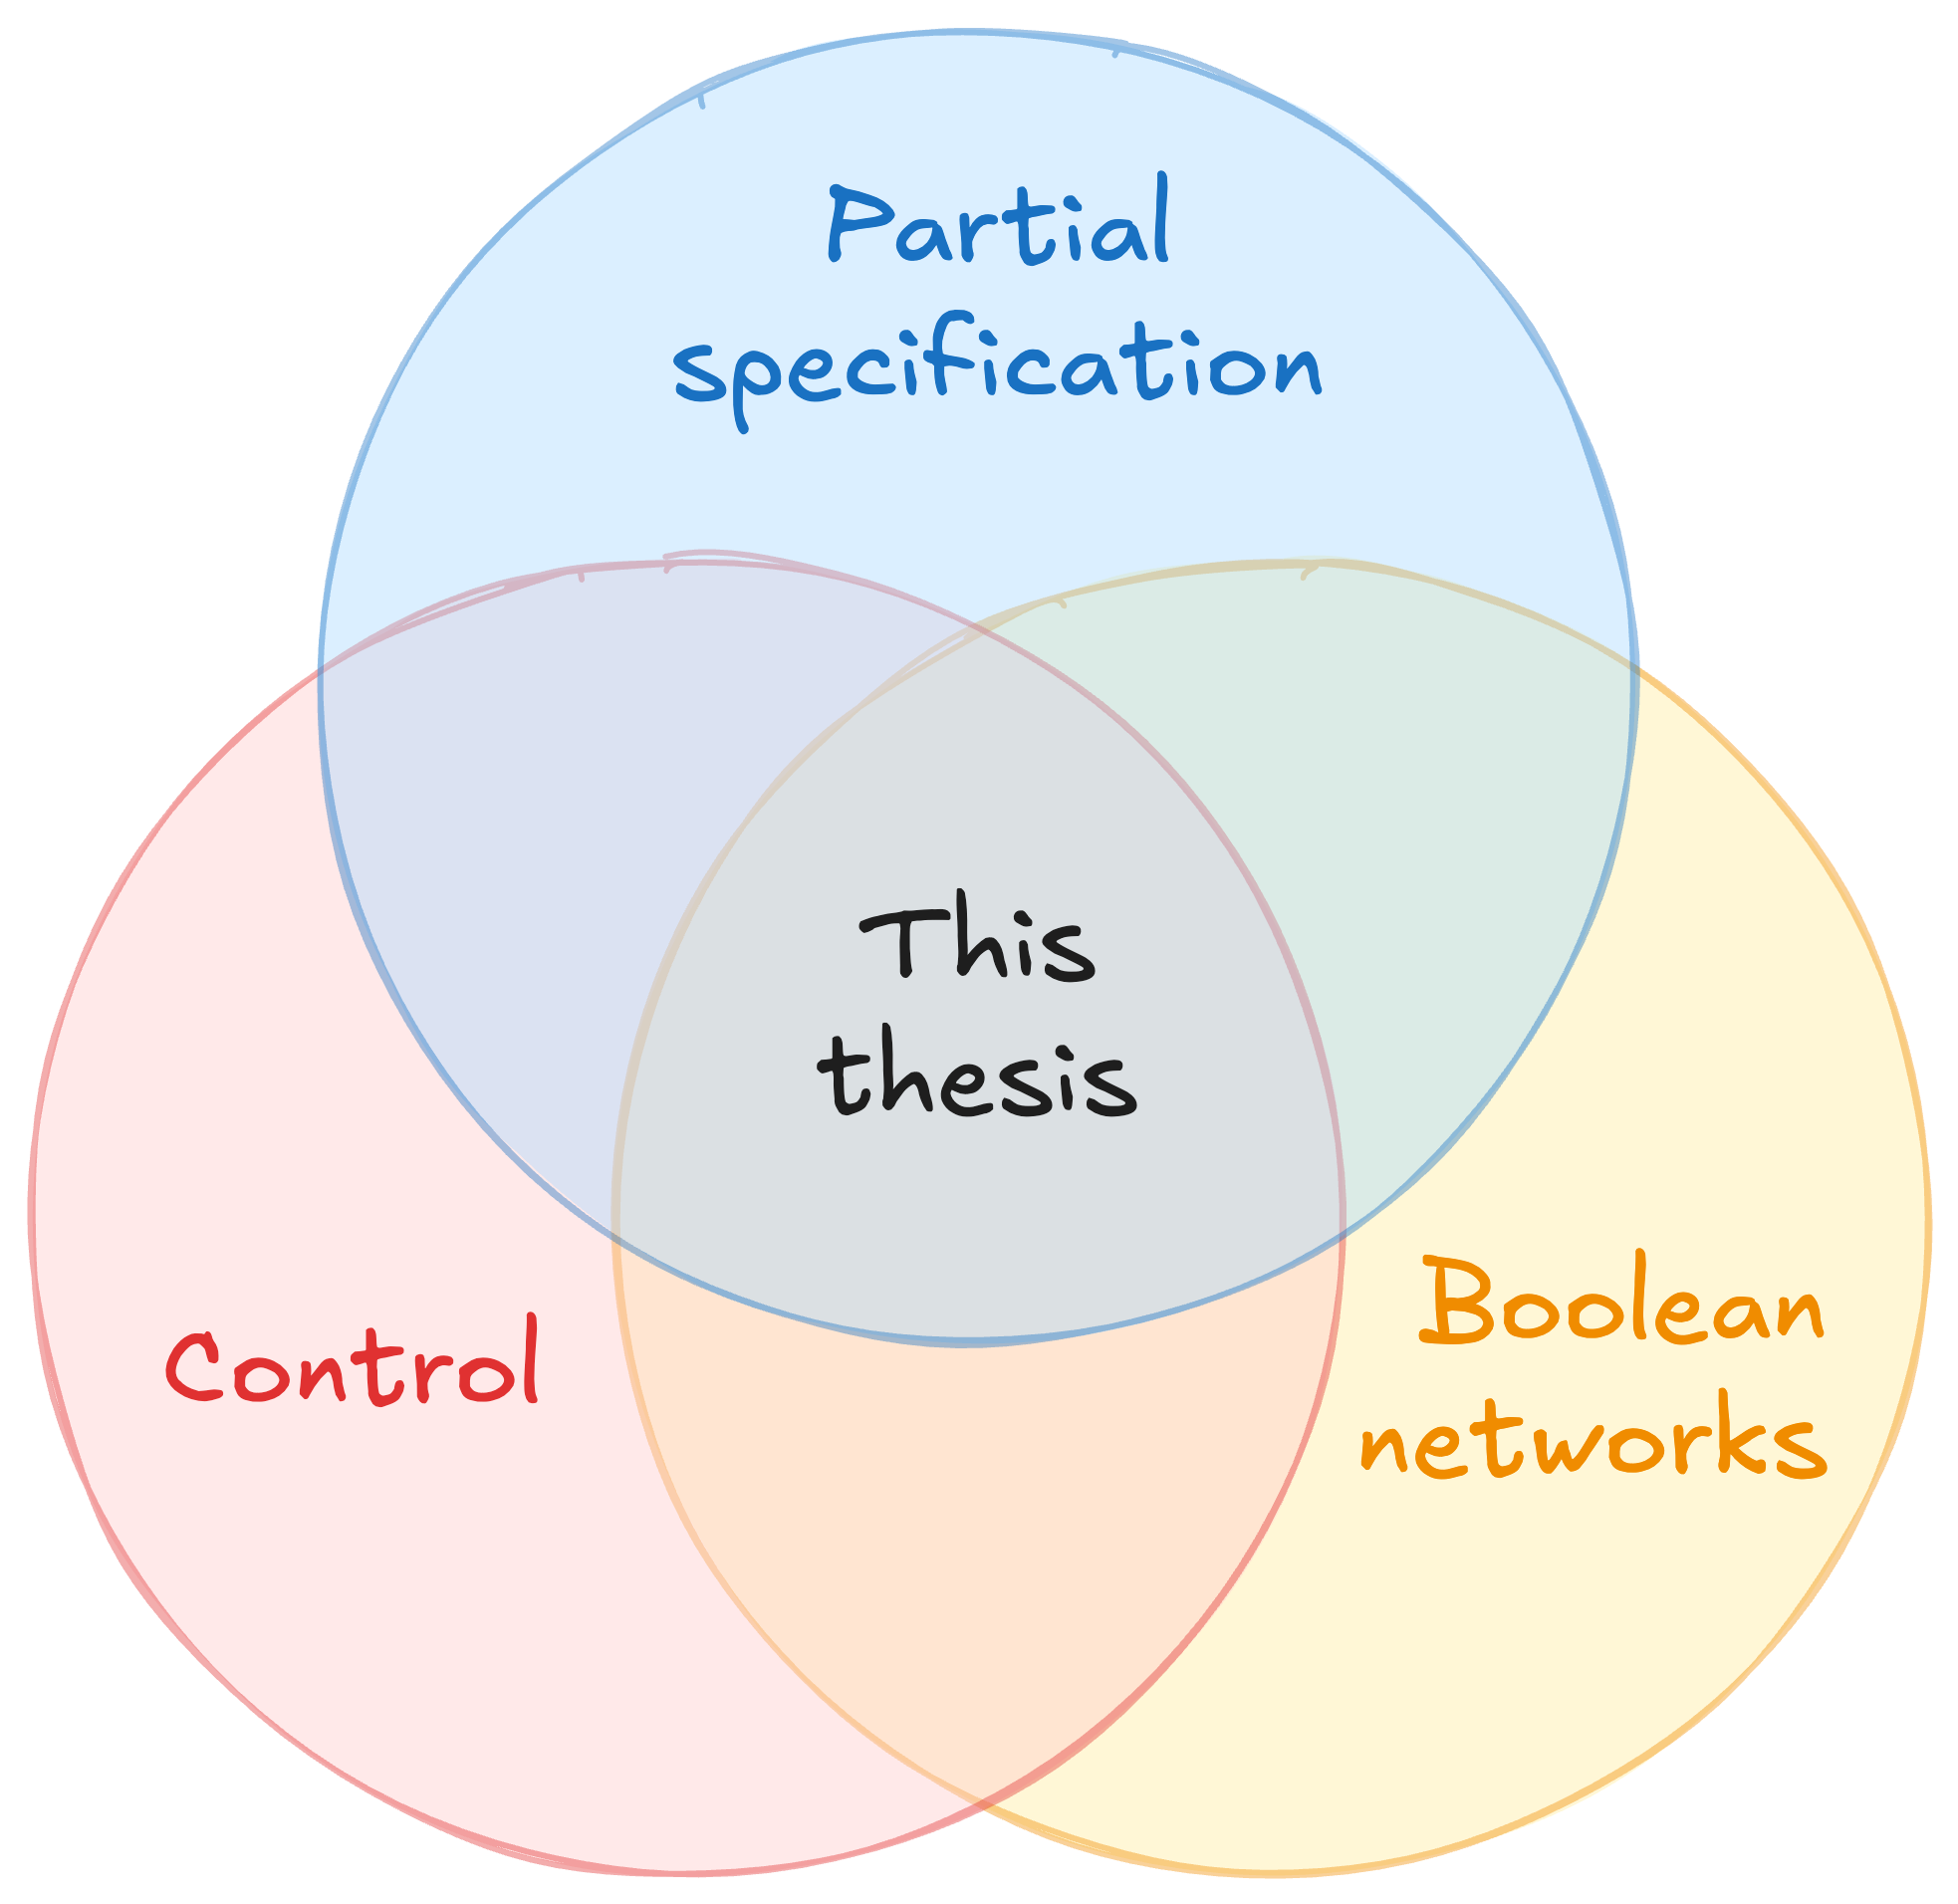
\includegraphics[width=0.5\textwidth]{Figures/topics.png}
    \caption{
        The confluence of concepts studied in this thesis. 
    }
    \label{fig:topics}
\end{figure}

The contribution of this thesis lies in its integration of three distinct concepts: control, asynchronous Boolean networks and systems with partial specification. Such a confluence has not yet been explored previously. The asynchronous Boolean networks are a well-studied model of system biology. Also, control is a commonly employed formal method in systems biology and the topic of controlling asynchronous BNs was already thoroughly studied as we describe in \autoref{s:control_of_bns}. On the contrary, the promising model of partially specified Boolean networks is just beginning its rise. Other formal methods such as attractor search~\cite{Benes2021, Roncalli2022}, bifurcation~\cite{Benes2022}, or parameter synthesis~\cite{Benes2023} are also being investigated only relatively recently.
 
The partial specification of BNs thus makes this work truly novel, although the specific approaches are often inspired by previously investigated intersections of the topics as we will see in the thesis. The objectives of this thesis are four-fold:

\begin{enumerate}
    \item Formally define control problem for partially specified Boolean networks
    \item Develop efficient methods that solve the control problem for partially specified Boolean networks 
    \item Bundle the developed methods to a software toolkit
    \item Demonstrate applicability for biological systems
\end{enumerate}

Now let us have a look at these goals in detail and describe in what parts of this thesis they are fulfilled.

\medskip

\noindent\PrimaryColor{\spacedlowsmallcaps{Goal 1 -- Problem definition.}}\hspace{3pt} Problem definition is an essential contribution of this work since the problem of \PBN{} control has not been formalized prior to my work. Several crucial aspects need to be considered for the problem definition. Firstly, attractors of the \PBN{} vary according to the interpretation. Therefore, searching for non-permanent perturbations that drive the network into a target attractor would be impossible for interpretations of unknown parts, where the given attractor is not present in the first place. Secondly, the practical realization of perturbations requires non-trivial effort; therefore, in a normal BN setting the number of perturbations is sought to be minimal. However, there is rarely a solution with a few perturbations in the partially specified setting, which would work for a big portion of interpretations. Thus, optimization criteria should be readjusted accordingly. 

The achievement of this goal is presented in \autoref{s:source_target_problem_definition} where we define \emph{source-target} control for \PBN{} which result is a relation of perturbations with interpretations for which they work as opposed to standard control goal where only minimal perturbation sets are returned. However, the landscape of attractors may change between interpretations~\cite{Benes2022}. That might cause a shift of target attractors that is not impeding from the cell reprogramming objective, but it is technically not allowed by a source-target control. This caveat is resolved by a more general notion of control -- \emph{phenotype} control which is defined in \autoref{s:phenotype_problem_definition} where only target traits are necessary to be known in advance.

\medskip


\noindent\PrimaryColor{\spacedlowsmallcaps{Goal 2 -- Efficient methods development.}}\hspace{3pt} As described before, the control problem for fully specified asynchronous BNs has been well-studied already. Therefore, after control for \PBN{} is formally defined, in theory, we could use the existing methods for asynchronous BN control to solve the problem for every interpretation distinctly. However, the number of these interpretations can be doubly exponential, meaning even a very efficient method for BN control would need to be run too many times to be handled in a realistic time. That is why seeking a novel, efficient approach for the partially specified setting is crucial.

Three methods were developed to solve the posed variants of the problem.

\begin{enumerate}
    \item Parallel one-step source-target control method for \PBN{} with semi-symbolic state space exploration and symbolic result which is described in \autoref{sec:target_semisymbolic}~\cite{Brim2021}
    \item One-step, temporary, and permanent source-target control for \PBN{} with symbolic state space exploration and symbolic result which are described in \autoref{sec:ostp_symbolic}~\cite{brim2022}
    \item Permanent phenotype control method with symbolic state space exploration for \PBN{} and result requiring explicit enumeration which is described in \autoref{chapter:phenotype_control_psbn}~\cite{Benes2023b}
\end{enumerate}

The aforementioned sections present algorithms, and simple (i.e., quantitative) demonstrations of them.

\medskip

\noindent\PrimaryColor{\spacedlowsmallcaps{Goal 3 -- Software toolkit for methods.}} \hspace{3pt} In order to make the developed methods publicly available, they were incorporated to the BioDivine toolkit~\cite{Barnat2009}. A library in Rust based on AEON tool~\cite{aeon} was developed to make methods fast and performant. Later, the library was wrapped into Python language as part of AEON.py tool~\cite{aeonpy}. This helps to make the methods more convenient to work with for the wider scientific audience because the language is easier to learn and offers popular notebook environments such as JuPyter~\cite{Barba2021}. The Python version also has become part of the CoLoMoTo Interactive Notebook tools~\cite{Naldi2015,Levy2018}. Finally, the control functionality was also embedded into AEON web application~\cite{Vesely2025}. The software technical specification and solved challenges are in detail described in \autoref{chapter:software}.

\medskip

\noindent\PrimaryColor{\spacedlowsmallcaps{Goal 4 -- Applications to biological systems.}}\hspace{3pt}
Finally, since Boolean network control is closely connected to cell reprogramming, we demonstrate that the developed methods address the original biological motivation of this thesis. In addition, we show that control can also serve as a tool for model refinement. Both applications, together with case studies illustrating their utility, are presented in \autoref{chapter:applications}.

\section{Thesis structure}

As mentioned before, this thesis covers multiple interlaced themes. Thus, it is important for the reader to recognize what aspects are considered while reading this thesis, especially distinguishing where only fully specified Boolean networks are discussed and where their partial specification is assumed. To help with that, a switch from the context be indicated by accompanying figure in the margin of the text, similar to one in \autoref{fig:topics}. Also, in the following text we provide a brief guidance on the structure of the thesis and what is covered in each chapter.

\autoref{chap:prelim} describes all necessary preliminaries to understand the basic problematic of the fully specified Boolean networks. Regulatory networks, which are an essential basis for BNs and also \PBN{s} are described at first (\autoref{s:reg_net}). Then, all motivation and formal definitions related to fully specified BNs are introduced (\autoref{section:boolean-networks}). After that, the control problem for BNs, is described, including technical differences between all variants of the problem (\autoref{s:control_of_bns}). Finally, the notion of partially specified Boolean networks is introduced (\autoref{s:psbn}), including the motivation for this model and the technical details of it.

\autoref{chap:sota} is about the state of the art in the field of control of Boolean networks. It covers the methods for control from the most general classes of the systems to the systems most similar to the \PBN{}s. First, it describes roots of the control theory in terms of discrete systems (\autoref{sec:controlDiscrete}) and incompletely specified systems (\autoref{sec:controlPartiallySpecified}). Then, it describes the methods for control of fully specified BNs from the simplest synchronous BNs (\autoref{sec:controlSynchronous}) to the more complex asynchronous (\autoref{sec:controlAsynchronous}) and most-permissive BNs (\autoref{sec:controlMostPermissive}). Finally, it describes how the control problem for BNs can aid the problem of model refinement (\autoref{sec:controlInference}) and a comparison of the software tools for control of BNs is given (\autoref{sec:relatedTools}).

\autoref{chapter:source_target_control} provides the problem definition of source-target control problem for \PBN{} (\autoref{s:source_target_problem_definition}) and then it also shows two methods that solve this problem. The first one, semi-symbolic and parallel uses only the most trivial one-step perturbation (\autoref{sec:target_semisymbolic}). The later developed fully symbolic method is capable of one-step, temporary and permanent perturbations (\autoref{sec:ostp_symbolic}). Finally, these two methods are discussed and compared (\autoref{sec:control_evaluation}).

\autoref{chapter:phenotype_control_psbn} describes the problem of phenotype control for \PBN{} (\autoref{s:phenotype_problem_definition}) and a method to solve it (\autoref{sec:phen_control_method}). The method is based on the same symbolic state space exploration as the one for source-target control. Finally, the method is evaluated on several middle-sized \PBN{}s (\autoref{sec:phen_control_evaluation}) in terms of performance and the quality of the results. 

\autoref{chapter:software} describes the software implementation of the presented methods. First, the software architecture is described (\autoref{sec:software_architecture}), including the main libraries and their functionalities (\autoref{sec:core_packages}). Then, the web application for control of \PBN{} is presented (\autoref{sec:aeon_web_app}), followed by the description of the Python package (\autoref{sec:python_package}).

\autoref{chapter:applications} is about the applications of the developed methods for control of \PBN{}. Firstly, it described the primary motivation for this work -- the problem of cell reprogramming in regenerative medicine (\autoref{sec:cell_reprogramming}). Then, it shows an example of \PBN{} control application for cell reprogramming on a specific example of a myeloid cell (\autoref{sec:myeloid_case_study}). After that, a more general workflow of how the control of \PBN{} can be used to design a therapy or to refine the model is described (\autoref{sec:control_workflow}). Finally, this workflow is shown on the second case study that is focused on the MAPK signalling pathway and demonstrates the control-guided model refinement (\autoref{sec:mapk_case_study}).

Finally, \autoref{chapter:conclusion} summarizes the main contributions of this thesis and discusses possible future directions for research in this area.

\chapter{Preliminaries}
\label{chap:prelim}

This chapter provides the necessary background to understand the concepts and models used throughout the thesis. First, we introduce the concept of regulatory networks as abstract representations of interactions between biological components (\autoref{s:reg_net}). Building on this foundation, we formally define Boolean networks in \autoref{section:boolean-networks}, which serve as the core modeling framework throughout this thesis. With this model in place, we turn to the control of Boolean networks and explore various control strategies in \autoref{s:control_of_bns}. Finally, we extend the classical framework to partially specified Boolean networks in \autoref{s:psbn}, a novel model variant that incorporates uncertainty and incomplete knowledge.

\section{Regulatory networks}
\label{s:reg_net}

% RNs are the basis for BNs, they are designed first
The model designers of biological systems typically begin their work by identifying connections and influences among proteins, genes, and other biochemical substances. Such an approach is often chosen because gaining evidence for these kinds of interconnections is usually the most accessible. We may observe that in the presence or a lack of some substance, another is behaving differently. On the other hand, translating such interaction into an explicit mathematical form is more complex. 

The model that captures just simple relationships between biochemical substances (or other entities) is called regulatory networks (RNs)~\cite{davidson2005}. Consider an example in \autoref{fig:regulatory_network}. It compactly represents a relationship between three enzymes and proteins. For example, we can observe transitive feedback between network components. Influencing FGFR3 could impact the whole rest of the network, while by contrast, perturbing ERK would not affect FGFR3 at all.

\begin{figure}[htp]
    \begin{centering}
    \centering
    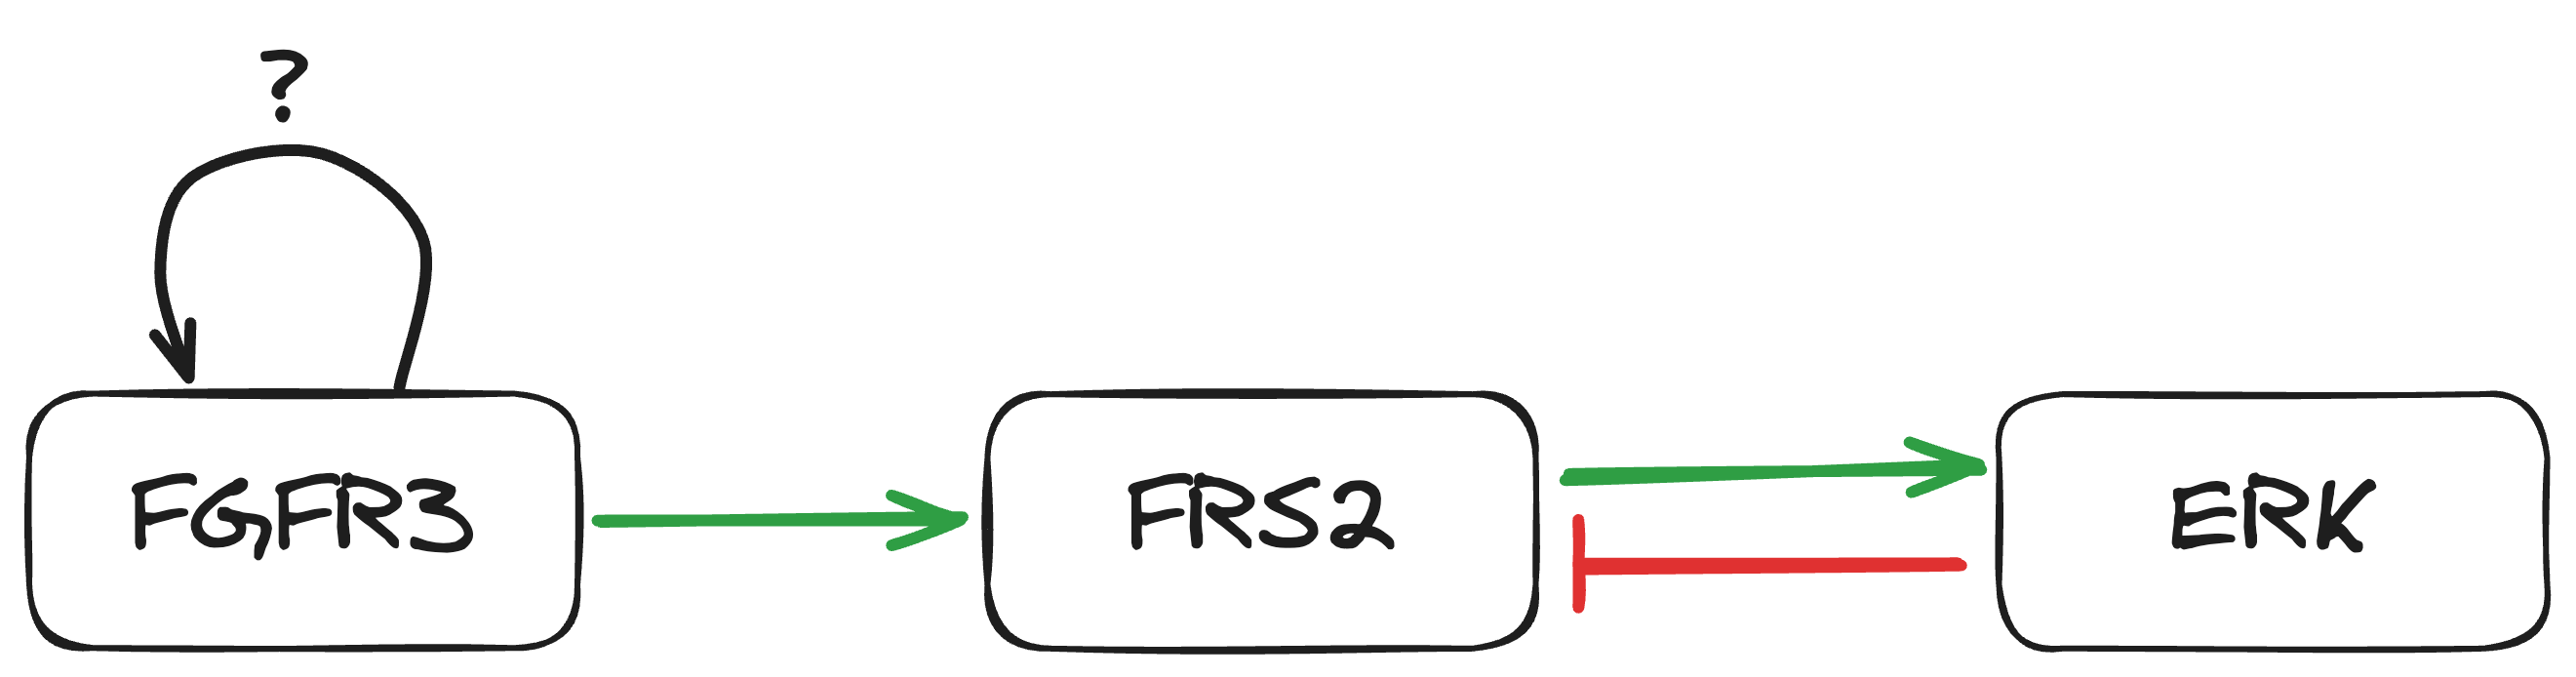
\includegraphics[width=0.6\textwidth]{Figures/regulatory_network.png}
    \caption{\textbf{An example of a simple regulatory network.} The RN contains three nodes and four regulations (two activations, one inhibition and one non-essential self-regulation). The network is a small extract of a MAPK signaling pathway from~\cite{Grieco2013}.} 
    \label{fig:regulatory_network}
    \end{centering}
\end{figure}

\begin{definition}
    Let $\rnMath = (\vertices, \edges)$ denote a directed graph representing the regulatory network, where $\vertices$ is the set of vertices representing the molecular components and $\edges \subseteq \vertices \times \vertices$ is the set of directed edges representing the regulatory interactions between the components.
\end{definition}

% Activations, inhibitions
We call the influence of one substance (regulator) to another (target) a \emph{regulation}. These regulatory effects typically fall into two categories: upregulation (activation), which denotes a positive influence (usually represented in green), or downregulation (inhibition), indicating a negative effect (depicted in red). These types of regulations are \emph{monotonous}; since their impact is consistent. Non-monotonous regulations appear in biological models rarely. When they occur or if the monotonicity is not required, they are depicted in a black color. 

% Observability 
Apart from the monotonicity, another aspect we consider of regulation is \emph{observability}. Observable (essential) regulations were proven by experimentation that the regulator surely influences the target. I.e., in some settings where the regulator is present the regulated substance behaves differently compared to the environment with the lack of the regulator. On the contrary, in case we do not have this certainty, the regulation is \emph{non-essential}. The non-essential regulations should not be over-used. Hypothetically, we could mark all possible RN edges with this type of regulation resulting in a complete, dense graph giving us very little information. Nonetheless, if these regulations occur, they are labelled by a question mark. All other regulations are considered to be observable. We give more formal details about different regulation types in \autoref{ss:bn_definition}.


% RNs are too abstract to be that helpful, we need BN.
Notice, that the influences captured by RNs are highly abstract and that there is very little modeling knowledge present in this model. That is why more specific models are using RNs as a basis. Among these models are ODEs, stochastic gene networks, or Boolean networks, which are described next.


\section{Boolean networks}
\marginpar{
    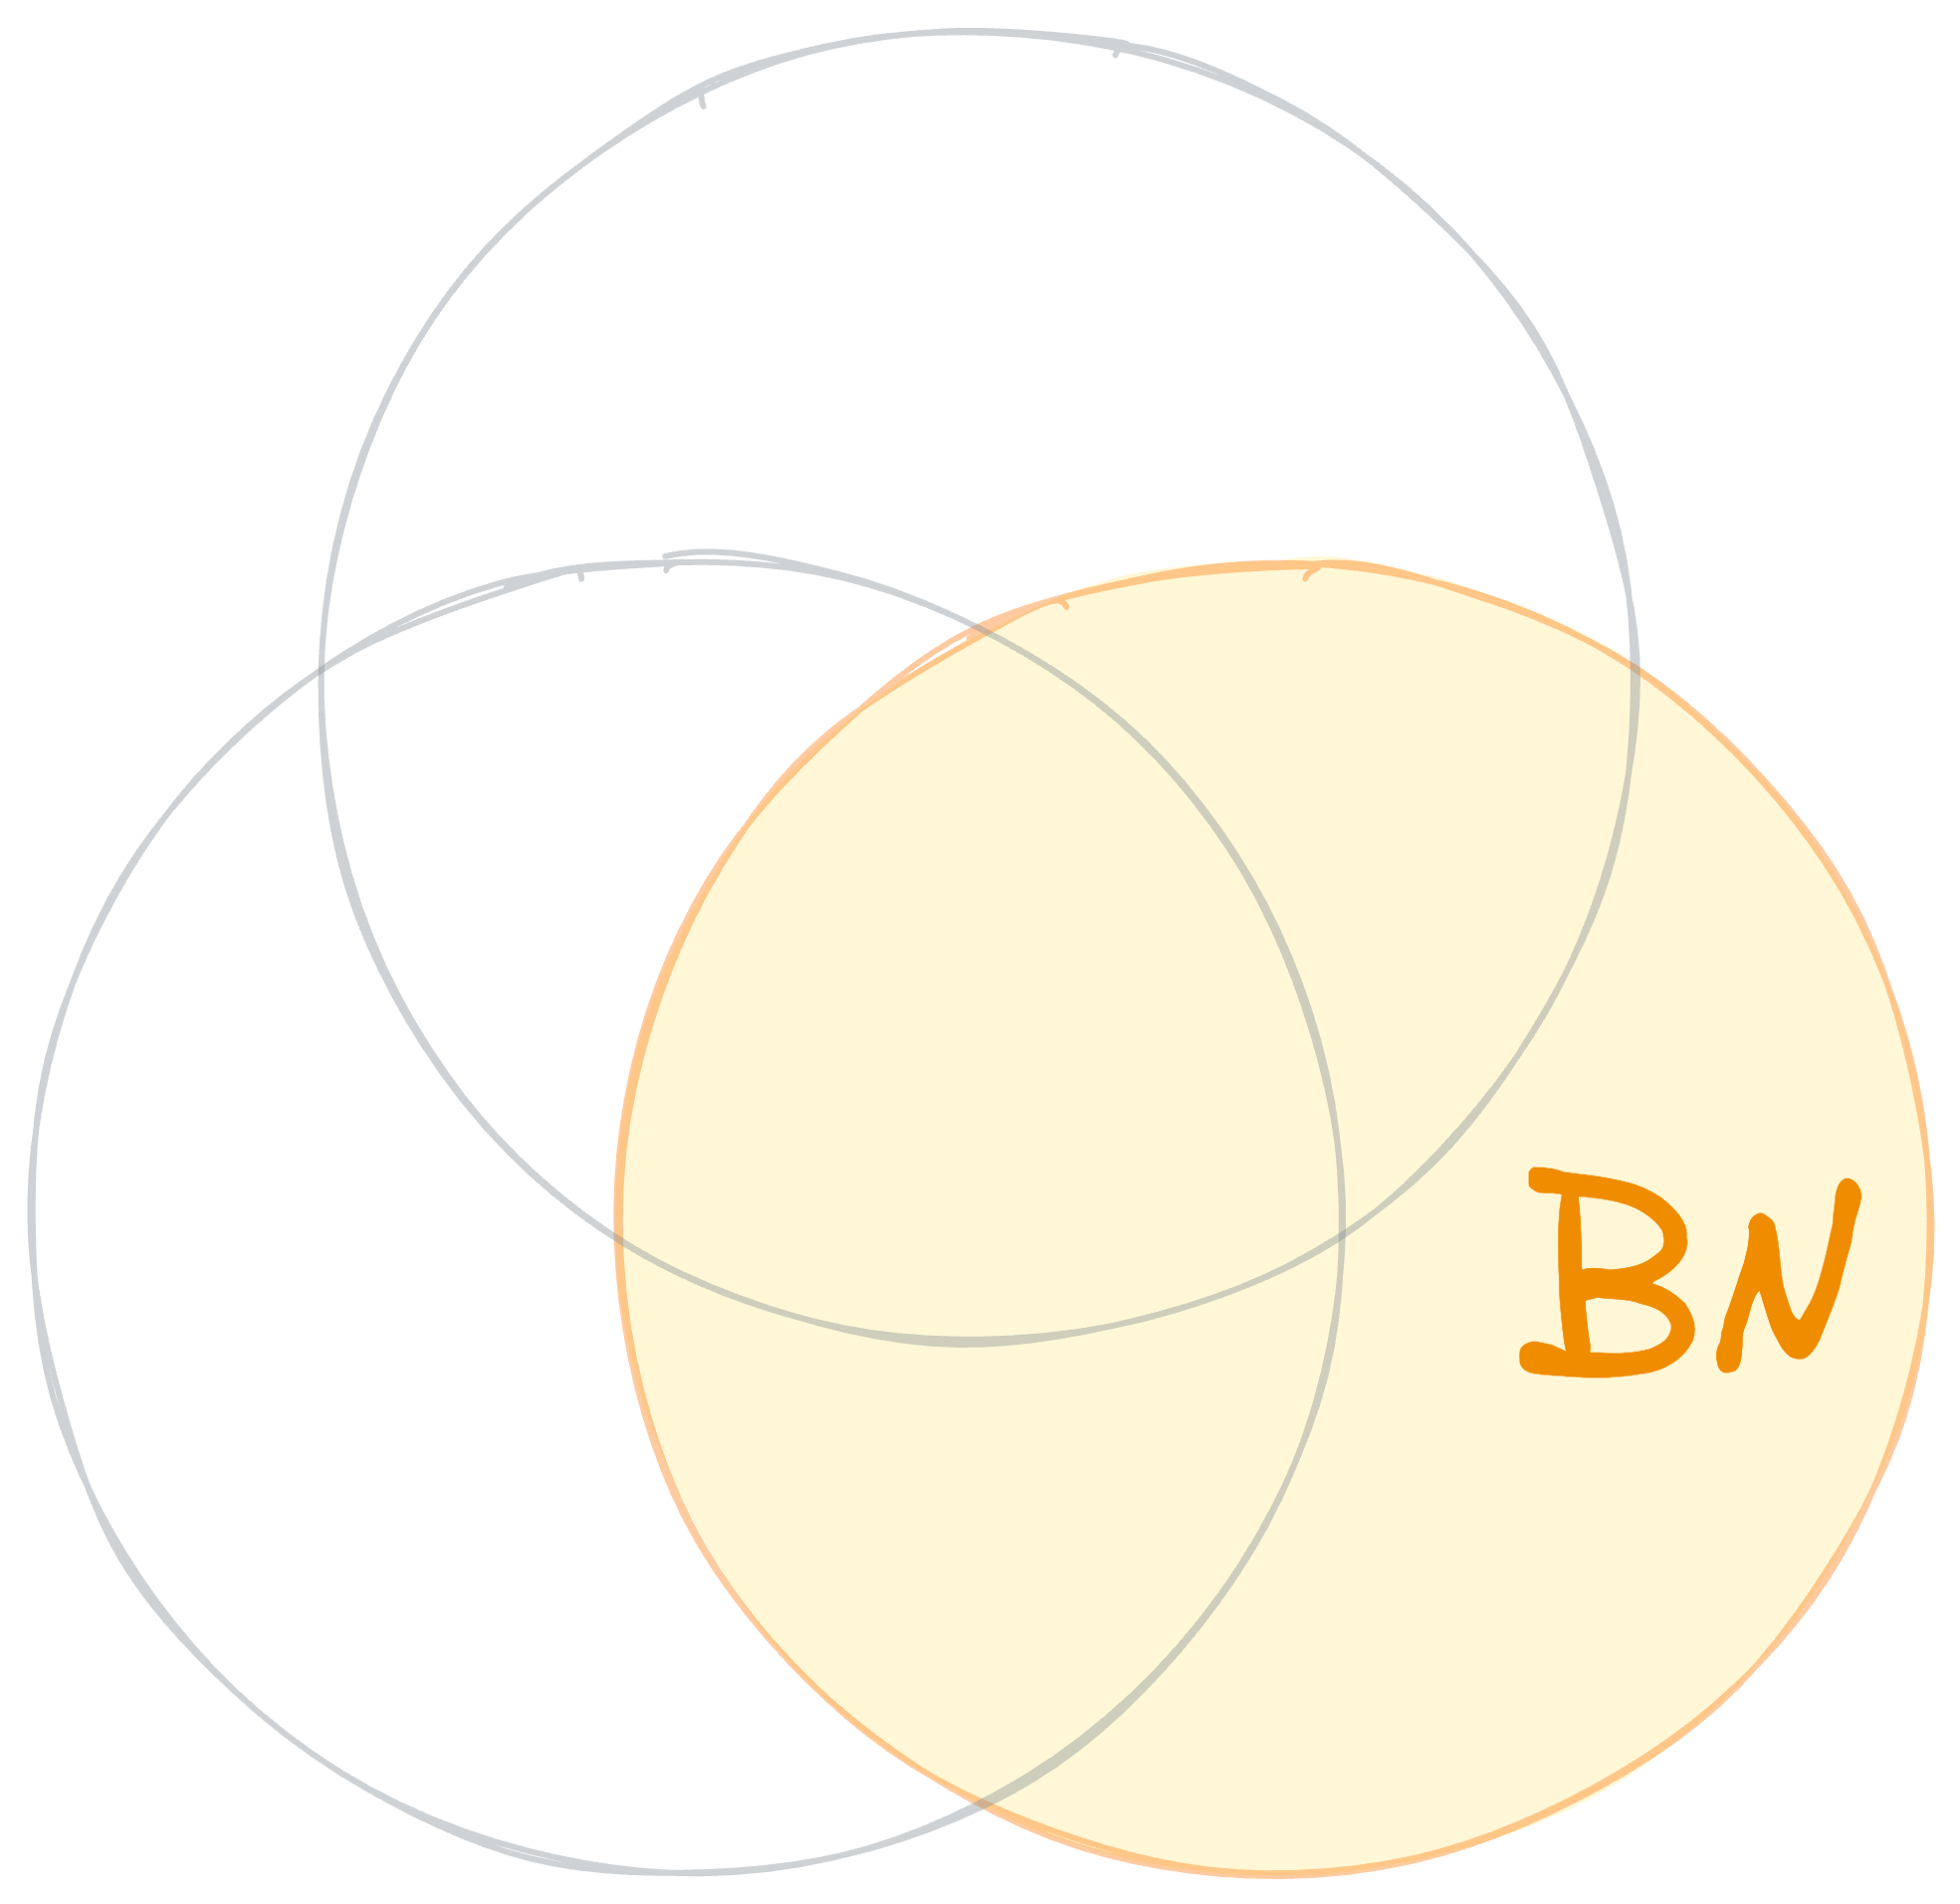
\includegraphics[width=\marginparwidth]{Figures/topics_bns.png}
}
\label{section:boolean-networks}

% Many interactions in biology -> BNs solve this 
The traditional differential equation-based (ODE) models often struggle to capture the intricate interactions and feedback loops present in biological systems due to their complexity. This shortcoming was addressed by Boolean networks (BNs) that were introduced by Kauffman in the 1960s~\cite{Kauffman1969}. Kauffman represented system components as binary variables connected by logical rules. Such an abstraction facilitated the exploration of system dynamics while avoiding the computational complexity of traditional models. 

Since then, it has become a widely used model to study the dynamics of complex biological systems~\cite{Barbuti2020,albert2004}. The Boolean representation also allows researchers to focus on the regulatory relationships and dynamics without getting hindered by detailed biochemical mechanisms. This simplification facilitates efficient analysis of regulatory networks, enabling the discovery of crucial pathways, prediction of system behavior, and identification of pivotal components driving cellular processes.
% Biological systems are characterized by a high amount of interacting elements and their interactions. The Boolean networks (BNs) offer a valuable approach for modeling regulatory networks, providing a way to maintain the structural complexity while ensuring computational feasibility. 

\subsection{Notation}

Here, the notation used in the context of Boolean networks is briefly summarized. For a complete overview of the used notation, refer to \autoref{app:notation}

We consider $0$ and $1$ as interchangeable with $\mathit{false}$ and $\mathit{true}$, respectively. We then define $\bools = \{ 0, 1 \}$ to be the set of Boolean values and $\bools_\unspecified = \{ 0, 1, {\unspecified} \}$ to be an extension of $\bools$ which also admits a \emph{free} value~$\unspecified$ (i.e.~neither $\mathit{true}$ nor $\mathit{false}$). We write $\bools^n$ to denote the set of all $n$-element vectors over $\bools$. For each $x \in \bools^n$, $x_i$ then denotes the $i$-th element of $x$. Finally, for $x \in \bools^n$, index $i \in [1,n]$, and a Boolean value $b \in \bools$, expression $x[i \mapsto b]$ denotes a substitution of the $i$-th element in $x$ for the value~$b$.  Formally, the result is $x' = x[i \mapsto b]$ s.t. $x'_j = b$ for $j = i$, and $x'_j = x_j$ otherwise.

\subsection{Definition}
\label{ss:bn_definition}

We can formally define Boolean networks, as follows:

\begin{definition}
	Let $n$ be the number of system variables. A \emph{Boolean network} is a collection $\bnMath = \{ f_1, \ldots, f_n \}$ with each $f_i: \bools^n \to \bools$ being the Boolean \emph{update function} (sometimes called \emph{local function}) of the network's $i$-th variable.
\end{definition}

A running example of a Boolean network based on the RN from \autoref{fig:regulatory_network} can be seen in \autoref{fig:bn_basic}. Note that, while it is mathematically more convenient to denote variables by their indices, oftentimes we will use their actual names (e.g. $\var{FGFR}$ instead of $f_1$) to present context of the biological system comprehensively.

\begin{figure}[htb]
    \centering
    \subfloat[Regulatory network]{
        \label{subfig:regulatory_network}
        \begin{minipage}[t]{0.35\textwidth}
        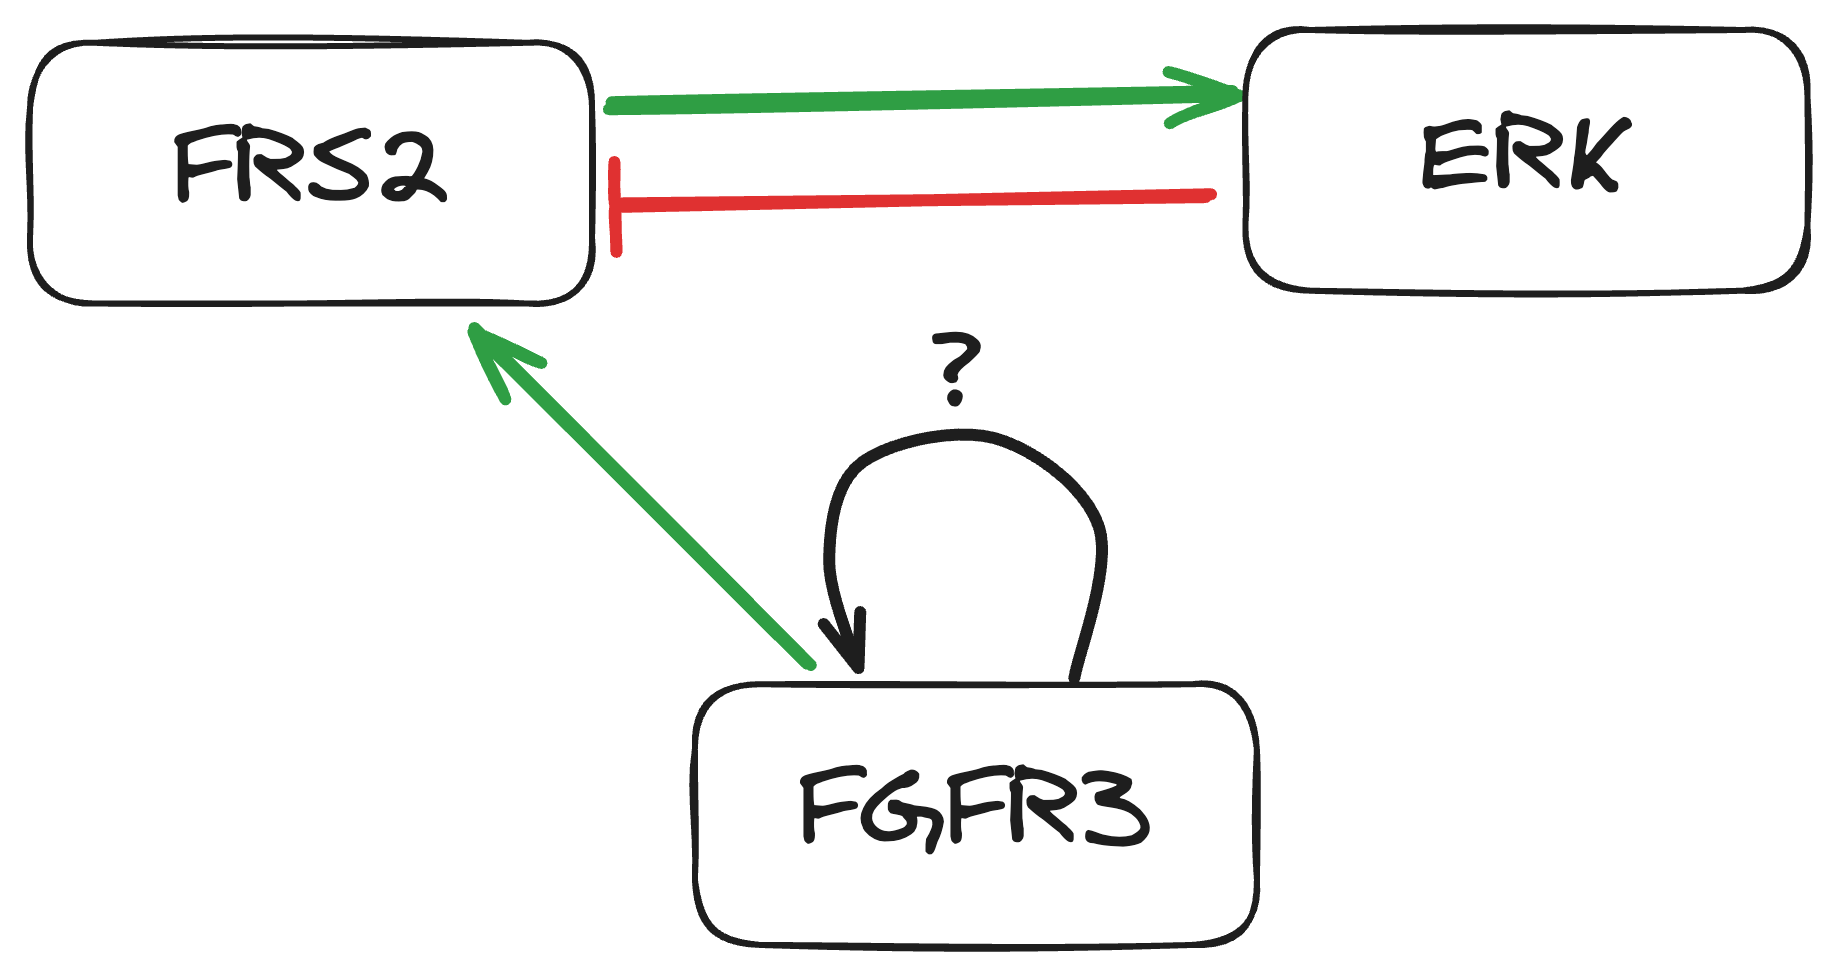
\includegraphics[width=\textwidth,valign=b]{Figures/regulatory_network2.png}
        \end{minipage}
    }
    \subfloat[Boolean network]{
        \label{subfig:bn}
        \begin{minipage}[b]{0.35\textwidth}
        \begin{align*}
            \var{FGFR} &= 1 \\
            \var{FRS2} &= \var{FGFR} \land \neg \var{ERK} \\
            \var{ERK} &= \var{FRS2}
        \end{align*}
        \end{minipage}
    }
    \newline
    \subfloat[State transition graph]{
        \label{subfig:stg}
        \begin{minipage}[t]{0.45\textwidth}
            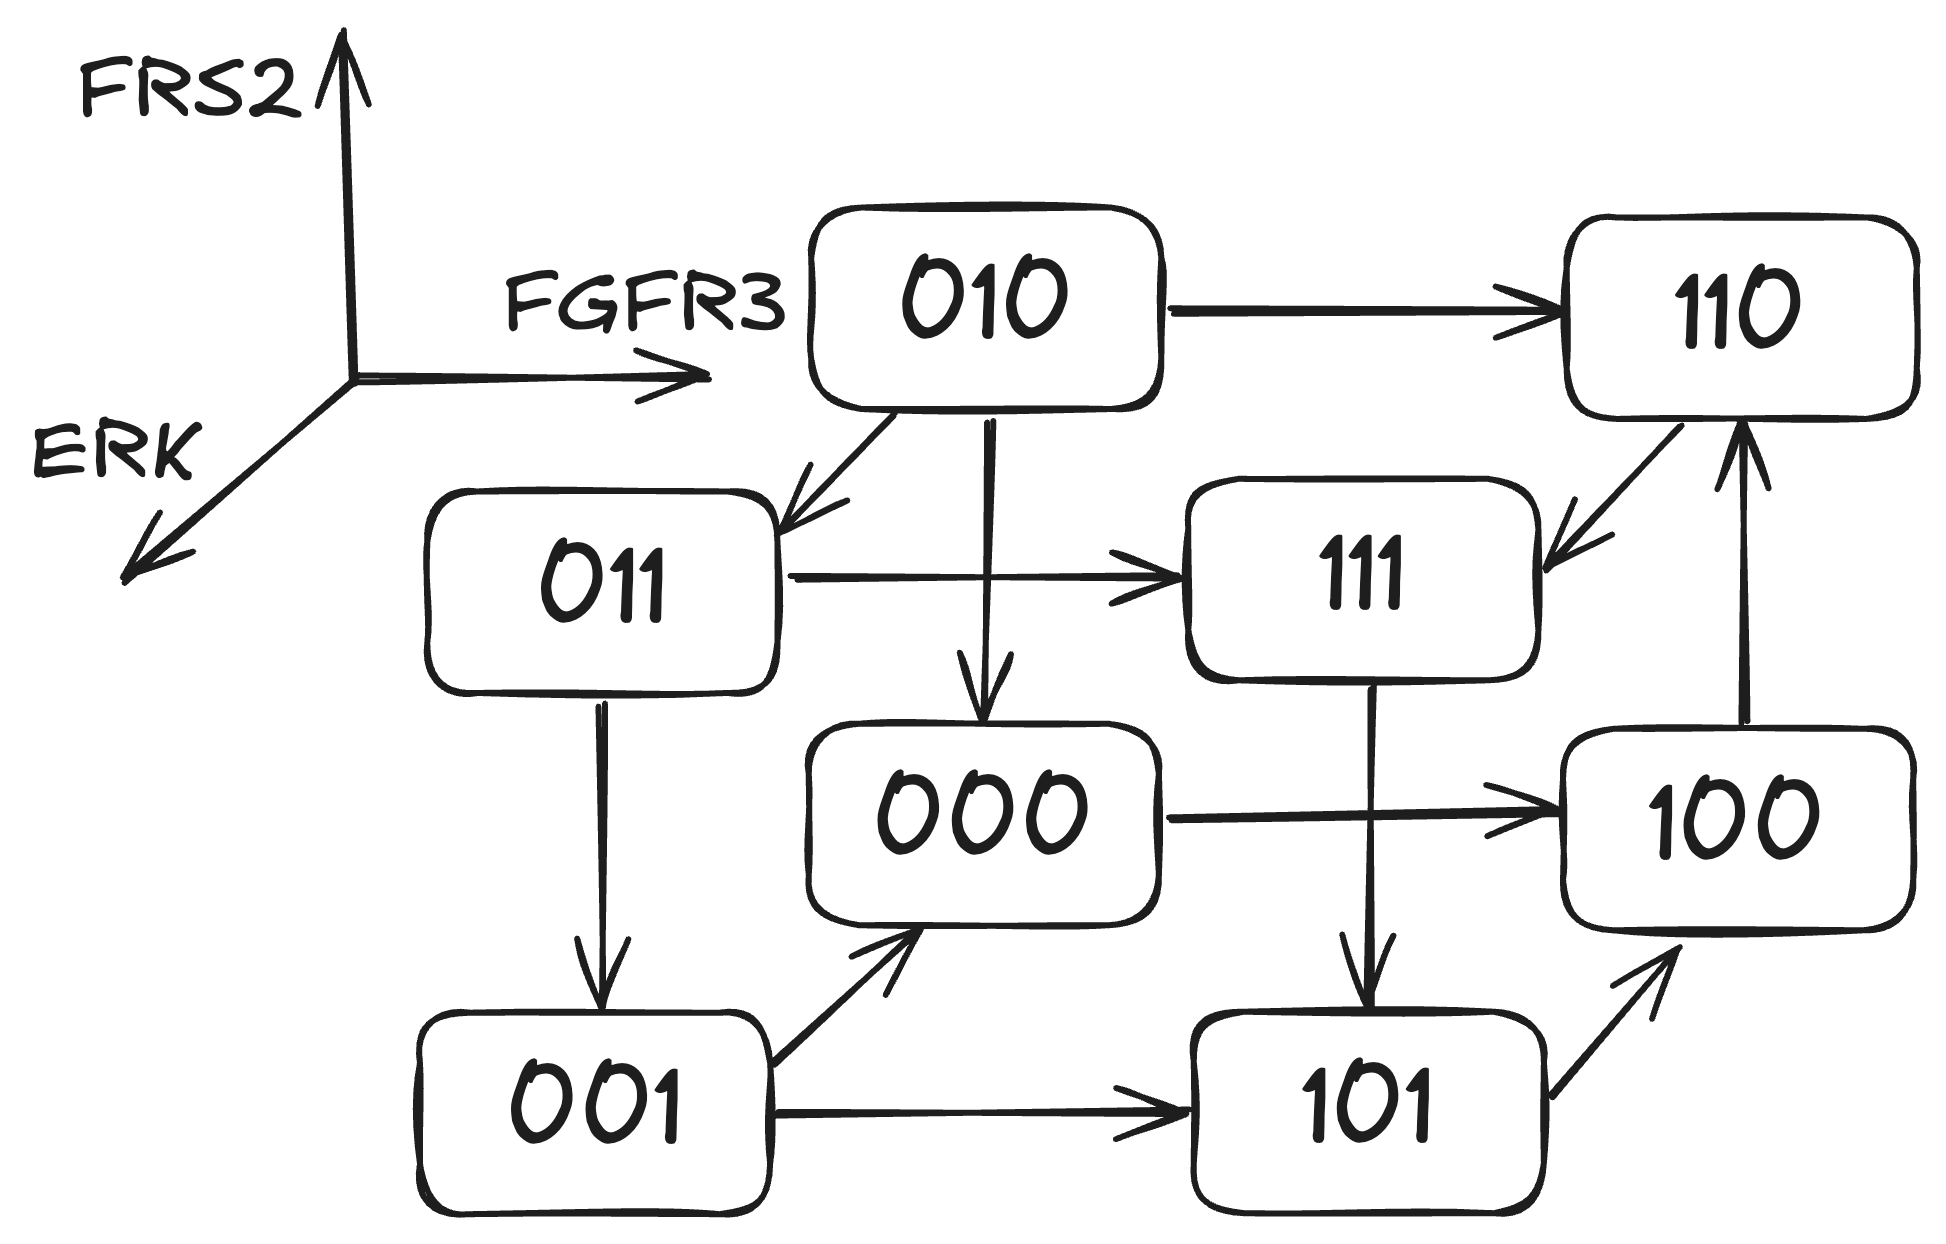
\includegraphics[width=\textwidth,valign=b]{Figures/state_space.png}
        \end{minipage}
    }
    \caption{\textbf{An example of a Boolean network and related concepts.} In \autoref{subfig:regulatory_network}, the same RN as in \autoref{fig:regulatory_network} is displayed for a reader's convenience. This RN is used as a basis for BN defined in \autoref{subfig:bn}. Finally, state-transition graph of the BN is shown in \autoref{subfig:stg} where the labeling of states has the same order as variables order in \autoref{subfig:bn}.} 
    \label{fig:bn_basic}
\end{figure}


% \intention{State space, a state, regulators, inputs, outputs} 
In the context of a specific Boolean network, the set $\bools^n$ is the network's \emph{state space}, and the vectors $x \in \bools^n$ are its \emph{states}. Note that although the input of each $f_i$ is a full state $x \in \bools^n$, the output of $f_i$ does not typically depend on all network variables, but rather on a smaller subset of variables which we say \emph{regulate} the $i$-th variable. These regulations are typically given by a corresponding regulation network. For a BN to respect the regulations defined by its regulation network, the function should comply with the regulation type in following ways:

\begin{itemize}
    \item If a variable $j$ is \emph{essential} for a variable $i$, denoted as $\essential(j,i)$ then: \\ $\exists x \in \bools^n . f_i(x[j \mapsto 1]) \neq f_i(x[j \mapsto 0])$
    \item If variable $j$ \emph{upregulates} (activates) variable $i$, denoted as $\activates(j,i)$: \\
    $ \forall x \in \bools^n . f_i(x[j \mapsto 0]) \Rightarrow f_i(x[j \mapsto 1])$
    \item If variable $j$ \emph{downregulates} (inhibits) variable $i$, or $\inhibits(j,i)$: \\ $\forall x \in \bools^n . f_i(x[j \mapsto 1]) \Rightarrow f_i(x[j \mapsto 0])$
\end{itemize}


If a variable has no regulators (i.e. its update function is a constant), we also call it an \emph{input} of $\bnMath$. Symmetrically, a variable that does not regulate any other variable is called an \emph{output}. For example, when we consider \autoref{subfig:regulatory_network}, if the self-regulation of FGFR3 was not present, FGFR3 would be considered an input.

% Subspaces
Additionally, we call the members of $\bools_\unspecified^n$ the \emph{subspaces} of $\mathbb{BN}$. Intuitively, each subspace $S \in \bools_\unspecified^n$ describes a hypercube in the state space $\bools^n$. This hyper-cube consists of states $x \in \bools^n$ such that $x_i = S_i$ for all $i$ where $S_i \in \bools$. We can thus treat each subspace $S$ as a set of states. Furthermore, to denote a specific subspace, we will often simply use a string of values from $\bools_\unspecified$ instead of the full vector notation (e.g. $S = 11\unspecified0$ instead of $S = (1,1,\unspecified,0)$).	

\subsection{Updating schema}
\label{ss:updating_schemes}

%Briefly discuss synchronous, async and most permisive
In our work, we focus on \emph{asynchronous} semantics for Boolean networks. To give a reader a better overview of the differences between the various semantics, we briefly discuss other common semantics and their trade-offs. A more formal and detailed guide to BN semantics can be found in~\cite{Pauleve2023b}.

In Boolean network modeling, the semantics used to define the update rules of node states significantly influence the system's dynamics and interpretability. \emph{Synchronous} semantics, as introduced in~\cite{Kauffman1969}, operate under the assumption that all nodes in the network update their states simultaneously in discrete time steps. While this approach simplifies analysis and yields deterministic behavior, it imposes an unrealistic constraint on systems such as gene regulatory networks, where simultaneous updating is biologically implausible.

In contrast, \emph{asynchronous} semantics, introduced in~\cite{Thomas1973}, allow for only one node to update at each time step, with a nondeterministic choice of which node updates. This reflects the inherent variability in timing and activity across components in real-world systems, such as the stochastic firing of genes. Asynchronous semantics maintain a more biologically and physically faithful representation of dynamics without the need to introduce explicit timing or probability.

\emph{Probabilistic} semantics introduce randomness directly into the update process. A variable has assigned more than a single update function, while each update function has assigned probability of triggering. This allows the modeling of noise and uncertainty but requires a probabilistic framework and often obscures causal interpretability. 

Lastly, the \emph{most permissive} semantics that was recently introduced in~\cite{Pauleve2020}, define all logically consistent transitions as simultaneously valid, capturing the broadest possible behavior. This is achieved by considering a transient state between 0 and 1 for each variable, allowing any combination of variables to update in a way that is consistent with their logical functions. While useful for exhaustive exploration, this framework might be hard to use for quantification of state-space components since these properties are lost to the abstraction via transient states.

Asynchronous semantics offer a compelling middle ground. They provide a natural and realistic modeling framework for systems where the order and timing of updates are nondeterministic. Nonetheless, they preserve the causal structure of networks and allow for quantifiable tractable analysis while avoiding the oversimplification of synchronous updates.

% STG
To formally reason about the evolution of the network's state, we consider asynchronous state-transition graph of BNs:

\begin{definition}
	Given a Boolean network $\mathbb{\bnMath} = \{ f_1, \ldots, f_n \}$, the \emph{state-transition graph} $\STG(\bnMath) = (\vertices, \edges)$ is a directed graph with $\vertices = \bools^n$ and $\edges \subseteq \vertices \times \vertices$ given as follows:
	$$
		(u,v) \in \edges \Leftrightarrow (u \not= v \land \exists i \in [1,n].~v = u[i \mapsto f_i(u)])
	$$
\end{definition}

The \emph{state-transition graph} $\STG(\bnMath)$ captures the dynamics of the Boolean network by representing its states and transitions. An example is graphically depicted in \autoref{subfig:stg}.

% \intention{Maximal fair runs} 
The behavior of a network is then studied through its \emph{maximal strongly fair runs}. Here, a maximal run $\run: \NatsZero \to \bools^n$ represents an infinite sequence of states where for every $t \in \NatsZero$, we have either $\run(t) = \run(t+1)$, or $\run(t) \to \run(t+1)$. That is, the state either remains constant, or updates according to $\STG(\bnMath)$. 

Furthermore, we are only concerned with \emph{strongly fair} runs~\cite{Abadi1995,Mandon2019CMSB}. These are runs which do not delay any available transition indefinitely. Formally, let $\run$ be a run and $x \in \bools^n$ a state that appears infinitely often in $\run$, such that $x \to y$ for some $y \in \bools^n$. Then $\run$ is fair only if $y$ also appears infinitely often in $\run$ as a successor to $x$. To denote the set of such states that appear infinitely often in a run $\run$, we write $inf(\run) = \{ x \in \bools^n \mid \forall k \in \NatsZero, \exists t > k.~\run(t) = x \}$. Finally, we may write $x \in \run$ as a shorthand for $\exists t.~\run(t) = x$ and a set of all possible runs in $\bnMath$ is denoted as $\allRuns(\bnMath)$.

\subsection{State space structures}
\label{ss:state_space_structures}

% \intention{Bridge to state space structures} 
The focus on strongly fair runs naturally leads to the notions of trap set, trap space, and attractor, which dictate the long-term behavior of the corresponding BN:

\begin{definition}
	Let $\bnMath = \{ f_1, \ldots, f_n \}$ be a Boolean network and $X \subseteq \bools^n$ a set of network states. We say that $X$ is a \emph{trap set} when for all $x \in X$ and $y \in \bools^n$ we have that $x \to y$ implies $y \in X$ (i.e., $X$ cannot be escaped). A subspace $X = \bools^n_\unspecified$ which is also a trap set can be also called a \emph{trap space}. The $X$ is an \emph{attractor} when $X$ is strongly connected within $\STG(\bnMath)$.
\end{definition}

\begin{figure}[bth]
    \centering
    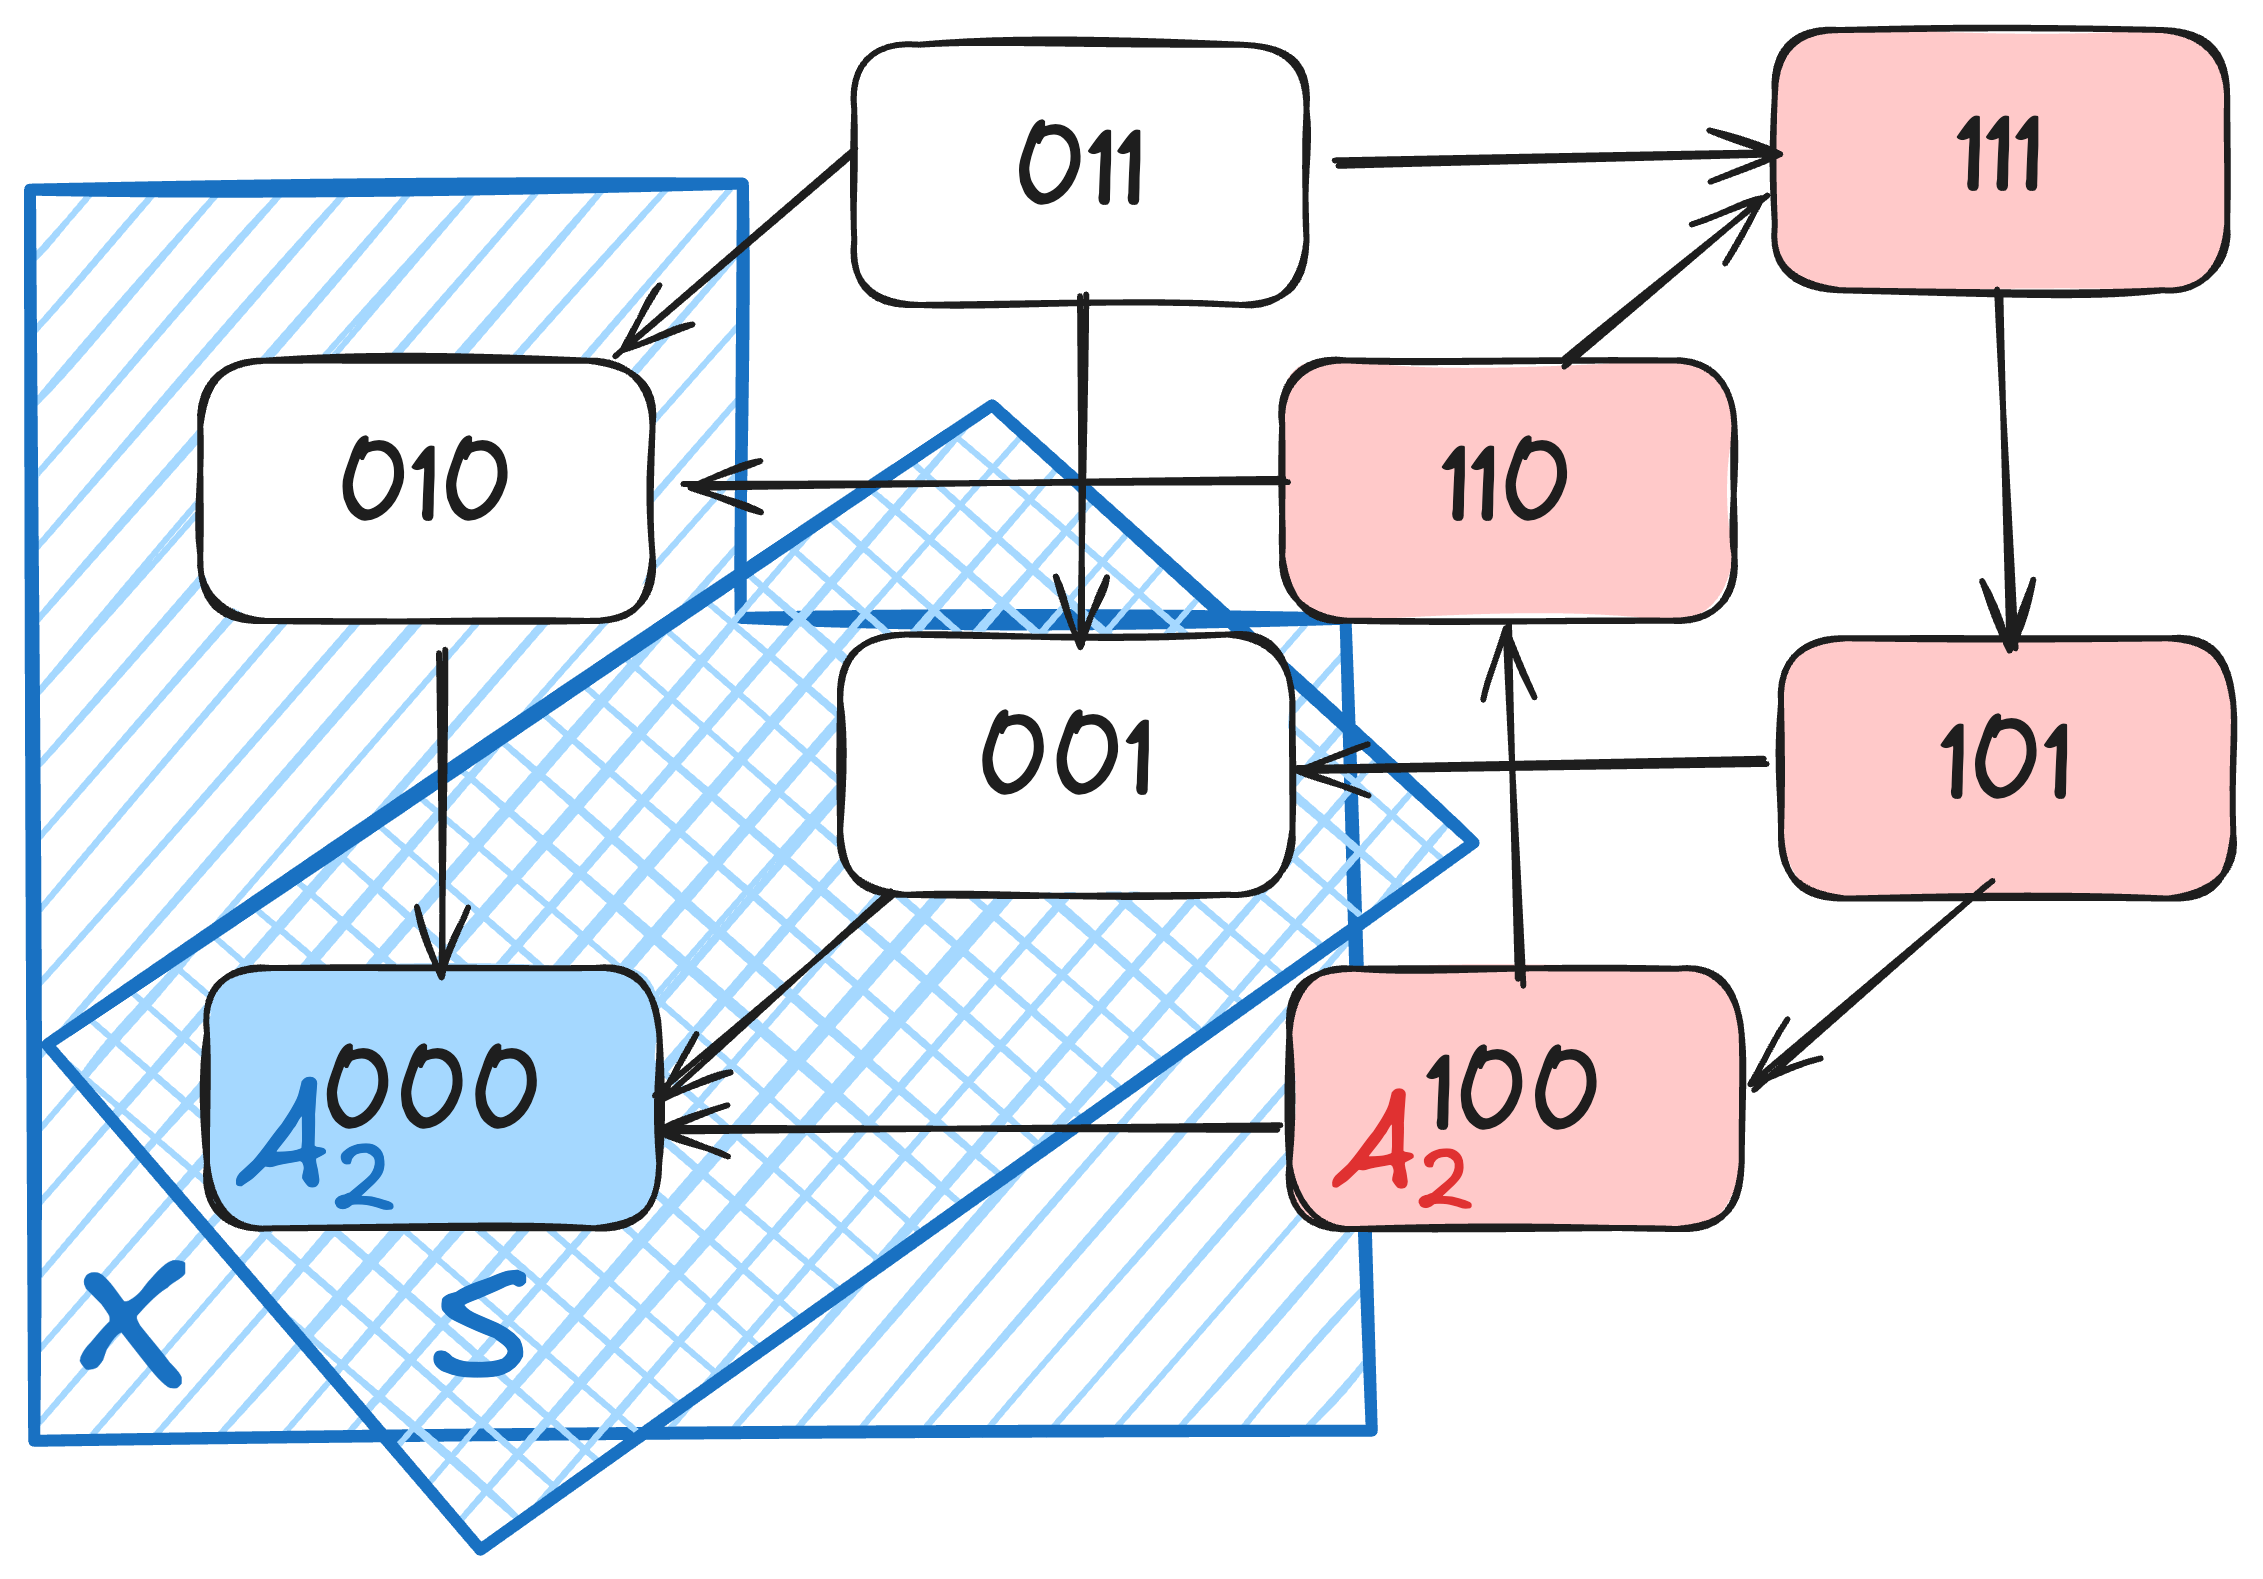
\includegraphics[width=0.4\textwidth]{Figures/traps.png}
    \caption{
        \textbf{Difference between a trap set and a trap space.} A state space of a BN with $n=3$ is shown. The BN contains two attractors: a steady state $A_1$ (a blue state 000) and an oscillatory attractor $A_2$ (red states $1\unspecified\unspecified$). The trap set $S$ (double-shaded are) is also a trap space as it can be described by a subspace $00\unspecified$. On the other hand, the trap set $X$ (shaded area) is not a trap space as it cannot be described by a subspace. Notice, that also a set of all states $\unspecified\unspecified\unspecified$ is a trap space (set), even though it contains multiple attractors.
    }
    \label{fig:traps}
\end{figure}

% \intention{Attractors} 
For a visualization of the concepts, see \autoref{fig:traps}. Equivalently, we can define an attractor $A$ as the inclusion-minimal trap set of $\bnMath$. 

Notice, that an attractor of a run is exactly the set of states that appear infinitely often in the run $inf(\run) = A$. We write $\allAttractors(\STG(\bnMath))$ to denote the set of all attractors of $\bnMath$. An attractor containing only a single state is called a \emph{steady state} or \emph{fixed point}. On the other hand, we will refer to attractors containing multiple states as \emph{oscillatory attractors}*. \marginpar{*Some works also distinguish oscillatory (where period of states repeating in the sequence is strictly regular) and chaotic attractors~\cite{Pastva2022}. In this work we call both these types as oscillatory.}

Finally, observe that due to our fairness assumption, all runs admitted by $\STG(\bnMath)$ eventually reach some attractor. As such, for each strongly fair $\pi$, the set of states that appear infinitely often in $\pi$ is always an attractor. For example, if we consider the BN from \autoref{fig:bn_basic}, it has a single attractor; the oscillation in subspace $0\unspecified\unspecified$. All runs of this BN eventually reach this attractor.

% \textcolor{red}{Basins, weak basin, strong basin}
Given an attractor, we also define its \emph{basin of attraction} as the set of all states that can reach the attractor. The larger the basin of attraction, the attractor is more likely to be biologically relevant~\cite{Klemm2005}. Due to the non-deterministic nature of asynchronous BNs, individual states may reach multiple attractors depending on the selected successor states. To that end, we recognize two types of basins of attraction~\cite{Klarner2018,Schwab2020}:

\begin{definition}
    \label{def:basins}
    The \emph{weak basin of attraction} comprises all states which can lead to the given attractor: 
    $$\weakBasin{\bnMath, \attractor} = \{ x \in \bools^n \mid \exists \run \in \allRuns(\bnMath): x \in \run \land (\forall s \in \attractor : s \in \run) \}$$

    In contrast, the \emph{strong basin of attraction} includes all states from which the given attractor is eventually surely reached.
    $$\strongBasin{\bnMath, \attractor} = \{ x \in \bools^n \mid \forall \run \in \allRuns(\bnMath): x \in \run \Rightarrow (\forall s \in \attractor : s \in \run) \}$$
\end{definition}

If Boolean network $\bnMath$ is clear from the context, it can be omitted from the notation. States which belong to a strong basin of attraction lead to only one possible attractor. In contrast, states in the weak basin of attractor may lead to a certain attractor but also another one. This concept is also shown in \autoref{fig:basins}. As we will see later in \autoref{chapter:source_target_control}, these notions are particularly useful in the context of BN control.

\begin{figure}[bth]
    \centering
    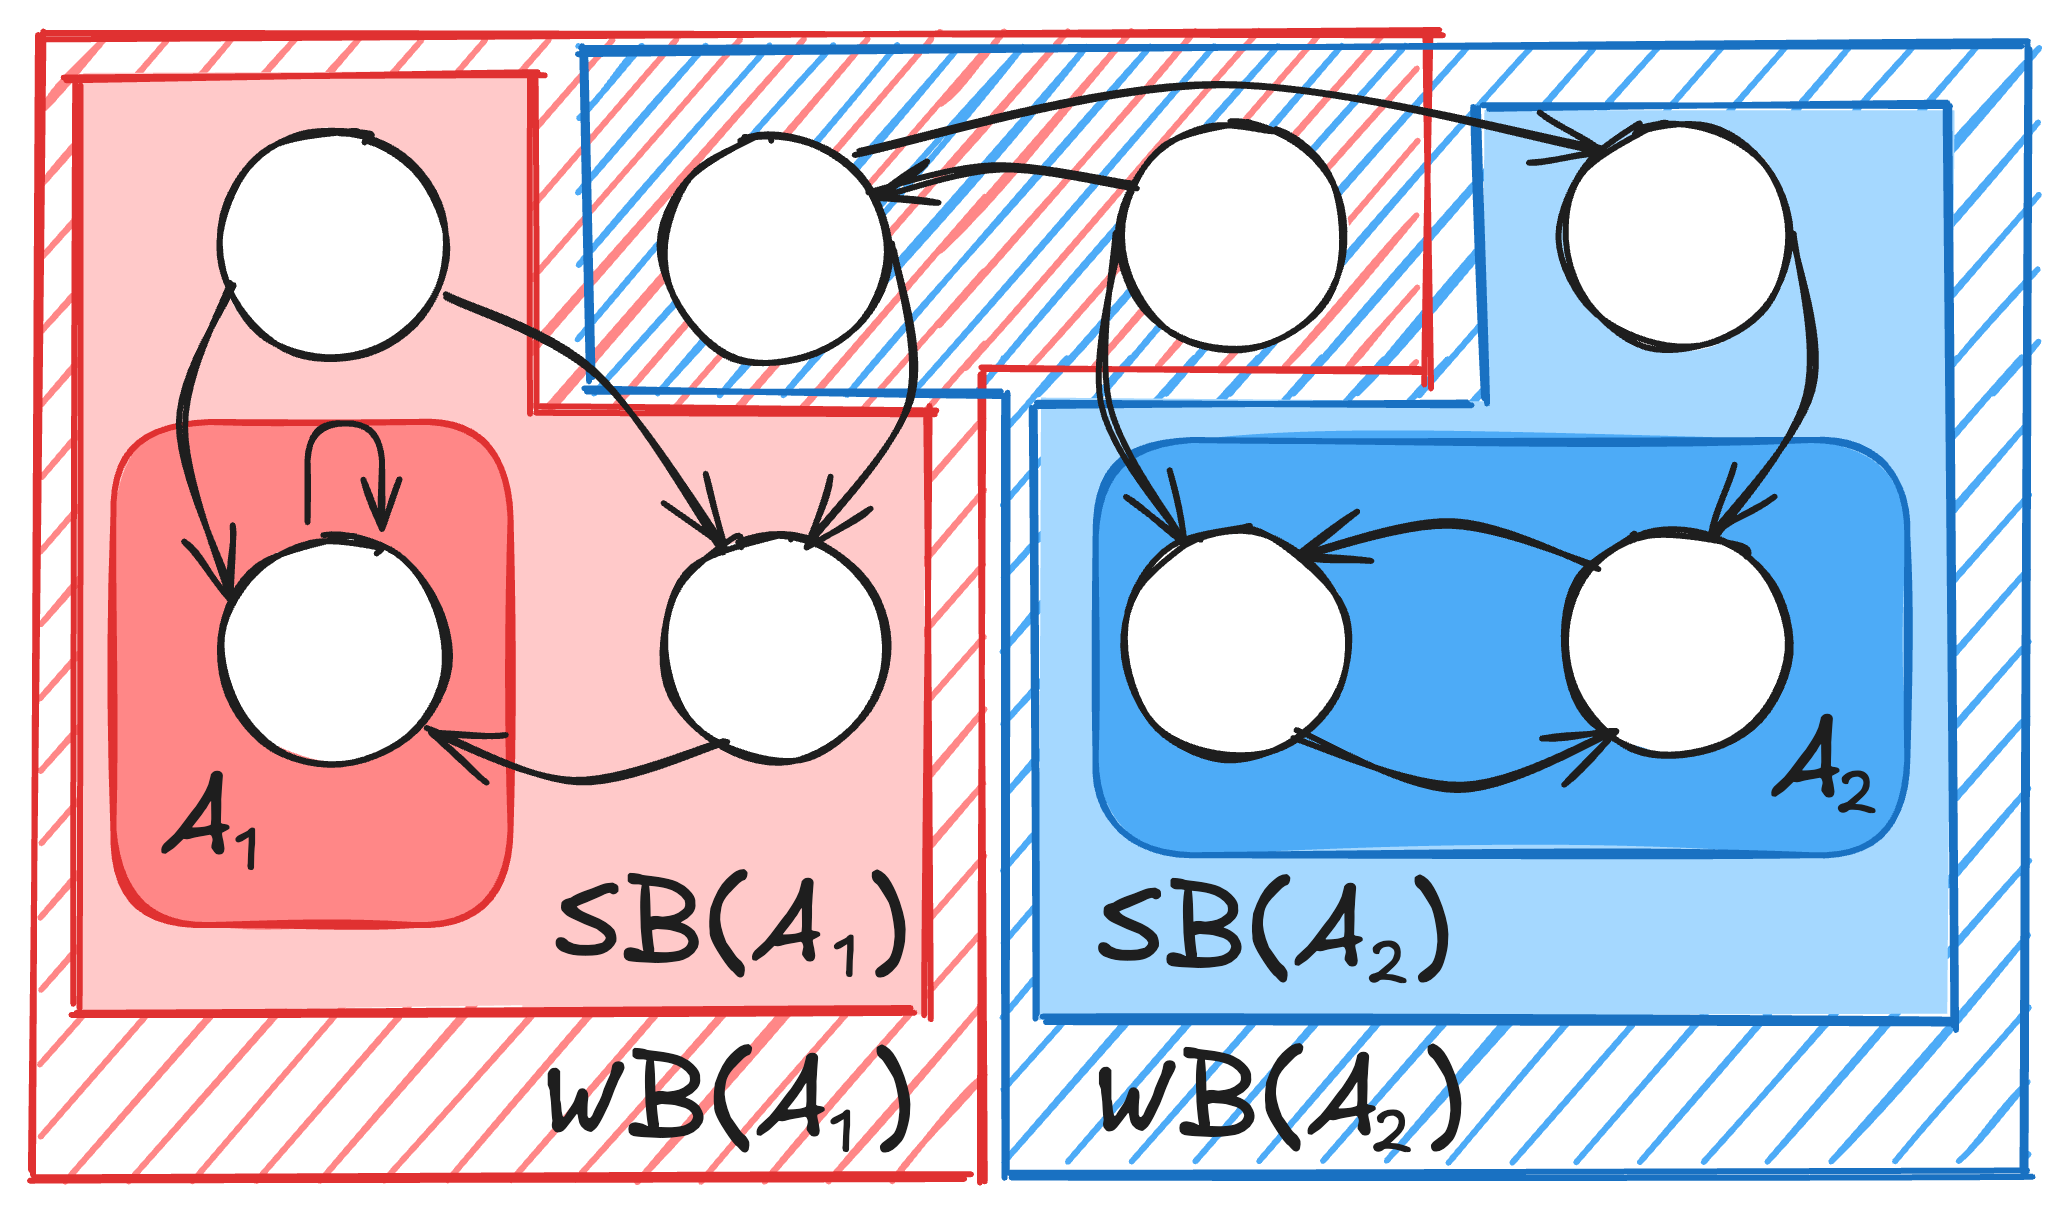
\includegraphics[width=0.8\textwidth]{Figures/basins.png}
    \caption{
        \textbf{Difference between a strong and a weak basin.} The figure shows a simple STG with two attractors: a steady state $A_1$ (dark red) and an oscillatory attractor $A_2$ (dark blue). Strong basins of $A_1$ and $A_2$ are shown in light red and light blue, respectively and are disjoint. Finally, the weak basin of $A_1$ and $A_2$ are shown in red and blue stripes, respectively. The weak basins overlap as some states can reach multiple attractors.
    }
    \label{fig:basins}
\end{figure}

\subsection{Summary}

In this section, we summarized the key concepts related to Boolean networks and their dynamics. We introduced the notions of states and updating schemas. We have introduced state space structures, such as trap sets and attractors, which are crucial for understanding the long-term behavior of Boolean networks Building on these concepts, we now turn our attention to the control of Boolean networks.

\section{Control of Boolean networks}
\label{s:control_of_bns}
\marginpar{
    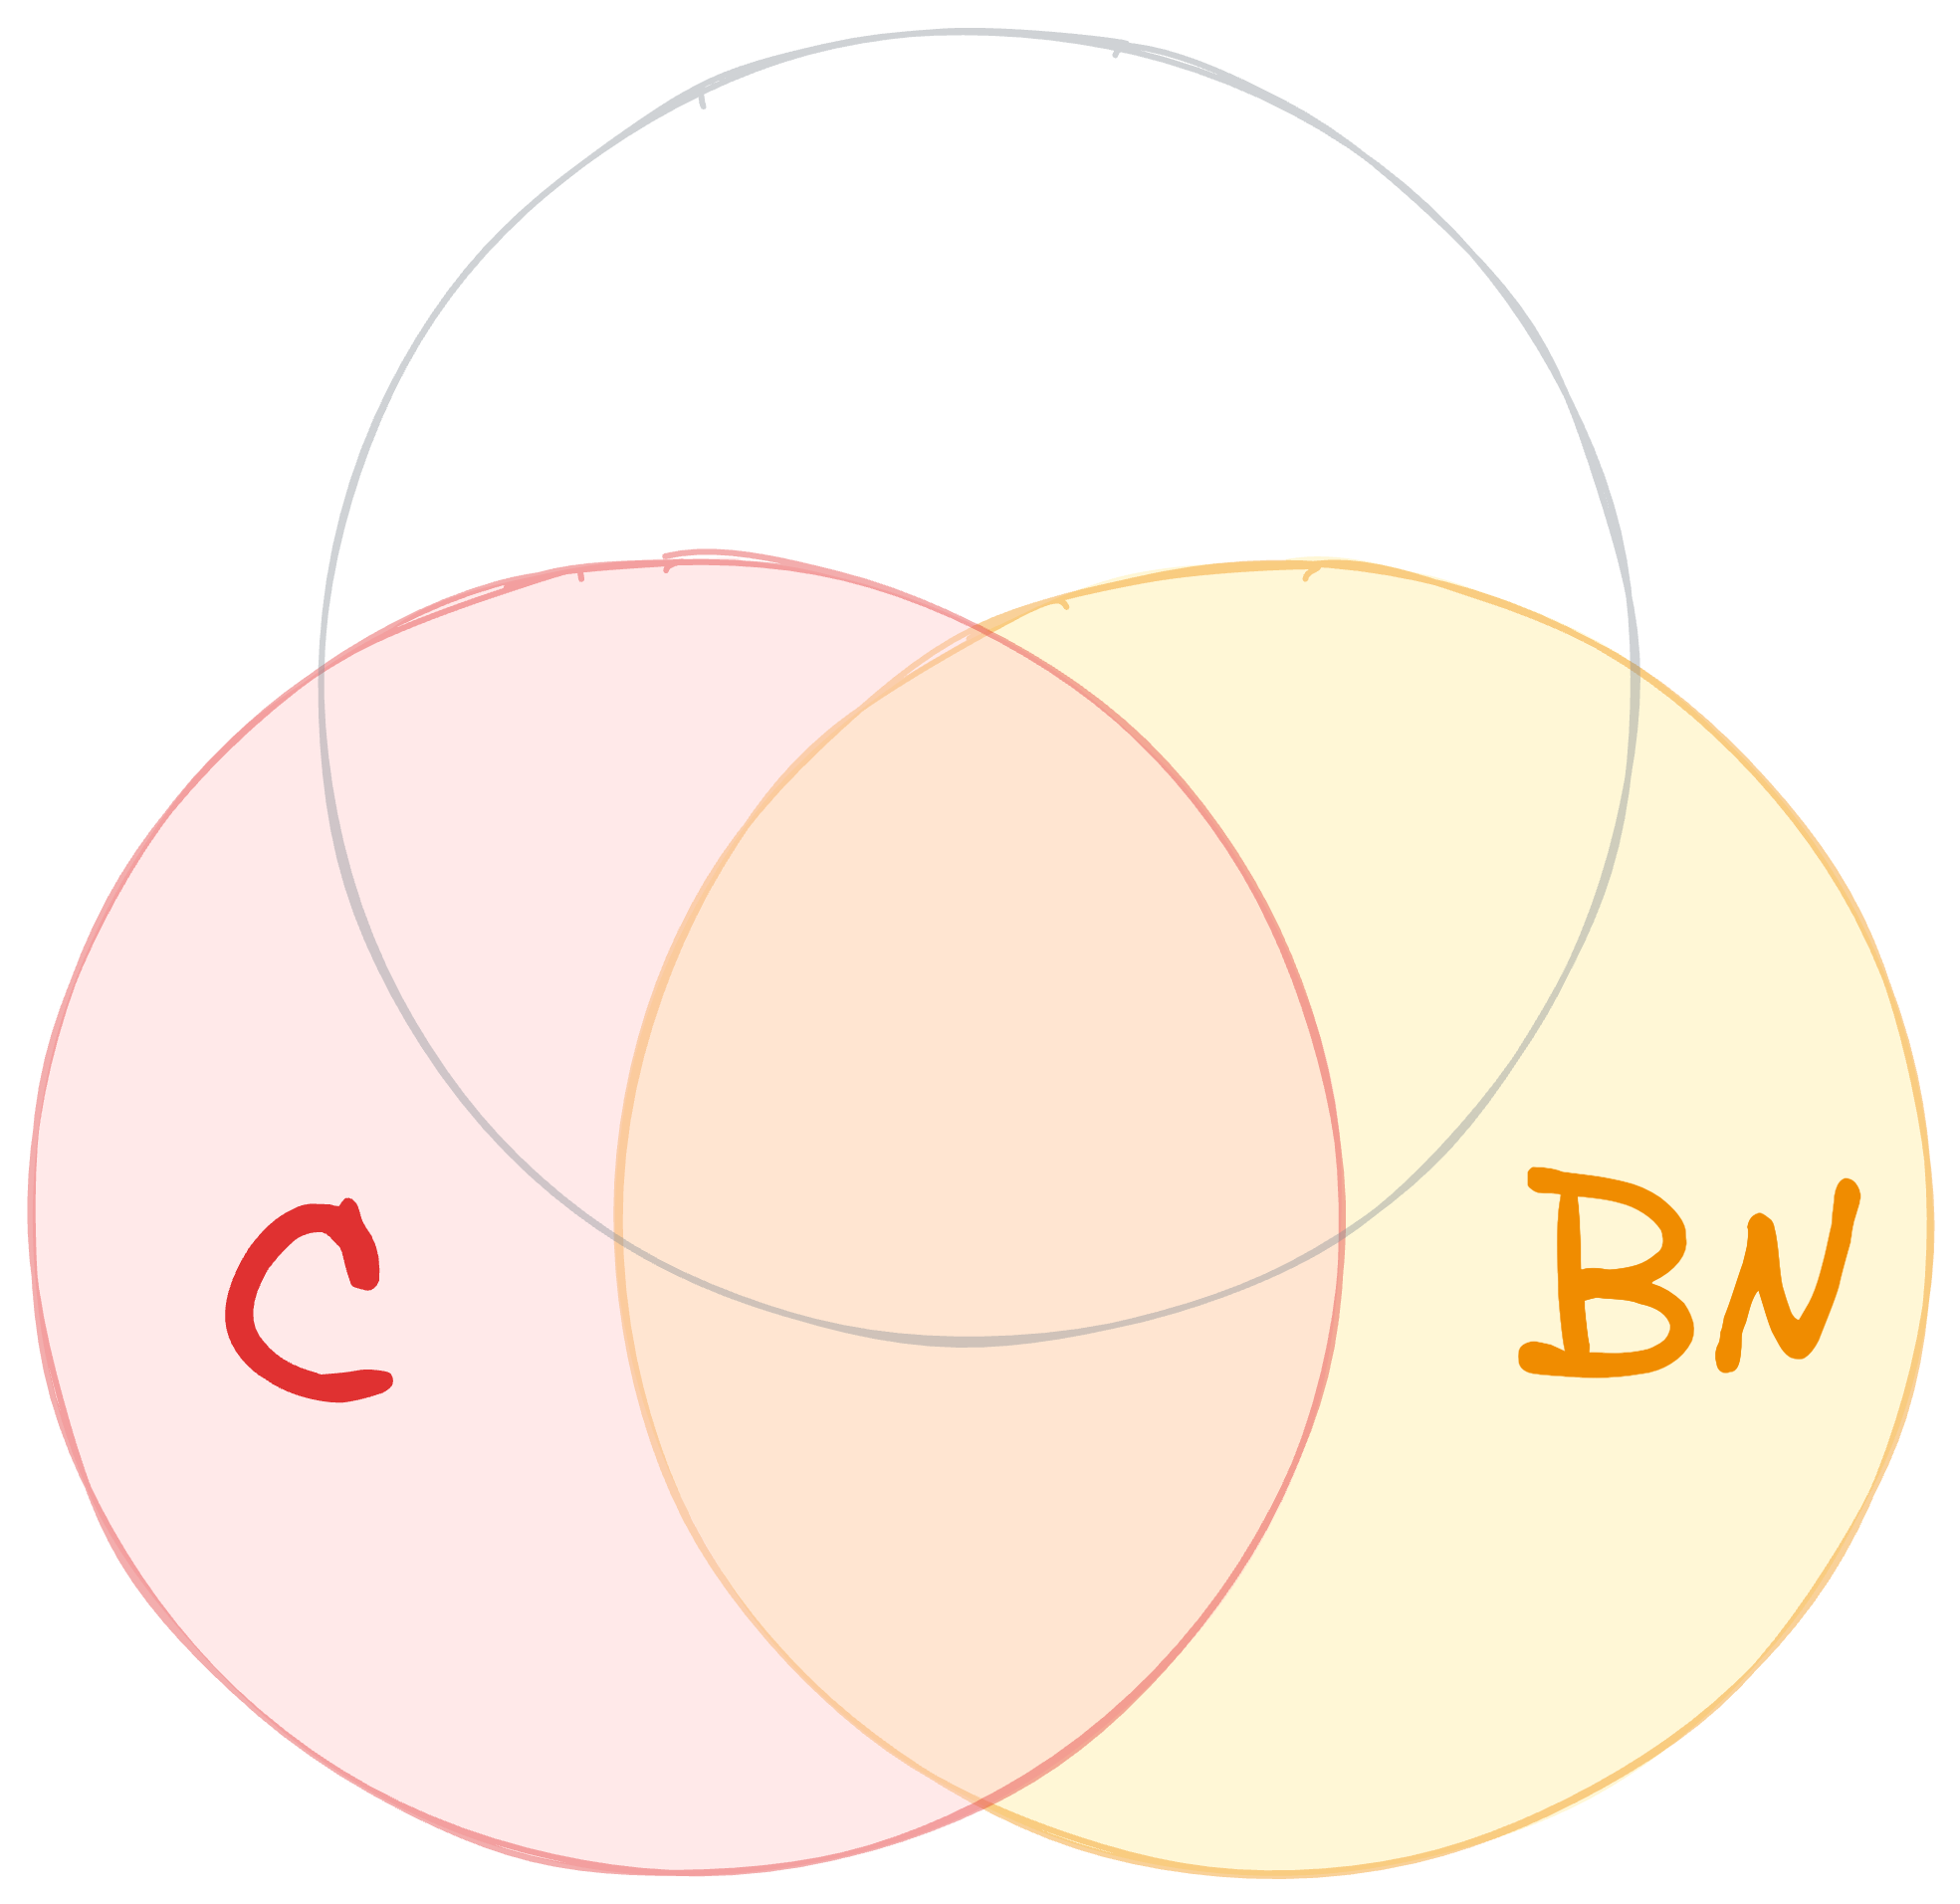
\includegraphics[width=\marginparwidth]{Figures/topics_ctrl_bn.png}
}


In this section we zoom into the \emph{control} of Boolean networks. We first discuss different control objectives that have been studied in the literature. Then, we introduce the concept of perturbations, which are the means of controlling a Boolean network. Finally, we summarize the aspects in which the problem of control of Boolean networks differ.

\subsection{Control objective} \label{sss:controlObj}

% Source-target, target, full control, all pair
The first aspect in which control problems differ is ``what kind of stabilization we are trying to achieve''. Since the only component stable in a BN are its attractors, the control objectives typically focus on navigating a system to reach a certain attractor or a set of attractors.

There are two base types of control objectives: \emph{existential} and \emph{inevitable} control~\cite{Paul2018SETTA,Mandon2019PHD}. Existential control aims to find a strategy that make for a system \emph{possible} to reach the target. On the other hand, universal control seeks a strategy that \emph{ensures} convergence to the target attractor from any initial state. In this work, we consider only the inevitable control objectives.

We consider five different control objectives based on the previous lines of research~\cite{Baudin2019,Fontanals2020}. The differences between control objectives are also illustrated in \autoref{fig:st}:

\begin{enumerate}
\item \emph{Source-target control}: Given a \emph{source state} $s \in \bools^n$, and a \emph{target attractor} $T \in \allAttractors$, ensure, that the BN converges from the state $s$ to the attractor $T$ (see \autoref{subfig:st_a}).
\item \emph{Target control}: Given a \emph{target attractor} $T \in \allAttractors$, ensure that for \emph{any} initial state $s \in \bools^n$ the BN converges from $s$ to $T$ (see \autoref{subfig:st_b}).
\item \emph{Full control}: Find a set of control strategies such that for all pairs of distinct attractors $S, T \in \allAttractors$, applying a strategy from this set guarantees that the BN converges from $S$ to $T$ (see \autoref{subfig:st_c}).
\item \emph{All-pairs control}: Given a subset of source attractors $\mathcal{S} \subseteq \allAttractors$ and target attractors $\mathcal{T} \subseteq \allAttractors$, find a set of perturbations such that for every pair $S \in \mathcal{S}$ and $T \in \mathcal{T}$, applying a subset of the perturbations guarantees that the BN converges from $S$ to $T$ (similar to full control in~\autoref{subfig:st_c}).
\item \emph{Phenotype control}: Given a subset of states $X \subseteq \bools^n$, ensure that from any initial state, the BN converges to an attractor $A \subseteq \allAttractors$ such that $A \subseteq X$ (\autoref{subfig:st_d}).
\end{enumerate}


\begin{figure}[htb]
    \centering
    \subfloat[Source-target control]{
        \label{subfig:st_a}
        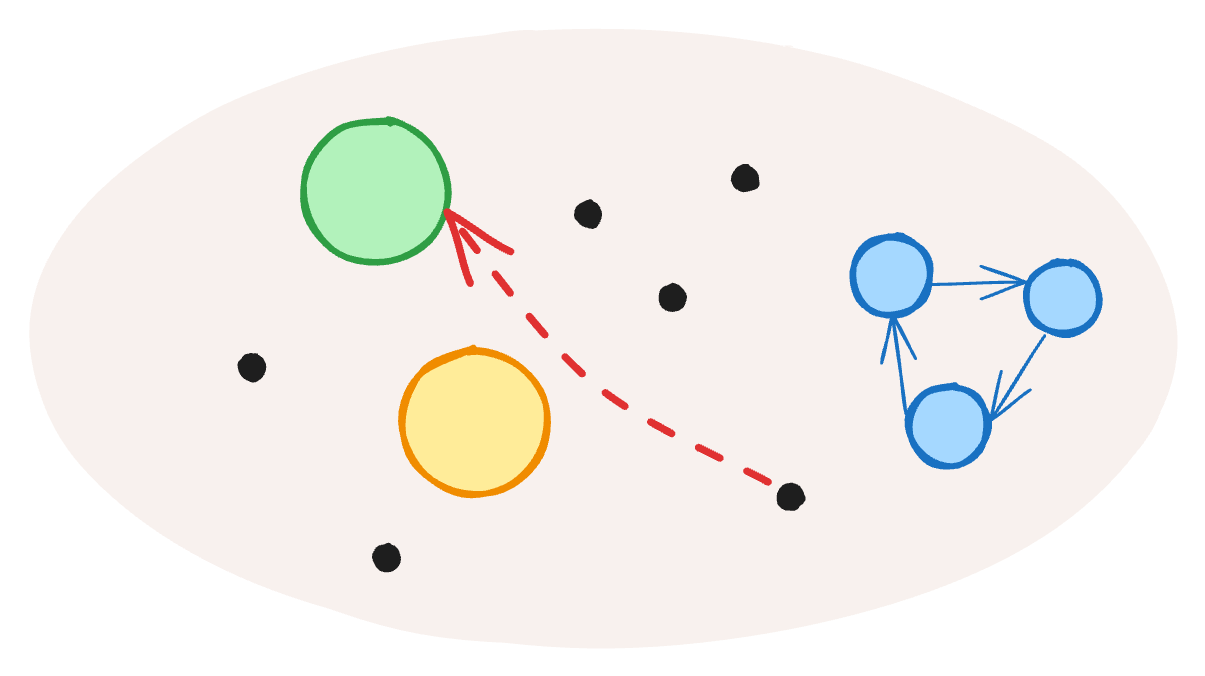
\includegraphics[width=0.4\textwidth,valign=b]{Figures/st_a.png}
    }
    \subfloat[Target control]{
        \label{subfig:st_b}
        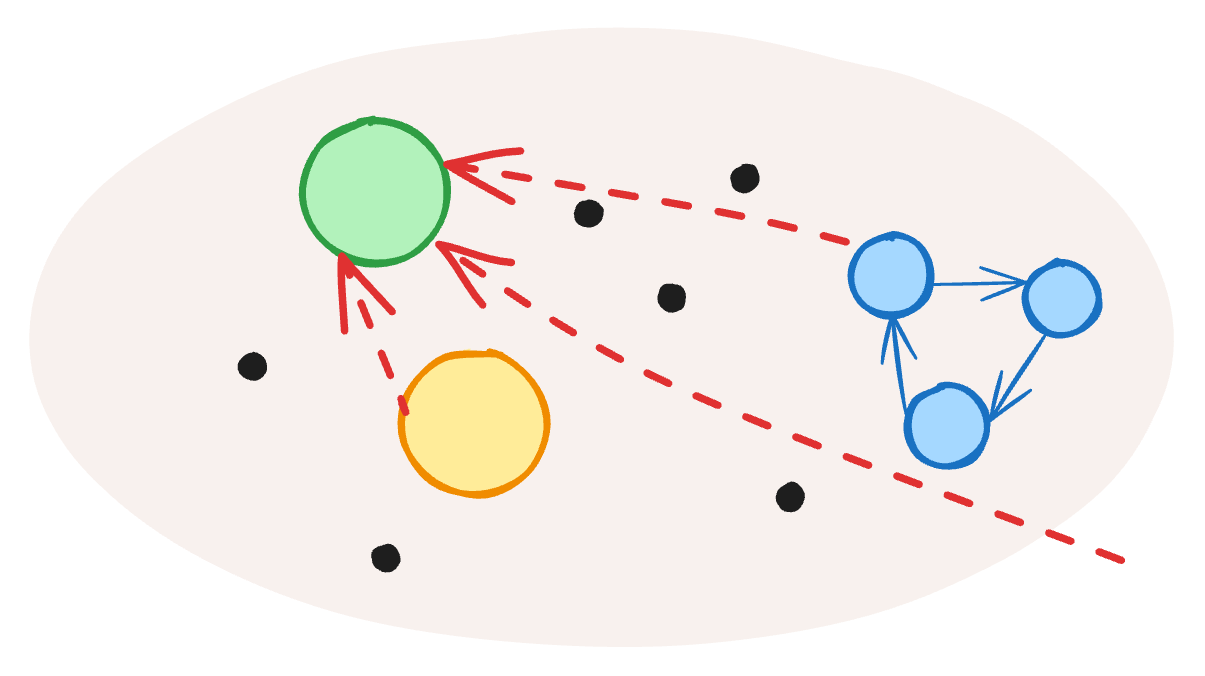
\includegraphics[width=0.4\textwidth,valign=b]{Figures/st_b.png}
    }
    \newline
    \subfloat[Full control]{
        \label{subfig:st_c}
        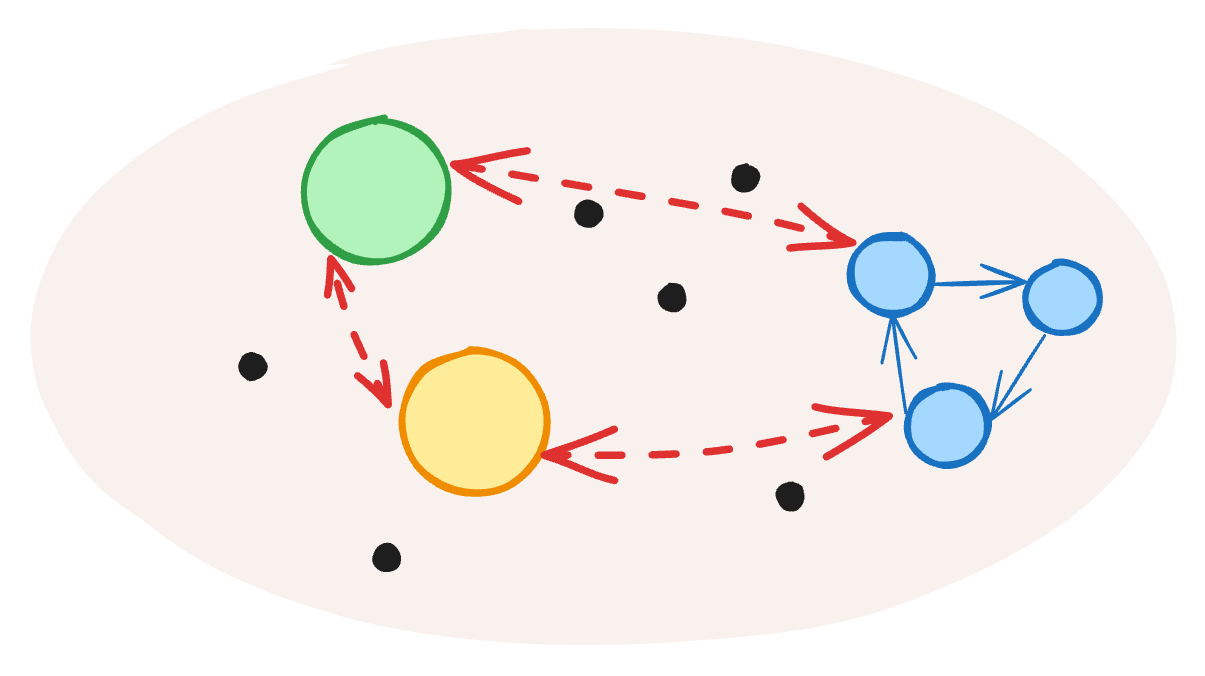
\includegraphics[width=0.4\textwidth,valign=b]{Figures/st_c.png}
    }
    \subfloat[Phenotype control]{
        \label{subfig:st_d}
        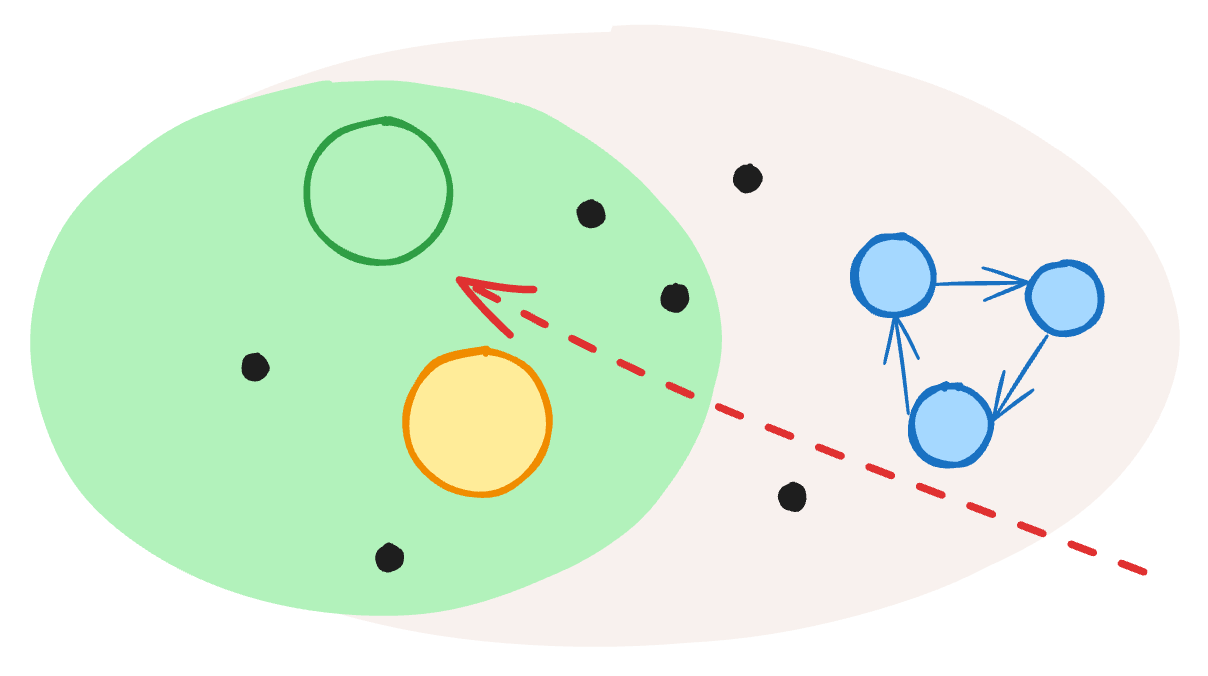
\includegraphics[width=0.4\textwidth,valign=b]{Figures/st_d.png}
    }
    \caption{\textbf{Difference between control objectives.} The black points are non-attractor states of BN, the colorful points are attractors, and the red arrows shows where we are trying to stabilize by applying the control. The green area in the \autoref{subfig:st_d} represents a target phenotype.} 
    \label{fig:st}
\end{figure}


The control objectives as defined above are rather high-level since they do not specify using what means are allowed to achieve the goals. In particular, they do not clarify what types of perturbations can be applied to the system in order to guide it towards the desired attractors. Therefore, we discuss the perturbations next.

\subsection{Perturbations}
\label{subsec:perturbations}
% Explain perturbations and their types
\emph{Perturbations} are the means of controlling a Boolean network. In order to ensure that a network always reaches some attractor which it does not reach in some of its normal runs, logically, we need to interfere with the system in some way. This is exactly what perturbations are -- a forced intervention to the dynamics of a system. There are several types of perturbations, but in this work we focus on \emph{variable perturbations}, which override the value of some variables in the network by constant values. 

Other types of perturbations are \emph{function perturbations} which can override the update functions completely and in a more complex way. However, due to their complexity, they were so far considered only within a context of synchronous Boolean networks~\cite{Liu2017, Xiao2007}. Somewhat less abstract is a concept of \emph{edge perturbations} which can disable or enable certain regulations in the network~\cite{Fontanals2022c}. Both these two notions can be considered within the framework of partially specified Boolean networks, however due to their complexity both in regard to formalization and practical application, they were not included in this work, and we leave their exploration for future research.

The perturbations are formally defined as follows:

\begin{definition}
\label{def:perturbation}
Given a Boolean network $\bnMath = \{f_1, \dots, f_n \}$, a \emph{variable perturbation} is a vector $\perturbation \in \bools_\unspecified^n$. For every $\perturbation_i = \unspecified$, we say that the $i$-th variable is \emph{unperturbed}, whereas for $\perturbation_i = 0$ or $\perturbation_i = 1$, we say that the variable is \emph{perturbed} (to either $0$ or $1$). The \emph{size} of $\perturbation$ is the number of perturbed variables: $\size(\perturbation) = \; \mid \{ i \mid \perturbation_i \neq \unspecified \} \mid$. A perturbation can again be seen as a \emph{subspace} of the $\bnMath$ state space $\bools^n$. The set of all considered perturbations is denoted as $\allPerturbations$ and typically equals to $\bools_\unspecified^n$. 
\end{definition}

We further recognize two special types of perturbations based on their size; an \emph{empty perturbation} is a perturbation of size $0$ (i.e., $\perturbation = \unspecified\unspecified\ldots\unspecified$) which does not perturb any variable, for short, denoted as \emptyPerturbation. In contrast, a \emph{trivial perturbation} is a perturbation of size $n$ (i.e., $\perturbation \in \bools^n$) which perturbs all variables in the network to a value of the target state. Finally, if a perturbation is very small (i.e one or two being perturbed), we can denote it as an assignment of perturbed variables instead of a full vector. For example, for $n=4$, instead of writing $\perturbation = 1\unspecified0\unspecified$, we can write $\{ \var{v1}=1, \var{v3}=0 \}$.

Usually, the perturbations are expensive. Therefore, we want to keep the amount of performed perturbations as small as possible. Thus, control is an optimization problem and is typically measured by a perturbation size (number of perturbed variables), but other criteria might be considered as well.

It can be seen, that the definition of perturbation is rather abstract and does not specify how the perturbation is applied. To make perturbations applicable, we need to consider also \emph{temporal} properties of perturbations.

\subsection{Temporal properties of perturbations}
% \intention{Single-step, temporary, permanent perturbations} 
The perturbations differ based on their temporal characteristics. The first classification is based on the length of the applied perturbation. We consider \emph{one-step}, \emph{temporary}, and \emph{permanent} perturbations. \autoref{fig:otpc} shows an intuition on the differences between these types of perturbations. 

\begin{figure}[bth]
    \centering
    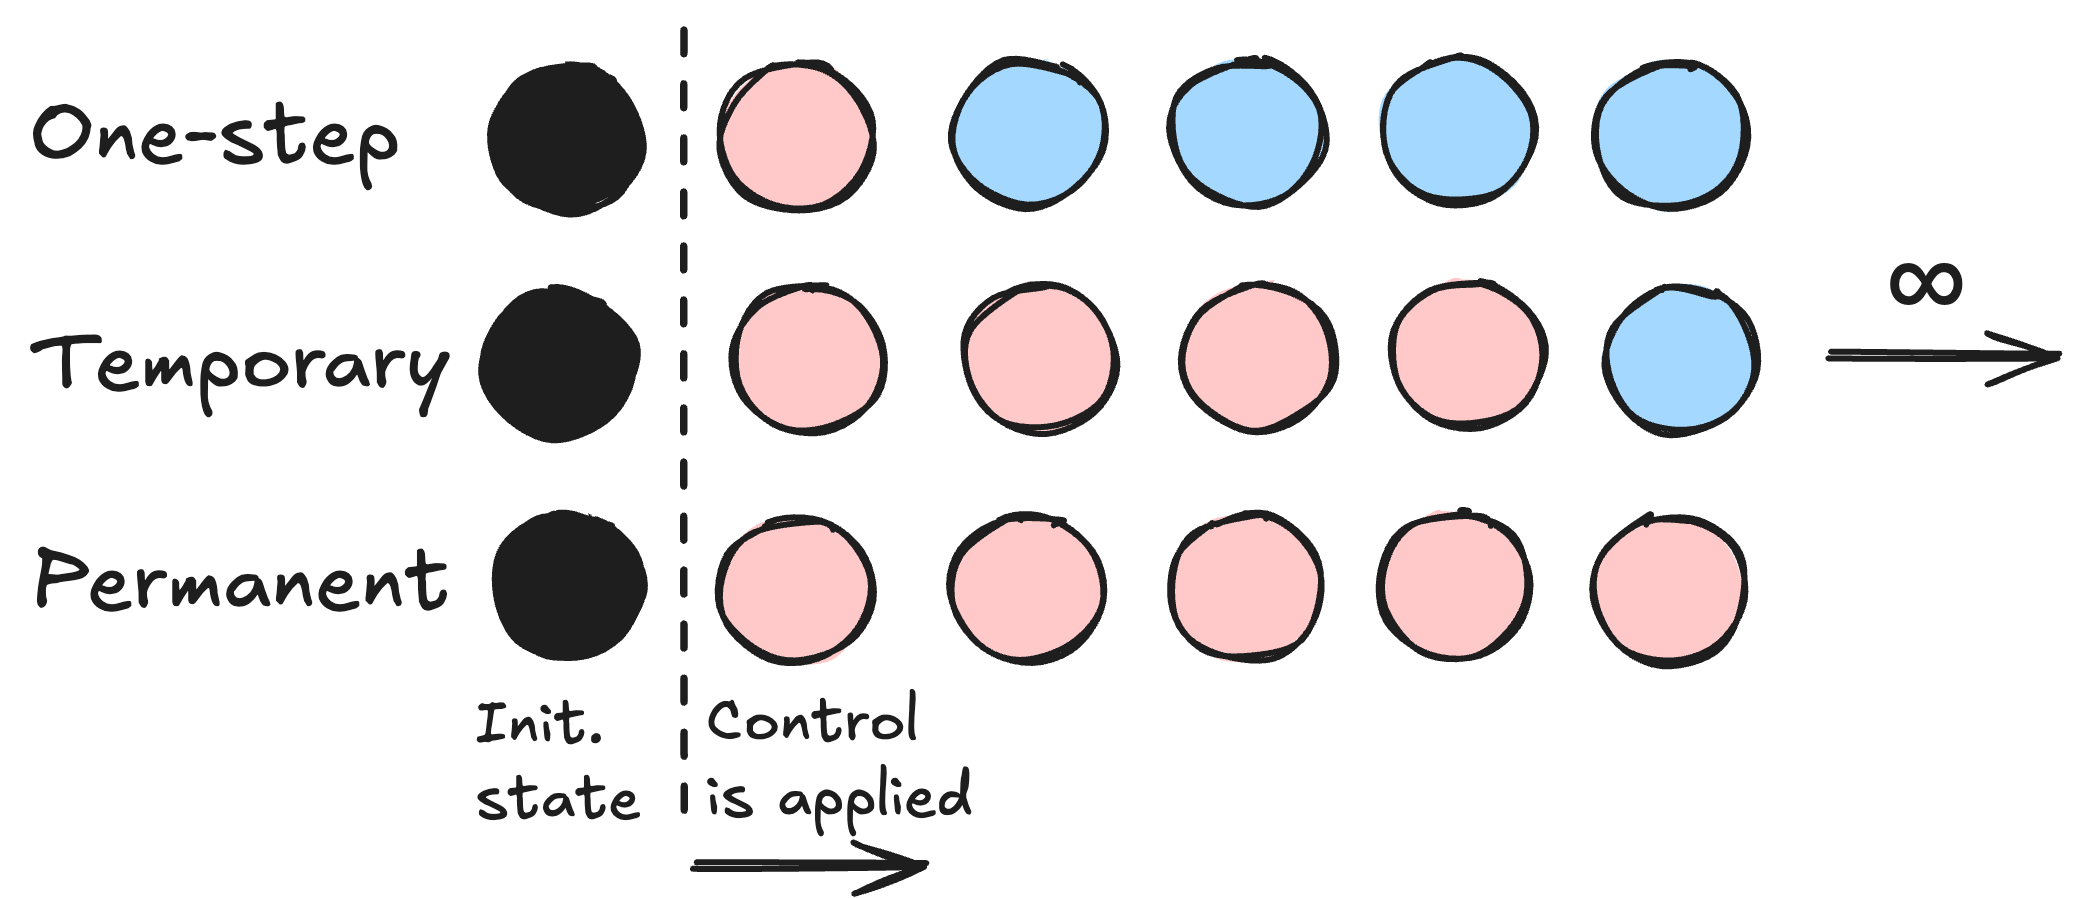
\includegraphics[width=0.8\textwidth]{Figures/otpc.png}
    \caption{
        \textbf{Difference between one-step, temporary and permanent control.} The black markers represent initial states. Red markers represent states which were reached during the time while BN was perturbed and finally, blue markers represent states to which BN transitioned with its natural behavior. The run of BN would continue in the same nature as its last transition.
    }
    \label{fig:otpc}
\end{figure}


\emph{One-step perturbation} (OSP) overrides values of controlled variables once, and then the network is left to evolve in its natural dynamics. Intuitively, the OSP can be viewed as a restriction of the initial states of all BN runs. Technically, the BN run may be at any state before the time step in which the perturbation is applied. Nonetheless, the very next step would bring the network to a state which is part of the OSP. The notion of one-step state perturbation is defined in the following way:

The perturbations applied for multiple time-steps are temporary (TP) and permanent perturbations (PP). As the name suggest, when we use temporary perturbation, there exists a finite amount of time steps after which the perturbation is released, and BN is left to evolve in its natural dynamics. Temporary perturbation applied for only a single time step is equivalent to OSP. 

Finally, the most intrusive perturbations are permanent. This kind of perturbation might be harder to achieve in practice, depending on the specific perturbation context and techniques. Moreover, the permanent perturbation might disrupt the network's original long-term behavior and change the network's attractor landscape; even cause a target attractor to be no longer present in the BN.

To formally define application of perturbations, we differentiate between two types of perturbation applications. The first type is an application to a specific source state, as is the case of source-target control.

\begin{definition}
    \label{def:perturbation_application}
    Given a BN $\bnMath = \{f_1, \ldots, f_n\}$, \emph{application of a perturbation $\perturbation \in \allPerturbations$ to a source state $s \in \bools^n$} is a \emph{forced} state transition (i.e., might not follow the BN standard dynamics), $\pertApply(s, \perturbation) = s \to s'$ such that: 
    $$\pertApply(s_i, \perturbation) = s'_i = \begin{cases}
        s_i & \text{iff } Q_i = \unspecified \\
        Q_i & \text{iff } Q_i \neq \unspecified
    \end{cases}$$
    where $s'$ is the state reached after applying the perturbation.
\end{definition}

After application of a perturbation to a state*\marginpar{*What we call here an application of perturbation (\pertApply) is in some literature called state perturbations and a perturbed BN or runs of perturbed BN are referred to as function perturbations~\cite{Mandon2019PHD}. This is because constants are seen to be an override of variable update function. However, we avoid function perturbation term to avoid confusion with line of work on synchronous Boolean networks where more complex than constant functions are used to perturb networks~\cite{Liu2017}.}, we obtain a state which is \emph{compliant} with the perturbation. This means that the state does not contradict any of the perturbed variables. For example, if we apply perturbation $1\unspecified0$ to state $001$ (contradicting the perturbation at the first variable), we obtain state $101$ which is compliant with the perturbation.

The aforementioned definition is effectively capturing the concept of one-step perturbation for the source-target control. Nonetheless, if we wanted to consider OSP for target or phenotype control, we need to generalize the definition to a whole set of states. To that end, we can adapt the definition above to a set of (all) states and as a result, we obtain a subspace equivalent to the given perturbation as the viable set of initial states.

Another important concept we need to define to understand the application of temporary and permanent perturbations is a \emph{perturbed state transition graph} for a BN:

\begin{definition}
    \label{def:perturbed_stg}
    Given a BN $\bnMath = \{f_1, \ldots, f_n\}$ where $\STG(\bnMath) = (\vertices, \edges)$, \emph{application of a perturbation $\perturbation \in \allPerturbations$ to a Boolean network $\bnMath$} results in a \emph{perturbed Boolean network} $\bnMath_{\perturbation}$ with \emph{perturbed state transition graph} $\STG_{\perturbation}(\bnMath) = (\perturbation, \edges_{\perturbation})$ where vertices are a subspace of the unperturbed state space $\vertices = \bools^n$ given by the perturbation $\perturbation$ and a set of perturbed edges $\edges_{\perturbation} \subseteq \edges$ is given as follows:
    $$
    \edges_{\perturbation} = \{(u, v') \mid (u, v) \in \edges \land u \in Q \land v \in \perturbation\}
    $$
\end{definition}

We can see, that by definition, the perturbed state transition graph is a subgraph of the original state transition graph, containing only the states and transitions that are not violating the perturbation. On the other hand, the perturbed STG might contain different attractors than the original STG. For example trivially, if a BN contains a steady-state attractor, and we apply a perturbation that contradicts some variable of the attractor, the attractor may no longer be present in the perturbed STG. Another example can be seen in \autoref{fig:pert_stg} where due to perturbation the former attractor $1\unspecified\unspecified$ is no longer present and is replaced by the steady-state attractor $110$.

\begin{figure}[bth]
    \centering
    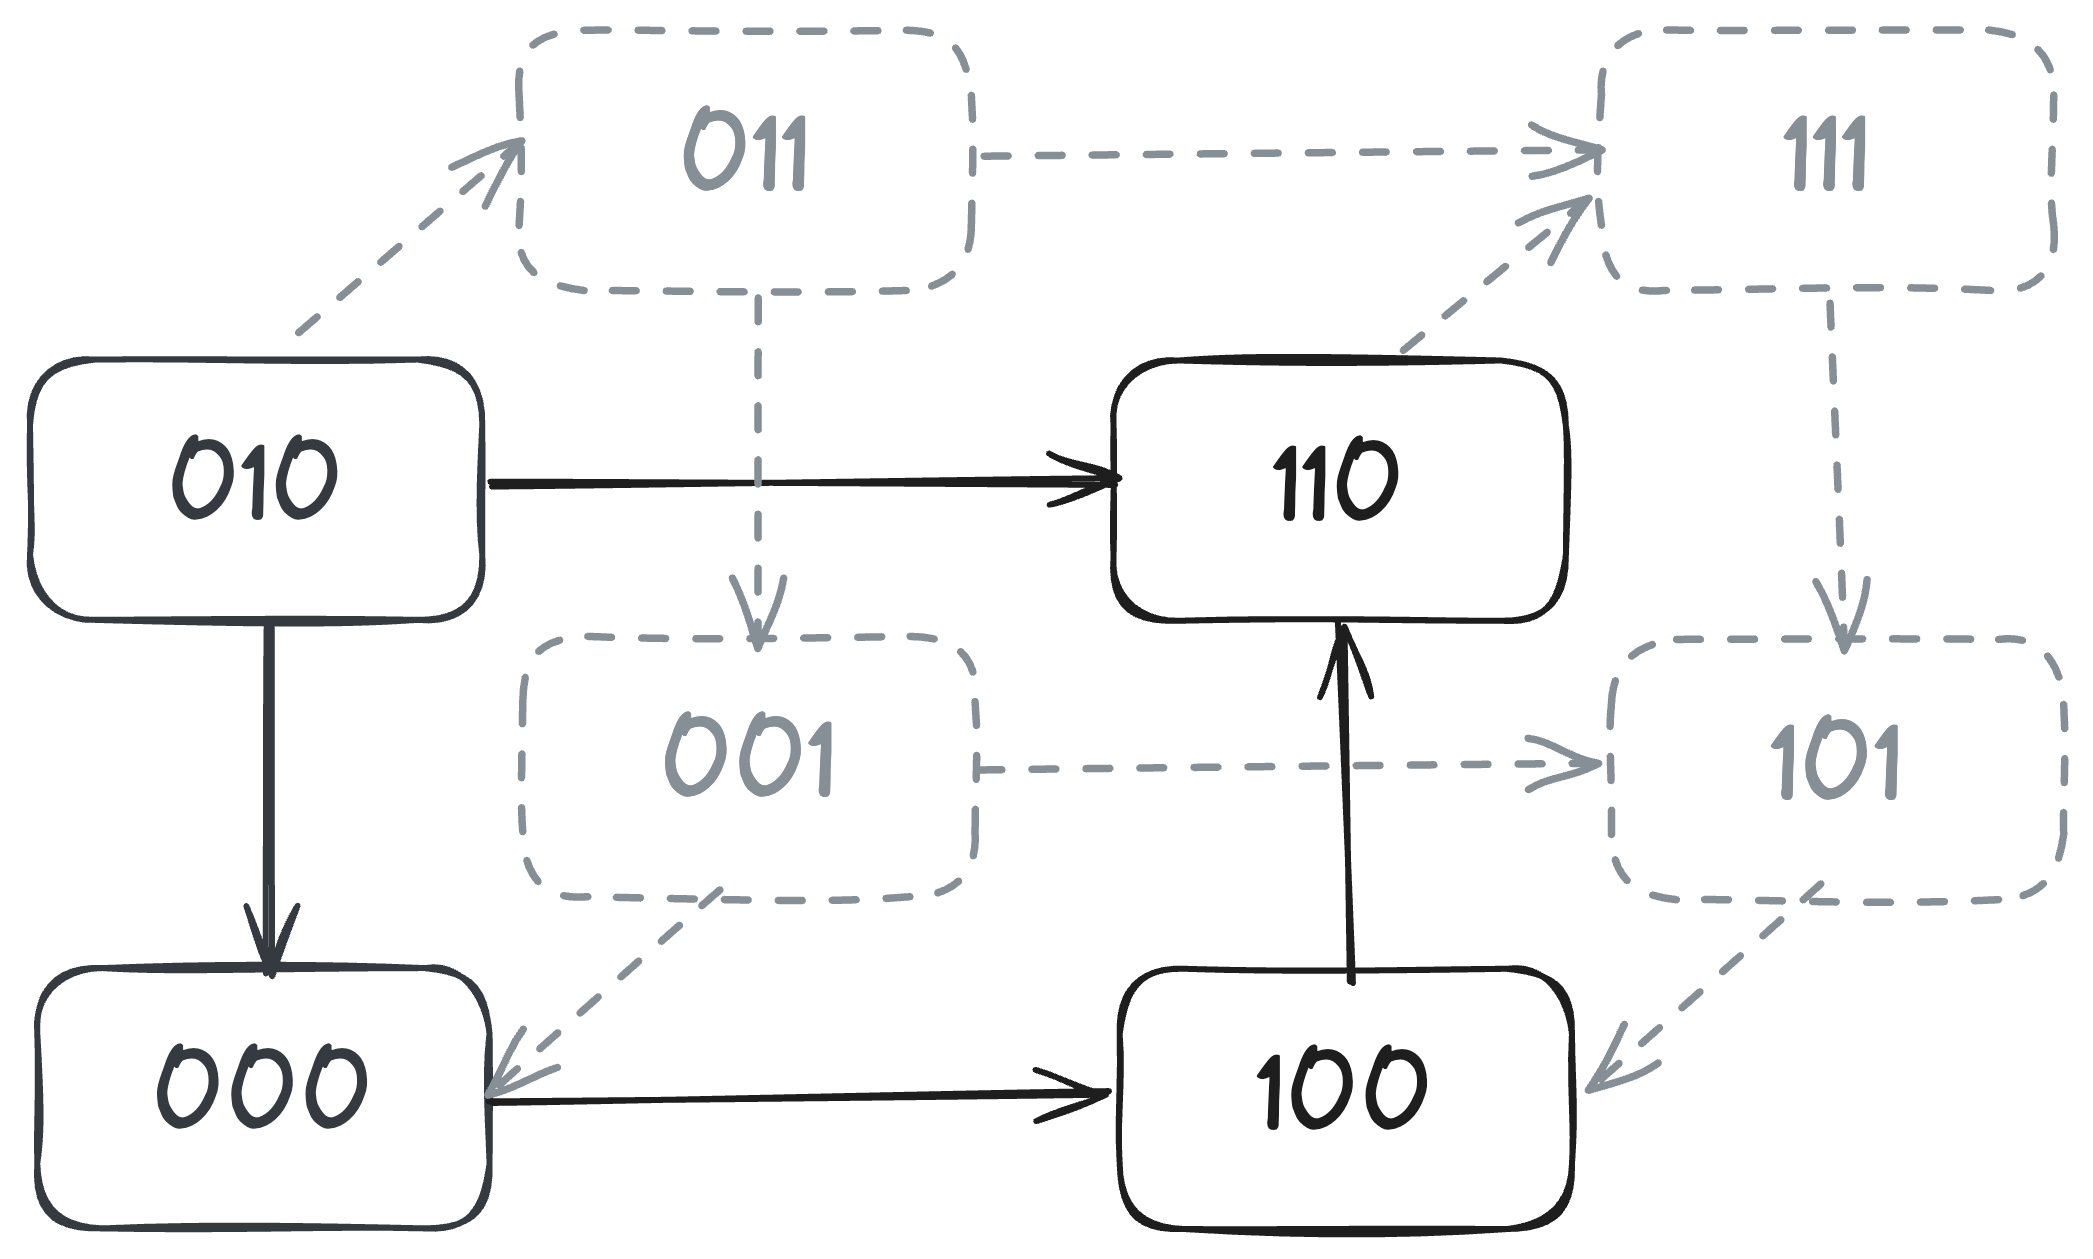
\includegraphics[width=0.45\textwidth]{Figures/perturbed_simple_stg.png}
    \caption{
        \textbf{A perturbed state transition graph of a Boolean network.} The depicted STG is a perturbed version of the STG from \autoref{subfig:stg} under perturbation $\unspecified\unspecified0$. The black solid vertices and edges mark the states and transitions that are preserved in the perturbed STG while the gray dashed vertices and edges represent the states and transitions that have been removed due to not being consistent with the perturbation.}
    \label{fig:pert_stg}
\end{figure}

Now, we can define a perturbed run of a BN:

\begin{definition}
    \label{def:perturbed_run}
    Let us assume a BN $\bnMath = \{f_1, \ldots, f_n\}$, a source states $S \subseteq \bools^n$, a perturbation $\perturbation \in \allPerturbations$, a time period $z \in \Nats_{\infty}$, after which the perturbation is withheld and a natural run $\run \in \STG(\bnMath)$, such that there exists a time-step $t'$ where $\run(t') \in S$. \emph{A perturbed run $\run_{\perturbation}$} is a run which satisfies the following conditions:
    $$
    \run_{\perturbation}(t) = \begin{cases}
        \run(t) & \text{iff } t \leq t' \\
        \pertApply(t, \perturbation) & \text{iff } t = t' + 1 \\
        s'  \text{ s. t. } \run(t-1) = s'' \land (s'', s') \in \edges_{\perturbation} & \text{iff }  t'+z > t > t' + 1 \\
        s'  \text{ s. t. } \run(t-1) = s'' \land (s'', s') \in \edges & \text{iff } t > t'+z
    \end{cases}
    $$
    A set $\allRuns_{\perturbation}(\bnMath, S, z)$ is a collection of all perturbed runs $\run_{\perturbation}$ for a given perturbation $\perturbation$, applied to any state from $S$ with perturbation being withheld after $z$ time-steps.
\end{definition}

 Intuitively, a perturbed run consists of four "stages". First, the run is evolved ``normally" in a given BN. When the BN reaches a state in $S$ (does not need to be the first occurrence of an $s \in S$ in the run), we apply a perturbation to that state. Asz a result, we obtain the nearest state which is compliant with the perturbation. From this state, the BN evolves according to the perturbed STG. If $z$ is not infinite, after $z$ time-steps, the perturbation is withheld, and the BN continues to evolve according to its natural dynamics. 

\begin{example}
An example of a valid perturbed run for a BN from our running example (\autoref{fig:bn_basic}) under perturbation $\unspecified\unspecified0$ applied to a state $101$ and withheld after $z=5$ time-steps is the following:

\begin{itemize}
    \item $t=0 \ldots 2$: The BN evolves naturally, e.g., traverses the states $011 \to 001 \to 101$.
    \item $t=3$: The perturbation $\unspecified\unspecified0$ is applied, resulting in state $100$.
    \item $t=4 \ldots 8$: The BN evolves according to the perturbed STG, reaching state $110$. There are no further viable transitions in the perturbed STG, therefore the BN remains in state $110$.
    \item $t=9$: The perturbation is withheld, and the BN continues to evolve naturally, stabilizing in the attractor $1\unspecified\unspecified$.
\end{itemize}
\end{example}

\begin{table}[htb]
\caption{\textbf{Types of perturbations.} The table summarizes the differences between one-step, temporary, and permanent perturbations when applied to a source-target control, or target types of control (target/full/all-pair/phenotype).}
\begin{tabular}{llll}
 & one-step & temporary & permanent \\
 \hline
source-target & \begin{tabular}[c]{@{}l@{}}$\pertApply(s, \perturbation)$ or\\ $\allRuns_{\perturbation}(\bnMath, \{s\}, 1)$ \end{tabular} & \begin{tabular}[c]{@{}l@{}}$\allRuns_{\perturbation}(\bnMath, \{s\}, z)$\\ s.t. $z \in \Nats$ \end{tabular} & $\allRuns_{\perturbation}(\bnMath, \{s\}, \infty)$\\
\hline
target & \begin{tabular}[c]{@{}l@{}}$\pertApply(\bools^n, \perturbation)$ or\\ $\allRuns_{\perturbation}(\bnMath, \bools^n, 1)$ \end{tabular} & \begin{tabular}[c]{@{}l@{}}$\allRuns_{\perturbation}(\bnMath, \bools^n, z)$\\ s.t. $z \in \Nats$ \end{tabular} & \begin{tabular}[c]{@{}l@{}}$\allRuns_{\perturbation}(\bnMath, \bools^n, \infty)$ or\\ $\bnMath_{\perturbation}$ \end{tabular}
\end{tabular}
\label{tab:perturbation_types}
\end{table}

The \autoref{tab:perturbation_types} summarizes the different types of perturbations and how they can be implemented in the context of different control objectives using the concepts of perturbation application, perturbed STG, and perturbed runs. We can notice, that a one-step control can be seen as a special case of temporary control with time steps sustaining perturbation $z=1$. Moreover, permanent control can be implemented as a perturbed Boolean network.

\begin{figure}[hb!]
    \centering
    \subfloat[Initial perturbation]{
        \label{subfig:ssa_a}
        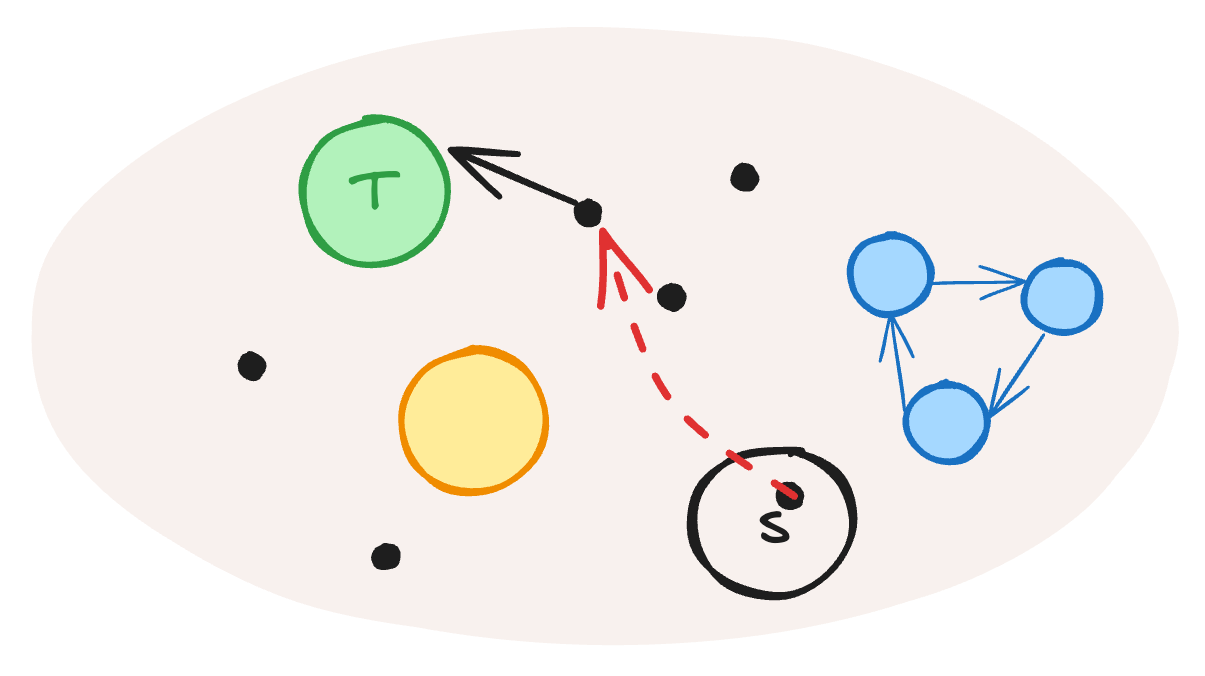
\includegraphics[width=0.4\textwidth,valign=b]{Figures/ssa_a.png}
    }
    \subfloat[Sequential perturbation]{
        \label{subfig:ssa_b}
        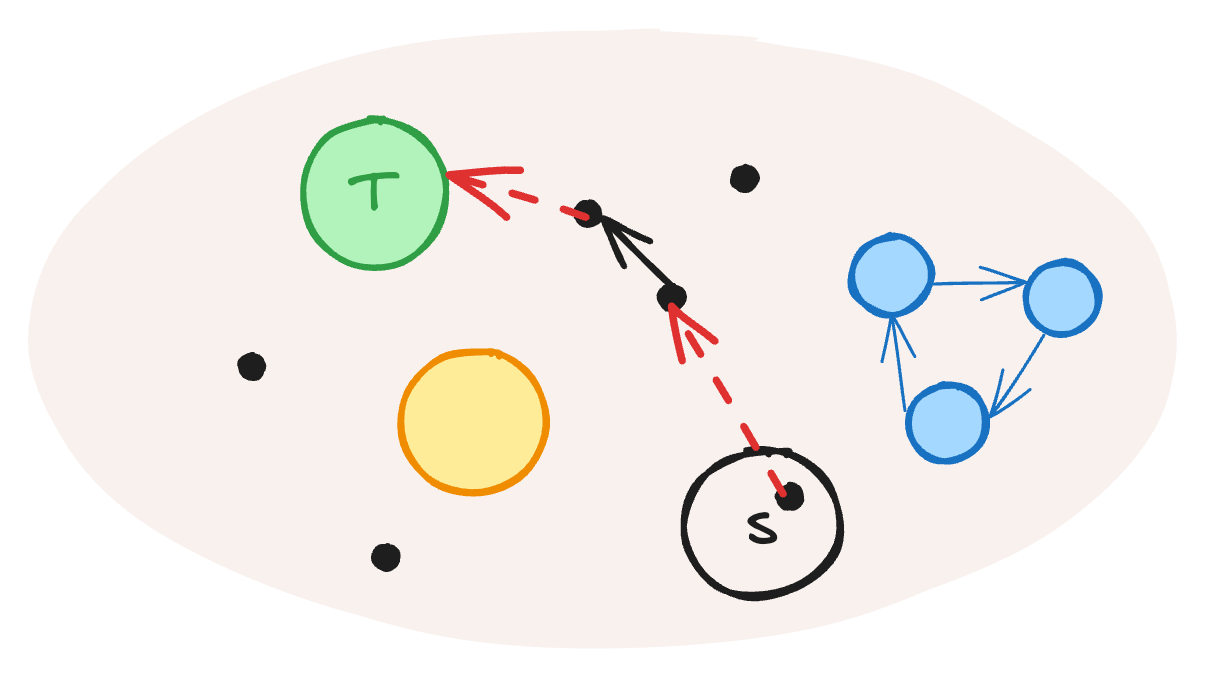
\includegraphics[width=0.4\textwidth,valign=b]{Figures/ssa_b.png}
    }
    \newline
    \subfloat[Sequential attractor-based \newline perturbation]{
        \label{subfig:ssa_c}
        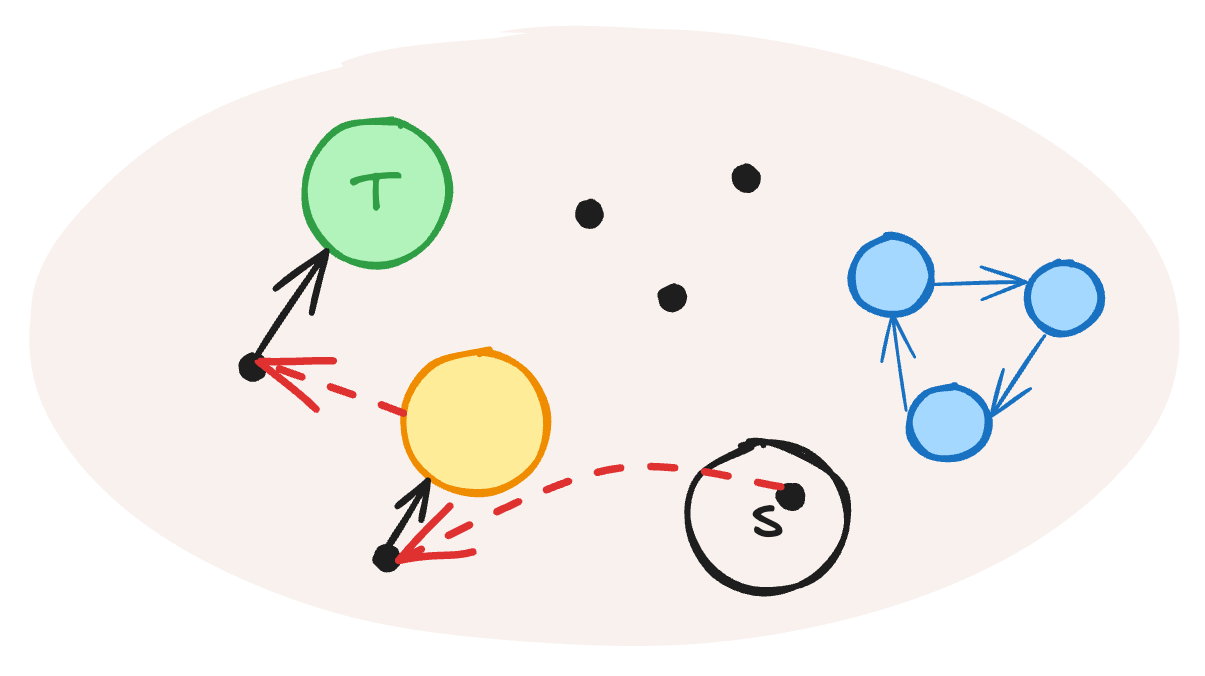
\includegraphics[width=0.4\textwidth,valign=b]{Figures/ssa_c.png}
    }
    \caption{\textbf{Difference between initial, sequential, and sequential attractor-based perturbations.} The figure is only illustrative and does not show precise transitions or perturbations done to the BN. The black points are non-attractor states of BN. The colorful points are attractors, the black arrows are transitions conducted by natural BN dynamics, and the red dashed arrows are transitions done under the effect of perturbations. The initial state is marked as s while the target attractor is the blue one marked with T.} 
    \label{fig:ssa}
\end{figure}

% \intention{Sequential control} 
Some perturbation techniques also consider \emph{when} the perturbations are applied. In \emph{initial} or also referred to as \emph{immediate} control, the perturbations are applied to the given initial state. 

Alternatively, during \emph{sequential} control, (possibly different) perturbations can be applied multiple times at different states. This way, we can potentially control the system using fewer perturbations. However, this approach brings new issues, such as dealing with the non-determinism of the BN (different perturbations may be required for different branches of the non-deterministic network's behavior). 

Moreover, we would need to be able to precisely observe the current state of the BN, which can be very problematic to obtain in practice. These issues can be addressed by using \emph{attractor-based sequential} approach~\cite{Mandon2019CMSB}. Differences between these approaches are depicted in \autoref{fig:ssa}.

In this work, we focus only on the initial control approach, since attractor landscape can be very complex in context of partially specified Boolean networks. On the other hand, the sequential control approach may offer smaller perturbation sizes in certain scenarios that might arise in a future research.

\subsection{Summary}

In summary, the control problems for Boolean networks differ in the following aspects:

\begin{itemize}
\item \emph{What do we want to control; goal}: What is the initial state of the BN? Where we  want to end? Do we want to control only one scenario or multiple scenarios?
\item \emph{What type of perturbations we apply}: We can either perturb states functions of variables.
\item \emph{For how long is perturbation applied}: We can perturb BN only during a single computational step, or we can hold it temporarily, or even forever.
\item \emph{When we apply the perturbations}: Only once at an initial state in contrast with applying control to an arbitrary state and any amount of times.
\end{itemize}

Since in this work, we focus on the control of Boolean networks, in the context of partially specified Boolean networks, we introduce them in the next section.

\section{Partially specified Boolean networks}
\label{s:psbn}
\marginpar{
    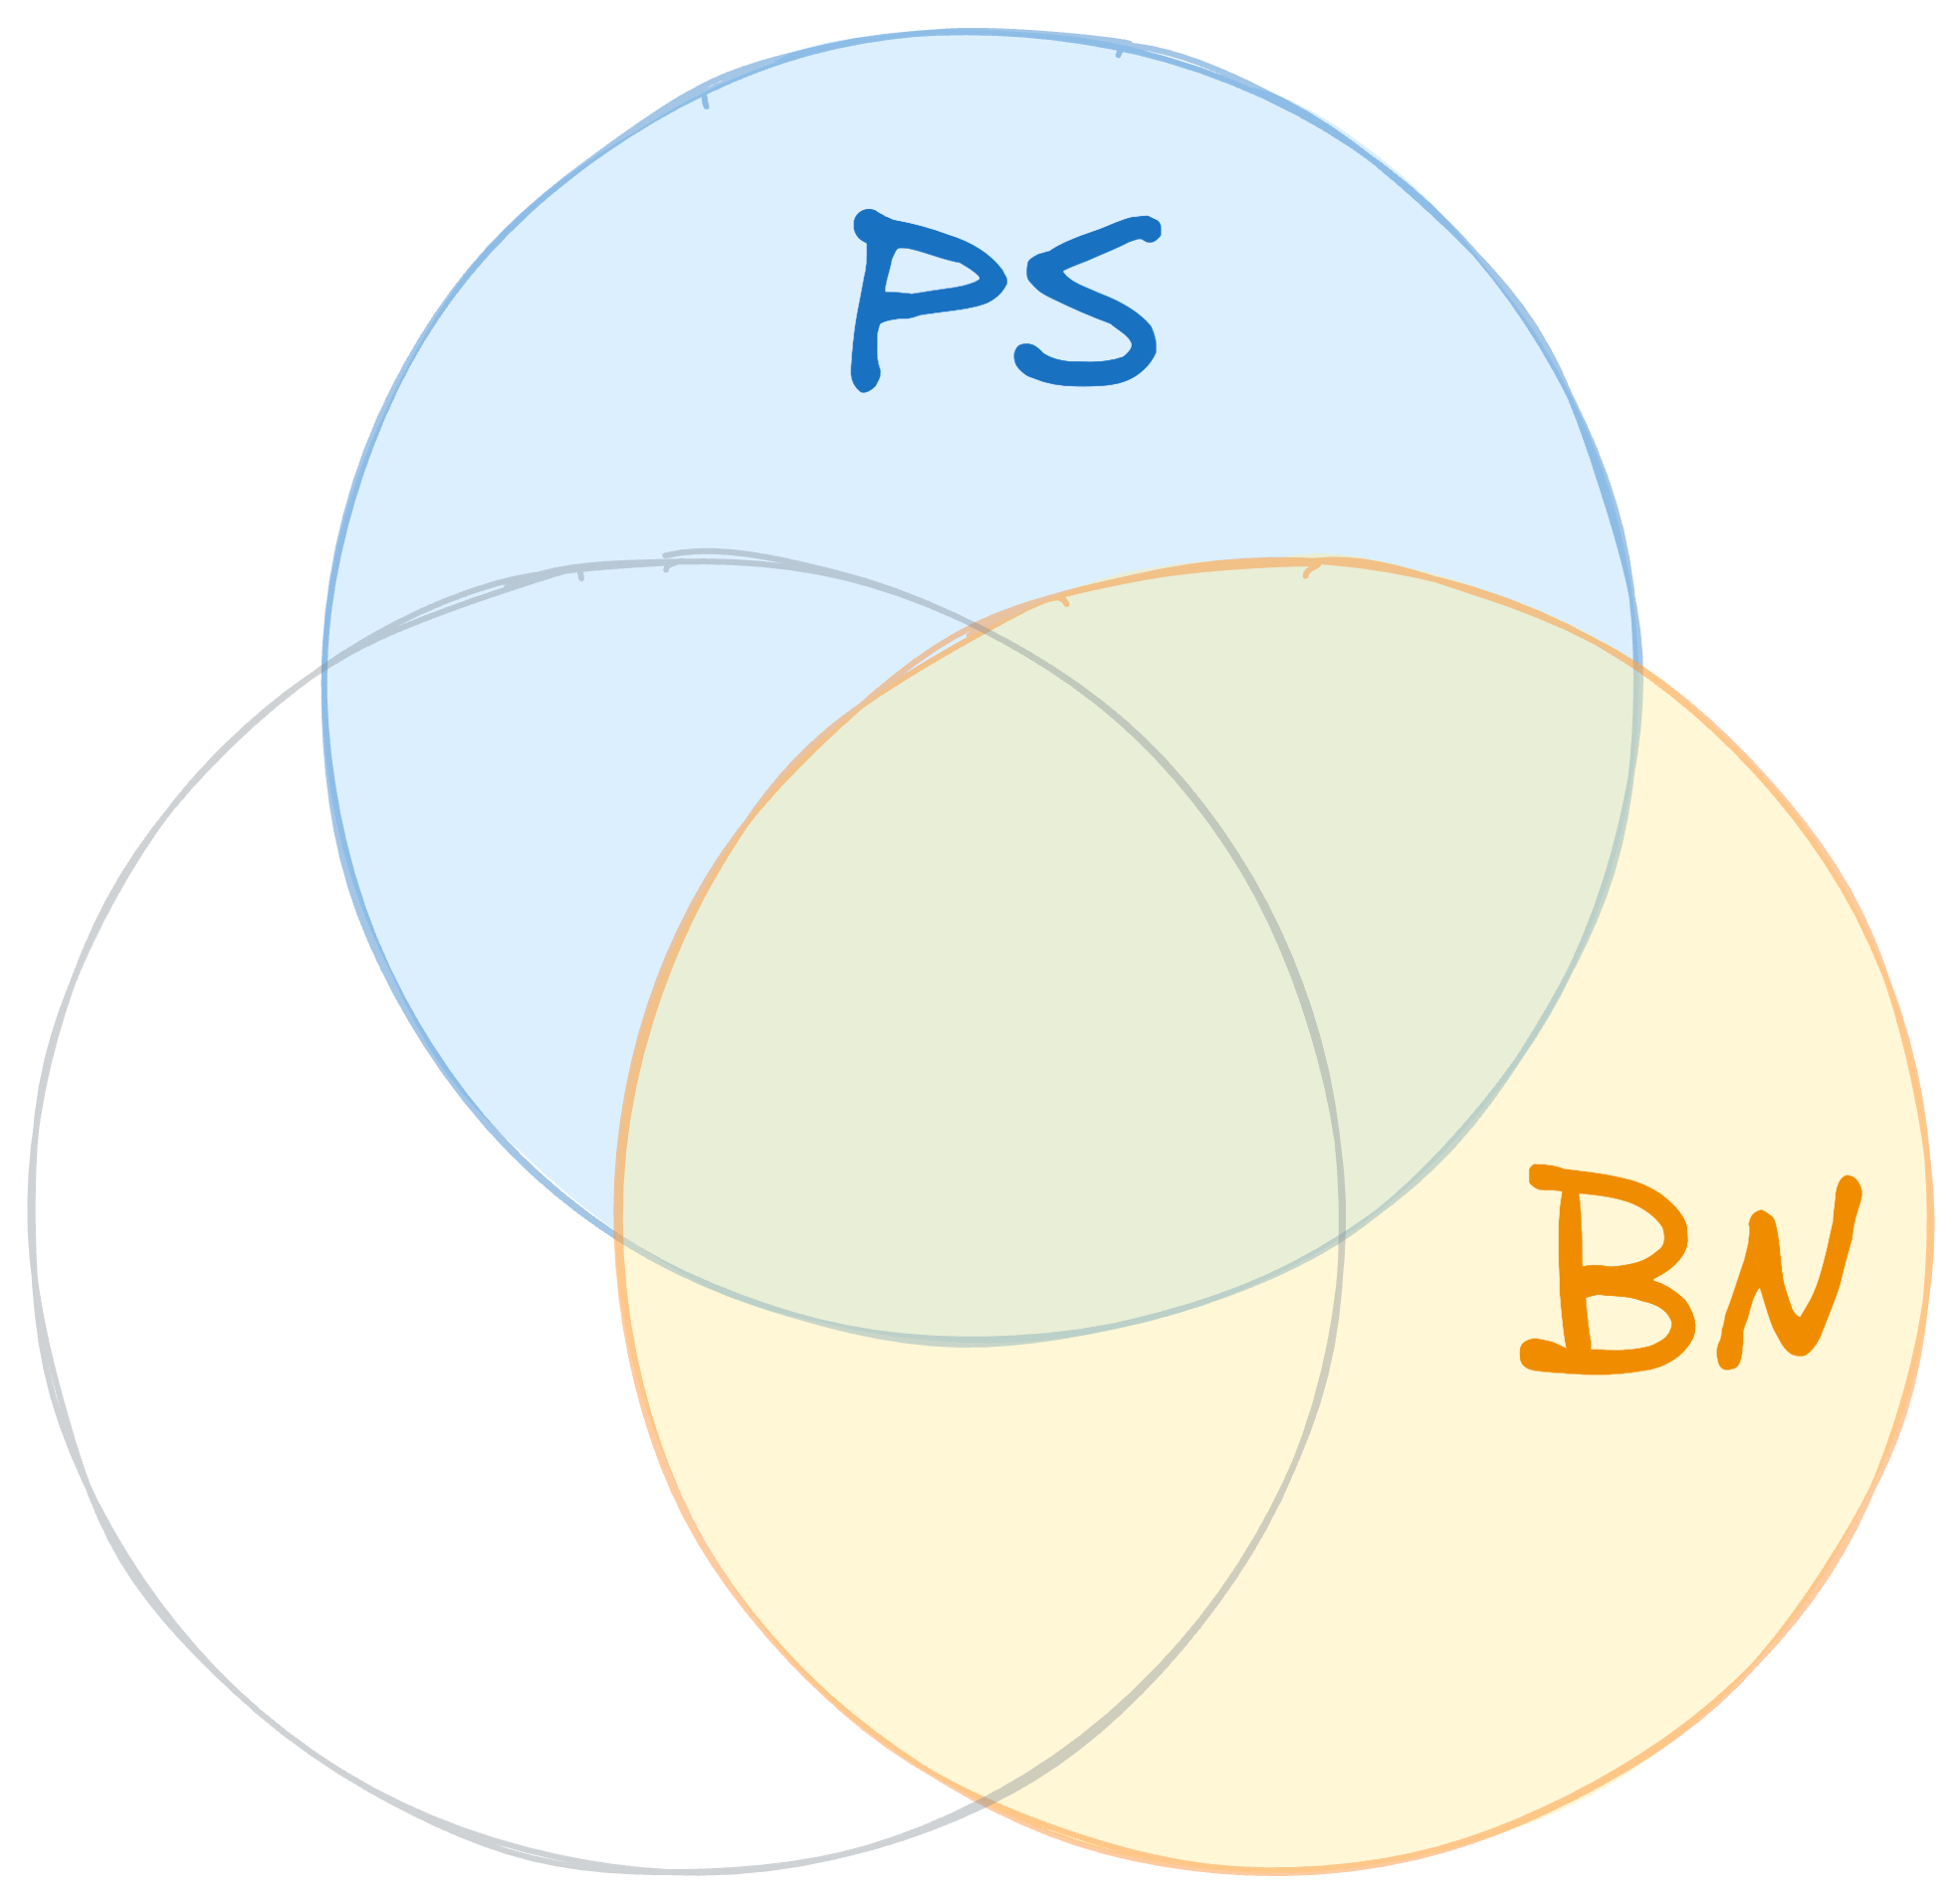
\includegraphics[width=\marginparwidth]{Figures/topics_ps_bns.png}
}


A shortcoming of classical Boolean networks as defined above is that to study network dynamics, all update functions must be fully specified. Moreover, the exact form of the update function might have little impact on observable behavior of the network (i.e., the attractor landscape).

Therefore, it was suggested to observe the dynamics of the Boolean network in context of of Boolean networks ensembles first~\cite{Kauffman2004,Schwab2020}. In this approach, we consider a set of Boolean networks that share some common properties (e.g., the same network structure or the same values of certain variables in their attractors). The goal is to study the dynamics of the whole ensemble instead of a single network. This way, we can obtain more robust results that are not dependent on a specific choice of update functions. 

The ensemble approach described as above, however, has its limitations, as it is not formalized very well and is usually limited to simulations. To address this problem, we consider the notion of \emph{Partially Specified Boolean Networks} (PSBNs)~\cite{Benes2019,benevs2022bdd} (sometimes also termed parametrized Boolean networks or colored Boolean networks). 

In a PSBN, we use \emph{function symbols} as stand-ins for unknown (fixed but arbitrary) parts of the network's unspecified dynamics. Therefore, the dynamics of a variable are either denoted by a standard (fully specified) function or by its function symbol and input arguments.
\begin{definition}
	Let $n$ be the number of variables, and $\allFunSymbols = \{\funSymbol_1,  \dots, \funSymbol_m \}$ a set of \emph{function symbols}. A \emph{partially specified Boolean network} $\pbnMath = \{ \expr_1, \ldots, \expr_n \}$ consists of function symbol expressions given by the following grammar:
	$$
		\expr ::= 0 \mid 1 \mid x \mid \neg \expr \mid \expr \land \expr \mid \expr \lor \expr \mid \funSymbol^{(a)}(\expr, \ldots, \expr) 
	$$
	Here, $x$ ranges over the network variables and $\funSymbol$ over the function symbols of $\allFunSymbols$ (superscript $a \in \mathbb{N}_0$ denotes the arity of $\funSymbol$). Other Boolean operators (e.g. $\Rightarrow$ or $\Leftrightarrow$) can be implemented as syntactic abbreviations using $\lor$, $\land$, and $\neg$.
\end{definition}

In other words, a PSBN is defined using standard Boolean constants ($0$ and $1$), variable state propositions ($x_i$) and Boolean connectives ($\neg$, $\land$, $\lor$), but it can also use function symbols from $\allFunSymbols$ as a way of expressing unknown behavior. This makes it possible to idiomatically describe systems whose dynamics are not fully known (see \autoref{example:psbn}).

\subsection{Interpretations and instances}

To give meaning to a particular $\pbnMath$, we rely on the term \emph{interpretation}. Formally, an interpretation $\interpretation$ is a set of $\{i_1, \ldots, i_m \}$ Boolean functions such that for each $\funSymbol^{(a)} \in \allFunSymbols$, there is a corresponding Boolean function $i^{(a)} \in \interpretation$ of the matching arity $a$. 

Intuitively, an interpretation associates a specific Boolean function to every function symbol. Consequently, we can substitute all symbols $\funSymbol \in \allFunSymbols$ for functions $i \in \interpretation$ in a $\allFunSymbols = \{\funSymbol_1, \ldots, \funSymbol_n\}$ of a $\pbnMath$, and a result we obtain a collection of $n$ fully specified functions. The result is a \emph{Boolean network instance} which we denote as $\pbnMath(\interpretation)$ and which has the same semantics as a standard BN. The set of all possible interpretations of $\allFunSymbols$ is denoted as $\allInterpretations(\allFunSymbols)$ or $\allInterpretations$ for short (i.e., when the context is clear). Some subset of interpretations is then referred to as $\interpretationSet \subseteq \allInterpretations$. 

\subsection[Normalization of PSBN]{Normalization of partially specified Boolean networks}

Function symbols are practical as a human-friendly specification language of unknown network behavior. However, it is not entirely clear how algorithms should represent such functions symbolically, as is our goal in this paper. To alleviate this issue, we note the following: Assuming that all $m$ function symbols in $\allFunSymbols$ have arity zero, possible interpretations $\allInterpretations$ of $\allFunSymbols$ correspond to the vectors $\bools^{m}$. This is because a nullary function symbol is necessarily a constant and can be thus interpreted as a Boolean value. We call such zero arity symbols \emph{zero-arity symbols} (we can also simply write $\funSymbol$ instead of $\allFunSymbols^{(0)}()$ when using such symbols). In some literature, these are also referred to as network inputs~\cite{Kobayashi2011}. 

Given any $\pbnMath$, we can produce a \emph{normalized} $\widehat{\pbnMath}$ that only uses a fresh set of logical nullary function symbols $\widehat{\allFunSymbols}$ instead of general function symbols $\allFunSymbols$, but its interpretations are the same fully specified BNs as for the original $\pbnMath$. To implement this normalization, we use the following expansion rule (here, $\expr_1, \ldots, \expr_a$ are arbitrary Boolean expressions):
\begin{align*}
	\allFunSymbols^{(a)}(\expr_1, \ldots, \expr_a) &\equiv (\expr_1 \Rightarrow \mathcal{F}^{(a-1)}_P(\expr_2, \ldots, \expr_a)) \\
    &\land (\neg \expr_1 \Rightarrow \funSymbol^{(a-1)}_N(\expr_2, \ldots, \expr_a))
\end{align*}

This rule transforms any expression using a function symbol $\funSymbol$ of arity $a$ into an expression using two fresh function symbols of arity $a-1$ ($\funSymbol_P$ and $\funSymbol_N$). Interpretations of the original and the transformed expression result in the same concrete Boolean functions. By recursively applying this rule, we can transform any $\funSymbol^{(a)}$ into $2^a$ nullary function symbols, each corresponding to one row of the truth table of the original $\funSymbol$. Without the loss of generality, we can thus assume that the interpretations of a particular $\pbnMath$ are identified by the members of $\bools^{m}$ for some $m = |\widehat{\allFunSymbols}|$. The set of all interpretations is then exactly equivalent to  $\allInterpretations = \bools^m$. An example of a normalized $\widehat{\pbnMath}$ is given in \autoref{example:psbn}.

We must not forget, that the basis of BNs (and PSBNs) are the regulatory networks as described in \autoref{s:reg_net}. Therefore, if we have a definition of an expression for $x_1$ given as $\expr_1 \equiv \funSymbol(x_1, x_2)$, and we know, that $x_2$ has a down-regulating effect on $x_1$, the functional symbol $\funSymbol$ should \textbf{not} be replaced by a function $x_1 \lor x_2$.

To address this, we will consider the set $\allInterpretations$ to contain only \emph{consistent} interpretations*.\marginpar{*More on the topic of consistent interpretations can be found in a line of work on Boolean networks refinement \cite{Benes2023}.}
 An interpretation $\interpretation$ is consistent with a given regulatory network if for every variable $x_i$ and its corresponding expression $\expr_i$, the function $f_i$ obtained by substituting all function symbols in $\expr_i$ with their corresponding functions from $\interpretation$ respects the regulatory structure of the network. The restrictions on regulations can be found in \autoref{ss:bn_definition}. 

\subsection{Colored state transition graph}
\label{ss:psbn_stg}

\marginpar{*Note, that update schema of PSBNs is different from the probabilistic BNs mentioned in \autoref{ss:updating_schemes}. In particular, the probabilistic semantics use multiple update functions for the same variable within a single run while PSBN considers only a single instance (interpretation) for each run.}
With this knowledge in mind, we can define a \emph{colored} state-transition graph that collectively encodes the behavior of all possible interpretations of a particular $\pbnMath$ using only Boolean values*. In this representation, the interpretations of the normalized $\widehat{\pbnMath}$ (the members of $\bools^m$) each define a potentially different transition relation over the shared state space $\bools^n$:

\begin{definition}
	Let $\widehat{\pbnMath} = \{ \expr_1, \ldots, \expr_n \}$ be a normalized partially specified Boolean network such that $\widehat{\pbnMath}$ admits $m$ nullary function symbols $\allFunSymbols = \{\funSymbol_1, \ldots, \funSymbol_m \}$. The \emph{labelled state-transition graph} $\STG(\widehat{\pbnMath}) = (\vertices, \allInterpretations, \edges)$ is a directed graph where $\vertices = \bools^n$, $\allInterpretations = \bools^m$ and $\edges \subseteq \vertices \times \allInterpretations \times \vertices$ is given as $(u, \interpretation, v) \in \edges \Leftrightarrow (u,v) \in \edges(\STG(\widehat{\pbnMath}(\interpretation)))$. We write a state transition under $\interpretation$ as $u \to_{\interpretation} v$. The set of all interpretations enabling a transition from $u$ to $v$ is denoted as $\interpretationSet(u,v) = \{\interpretation \mid (u, \interpretation, v) \in \edges\}$.
\end{definition}

In other words, the labelled state-transition graph is a unifying structure that incorporates the STG of all instances of $\pbnMath$: A transition from a state $u$ to state $v$ is enabled for an interpretation $\interpretation$ if the same transition appears in the STG of $\pbnMath(\interpretation)$. Similarly, we consider \PBN{} runs in the context of a specific interpretation $\interpretation$ (or instance) denoted as $\allRuns_\interpretation$. An example of an STG of a \PBN{} instance is depicted in \autoref{fig:psbn}. We further explore the usefulness of labelled STGs in \textcolor{red}{Section REF}, where we show how these can be efficiently manipulated symbolically.

\begin{example}
	\label{example:psbn}
	Consider a PSBN $\pbnMath$ with $\allFunSymbols = \{ \funSymbol^{(2)}\}$ and given by three expressions: 
    \begin{align*}
    \expr_1 &\equiv \funSymbol(x_1, x_2) \\
    \expr_2 &\equiv x_1 \land x_3 \\
    \expr_3 &\equiv x_1 \lor \neg x_3
    \end{align*}
    After normalization, we have $\widehat{\allFunSymbols} = \{ \funSymbol_{00}, \funSymbol_{01}, \funSymbol_{10}, \funSymbol_{11} \}$ and expressions:
    \begin{align*}
        \widehat{\expr}_1 &\equiv ((\neg x_1 \land \neg x_2) \Rightarrow \funSymbol_{00}) \\
        &\land ((\neg x_1 \land x_2) \Rightarrow \funSymbol_{01}) \\
        &\land ((x_1 \land \neg x_2) \Rightarrow \funSymbol_{10}) \\
        &\land ((x_1 \land x_2) \Rightarrow \funSymbol_{11}) \\
        \widehat{\expr}_2 &\equiv x_1 \land x_3 \\
        \widehat{\expr}_3 &\equiv x_1 \lor \neg x_3
    \end{align*}
\end{example}


\begin{figure}[htp]
    \centering
    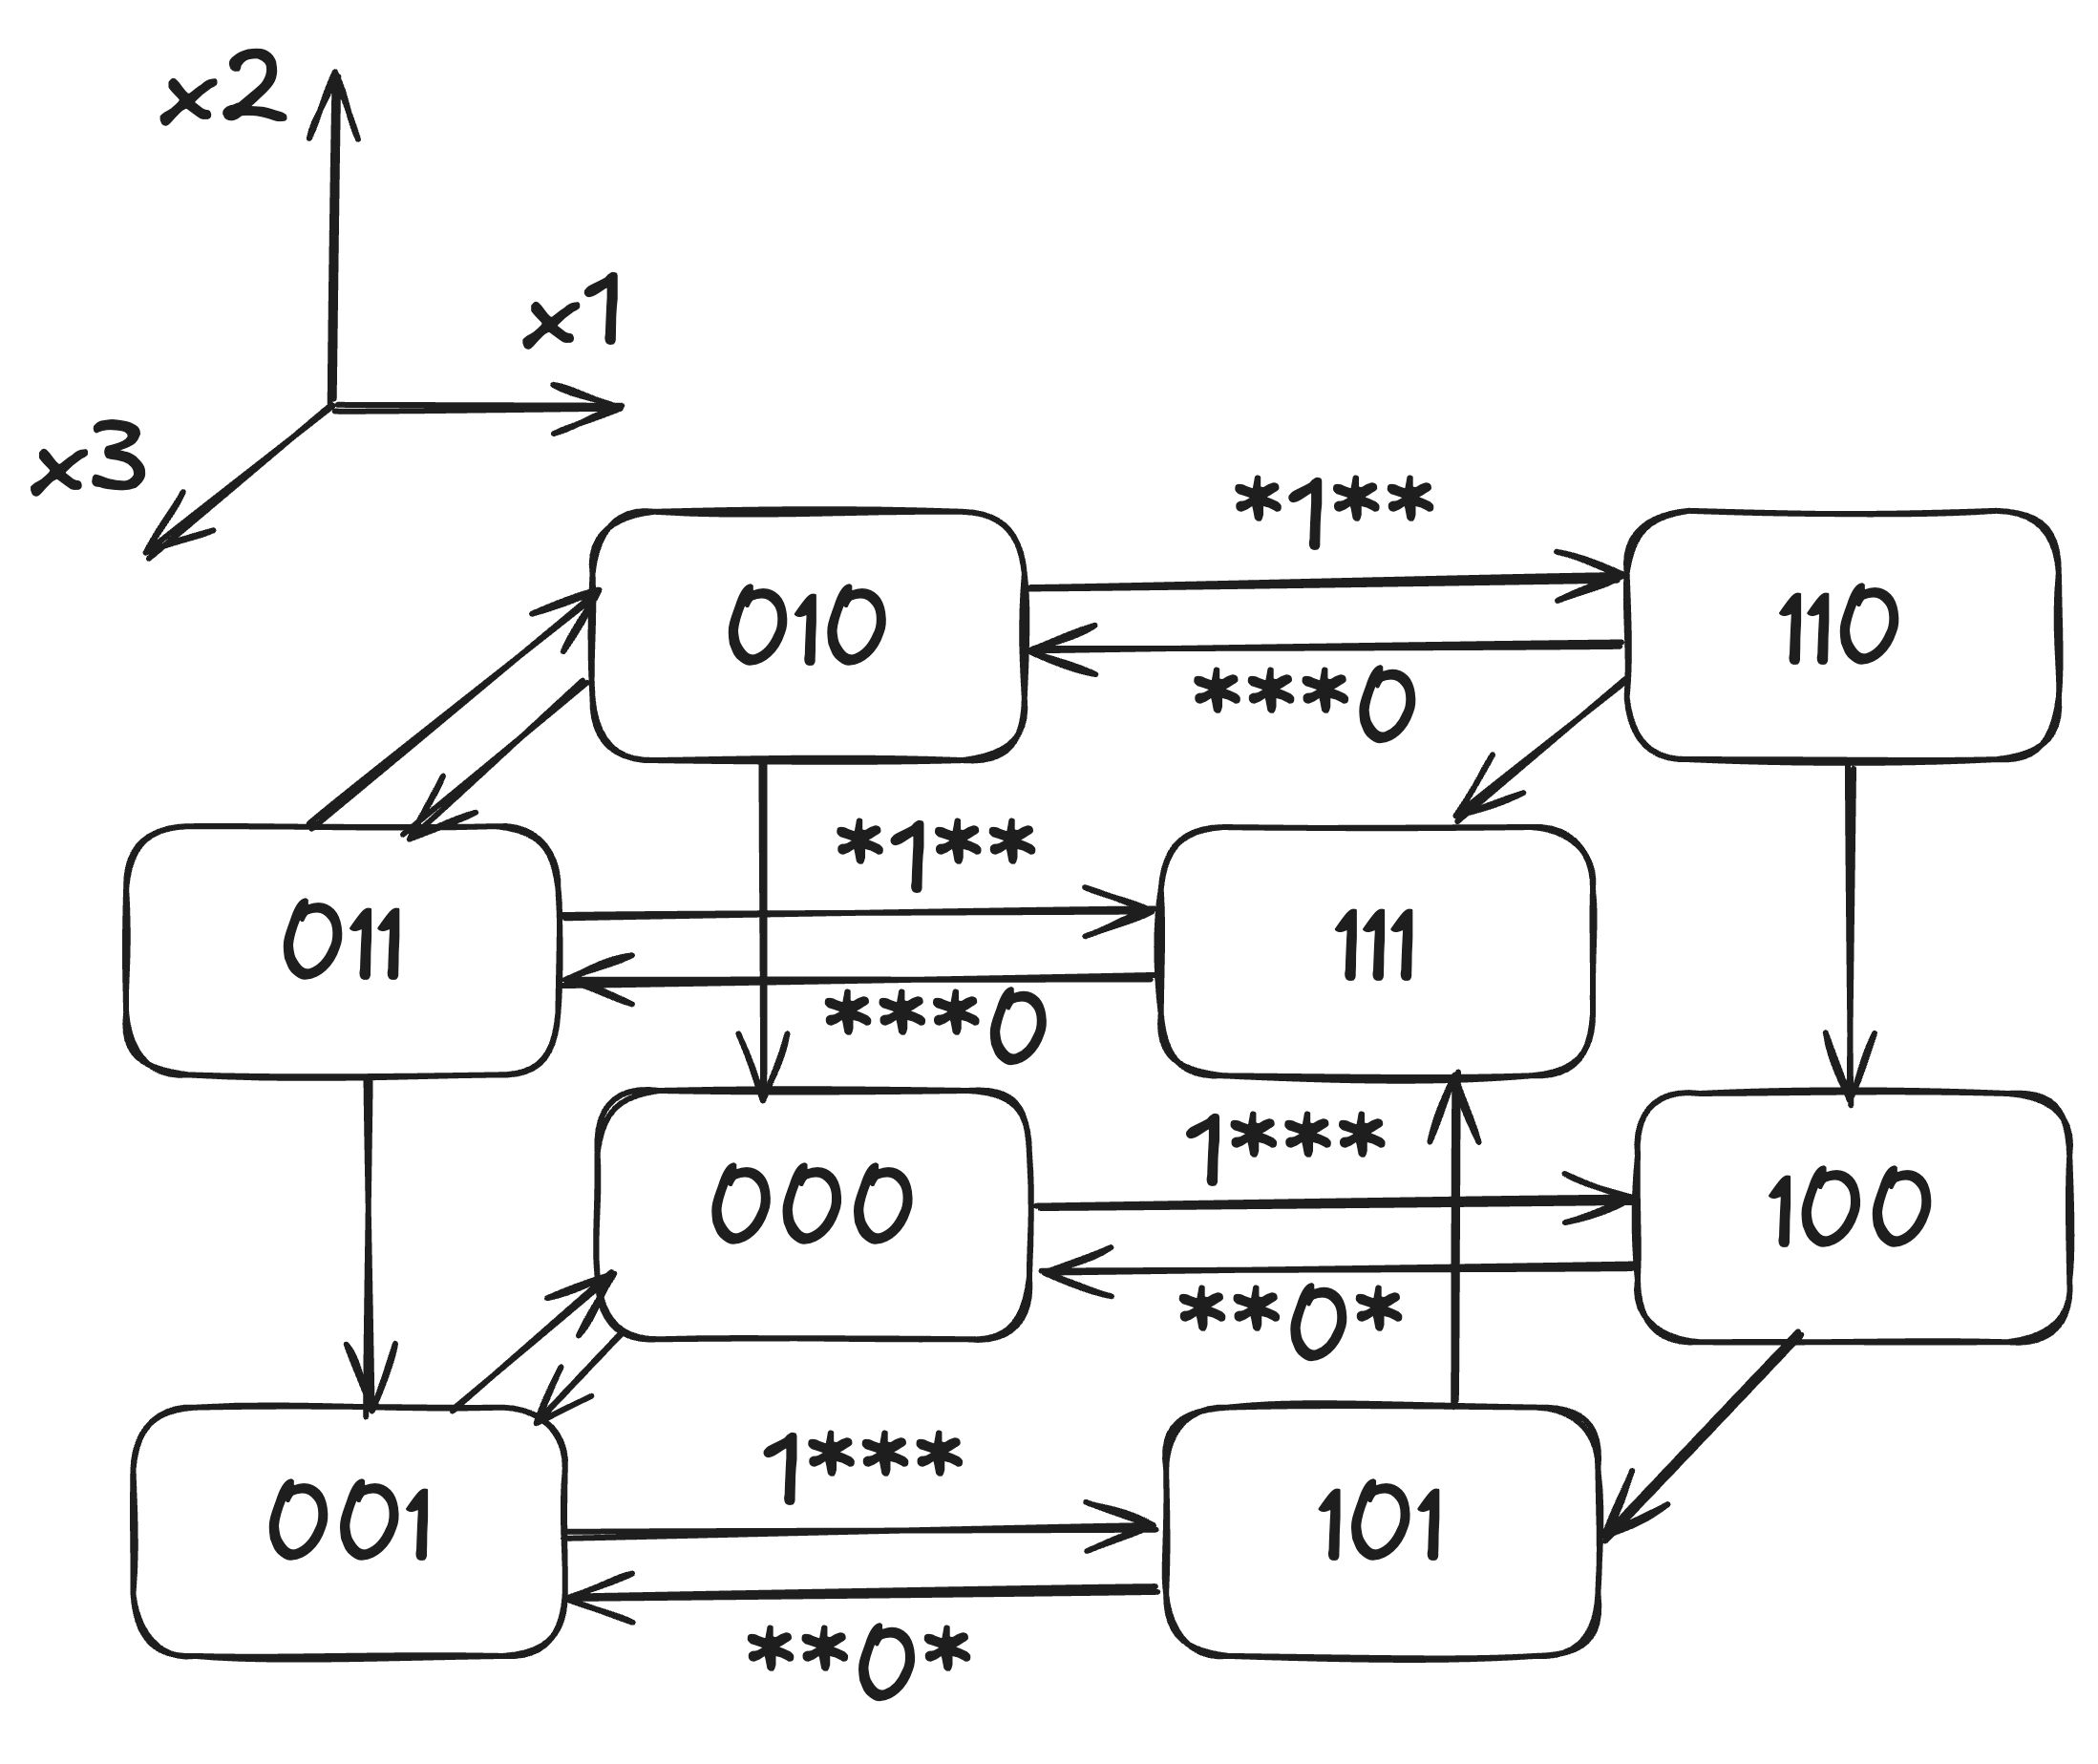
\includegraphics[width=0.5\textwidth]{Figures/psbn_state_space.png}
    \caption{\textbf{State-transition graph of a PSBN.} Figure shows the state-transition graph of a PSBN from \autoref{example:psbn}. The labels of edges represent all interpretations for which the edge is admissible. For brevity, edges admissible in all instances are drawn without a label while edges admissible for no instance are not depicted in the figure at all.}
    \label{fig:psbn}
\end{figure}


Given the notions of labelled STG and a PSBN instance, we can transfer the state space structures previously introduced for BNs to the PSBN setting. We will not focus on the control and perturbation notions, since they are part of the contribution of the thesis and are described in \autoref{chapter:source_target_control} and \autoref{chapter:phenotype_control_psbn}.

The notions which are independent transitions such as character, trait and phenotype do not depend on the actual dynamics of the network (only on its variables) are identical for BNs and PSBNs.

Definitions of trap set, attractor, attractor's weak and strong basins for fully specified BNs are lifted to PSBNs per individual instances (interpretations). For example, we write that a set $\attractor \subseteq \vertices$ is an attractor for an instance $\pbnMath(\interpretation)$ (i.e. there are no attractors of $\pbnMath$, only attractors of its instance). 

\subsection[Well-known problems on PSBNs]{Well-known problems on partially specified Boolean networks}

Now that we have defined PSBNs, we can also consider well-known problems solved for this type of models, in order to understand the challenges they present and give us a better understanding of the tools we can use to solve the control problems. Or vice versa, we can also consider how the control problems can be used to solve the well-known problems on PSBNs.

\subsubsection{Attractor search}

Attractor search in PSBNs involves identifying sets of states (attractors) that the system tends to evolve towards, regardless of the initial state. This is crucial for understanding the long-term behavior of the networks. As opposed to fully specified BNs, PSBNs can have a significantly larger number of attractors due to the uncertainty in their dynamics. Moreover, the attractors can differ across instances, leading to a more complex attractor landscape.

For PSBNs, usually the approaches from fully specified BNs are applied, but they are either highly parallelized or adjusted to work with the labelled STG. For example, one can use symbolic methods to represent and manipulate the state space efficiently, allowing for the exploration of multiple interpretations simultaneously~\cite{benevs2022bdd,Pauleve2023b}.

In context of control, attractor search is often a preliminary step to identify potential target states or behaviors that we want to achieve through control interventions. It also serves as a good last step to verify if the control objectives have been met.

\subsubsection{Bifurcation}

As described before, bifurcation analysis studies how changes in parameters (in the case of PSBNs, interpretations) can lead to qualitative changes in the system's dynamics. In PSBNs, this involves examining how different interpretations affect the attractor landscape and identifying critical interpretations that lead to significant changes in behavior~\cite{Benes2022, Pastva2022}.

This problem is particularly relevant in biological contexts, where certain gene regulatory networks may exhibit different behaviors under varying conditions or mutations. Bifurcation analysis can help identify these critical points and understand the robustness of the network's behavior.

In context of control of PSBNs, bifurcation analysis again can be used as an aid for attractor search and deciding suitable target attractors. 

\subsubsection{Model checking}

Model checking in PSBNs involves verifying whether certain properties or specifications hold across all possible interpretations of the network. This is particularly challenging due to the combinatorial explosion of possible interpretations, but it is essential for ensuring that the network behaves as expected under various conditions~\cite{Benes2023}. 

Model checking can be used to verify safety properties (e.g., certain undesirable states are never reached), liveness properties (e.g., certain desirable states are eventually reached), and other temporal properties of interest. In the context of control, model checking can be used to verify whether the control strategies employed lead to the desired outcomes across all interpretations of the PSBN.

\subsubsection{Model refinement}

All the methods above are also often used for the grand objective of \emph{model refinement}, which aims to reduce the uncertainty in a PSBN by eliminating interpretations that are inconsistent with observed data or desired properties. This process helps in narrowing down the set of possible network behaviors, making the model more precise and reliable~\cite{Benes2023}. Such a model is more likely to yield accurate predictions and insights into the underlying biological processes.

In the context of control, model refinement can help in identifying more effective control strategies by omitting spurious network behaviors. But also vice versa, as we describe in \autoref{chapter:applications}, we suggest control to be used as another tool for model refinement.

\section{Summary}

In this chapter, we have introduced the necessary background for understanding the control of Boolean networks. We started by defining regulatory networks, and Boolean networks and their dynamics, including the concept of attractors and basins of attraction.

We then discussed various control objectives, types of perturbations that can be applied to control the network, including one-step, temporary, and permanent perturbations, as well as their temporal properties.

Finally, we introduced partially specified Boolean networks, which allow for the representation of uncertainty in network dynamics, and discussed their normalization and the concept of a colored state transition graph. 

This foundational knowledge sets the stage for the subsequent chapters, where we will delve into specific control strategies and algorithms for both fully specified (in terms of state of the art) and partially specified Boolean networks (in terms of contribution of this thesis).

\chapter{State of the Art}
\label{chap:sota}
% Motivation and definition

In this chapter, we will discuss the state of the art related to control of Boolean networks. We will start with a brief overview of the history of control theory and control of partially specified systems. We will then focus on control of synchronous, asynchronous and most-permissive BN which served as an inspiration of development of the \PBN{} control methods presented in the following chapters (\autoref{chapter:source_target_control} and \autoref{chapter:phenotype_control_psbn}). Next, we discuss overlap and applicability of control to the problematic of model inference. Finally, we exhaustively compare the existing control methods and tools in the field of BN control and discuss the limitations of the existing methods and tools.

\section{Control of discrete systems}
\marginpar{
    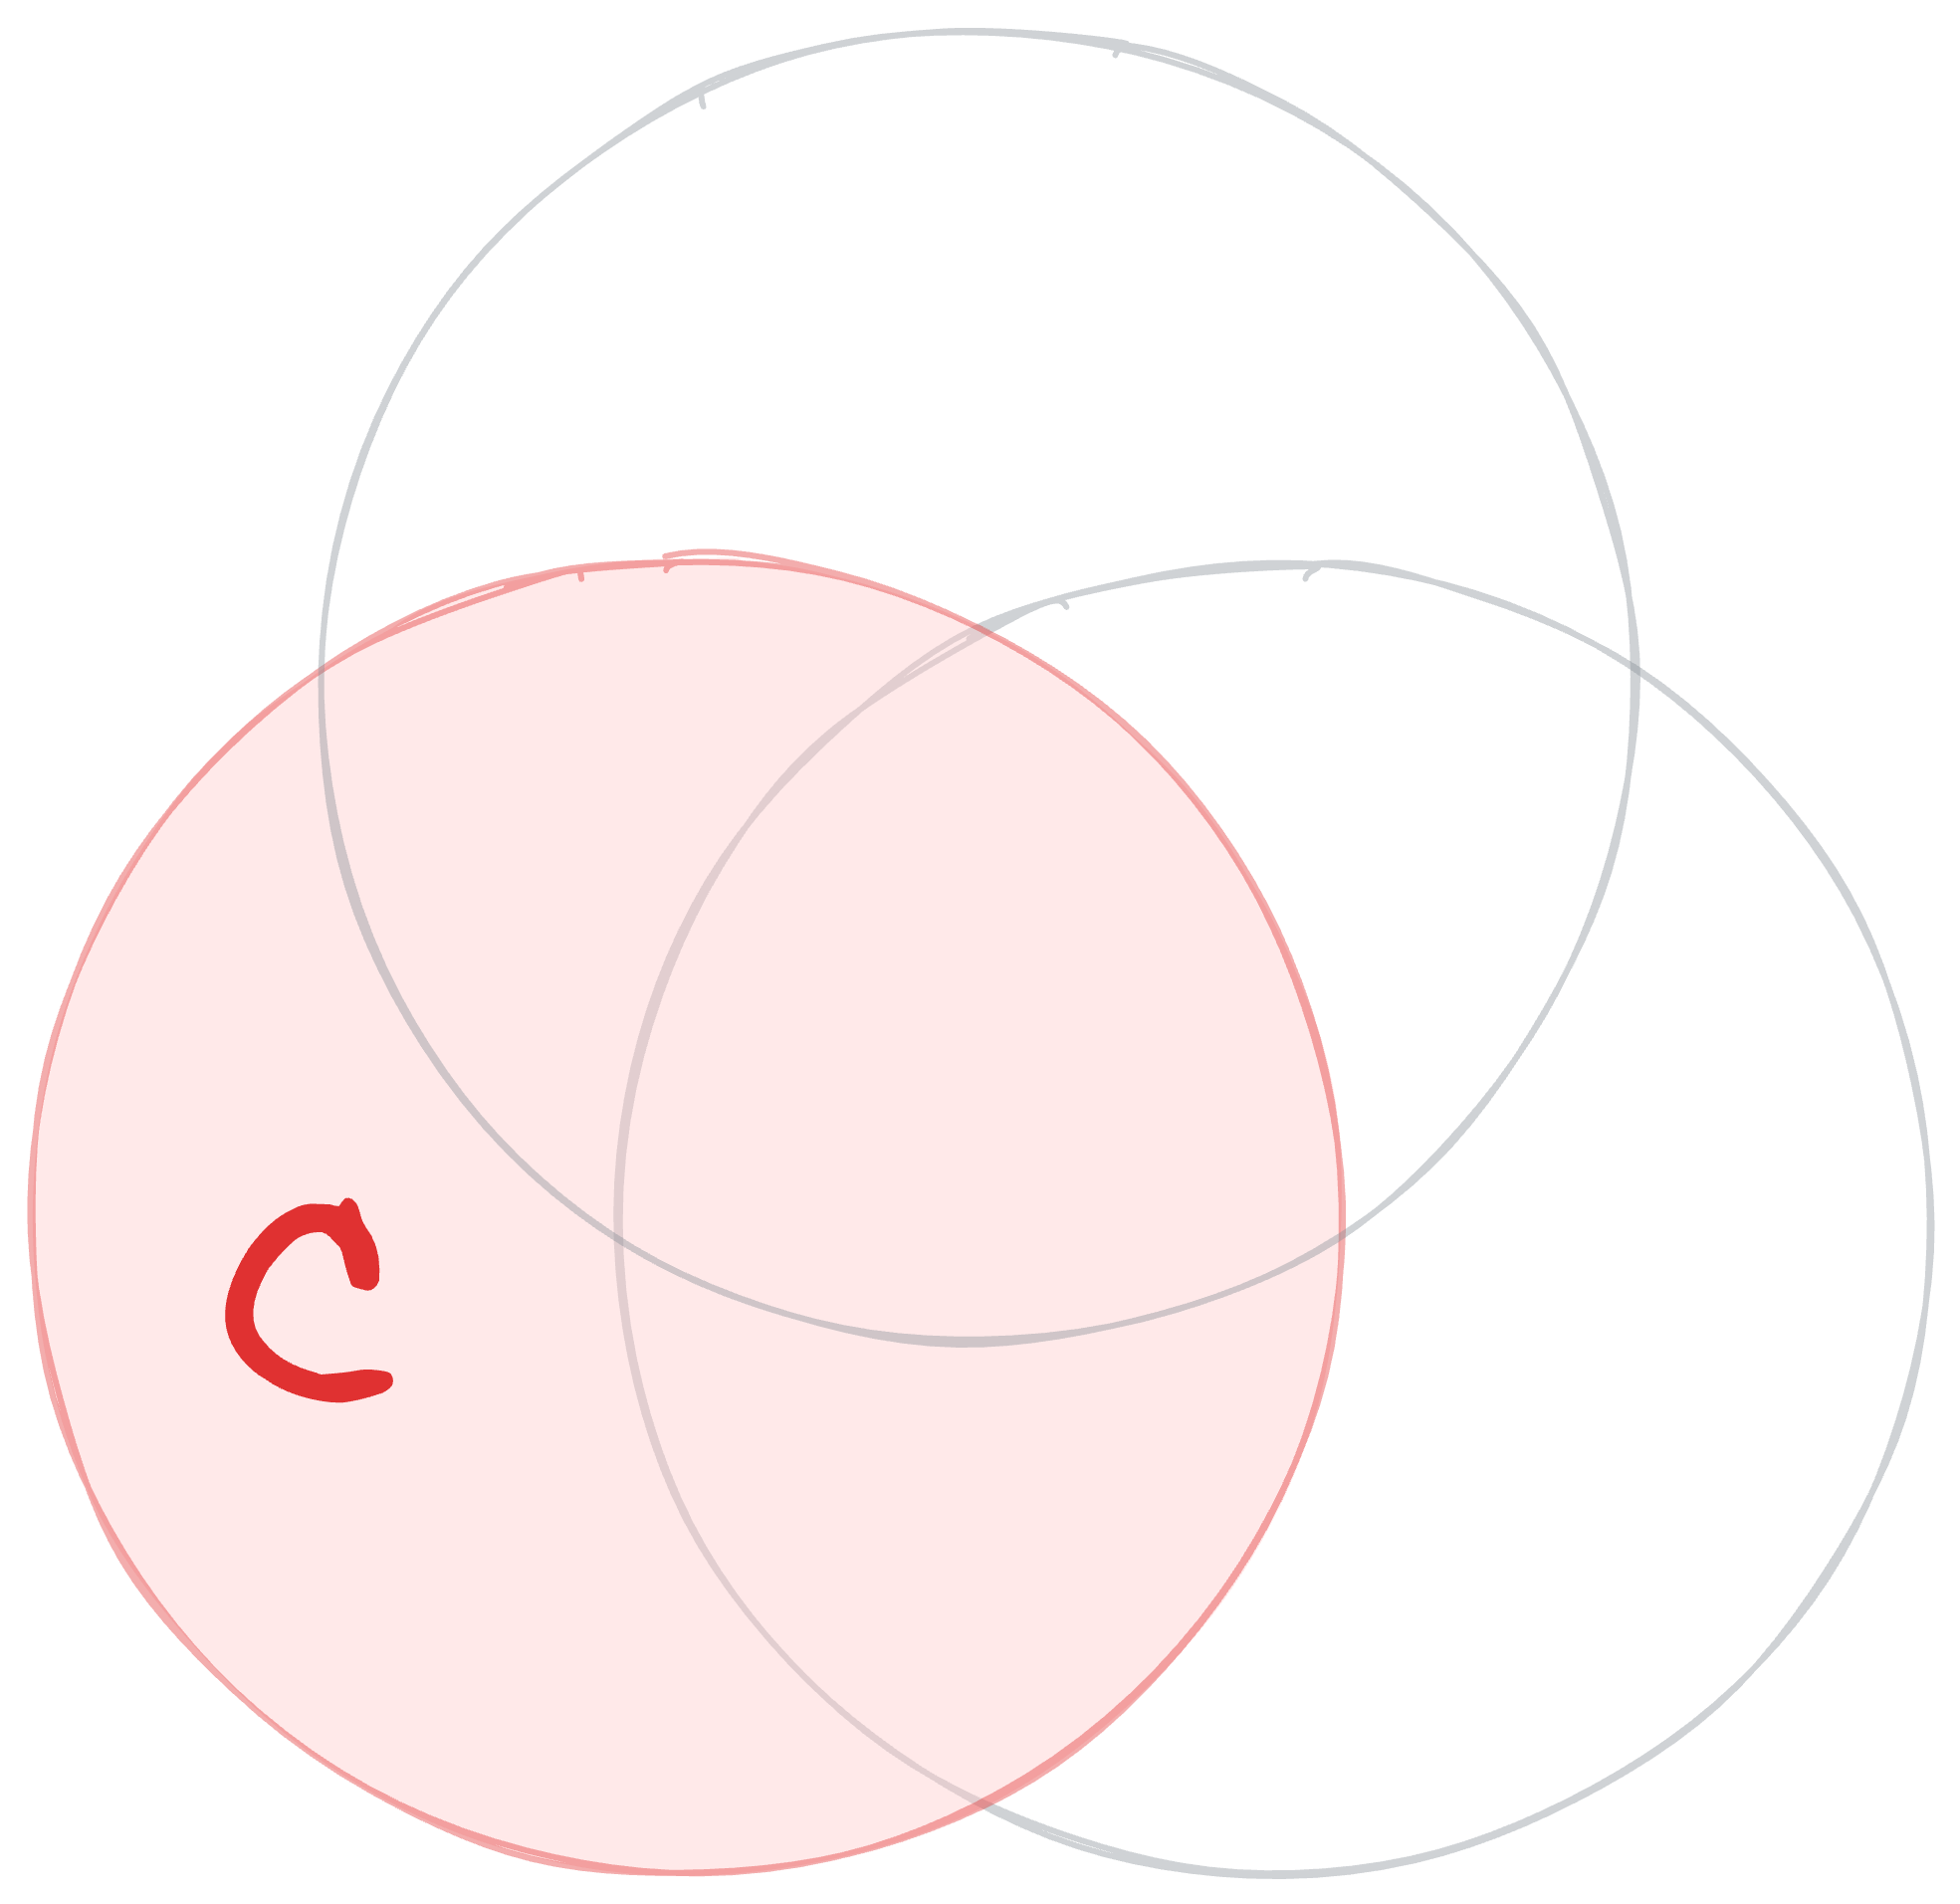
\includegraphics[width=\marginparwidth]{Figures/topics_ctrl.png}
}
\label{sec:controlDiscrete}

% History since Maxwell & slightly before
The field of control theory has an extensive historical background, tracing back to the 19th century when James Clerk Maxwell formalized the principles of feedback through his seminal work on governors~\cite{Maxwell1868}. These mechanical regulators, such as the centrifugal governor used to maintain windmill speed~\cite{Fernandez2003}, embodied some of the earliest notions of automatic control, though their application was predominantly focused on systems governed by continuous dynamics.

% First Discrete systems control -> relay circuits
As engineering advanced into the early 20th century, a paradigm shift towards discrete systems began with the rise of relay logic and switching circuits. Pioneered by Claude Shannon in his groundbreaking master's thesis~\cite{Shannon1938,Shannon1940}, the application of Boolean algebra to electrical circuits laid the foundation for the control of discrete systems. This marked the transition from purely continuous control to symbolic, state-based reasoning in control design.


% Cybernetics overarching
The 1940s brought a unifying conceptual breakthrough with the emergence of cybernetics. Led by Norbert Wiener, who was himself inspired by Maxwell’s early insights, cybernetics established a theoretical framework for feedback, communication, and control across mechanical, biological and combined systems~\cite{Wiener1948}. This new perspective helped shape the modern view of control as a universal system principle,  leading to its widespread application in fields such as engineering, economics, cognitive science, and biology.

% DES
From this foundation, the control of discrete systems evolved into more specialized subfields. One of the most prominent is the control of discrete event systems (DES), introduced by Ramadge and Wonham~\cite{Ramadge1987}. In DES, the processes under control are modeled as asynchronous, discrete, and potentially nondeterministic systems. These systems are often described by formal languages, where the plant is represented as a language generator and the controller (or supervisor) as a recognizer of a target language. The central problem becomes the synthesis of the largest controllable sub-language that satisfies the desired specifications

% Model checking? Thin ice :/ 
One of the major advancement in the discrete systems theory is the development of model checking~\cite{Clarke1981,Clarke1997}. Model checking is a formal verification method used to determine whether a system model (e.g. a Kripke structure~\cite{Kripke1959,Kripke1963}) satisfies a temporal logic specification (e.g. a LTL~\cite{Pnueli1977}). It has been instrumental in verifying properties such as safety, liveness, and reachability. A \emph{parametric} model checking or ~\emph{parameter synthesis} then seeks to find the maximal set of parameters for which the property holds~\cite{Hune2002,Daws2004,Smijakova2020}.

% Model checking -> less (parameter) options, more general properties
% Control -> very specific property types, more flexible parameters/perturbations/interventions
Formulas such as ensuring a system "eventually reaches a desired state" can be also viewed as a direct reduction of the control problem. This brings us to a provocative question -- what is the relationship between control and parametric model checking? The two problems share a common goal of refining system behavior to meet certain specifications, but they approach the problem from different angles. Model checking typically operates within a well-defined domain of parameters and verifies whether a selected property (drawn from a wide variety of types) holds for a given system. 

Control theory, on the other hand, tends to focus on a narrower set of property types (i.e., reachability) but allows for greater flexibility in choosing parameters, applying perturbations, or designing other interventions to guide system behavior. Specifically, parameter synthesis typically infers a static system properties, whereas control might also apply temporal interventions. Therefore, narrowing the focus to a specific property type enables more efficient optimization for the problem at hand.

% Booelan control networks
The control of discrete systems eventually extended to the realm of BN theory thoroughly introduced in the previous chapter. Initially, Boolean \emph{control} networks (BCN) were considered as an object of the control~\cite{Akutsu2007,Cheng2010,Hochma2013,Zhao2015,Moradi2019}. BCNs are characteristic by containing a set of control (input) nodes and a set of controlled (output) nodes. The control problem lies in the assigning Boolean values to the given control inputs. This problem was extensively studied and successfully solved e.g. using algebraic and semi-tensor product methods~\cite{Cheng2010} or model checking~\cite{Langmead2009}. 

It could be argued, that BCN control problem is more similar to the flavor of parameter synthesis, than to the control of discrete event systems, since the control inputs are given whereas the control we focus on in this thesis is having more flexibility in the selected perturbations. Nonetheless, as we will see later, in our approach BN inputs are also utilized to control the system, nonetheless in a far more tailored way.

\section{Control of partially specified systems} 
\marginpar{
    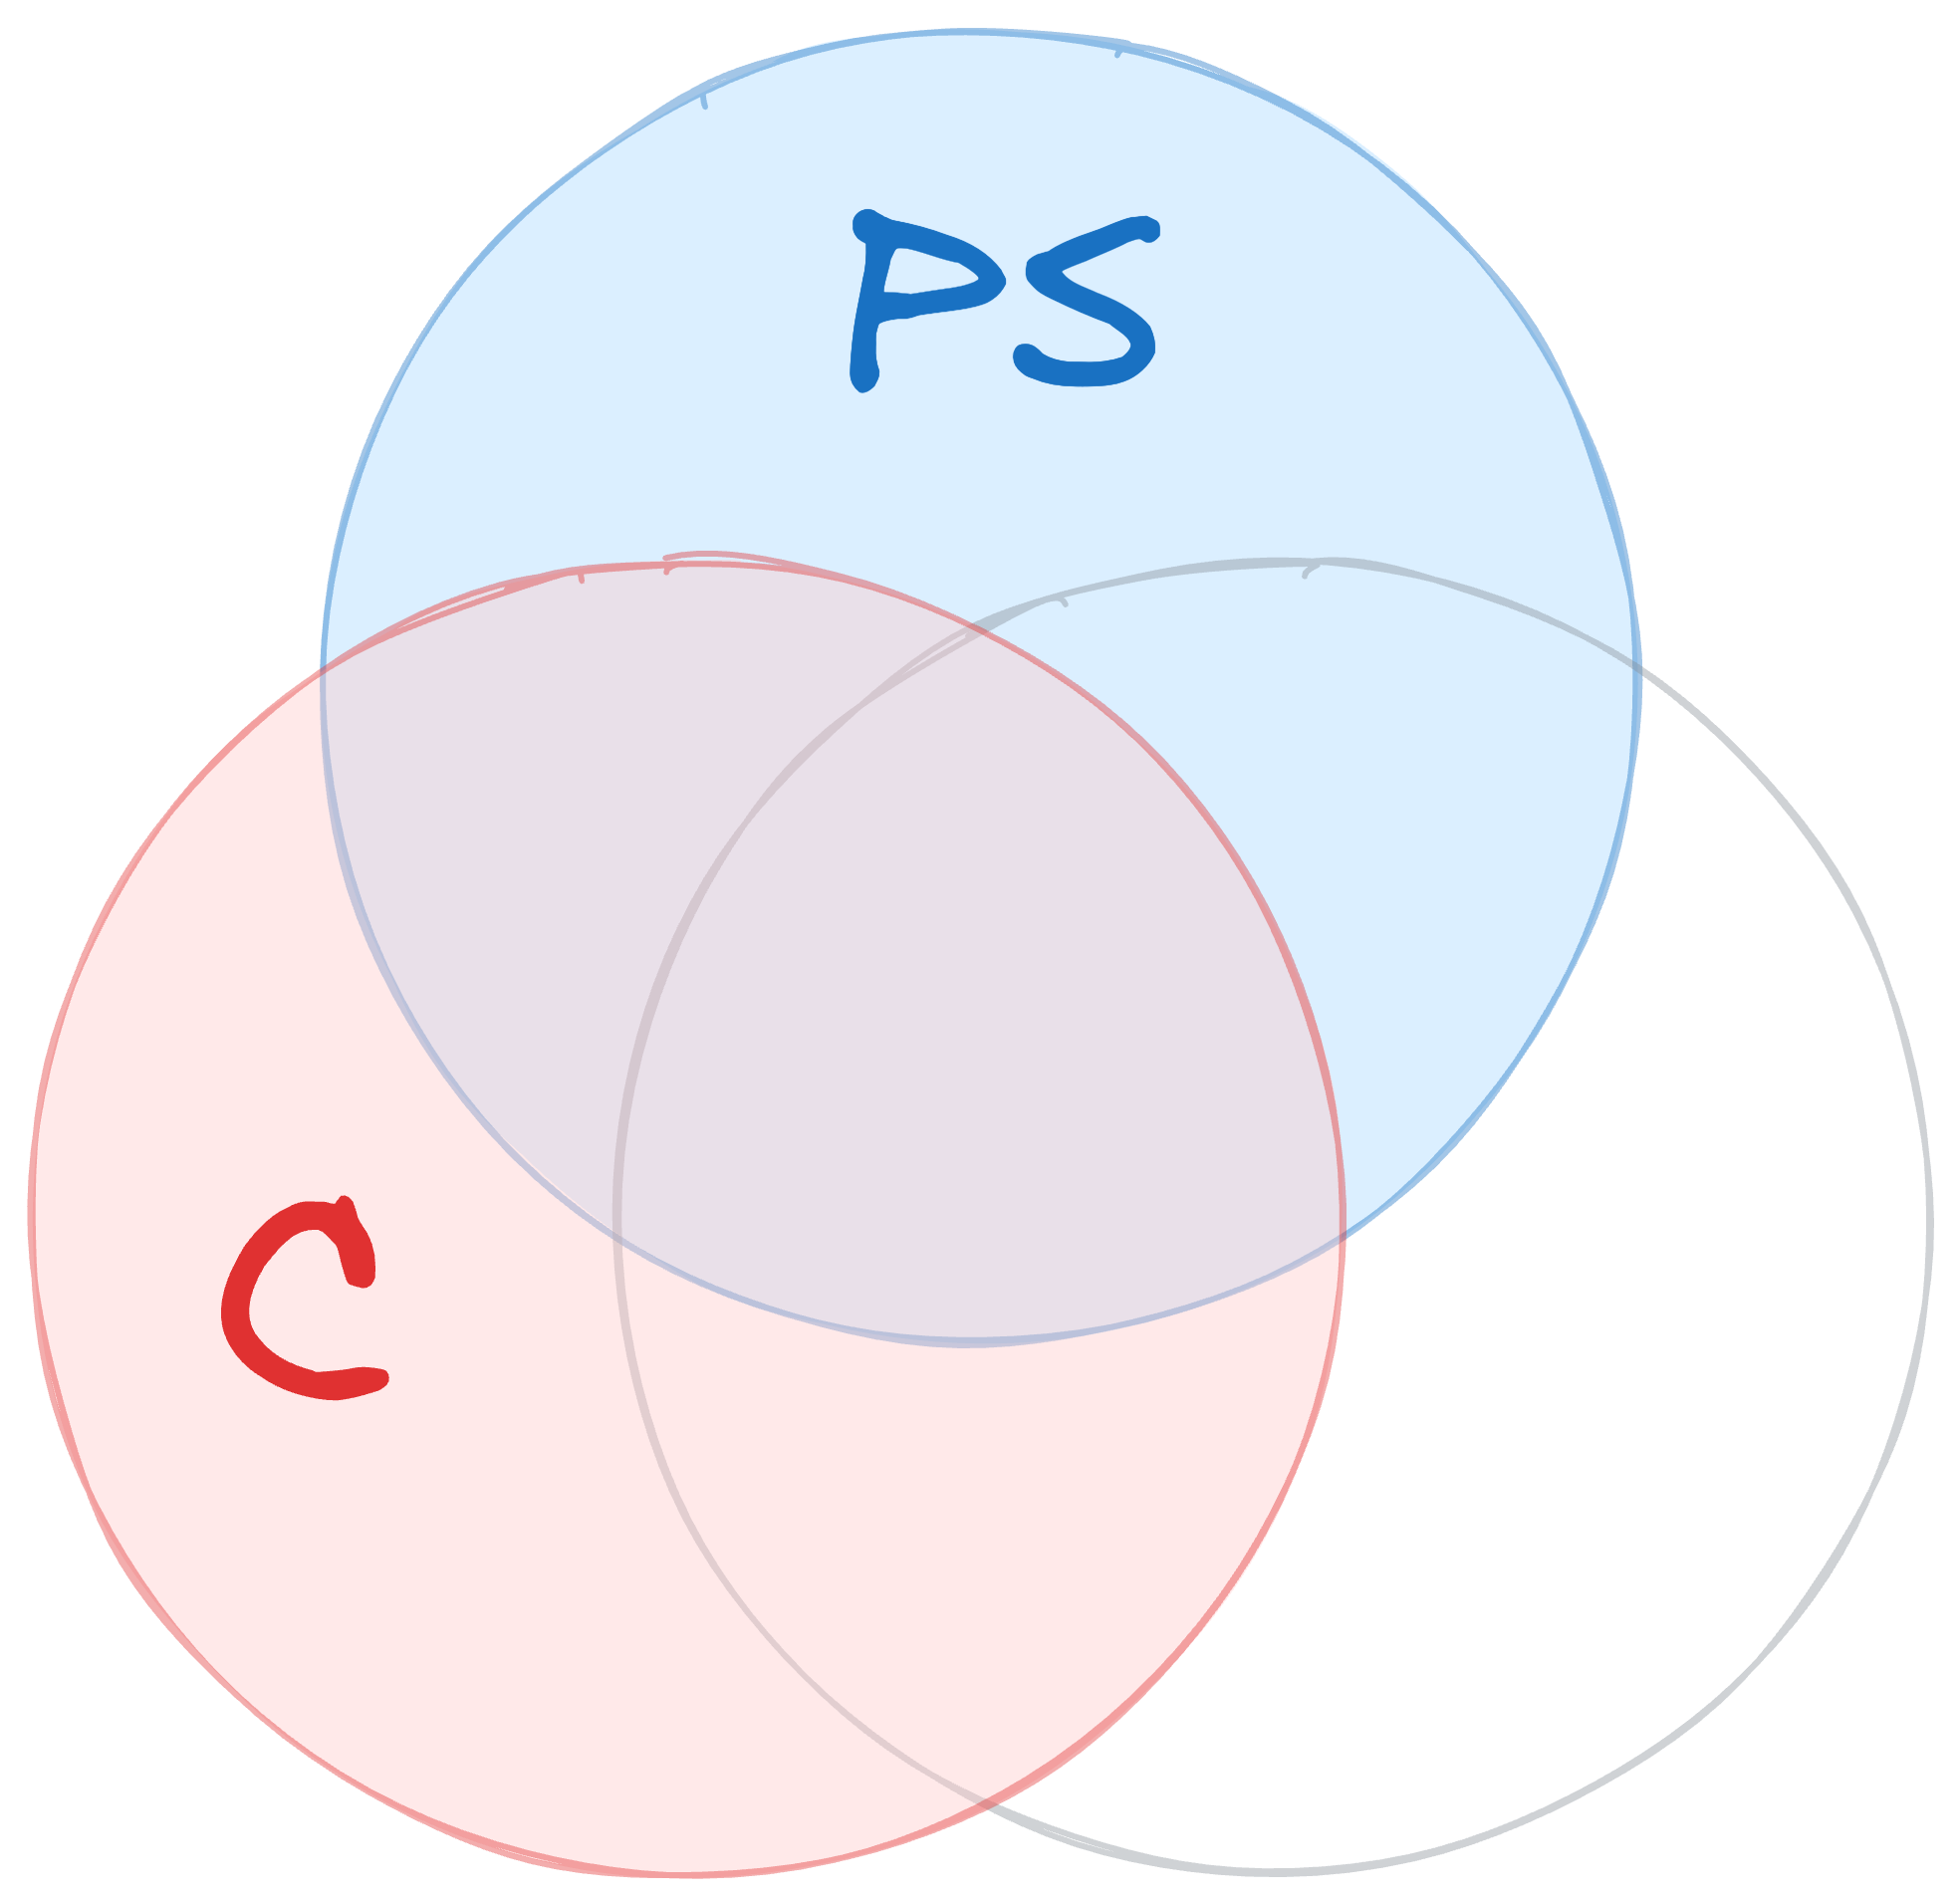
\includegraphics[width=\marginparwidth]{Figures/topics_ctrl_ps.png}
}
\label{sec:controlPartiallySpecified}

% Types of partial specification
The notion of \emph{partial specification} plays a central role in this thesis, and it appears in various forms within discrete system modeling. Broadly speaking, partial specification refers to situations in which some aspects of a system's structure or behavior are unknown, undefined, or only partially observable. This incompleteness poses a unique challenge for control, as it requires strategies that remain effective despite the inherent uncertainty. In the following paragraphs, we discuss several interpretations of partial specification and their relevance to Boolean network control.


% Non-observability
\emph{Non-observability} is considered to be one of the forms of the partial specification, since in such systems, the current state of the system cannot always be determined precisely~\cite{Kalman1960}. This challenge has long been recognized in control theory~\cite{Flokentin1962, Sorenson1968}, as we can not optimize control for the source state (because it is unknown). Non-observability is particularly common in biological systems where the full internal state is often hidden, or changing too rapidly to measure.~\cite{Liu2013,Villaverde2019} In the context of Boolean networks (BNs), we adopt a similar view: the internal dynamics are considered unobservable, and only attractors (i.e., stable, long-term behaviors) are assumed measurable. This abstraction is essential in biological modeling, where stable phenotypes correspond to observable steady states. Nonetheless, this thesis is concerned with an even broader and more complex notion of partial specification.


% Non-determinism
Another important source of uncertainty is \emph{non-determinism}, especially relevant in asynchronous BN. In such systems, the exact transition path from one state to another is not deterministic — multiple successor states may exist. This lack of transition determinsm can be viewed as a form of partial specification, as it obscures the system’s exact evolution over time. However, in this thesis, we treat non-determinism as an intrinsic property of the system rather than as an imperfection in its specification. The control task must therefore account for all possible transitions, ensuring control guarantee across all potential execution paths.


% Game theory, Mandon
Nondeterminism also inspired a game theoretic interpretation of control. In this perspective, the system and its uncertain evolution are viewed as an adversarial player, and the controller must identify a winning strategy to guide the system to a desired state~\cite{Mandon2019PHD}. This view is particularly useful in multistep control problems, where strategies unfold over multiple transitions and must remain effective despite adversarial behaviors. While the game theoretic approach provides valuable conceptual insight, the focus of this thesis lies in simpler control settings (e.g., single-step or permanent control), where the full strategy does not need to be explicitly constructed.


% Multiple possible functions 
A more structural form of partial specification arises in models such as \emph{probabilistic Boolean networks} (PBNs)~\cite{Shmulevich2002}, where uncertainty is introduced by allowing each variable to be governed by multiple update functions, each with an associated selection probability. In such models, not only is the update time of variables uncertain, but so is the logic guiding those updates. Thus, control must operate over a probability-weighted ensemble of behaviors, further complicating the synthesis of effective system perturbations.

In contrast, the \PBN{} framework central to this thesis allows each variable to have multiple possible update functions, but crucially assumes that only one “true” function per variable governs the evolution throughout the system's runtime. That is, while the identity of the function is unknown (and remains hidden due to nonobservability), it is assumed fixed. The resulting dynamics are therefore equivalent do asynchronous BN under a hidden function instance, though unknown from the observer’s perspective. This hybrid interpretation combines partial structural knowledge, non-determinism, and limited observability, creating a novel challenging control problem that this thesis aims to address.

% Partial functions?

% Control of other partially specified discrete systems?
% The control of partially specified systems is also closely related to the broader framework of discrete event systems (DES), where uncertainties arise in timing, event ordering, and transition logic. Similar challenges are present in stochastic models such as Markov chains and probabilistic transition systems. These models share structural affinities with PBNs, particularly in how transitions are defined over distributions rather than deterministic rules. These are a few examples which were inspiration for development of the BN. Now let's focus on the control of BN and methods closer to our approach. 



\section{Control of synchronous Boolean networks} 
\label{sec:controlSynchronous}
\marginpar{
    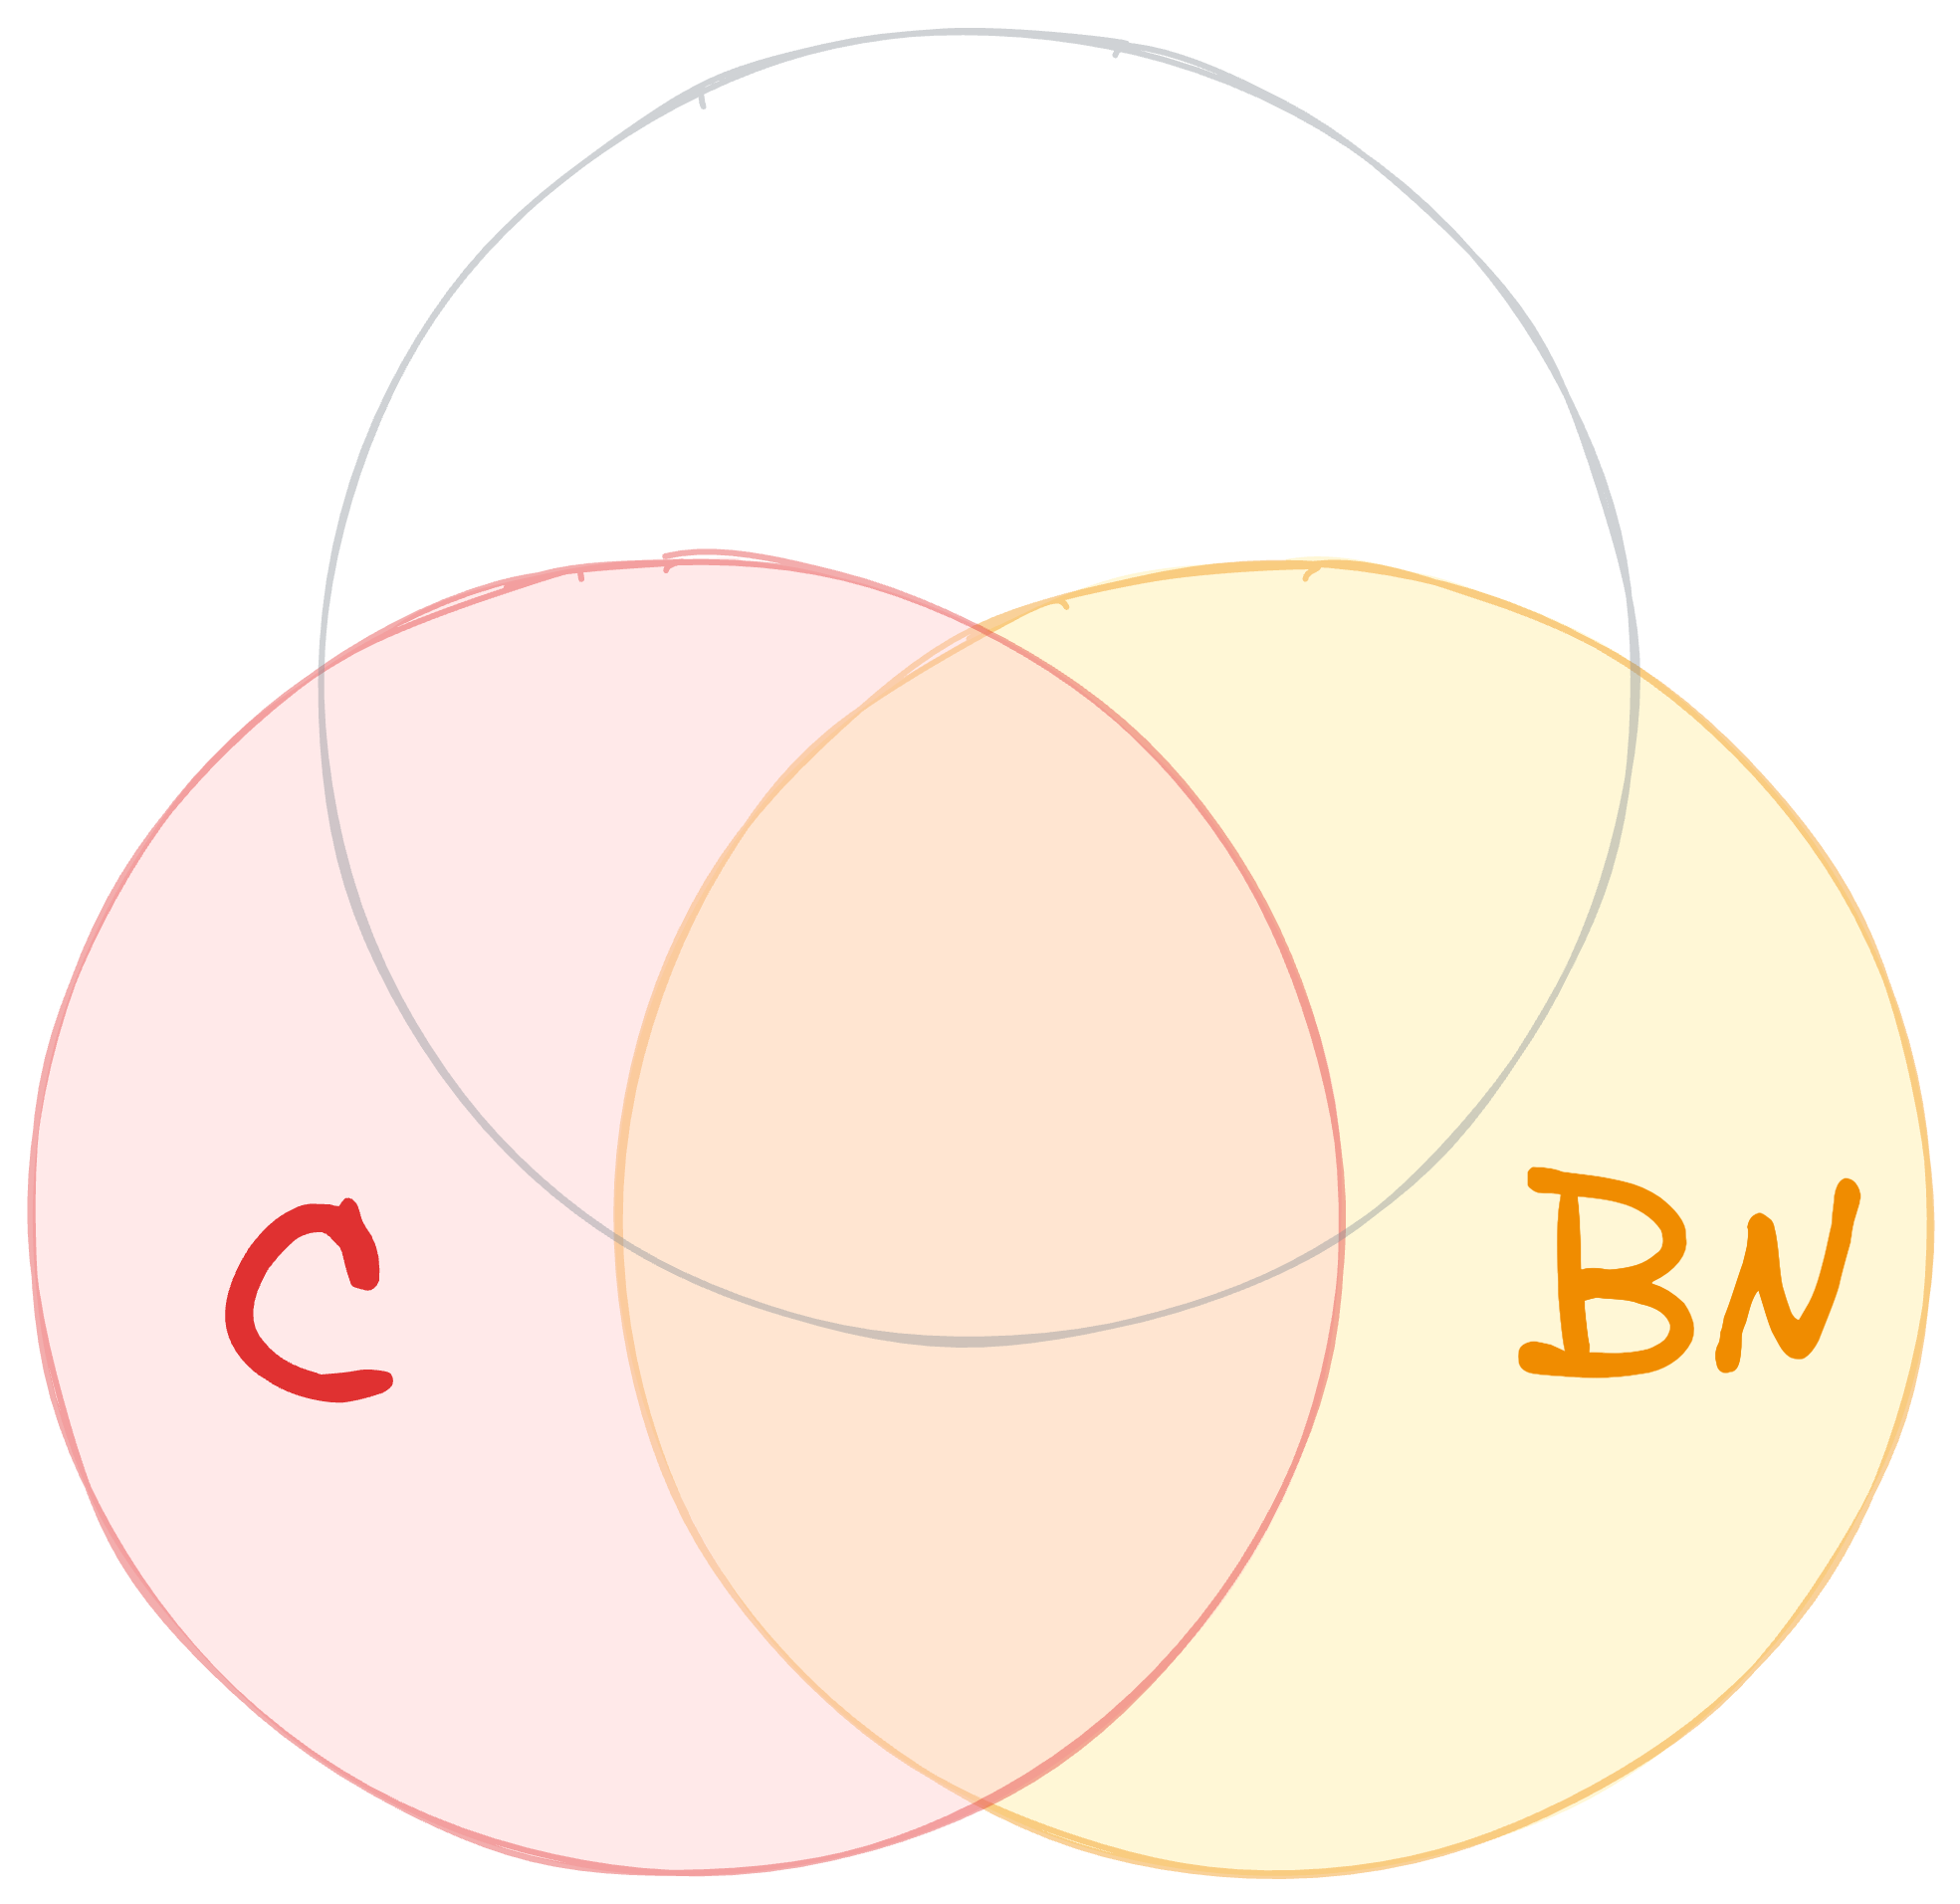
\includegraphics[width=\marginparwidth]{Figures/topics_ctrl_bn.png}
}
% Control of synchronous networks
Synchronous Boolean networks are characterized by the \emph{simultaneous} update of all variables at each time step. This deterministic update scheme ensures that the system's evolution is fully determined by its initial state. Despite this determinism, research on control for synchronous BNs remains highly relevant, especially because it provides foundational insights and inspiration for tackling more complex cases, such as asynchronous or partially specified networks.

% BCN relationship
As discussed earlier, control of Boolean control networks (BCNs) represents the most basic form of  BN control. In BCNs, control inputs can be modeled as direct perturbations of network variables or update rules. Therefore, if one enumerates all possible perturbations as  BN inputs and adjusts update functions accordingly, BCN-based control can trivially solve the control problem for synchronous BNs. Nonetheless, this naive approach is exponentially complex. Moreover, despite the deterministic underlying dynamics, the control problem for synchronous BN remains computationally challenging as it was proven to be NP-hard~\cite{Akutsu2007}.

% ASP
Given the Boolean nature of BN, an interesting problem reduction to the \emph{answer set programming} (ASP) was explored in~\cite{Kaminski2013}. The encoding of the problem here is quite straightforward, as the BN can be represented as a logic program, the control problem is formulated as a query, and even perturbations can be expressed as additional rules very conveniently by using three-valued logic. The approach was proven efficient, being handle to solve BN with up to 200 variables and perturbation size 10. A slightly generalized approach was later developed, allowing to specify general changes in long-term behavior (as opposed to output behavior only). Finally, ASP was also used to not just control the BN but also to infer input-output experiments and design therapeutic targets also packaged as a tool caspo~\cite{Videla2014,Videla2017}.

% One-step control
Beyond basic control problem, several more refined problem variations have emerged over time. Notably, Kim et al.~\cite{Kim2013} introduced the notion of a \emph{control kernel}, which is defined as the minimal set of variables that need to be set \emph{initially} in order to drive the system toward a desired attractor. This formulation corresponds to a one-step control problem and is closely aligned with the concept of perturbation strategies discussed in \autoref{subsec:perturbations}. 

% Phenotype control
Another perspective is provided by Choo et al.~\cite{Choo2018}, who generalized the target of control from a specific attractor to a broader \emph{phenotype}, defined as a set of target states sharing functional or biological characteristics. This abstraction reduces the granularity of control targets and allows for more flexible solution spaces. While computationally simpler than controlling asynchronous or partially specified networks, phenotype-based control provides valuable conceptual tools. Indeed, as discussed in \autoref{chapter:phenotype_control_psbn}, a similar generalization is central to our own contributions in control of \PBN{}.

% Ensembles control
A particularly relevant concept introduced for synchronous BNs is the control of \emph{Boolean network ensembles}~\cite{Gates2016,Correia2018,Gates2021,Videla2017}. In this setting, one considers a family of networks with identical topology but differing update functions. The control problem becomes finding a perturbation that guarantees convergence to the same attractor across all network instances. This notion aligns closely with the challenges posed by partial specification as we will see later in this work.

%Our own approach, presented in \autoref{chap:source_target_control}, generalizes this idea by relaxing the requirement for perturbations to strictly control every possible instance. This enables a framework for \emph{control-guided network inference}, as will be elaborated in \autoref{X}.

% Attractor computation
Finally, synchronous dynamics can also serve as a useful tool for analyzing asynchronous networks. Specifically, attractors identified under synchronous updates can act as approximations or partial indicators of stable attractors in the asynchronous setting~\cite{Zheng2013}. While this correspondence is limited to certain classes of attractors (e.g., stable fixed points), it provides valuable structural insights that can guide further analysis of asynchronous dynamics.


\section{Control of asynchronous Boolean networks} 
\label{sec:controlAsynchronous}

At the beginning of writing this thesis, the closest related work was the control of asynchronous BN~\cite{Smijakova2020}. Asynchronous BN offer a more biologically realistic modeling framework, as they incorporate asynchronous variable updates~\cite{Chaves2005}. This added expressiveness, however, introduces significant challenges for control, since the system's evolution is no longer deterministic and may follow multiple trajectories from the same initial state. To address this complexity, a broader variety control techniques were developed. In the following subsections, we survey key approaches to the control of asynchronous BN, highlighting the methods employed, the types of perturbations considered, and the formulation of control objectives.


\subsection{Refined strong basins search} \label{ss:strongbasinidentification}

Another branch of methods solving the BN control problem is based on the efficient identification of the strong basin of a target attractor (see \autoref{ss:state_space_structures}). By definition, a strong basin is the maximal set of states from which only the given attractor is reachable. Once the strong basin is identified, the control task reduces to finding the minimal perturbation that drives the BN into this basin. This is effectively a solution to the source-target control problem using one-step perturbations, since the solution there is as trivial as finding a state from strong basin with minimal Hamming distance to the source state. However, when considering other types of perturbations (e.g., temporary or permanent), additional computational steps are needed to determine appropriate control strategies.

A trivial approach to identifying the strong basin is through a fixed-point algorithm: nodes are iteratively removed from the weak basin if they have transitions that lead outside the basin. When no such nodes remain, the resulting set constitutes the strong basin. While conceptually simple, this method does not scale well for large biological networks. To address this limitation, a more efficient algorithm was proposed by Paul et al.~\cite{Paul2018BCB}, based on a decomposition of the state-transition graph (STG) into blocks.

The core idea of this block-based method is to partition the STG into basic blocks, where each block consists of a strongly connected component and its parent states. These blocks are considered in partial projections of the BN (subsets of the full variable set). Once identified, the blocks are topologically sorted and then unfolded, starting from the block containing the attractor, until all states in the strong basin are identified.

Compared to the stable motif approach that was discussed previously, strong basin identification must be performed separately for each target attractor when solving more complex variants of the control problem, such as full-control or all-pair control. Nonetheless, for smaller BN, the decomposition-based method has shown better performance even in full-control scenarios~\cite{Paul2018CMSB}, whereas for larger networks, the stable motif-based method tends to remain more efficient.

The strong basin identification approach has been successfully applied to source-target control with a variety of perturbation types: one-step initial perturbations~\cite{Paul2018BCB, Paul2018CMSB}, temporary and permanent perturbations~\cite{Su2019FM}, and sequential (attractor-based) variants~\cite{Mandon2019CMSB, Su2020}. More recently, the method has been extended to support target control under all types of perturbations~\cite{Su2020BCB,Su2020phd}. All of these techniques have been integrated into the software toolkit CABEAN~\cite{Su2020Bioinformatics}, facilitating broader adoption and experimentation.

\subsection{Stable motifs identification} \label{ss:stablemotifidentification}

Some techniques address complexity of asynchronous BN by analyzing only RN along with the update functions at first. The obtained information can be used to dramatically reduce the size of explicit state space, which needs to be explored to solve the BN control problem. 

One such approach is based on identification of \emph{stable motifs}~\cite{Zanudo2013,Zanudo2015}. A stable motif is a subset of variables and their corresponding values that, once reached, remain unchanged indefinitely. By identifying all stable motifs, one can construct a so-called \emph{succession diagram} that captures all possible nondeterministic runs of a BN. This diagram provides a structured way to navigate through the system's dynamics and determine the appropriate interventions needed to reach a desired attractor.

The strength of this method lies in its global topological analysis, which enables efficient performance. Once stable motifs are identified, they can be reused to compute control strategies for any attractor within the BN. This facilitates a solution to the full-control variant of the problem and offers valuable insights into the system robustness. However, the method is not complete as it may miss some viable control strategies. Additionally, stable motifs primarily serve as guidance for control design and must be validated through simulation to confirm their effectiveness. This validation also determines whether the required perturbations should be applied transiently (temporarily) or permanently.

To support broader adoption, the method was later implemented as a Python package, significantly improving its performance as well as accessibility for the research community~\cite{Rozum2022}.

\subsection{Trap spaces} 
\label{ss:asp}

Another approach based observing partially stabilized components is based on observing so-called \emph{value percolations}. This phenomenon is observed if we generalize successor function from a single state to subspaces. This way we can very quickly trace how the reachable subspaces from a given perturbation. Such an approach was first employed by aforementioned approach for the synchronous BN~\cite{Krumsiek2011,Videla2017}.

The downside of potential percolation-only approach for asyn\-chro\-nous BN is that it is not complete, since it does not guarantee to discover all perturbation strategies. Therefore, it was extended later by combining percolations with trap spaces exploration~\cite{Fontanals2020}. Trap spaces are spaces of the BN which can not be left once reached (see \autoref{ss:state_space_structures}). 

Compared to the strong basin, however, if we find a trap space in a \emph{synchronous} BN, the trap spaces are also contained in network's \emph{asynchronous} dynamics. Therefore, we can transfer the knowledge obtained from analysis of a simpler dynamics of synchronous BNs and use it for computing control of asynchronous BNs. The perturbations used in this approach are temporary state perturbations. 

Since the target of the method is a trap space, the target of the control is also generalized from a single attractor to an arbitrary subspace. This way the method is able to solve the control problem for a wider range of targets (attractors), and allow for more flexible control strategies. 

Given the nature of percolations and trapsaces, similar to the synchronous BN approach which inspired this work~\cite{Krumsiek2011}, methods for control of asynchronous BNs also use ASP to compute the control strategies. 

What is also interesting is that logical programming allowed to express the other types of perturbations than just variable perturbation, but also \emph{edge} perturbations, which disable a regulation of one variable to another~\cite{Fontanals2022c,Fontanals2023}.

It is worth mentioning, that there is also a significant body of work focusing solely on efficient computation of trap spaces. Therefore, tools and methods such as PyBoolNet~\cite{Klarner2018}, BioLQM~\cite{Naldi2018}, trappist~\cite{Trinh2022}, or tsconj~\cite{Trinh2024} can inspire future research of control methods.

\subsection{Model checking}
\label{ss:model_checking}

The methods based on percolation and trap spaces were limited to a specific subspace target (i.e., not a combination of multiple independent subspaces). Moreover, they needed to be combined with other approaches in order to obtain a complete solution to the control problem. These caveats inspired the development of a new method based on the model checking approach~\cite{Fontanals2022b}. 

The model-checking approach is using CTL to easily express the control problem. Nonetheless, the general model-checking approach tends to be slow since it explores the entire state space to make sure, that all states fulfill the properties.

Therefore, the control method itself is based on the idea of using a model checking as a ``backup'' approach if we are unable to assess whether a control strategy works using the trap-space-based method introduced previously. This way we obtain both, high performance for the majority of the cases and a complete solution for the rest.


\subsection{Other techniques}
Finally, we describe other techniques to control asynchronous BN which do not fit into the previous categories, because they use less conventional or a combination of multiple methods.

Kali is a tool for performing in silico therapeutic target discovery using network attractors~\cite{Poret2014,Poret2017,Poret2018}. The tool was in its last version updated to handle asynchronous and multivalued BNs. 

In this approach, the input is a physiological variant of the network and a pathological variant of the network. The goal is to find perturbations that drive the pathological variant to behave like the physiological one, i.e., to reach the same or at least a subset of the same attractors.

The approach is based on a combination of several techniques. First, the tool identifies all attractors of the BN using random walks. Then, so-called \emph{therapeutic bullets} candidates are generated, using uniform distribution of all possible options. These are combinations of ``bullet targets'' (states where perturbation is applied) and ``bullet values'' (the values to which the targets are perturbed).

The candidates are then evaluated by simulating the BN with applied bullet targets. The evaluation is based on the proportion of initial states reaching a physiological attractor or a portion of reachable physiological attractors in case of synchronous BN.

An interesting aspect of the method is, that not only universal perturbations are computed, but also \emph{existential} perturbations evaluated and quantified. Also, the method is focused on refining a model with the same behavior as opposed to driving it towards a specific static set of states. On the other hand, the method is not complete, since it relies on random walks to identify attractors and evaluate perturbations.

Another recently developed approach relies on semi-tensor products~\cite{Su2024}. This is another example of successful generalization of a technique working on synchronous BNs to asynchronous BNs. 
Again, given the nature of semi-tensor products, the control is achieved using periodical impulsive control. The viable controllers are defined along with the model, similarly to the synchronous BCNs mentioned in \autoref{sec:controlSynchronous}. 

Nonetheless, in this approach, the controllers do not need to be just static Boolean values, but can be also dynamic components that are gaining the value periodically. Moreover, this approach is able to quantify probability of reaching the target states as opposed to inevitably reach the state after applying the control.

\section{Control of most-permissive Boolean networks}
\label{sec:controlMostPermissive}

The previously described variants of BNs are limited in their ability to capture certain biologically significant behaviors~\cite{Pauleve2020}. For example, none of the earlier models can accurately represent the incoherent feed-forward loop of type 3 (I3-FFL)~\cite{Mangan2003}, a well-known motif in gene regulatory networks.

Most-permissive semantics enhances the expressiveness of BNs by allowing transient dynamics during state transitions from 0 to 1 and vice versa. This feature enables the representation of intermediate states, capturing subtleties in biological processes that are not strictly binary.

A major motivation for the development of most-permissive semantics lies in its application to model inference. The aim of model inference is to narrow down a broad set of candidate models to those that accurately reflect observed biological behavior. Under more restrictive Boolean semantics, correct models may be incorrectly discarded due to the absence of valid trajectories leading to experimentally observed attractors. As the name implies, most-permissive semantics allow the widest range of behaviors, thereby reducing the risk of false negatives during model selection.

An additional advantage of most-permissive Boolean networks is that despite their increased expressiveness they remain analytically tractable. In particular, Answer Set Programming (ASP) has proven to be well-suited for this framework, as it naturally supports the declarative encoding of Boolean logic and allows efficient searching for trajectories that either confirm or refute specific hypotheses~\cite{Pauleve2020}. However, a notable limitation of this approach is the difficulty in analyzing quantitative properties, such as the size of basins of attraction. For such purposes, simulation-based methods may be used, though they typically trade off completeness and performance~\cite{Roncalli2022}.

The tool BoNesis integrates various techniques for the analysis of most-permissive Boolean networks, including simulation, attractor detection, model synthesis, and control~\cite{Pauleve2023}. For symbolic reasoning it leverages ASP, enhanced with counterexample-guided abstraction refinement (CEGAR)~\cite{Riva2023}, while simulations of network dynamics are performed using an iterative depth-bounded approach.

Control within BoNesis is guided by specifying biological markers, which semantically correspond to the phenotypes introduced in \autoref{ss:model_checking}. The perturbations computed by the tool are permanent, and the control is universal, meaning that the desired properties must hold across all possible runs of the Boolean network. To minimize the size of the required perturbation set, users can optionally specify an initial configuration, thereby avoiding over-optimization across all possible initial states.

BoNesis supports differentiated control strategies for steady states (fixed points), and all attractors, enabling optimization tailored to task complexity, since reprogramming steady states is typically less computationally intensive~\cite{Pauleve2023}. Another notable feature of BoNesis is its ability to control ensembles of Boolean networks, which is especially relevant since model inference usually produces a set of plausible models rather than a single one. When controlling BN ensembles, users can choose between existential and universal control strategies. Existential control identifies perturbations that succeed in at least one model in the ensemble, while universal control yields perturbations that are guaranteed to work across all models.

\section{Leveraging control for model refinement}
\label{sec:controlInference}
\marginpar{
    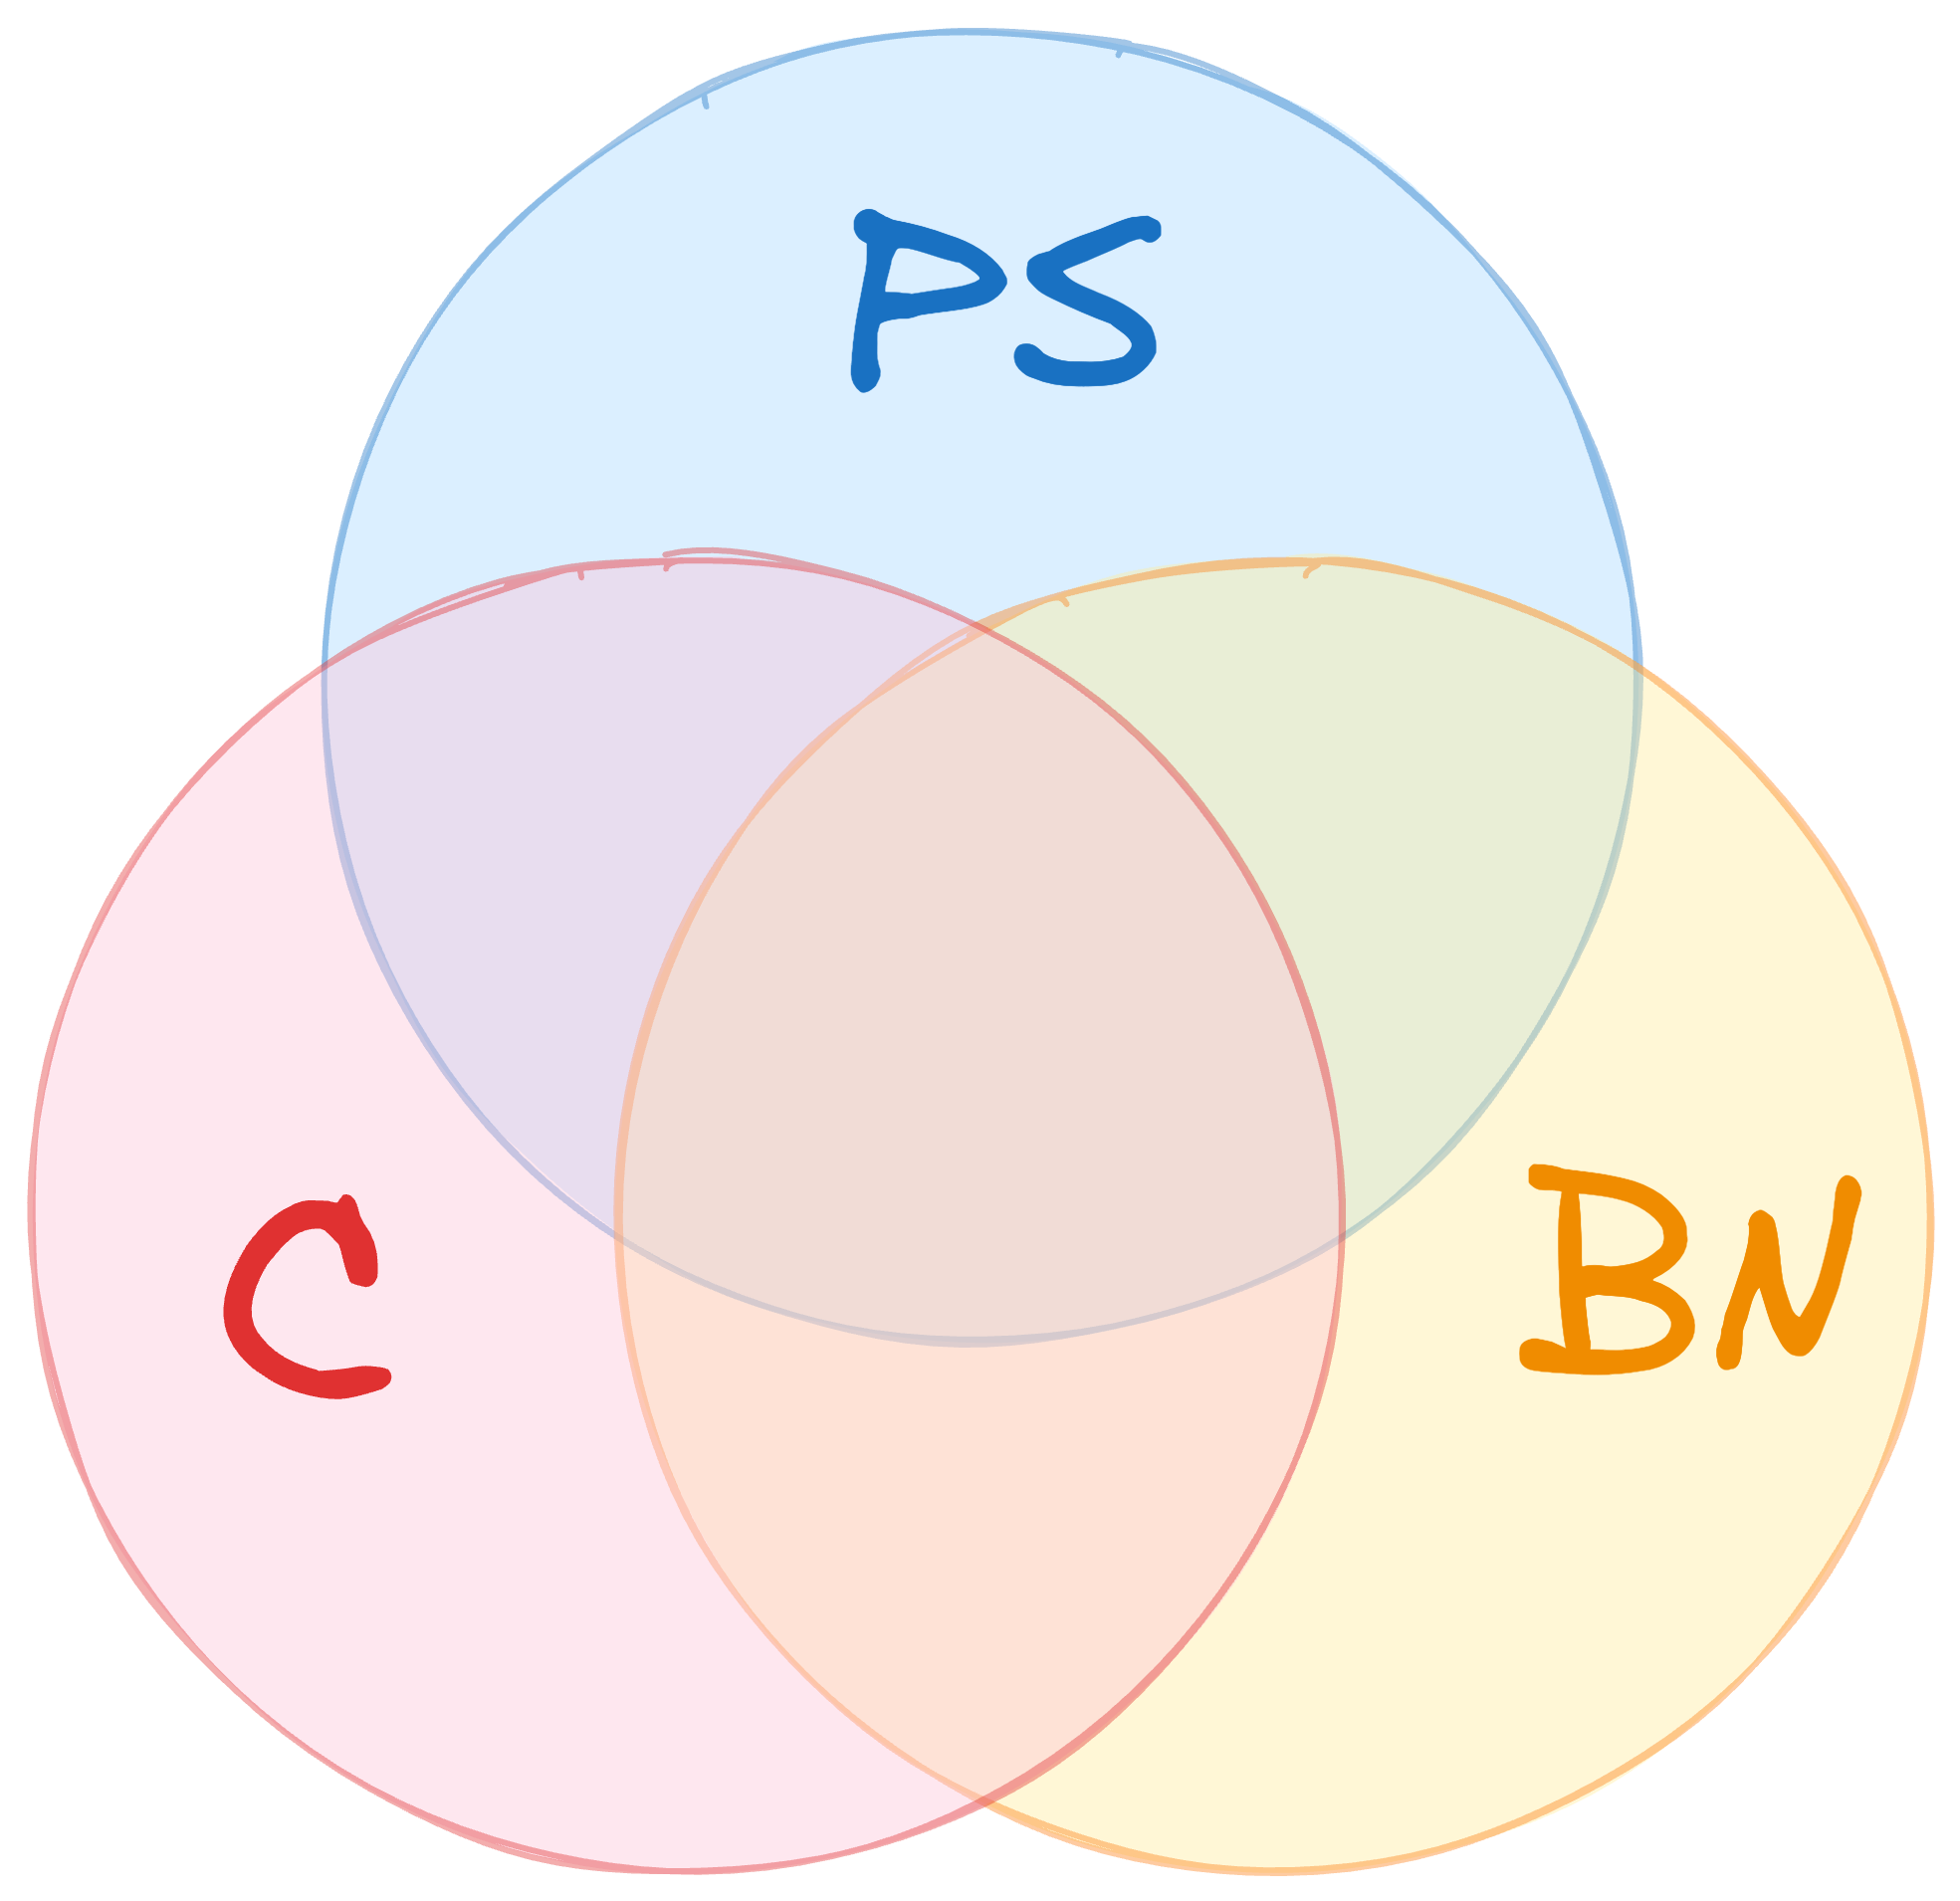
\includegraphics[width=\marginparwidth]{Figures/topics_all.png}
}

Traditionally, the control of Boolean networks has been viewed primarily as a means to modify system's  behavior, most notably for applications such as cellular reprogramming. However, recent research has begun to explore control as a valuable asset in the model refinement process. In this context, control can serve several important purposes:

\begin{enumerate}
    \item Handling uncertainty: Model inference may produce many network models that all fit the data. A good control strategy should work across these variations. If control leads all plausible models to the same desired behavior, it increases our confidence in both the models and the control itself~\cite{Chevalier2025}.
    \item Model verification: Control does not need to be just a downstream consumer of inferred models; it can also act as a verification tool. By applying perturbations and comparing the system's behavior to experimental observations, we can check that the model behaves in accordance with observations.
    \item Guiding experiments: When experimental data is limited or if there is an abundance of plausible models, control can help design better experiments. It can identify the most informative perturbations; those that produce system behaviors revealing how the network works.
\end{enumerate}

A growing body of work focuses on integrating perturbation data such as gene knockouts and over-expression experiments into the model inference pipeline~\cite{Gjerga2020,Yordanov2016,Park2025}. These efforts often rely on analyze model ensembles to explore the impact of perturbations. For instance, logic-based approaches can use Satisfiability Modulo Theories (SMT) to impose constraints on system dynamics, enabling the prediction of perturbation effects and facilitating model refinement based on experimental evidence~\cite{Yordanov2016}.

Control can also help prioritize new experiments by running in-silico simulations to predict which experiments would be most useful for refining the model. This idea originally came from continuous models, where system analysis has been used to design experiments that help fine-tune model parameters~\cite{Kreutz2009, Melykuti2010}. Later, similar strategies were applied to regulatory networks, where perturbation experiments were designed specifically to uncover the network's underlying structure~\cite{UdDean2016}.

Similar strategies have been developed for BNs, though with varying degrees of generality and scalability. Early works addressed experiment design for synchronous Boolean networks~\cite{Videla2015}. However, the only refined parts are inputs and outputs of the network, thus all available perturbations need to be included into model inputs beforehand.

Another line of work concerned with perturbations experiment design uses a maximum entropy framework to choose experiments that provide the most information~\cite{Atias2014}. Still, these methods rely heavily on simulations and are expected to be hard to scale; especially when dealing with asynchronous dynamics, where the number of possible system behaviors grows rapidly.


\section{Related tools}
\label{sec:relatedTools}

The majority of previously introduced methods were encompassed as software tools in order to make them accessible to a wider audience. Given the numerous nuances between control problems it is not an easy task to exhaustively compare the tools between them. Moreover, some features combinations might not be available. 

\begin{table}[]
    \label{tab:tools_compare}
    \centering
    \scalebox{0.8}{
    \begin{tabular}{rccccccl}
    \textbf{Tool} & \rot{\textbf{Source-targ.}} & \rot{\textbf{Target}} & \rot{\textbf{Phenotypes}} & \rot{\textbf{Partial spec.}} & \rot{\textbf{Pert. types}} & \rot{\textbf{Complete}} & \textbf{Main method} \\
    CABEAN  & ? & x & X & X & X & X & Strong basin search, ASP \\
    BoolNet & ? & x & X & X & X & X & X \\
    KALI    & ? & x & X & X & X & X & X \\
    CASPO   & ? & x & X & X & X & X & X \\
    BoNesis & ? & x & X & X & X & X & ASP \\
    AEON    & ? & x & X & X & X & X & BDDs, Symbolic 
    \end{tabular}
    }
    \caption{Comparison of related software tools for Boolean network control.}
\end{table}

\section{Summary}
\label{sec:sota_summary}



 
\chapter[Source-target control of PSBN]{Source-target control of partially specified Boolean networks}
\marginpar{
    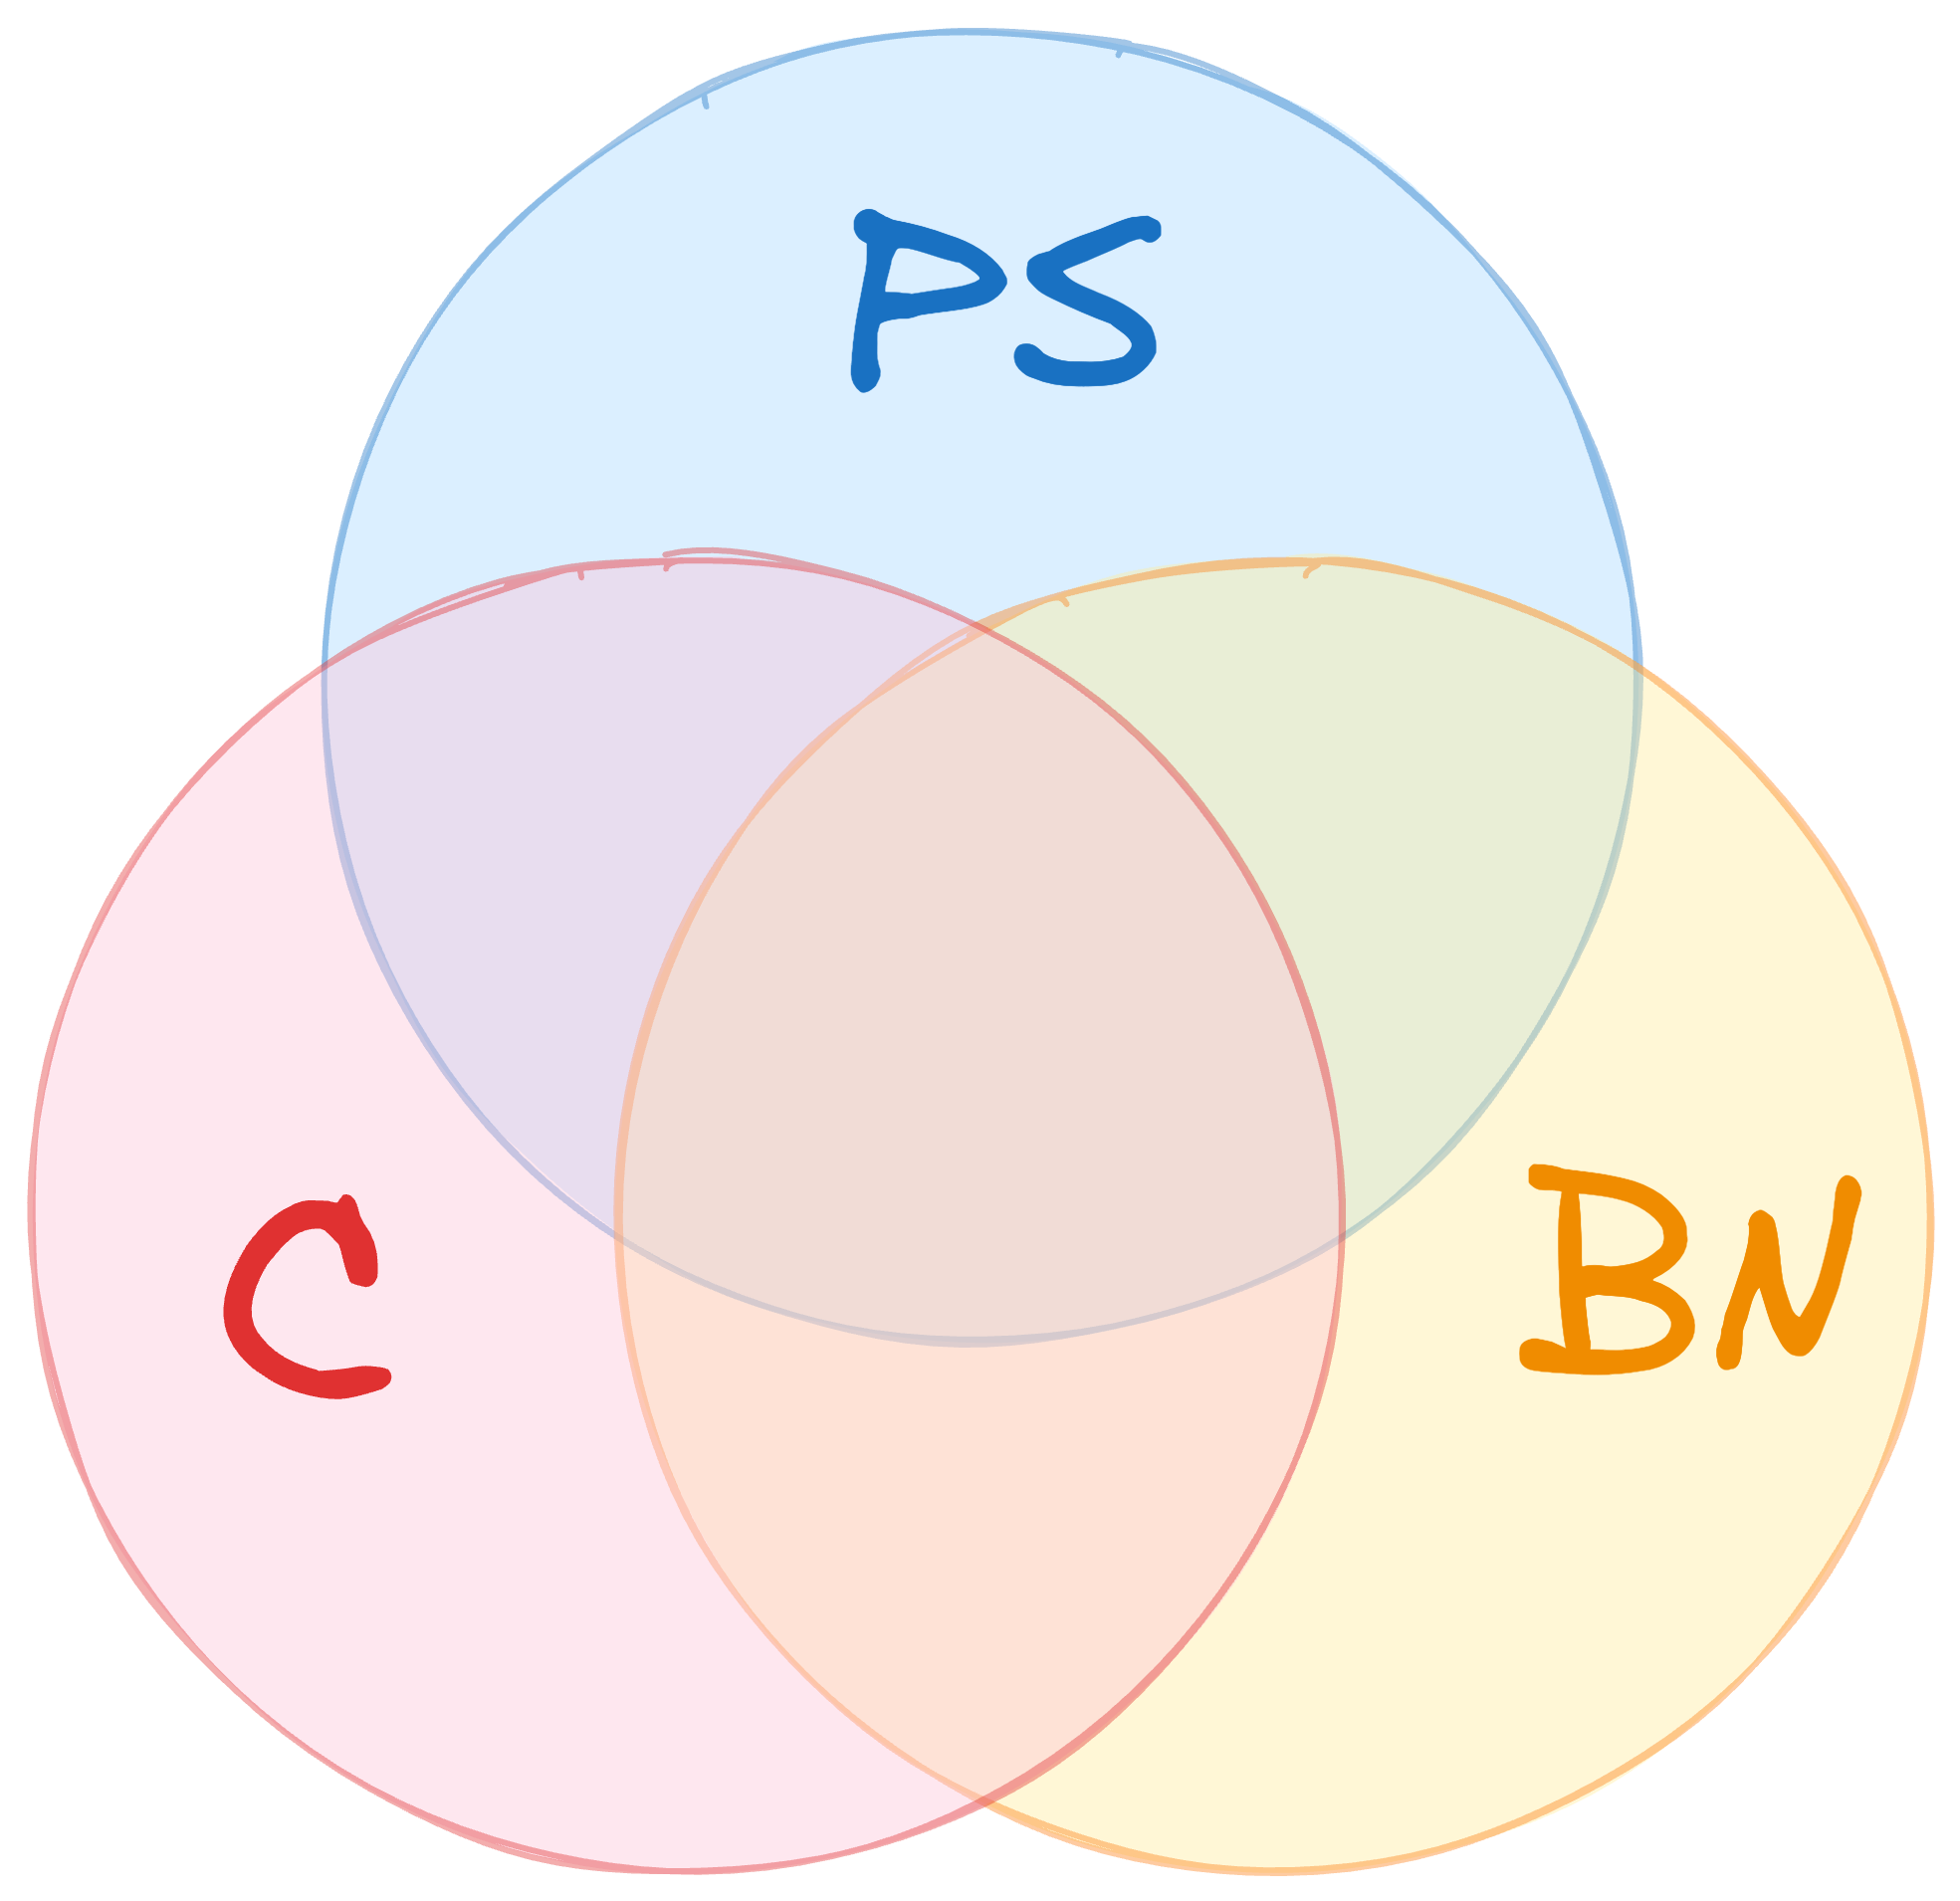
\includegraphics[width=\marginparwidth]{Figures/topics_all.png}
}
\label{chapter:source_target_control}

In our work, the source-target control problem provides a natural starting point for the development of control methods and for understanding the challenges arising from the partial specification of Boolean networks. Since the source state is fixed, it is not necessary to analyze the effect of a perturbation on the entire state space; instead, the search for suitable perturbations can be optimized for the given initial state.

We begin with one-step perturbations, which constitute the simplest class of interventions. As will be shown later, computing one-step perturbations is significantly easier than computing permanent or temporary perturbations, because it does not require modifying the transition system of the network to account for sustained intervention.

However, one-step perturbations are often less efficient than perturbations applied over a longer time horizon. Therefore, we also develop methods for permanent and temporary perturbations, which are computationally more complex but may yield smaller perturbation sets.

In this chapter, we first define the source-target control problem in \autoref{s:source_target_problem_definition}, including the notions of one-step, permanent, and temporary perturbations. Next, in \autoref{sec:target_semisymbolic}, we present a symbolic method for computing one-step source-target control in partially specified Boolean networks. Finally, in \autoref{sec:ostp_symbolic}, we extend this method by representing the state space of perturbed networks so as to handle permanent and temporary perturbations as well.


\section{Problem definition}
\label{s:source_target_problem_definition}

The cardinal difference between classical Boolean networks and partially specified Boolean networks is that the latter can be interpreted in many ways, depending on the chosen parameter valuation. As a consequence, the state transition graph of a PSBN is not uniquely defined. Instead, every interpretation induces a different instance of the PSBN, which in turn induces a different state transition graph.

On the other hand, the definition of a perturbation is independent of the network's parametrization. A perturbation simply fixes the values of certain variables to constants. Therefore, the definition of a perturbation is very similar to the one used in classical Boolean networks. 

What we need to keep in mind, however, is the effect of a perturbation on the network's transition system. In a classical Boolean network, a perturbation can be applied to the whole state space, and it simply removes all states that are not admissible by the perturbation. In a PSBN, however, the effect of a perturbation can differ between different interpretations. This is because the unperturbed variables can still evolve freely. As a result, a perturbation can achieve control for some interpretations, while failing for others.

\subsection{Perturbations}

Here, we build on the definitions of perturbations and their applications from the previous chapter. Most notably, we will leverage the concepts of perturbation (\autoref{def:perturbation}), application of a perturbation to a source state (\autoref{def:perturbation_application}), perturbation application to a state-transition graph (\autoref{def:perturbed_stg}) and a perturbed run of a Boolean network (\autoref{def:perturbed_run}).

Now, let us remind the definitions of a perturbation and its application to a source state, but in the context of a partially specified Boolean network (although the definitions themselves remain very similar, since they are independent of the network's dynamics):

\begin{definition}
\label{def:psbn_perturbation}
Assume having a given \PBN{} $\pbnMath = \{\expr_1, \dots, \expr_n \}$. A \emph{variable perturbation} is then a vector $\perturbation \in \bools_\unspecified^n$. For every $\perturbation_i = \unspecified$, we say that the $i$-th variable is \emph{unperturbed}, whereas for $\perturbation_i = 0$ or $\perturbation_i = 1$, we say that the variable is \emph{perturbed}. The \emph{size} of $\perturbation$ is the number of perturbed variables: $\size(\perturbation) = \; \mid \{ i \mid \perturbation_i \neq \unspecified \} \mid$. The set of all considered perturbations is denoted as $\allPerturbations$ and typically equals to $\bools_\unspecified^n$. 
\end{definition}

\begin{definition}
    \label{def:psbn_perturbation_application}
    Given a \PBN{} $\pbnMath = \{\expr_1, \ldots, \expr_n\}$, \emph{application of a perturbation $\perturbation \in \allPerturbations$ to a source state $s \in \bools^n$} is a \emph{forced} state transition, $\pertApply(s, \perturbation) = s \to s'$ such that: 
    $$\pertApply(s_i) = s'_i = \begin{cases}
        s_i & \text{iff } Q_i = \unspecified \\
        Q_i & \text{iff } Q_i \neq \unspecified
    \end{cases}$$
    where $s'$ is the state reached after applying the perturbation.
\end{definition}

\subsection{Perturbed state transition graph and runs}

To facilitate the discussion of temporary and permanent perturbations, we also need to define the effect of a perturbation on the state transition graph of \PBN{}. Since the dynamics of a \PBN{} depend on the chosen interpretation, we also take it to the context for the definitions of the perturbed \PBN{} state transition as well as a perturbed \PBN{} run:

\begin{definition}
    \label{def:psbn_perturbed_stg}
    Let $\widehat{\pbnMath} = \{ \expr_1, \ldots, \expr_n \}$ be a normalized partially specified Boolean network such that $\widehat{\pbnMath}$ admits $m$ nullary function symbols $\allFunSymbols = \{\funSymbol_1, \ldots, \funSymbol_m \}$. Given an $\widehat{\pbnMath}$, and an interpretation $\interpretation \in \allInterpretations$, \emph{application of a perturbation $\perturbation \in \allPerturbations$ to a \PBN{} instance $\widehat{\pbnMath}(\interpretation)$} with $\STG(\widehat{\pbnMath}(\interpretation)) = (\vertices, \edges)$ results in a \emph{perturbed partially specified Boolean network instance} $\widehat{\pbnMath}(\interpretation)_{\perturbation}$ with \emph{perturbed state transition graph} $\STG_{\perturbation}(\widehat{\pbnMath}(\interpretation)) = (\perturbation, \edges_{\perturbation})$ where vertices are a subspace of the unperturbed state space $\vertices = \bools^n$ given by the perturbation $\perturbation$ and a set of perturbed edges $\edges_{\perturbation} \subseteq \edges$ is given as follows:
    $$
    \edges_{\perturbation} = \{(u, v) \mid (u, v) \in \edges \land u \in \perturbation \land v \in \perturbation\}
    $$
\end{definition}

The perturbed STG of a PSBN is illustrated in \autoref{fig:psbn_perturbed_stg}.

\begin{figure}[htb]
	\centering
	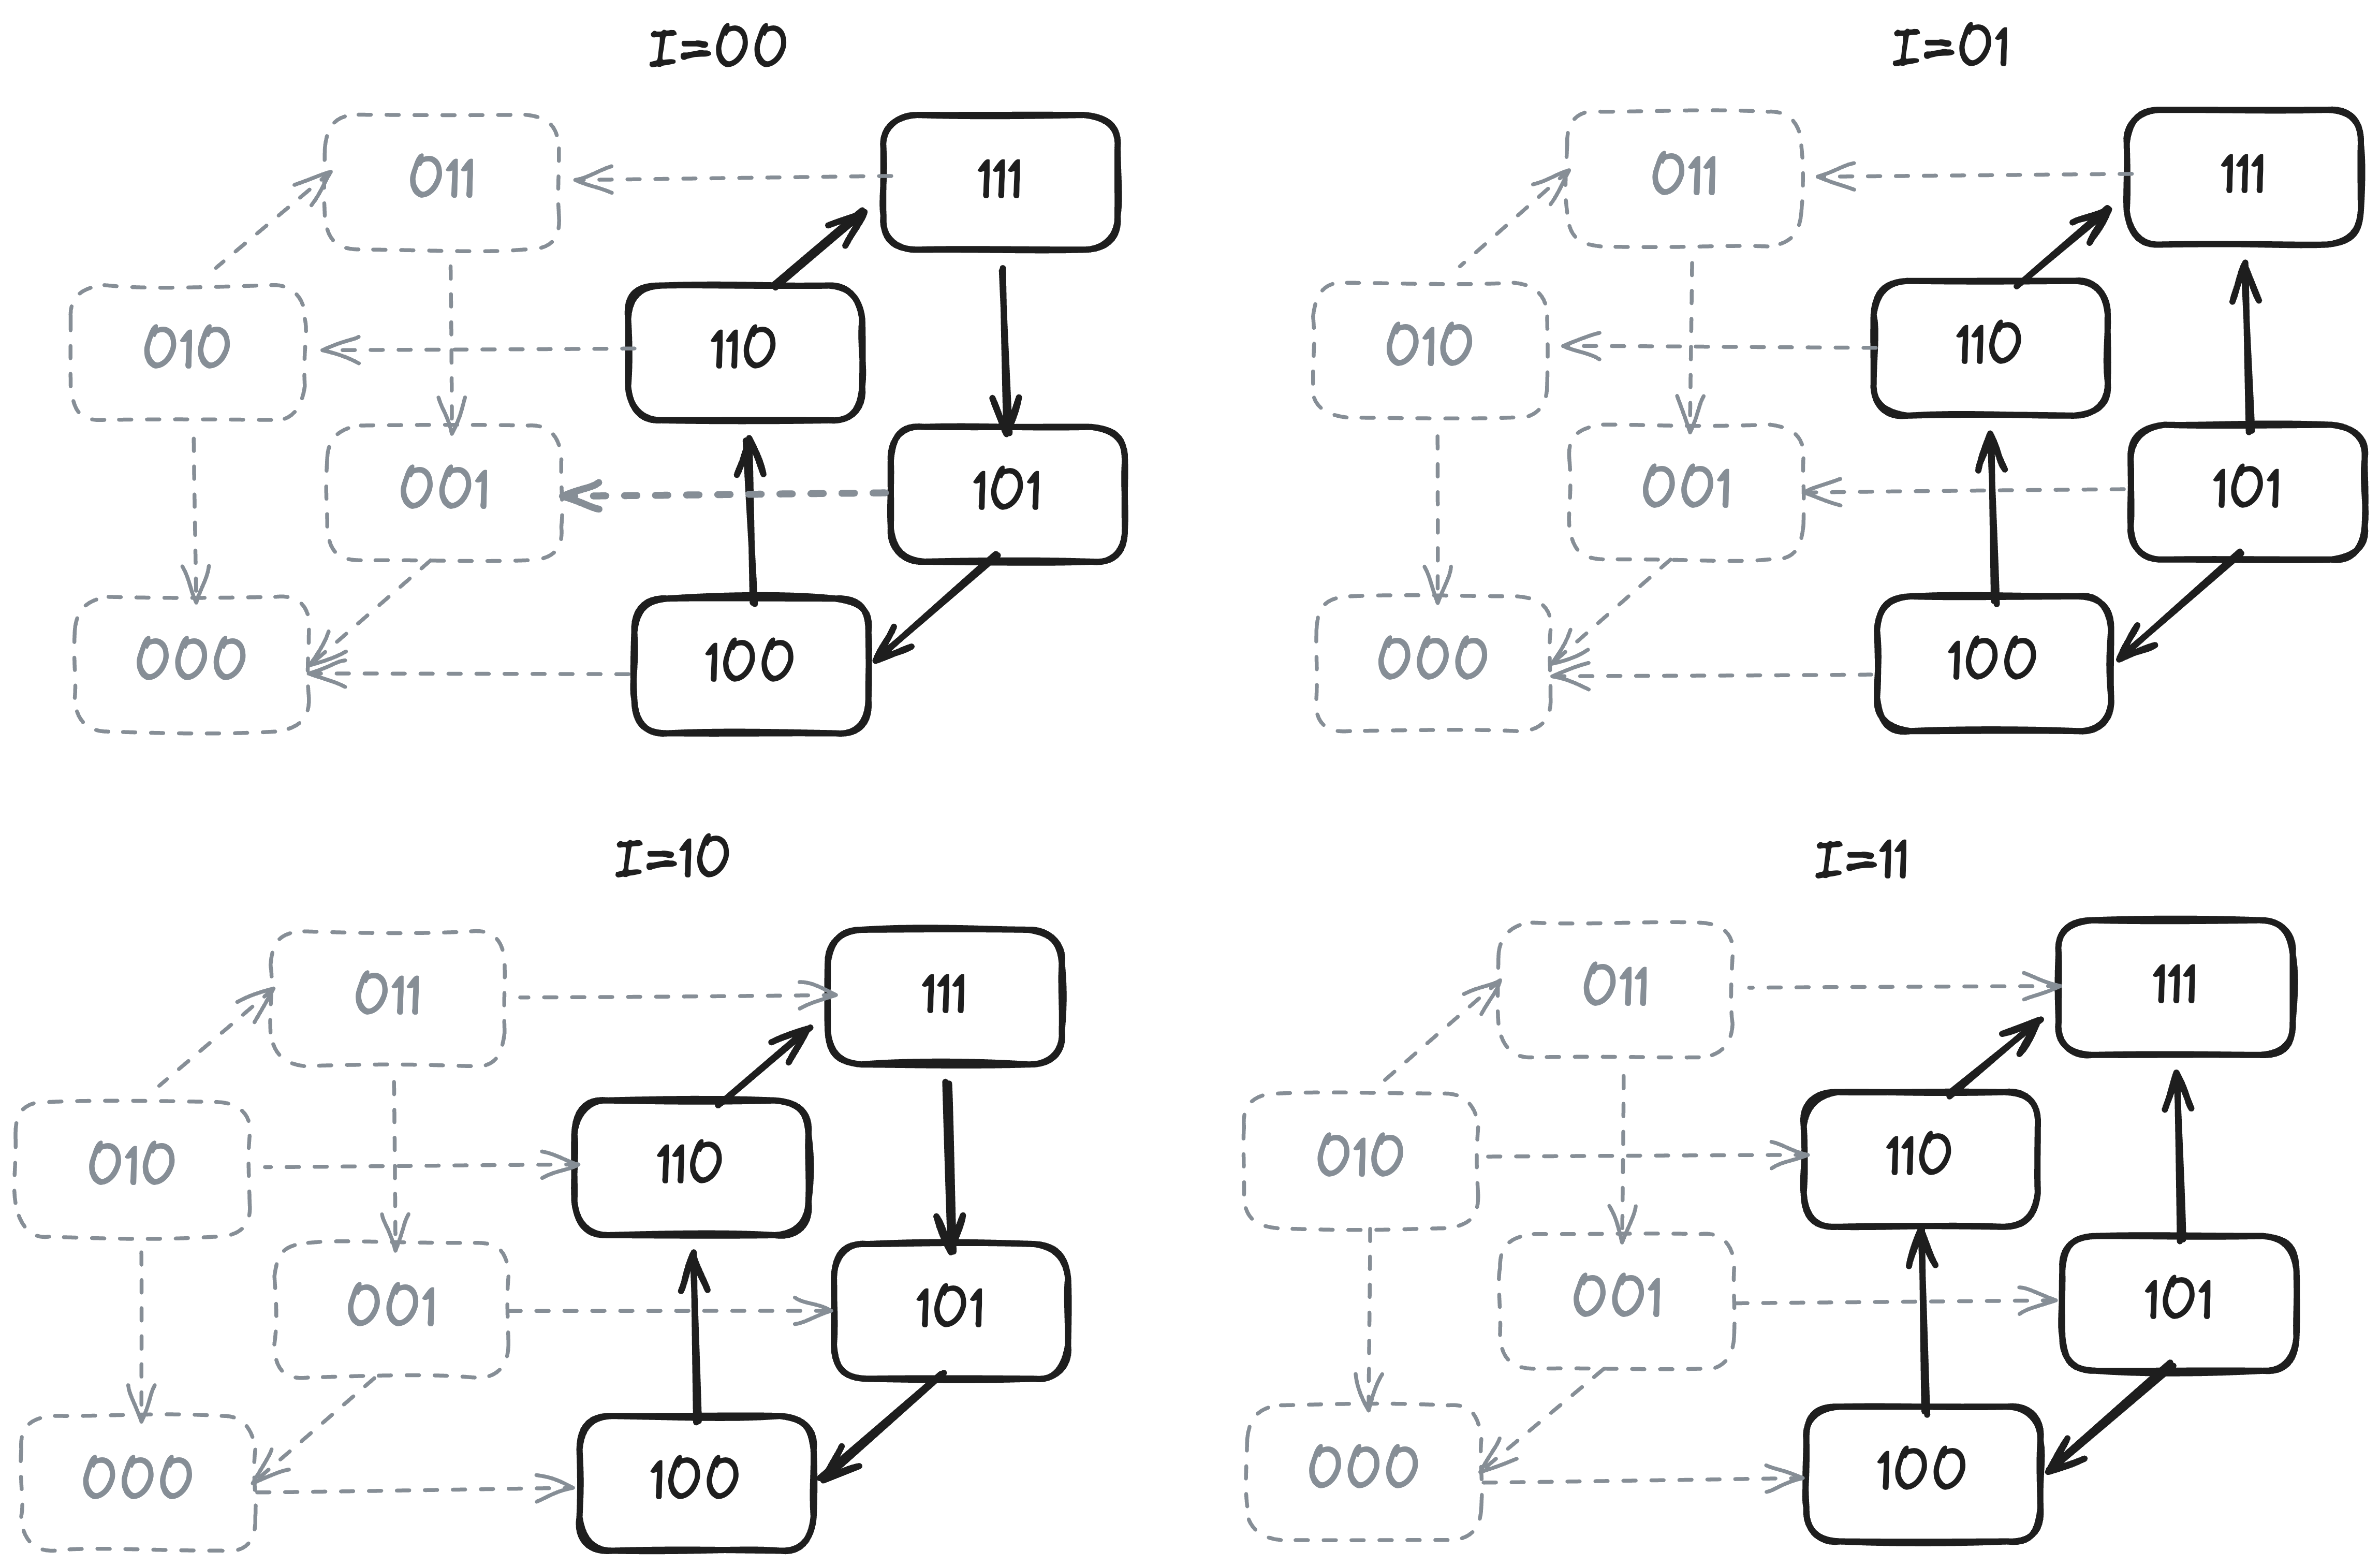
\includegraphics[width=0.8\textwidth]{Figures/psbn_perturbed_stg.png}
	\caption{\textbf{Perturbed STG of a PSBN.} An example of a PSBN with four interpretations perturbed with a perturbation x$1\unspecified\unspecified$.}
	\label{fig:psbn_perturbed_stg}
\end{figure}

\begin{definition}
    Let us assume an interpretation $\interpretation \in \allInterpretations$ of a \PBN{} $\widehat{\pbnMath} = \{\expr_1, \ldots, \expr_n\}$ with $m$ nullary function symbols $\allFunSymbols = \{\funSymbol_1, \ldots, \funSymbol_m \}$ where $\STG(\widehat{\pbnMath}(\interpretation)) = \vertices \times \edges$. Also, have a given source state $s \in \bools^n$, a perturbation $\perturbation \in \allPerturbations$, a and a time period $z \in \Nats_{\infty}$, after which the perturbation is withheld. \emph{A perturbed run $\run_{\perturbation}$} is a run which satisfies the following conditions:
    $$
    \run_{\perturbation}(t) = \begin{cases}
        s & \text{iff } t = 0 \\
        \pertApply(s, \perturbation) & \text{iff } t = 1 \\
        s'  \text{ s. t. } \run(t-1) = s'' \land (s'', s') \in \edges_{\perturbation} & \text{iff }  t'+z > t > t' + 1 \\
        s'  \text{ s. t. } \run(t-1) = s'' \land (s'', s') \in \edges & \text{iff } t > t'+z
    \end{cases}
    $$
    A set $\allRuns_{\perturbation}(\pbnMath(\interpretation), s, z)$ is a collection of all perturbed runs $\run_{\perturbation}$ for a given perturbation $\perturbation$, applied to a state $s$ with perturbation being withheld after $z$ time-steps.
\end{definition}

Notice, that again the definitions of perturbation and its application to a source state remain almost the same as in the \autoref{def:perturbed_run}. The only differences are that we now also consider the interpretation of the \PBN{} instance. Moreover, since this chapter focuses on source-target control, the perturbation is always applied just to a given source state.


\subsection{Control types and goal}
\label{ss:control_types_and_goal}

Finally, we can define the source-target control problem goal in the context of partially specified Boolean networks. Here, we consider three types of perturbations: one-step, permanent, and temporary perturbations. The definitions of these perturbation types are similar to those used in classical Boolean networks~\cite{Su2019CMSB,Su2020}, but adapted to the context of partially specified Boolean networks.

\begin{definition}
\label{def:psbn_control}
Assume having a \PBN{} $\pbnMath = \{\expr_1, \ldots, \expr_n\}$ with $m$ nullary function symbols $\allFunSymbols = \{\funSymbol_1, \ldots, \funSymbol_m \}$, an interpretation $\interpretation \in \allInterpretations$, a source state $s \in \bools^n$, and a target state $t \in \bools^n$ such that $t \in \bigcup \allAttractors(\pbnMath(\interpretation))$. Then, we say that a perturbation $\perturbation \in \allPerturbations$ \emph{controls} $\pbnMath(\interpretation)$ from $s$ to $t$ via:

\begin{itemize}
	\item \emph{One-step perturbation}: if for all $\run \in \allRuns_{\perturbation}(\pbnMath(\interpretation), s, 1)$, $t \in inf(\run)$. That is, after performing the perturbation for a single time-step ($\pertApply(s, \perturbation)$), $t$ is always visited infinitely often without further restricting the network in any way.
	\item \emph{Permanent perturbation}: if for all $\run_{\perturbation} \in \allRuns_{\perturbation}(\pbnMath(\interpretation), \perturbation(s), \infty)$, $t \in inf(\run_{\perturbation})$. That is, $t$ is always visited infinitely often assuming the perturbed variables remain constant to their perturbed value.
	\item \emph{Temporary perturbation}: if for all $\run_{\perturbation} \in \allRuns_{\perturbation}(\pbnMath(\interpretation), \perturbation(s), z+k)$, there exist such time period $z$ that for every $k \in \NatsZero$ we have $t \in inf(\run_{\perturbation})$. Intuitively, the system can evolve for an arbitrary number of time-steps while assuming the perturbed variables are constant. But there must exist some time period $z$ after which if the perturbation is withheld, run reaches (or remains in) $t$ infinitely often.
\end{itemize}

\end{definition}

Here, note several observations regarding the presented types of \PBN{} control. The one-step and permanent perturbations are rather straightforward since they either do not require any further adjustment of the network's transition system (one-step perturbation) or they require a simple restriction of the transition system to the subspace of states admissible by the perturbation (permanent perturbation). The temporary perturbation, however, is more complex since the network transition system needs to be adjusted only for a finite number of time-steps. The number of these time-steps is not know in advance or specific since the Boolean network is not considered to be observable. Typically, we assume, that network reaches some ``intermediate'' attractor within $\edges_{\perturbation}$ an in any of these states, the perturbation can be withheld. Oftentimes, this intermediate attractor contains the target state $t$ itself. In such case, the exact same perturbation works with both temporary and permanent applications.

Moreover, as already noted, the assumption that target state $t$ is a member of an attractor guarantees that if visited once in an unperturbed system, it is in fact visited infinitely often. Second, permanent control could force a particular $t$ to be visited infinitely often even though it is not a member of any attractor in the original $\pbnMath(\interpretation)$. This is because the perturbed variables remain fixed indefinitely, as opposed to one-step and temporary perturbations where the restrictions are eventually lifted. We allow for such case in the phenotype control as we see in the following (\autoref{chapter:phenotype_control_psbn}). Here, to maintain the comparability between all three perturbation types, we strictly restrict ourselves to the interpretations where target is an attractor state.  

Note that under this assumption, any successful permanent perturbation is also successful as a temporary perturbation, since the control can be released once target is reached. If we consider the cases where permanent control can introduce the target attractors, this property no longer holds. Nevertheless, a permanent perturbation can also potentially cause target to not be visited infinitely often by disturbing the attractor in which target resides, or it can cause the attractor to be unreachable within the perturbed state space. In this case, such permanent perturbation simply cannot control the network towards the desired target. An example of such scenario (target being unreachable due to permanent perturbation) is shown in \autoref{ex:only_temporary_working}. 

\begin{figure}
    \centering
    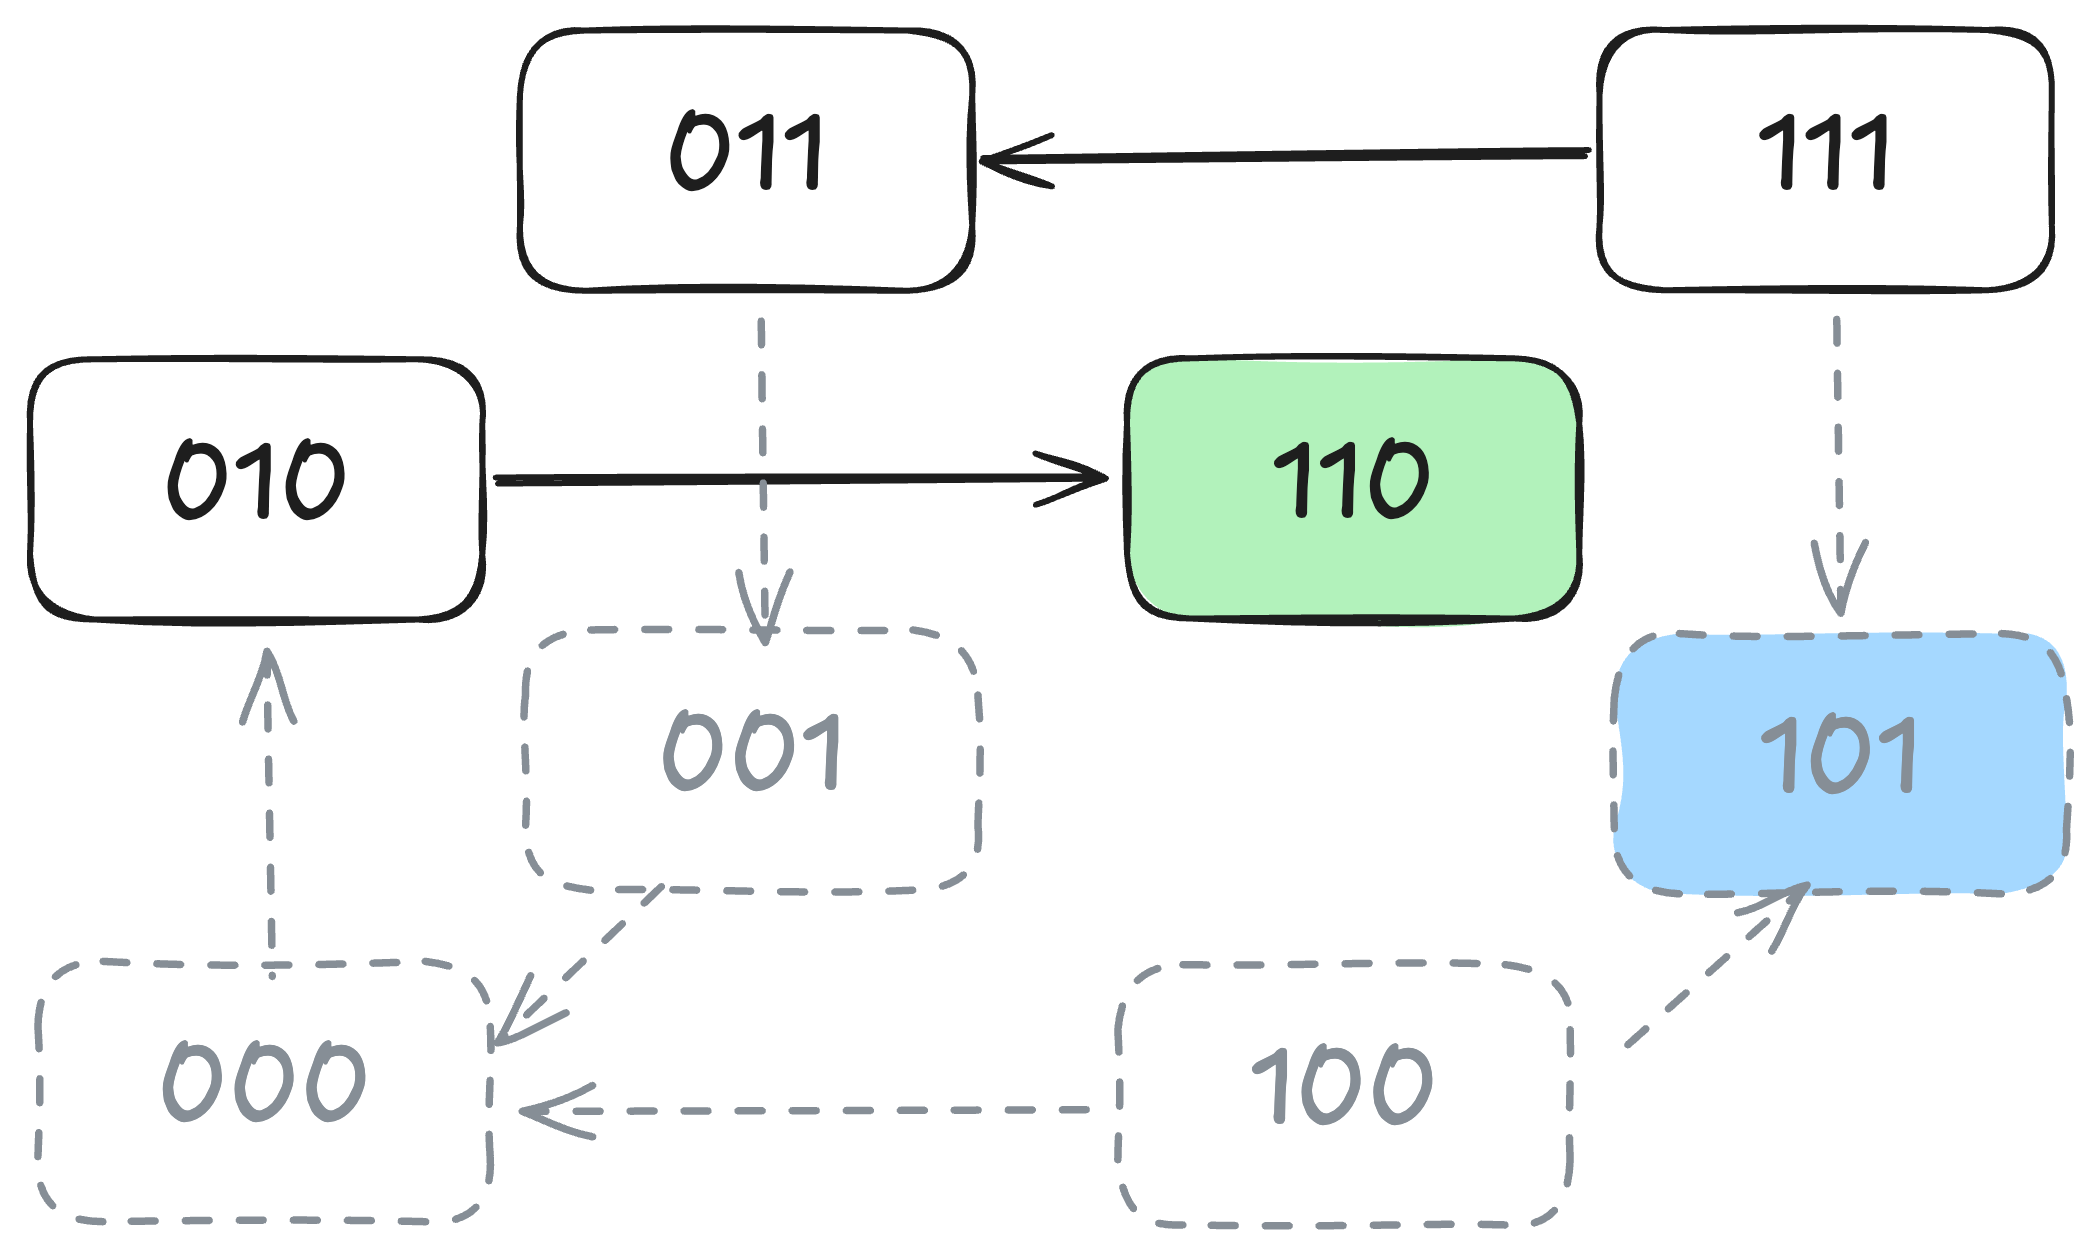
\includegraphics[width=0.45\textwidth]{Figures/only_temporary_working.png}
    \caption{\textbf{A specific case of a perturbed STG.} An example of an STG where a temporary perturbation control the network while one-step or permanent perturbations do not guarantee control.} 
    \label{fig:only_temporary_working}
\end{figure}

\begin{example}
Consider STG from \autoref{fig:only_temporary_working}, source $s = 101$ (blue) and target $t = 110$ (green) with a perturbation $\perturbation = {*}1{*}$. By applying the perturbation, the network transitions from $s=101$ to $\pertApply(s, \perturbation) = 111$. In the shown STG, only solid arrows are admissible while the perturbation is applied. The whole (unperturbed) STG then also admits the dashed arrows. As a result, under permanent perturbation, there is no way of reaching $110$ from $111$. Meanwhile, in the context of a temporary perturbation, $011$ corresponds to a state when the control would be released. Once $011$ is reached, lifting the perturbation guarantees that $target=110$ is eventually reached as well. Finally, note that $\perturbation = {*}1{*}$ is also unsuccessful as a one-step perturbation. This is because by immediately lifting the perturbation, $\pertApply(s, \perturbation) = 111$ can non-deterministically return to $s = 101$---reaching target $t$ is therefore possible, but not guaranteed.
\label{ex:only_temporary_working}
\end{example}

\subsection{Robustness}

In practice, our goal is to not only find perturbations that successfully control the network, but that are efficient and biologically feasible. Indeed, for a target state $t$ any naive perturbation $\perturbation = t$ successfully controls the network towards $t$, but is most likely not realistic. When the network is fully known, we typically focus on finding perturbations that are minimal in terms of size~\cite{Su2019CMSB,Su2020}. This search can be further restricted to network variables where the perturbation is known to be biologically feasible if such information is available.

However, if the network is not fully known, there are many possible interpretations, potentially resulting in very different sets of fair runs. In turn, most perturbations correctly control the network only for some subset of these interpretations. Since we do not know which interpretation (or interpretations) of the PSBN actually occurs in the wild, we may want to quantify such uncertainty. This allows us to search for perturbations that are not only small (in terms of perturbed variables), but that also work for a reasonable portion of the \PBN{} interpretations. Formally, this is captured by the metric of perturbation \emph{robustness}~\cite{Brim2021}:

\begin{definition}
	The \emph{robustness} $\robustness$ of a perturbation $\perturbation \in \bools_\unspecified^n$ for a \PBN{} $\pbnMath$ and a target state $t$ is defined as follows:
	\begin{align*}
		\robustness(\perturbation) = \frac{\mid \{ \interpretation \in \allInterpretations \mid \perturbation~\text{\upshape controls}~\pbnMath(\interpretation) \} \mid}{\mid \{ \interpretation \in \allInterpretations \mid t \in \bigcup \allAttractors(\pbnMath(\interpretation)) \} \mid}
	\end{align*}

	Depending on context, the term \emph{controls} refers to either one-step, permanent, or temporary perturbation as defined above.
\end{definition}

\subsection{Control problem}

As we can see, both size and robustness are critical factors when selecting viable perturbations for a \PBN{}. To facilitate the search for such perturbations and to compare different perturbations, we define control problem for \PBN{} as computation of the \emph{control relation} of all perturbations that successfully control the network from a given source to a given target:

\begin{definition}
\label{def:control_relation}
Given a \PBN{} $\pbnMath = \{\expr_1, \ldots, \expr_n\}$ with $m$ nullary function symbols $\allFunSymbols = \{\funSymbol_1, \ldots, \funSymbol_m \}$, a source state $s \in \bools^n$, and a target state $t \in \bools^n$ such that there exists an interpretation $\interpretation \in \allInterpretations$ for which $t \in \bigcup \allAttractors(\pbnMath(\interpretation))$, the goal of the \emph{source-target control problem} is to compute a \emph{control relation} $\controlRelation_{X}$ -- the set of all pairs $\controlRelation_{X} = \{ \perturbation, \interpretation \} \subseteq \bools_\unspecified^n \times \allInterpretations$ such that $\perturbation$ controls $\pbnMath(\mathcal{I}_c)$ from $s$ to $t$ assuming a type of perturbations $X \in \{ O, P, T \}$ as one-step ($\controlRelation_{O}$), permanent ($\controlRelation_{P}$), or temporary ($\controlRelation_{T}$) control.
\end{definition}

The robustness measure gives us the ability to compare the ``quality'' of a single perturbation. To also compare the ``quality'' of different control relations (or control approaches in general), we extend the notion of robustness to be measurable on a control relation. Specifically, we define \emph{maximal robustness} $\rho_{\max}(\controlRelation_{X})$ to be the maximal robustness achievable by a single perturbation from $\controlRelation_{X}$, and \emph{union robustness} $\rho_{\cup}(\controlRelation_{X})$ to be the collective robustness achievable by all available perturbations: 
\begin{align*}
	\rho_{\max}(\controlRelation_{X}) &= \max_{\perturbation \in \controlRelation_{X}} \rho(\perturbation) \\
	\rho_{\cup}(\controlRelation_{X}) &= \frac{ \mid \bigcup_{\interpretation \in \controlRelation_{X}}\ \interpretation \mid }{\mid \{ \interpretation \in \allInterpretations \mid t \in \bigcup \allAttractors(\pbnMath(\interpretation)) \} \mid}
\end{align*}

Intuitively, the maximal robustness $\rho_{\max}$ gives us the best case scenario that can be achieved using a single perturbation from $Q$. Meanwhile, union robustness $\rho_{\cup}$ is the measure of how well a system can be controlled \emph{overall}. In particular, if union robustness is less than one, there are PSBN interpretations that cannot be controlled by any perturbation in $\allPerturbations$. Both measures are thus worth exploring, as each represents a slightly different optimization goal: While a control relation $\controlRelation_{X}$ with high $\rho_{\max}$ is generally more likely to provide a practically viable control strategy, another control relation with a higher $\rho_{\cup}$ may achieve control even for cases that are not feasible by the former $\controlRelation_{X}$.

\subsection{Summary}

To summarize, in this section we defined the source-target control problem for partially specified Boolean networks. We defined three types of perturbations: one-step, permanent, and temporary perturbations. Then, we defined the goal of the source-target control problem as computation of the control relation containing all perturbations that successfully control the network from a given source to a given target. Finally, we introduced the robustness metric to quantify the uncertainty of a perturbation in terms of the portion of PSBN interpretations it can control.

\section{Semi-symbolic method for one-step control}
\label{sec:target_semisymbolic}

Now we describe our computational framework for solving the one-step state perturbation control of \PBN{}. We start by introducing our approach for finding strong basins in a \PBN{}. Then we explain the framework for exploring \PBN{} STG and for manipulation with \PBN{} interpretations. Next, a concise workflow for \PBN{} control that employs the proposed algorithms is demonstrated. Finally, we present an evaluation of the method on a collection of \PBN{} models. 

\subsection{Semi-symbolic labelled strong basin search}
\label{ss:semi_symbolic_sb}

The foundation of our method is based on binary decision diagram (BDD~\cite{Bryant86}) representation of interpretation sets of a \PBN{}. The decision variables of the BDD are the nullary function symbols of the network meaning that every path from the root to a leaf in such a BDD represent a set of interpretations of the \PBN{} while states are represented explicitly.

Common logical operations on such BDDs (and, or, negation, ...) then correspond to set operations (intersection, union, complement, ...).  Furthermore, static regulation constraints (activation, inhibition, observability) can be formalized using Boolean formulae over interpretations, and we can, therefore, create a BDD which enforces all constraints imposed by the regulatory network and represents the set of only relevant interpretations.

As described in~\autoref{ss:psbn_stg}, \PBN{} dynamics $\STG(\pbnMath{})$ are represented as an edge-labelled state-transition graph, where each transition $s \to t$ has an associated set of interpretations $\interpretationSet(s, t) \subseteq \allInterpretations$ represented as a BDD. A~\emph{labelled state set} is a mapping $\vertices \to 2^{\allInterpretations}$ assigning to each state a set of interpretations. Furthermore, we suppose that the state space is represented \emph{explicitly}, meaning that all operations on states are performed element-wise (typically in parallel).

We consider basic procedures over an STG of a PSBN. Given a source state $s$ and a viable interpretation set $\interpretationSet$ of a PSBN $\pbnMath$, procedures \pre and \post yield a set of labelled states reachable in one step backward/forward from $s$ under interpretations from $\interpretationSet$: 
\begin{align*}
\pre(s, \interpretationSet) = \{ t \mapsto \interpretationSet_t \mid \forall \interpretation \in \interpretationSet_t : \interpretation \in \interpretationSet \land s \to_{\interpretation} t \}\\
\post(s, \interpretationSet) =\{ t \mapsto \interpretationSet_t \mid \forall \interpretation \in \interpretationSet_t : \interpretation \in \interpretationSet \land t \to_{\interpretation} s \}
\end{align*}

These procedures can be then used (e.g. using a fixed-point computation) to compute a maximal labelled state set of \emph{all} forward/backward reachable states from the source state $s$. The set contains all reachable states $t$ where each $t$ is associated with a maximal set of interpretations $\interpretationSet_t$ for which $t$ is reachable from $s$:

\begin{align*}
\fwd(s, \interpretationSet) = \{ t \mapsto \interpretationSet_t \mid \forall \interpretation \in \interpretationSet_t : \interpretation \in \interpretationSet \land s \to^*_{\interpretation} t \}\\
\bwd(s, \interpretationSet) =\{ t \mapsto \interpretationSet_t \mid \forall \interpretation \in \interpretationSet_t : \interpretation \in \interpretationSet \land t \to^*_{\interpretation} s \}
\end{align*}

This representation (explicit state space and symbolic interpretations) allows computing the reachability procedures in parallel. For the underlying implementation, we worked with internal libraries of the tool Aeon~\cite{aeon} which provides most of the necessary functionality, including a convenient format for specifying \PBN{s} and parallel reachability procedures.

For control of \PBN{}, we first need to determine the relevant interpretations $\interpretationSet_A(t)$ for the target state $t$, where $t$ is a part of some attractor. This process is described in \autoref{algo:attractor-params}. The algorithm is following: we first compute all reachable states, but~only the one from which we can also reach back the target state itself are a part of a TSCC. Otherwise, it is possible to reach some other component of the system from the target state, and that contradicts the notion of attractor. In the partially specified setting, we obtain a mapping of states to interpretations in which it is not possible to return to the target again. Therefore, in all these interpretations the target state is not a part of any attractor, and so we discard them from the full parameter space $\allInterpretations$ to obtain $\interpretationSet_A(t)$. 

\begin{algorithm}[h]
	\SetKwInOut{Input}{Input}
	\SetKwInOut{Output}{Output}
	\Input{\PBN{} $\pbnMath{}$, target attractor state $\var{t}$}
	\Output{Attractor interpretations $\interpretationSet_A(\var{t})$}
	\BlankLine
	$\var{F} \gets \fwd(\var{t}, \allInterpretations)$\;
	$\var{B} \gets \bwd(\var{t}, \allInterpretations)$\;
	\tcc{For every state, compute the BDD difference}
	$\var{NA} \gets \var{F} \setminus \var{B}$\;
	\Return{$\allInterpretations \setminus \bigcup_{\var{s} \in \vertices(\pbnMath)}$ \var{NA}(\var{s})}\;
	\caption{Compute attractor interpretations $\interpretationSet_A(\var{t})$.}
	\label{algo:attractor-params}
\end{algorithm}


The key observation for controlling \PBN{s} is that an attractor is always reached from its strong basin (as explained in \autoref{def:basins}). From all other states, it is possible to reach also some other attractor; therefore, reaching the target attractor is not guaranteed. When the attractor's strong basin for all interpretations is known, we can compute the control mapping $\controlRelation_O$ from a source state to the target attractor by considering Hamming differences between the source and the states of the strong basin. 

Our algorithm is based on the fixed-point approach for strong basin computation in fully specified BNs~\cite{Paul2018CMSB}. The premise is that only states from which it is possible to reach the attractor (weak basin) can be part of the strong basin. The weak basin of the attractor is computed using standard reachability algorithms, for example, BFS. Then states are iteratively removed if it is possible to leave the basin from them (and therefore not reach the given attractor). Finally, if there are no states left to remove, the fixed-point is achieved, and the strong basin is found.


\begin{algorithm}[h]
	\SetKwInOut{Input}{Input}
	\SetKwInOut{Output}{Output}
	\Input{PBN $\pbnMath$, target state $\var{t}$, interpretations $\interpretationSet_A(\var{t})$}
	\Output{labelled state set $\vertices \to
		2^{\interpretationSet_A(\var{t})}$ representing the strong basin}
	\BlankLine
	$\var{SB} \leftarrow \bwd(\var{t}, Ap(\var{t}))$\;
	$\var{to\_update} \leftarrow \var{s}$ in $\{ \var{s} \in \vertices \mid \var{SB}(\var{s}) \not= \emptyset \}$\;
	\Do{$\var{to\_update} \neq \emptyset$}{
		$\var{updated} \gets \emptyset$\;
		$\var{to\_remove} \gets \forall \var{s} \in \vertices \rightarrow \emptyset$\;
		\textbf{parallel} \For{$\var{s}$ in $\var{to\_update}$}{  
			\For {$\var{t}$ in $\post(\var{s})$} {
				\tcc{Recompute interpretations leading outside of basin}
				$\var{to\_remove}(\var{s}) \gets \var{SB}(\var{s}) \cap \interpretationSet(\var{s}, \var{t}) \cap (\interpretationSet_A(\var{t}) \setminus \var{SB}(\var{t}))$\;
			}
			\uIf{$\var{to\_remove}(\var{s}) \neq \emptyset$} {
				$\var{updated} \gets \var{updated} \cup \{s\}$ \;
			}
		}
		$\var{to\_update} \gets \emptyset$\;
		\For {$\var{s}$ in $\var{updated}$} {
			\tcc{Update strong basin}
			$\var{SB}(\var{s}) \gets \var{SB}(\var{s}) \setminus \var{to\_remove}(\var{s})$\;
			\tcc{Only predecessors of updated vars might be updated in the next iteration}
			$\var{to\_update} \leftarrow \var{updated} \cup \pre(\var{s})$ \;
		}
	}
	\Return{\var{SB}}\;
	\caption{Parallel strong basin computation.}
	\label{algo:strong-basin}
\end{algorithm} 

In \autoref{algo:strong-basin}, we extend the approach from~\cite{Paul2018CMSB} onto \PBN{}. For each state we remember under which interpretations it is in the basin, starting with the labelled weak basin (backward reachability from the target state). Then we iterate over the basin's states. For~each state, we consider its successors, and we compute the interpretations for which some successor is \emph{not in the strong basin}. In these interpretations, it is possible to leave the basin, and therefore these interpretations are not part of the strong basin and so we remove them for this state. 

We can process the states in parallel and compute for them the interpretations which are not part of the strong basin. To avoid writing to the strong basin structure while it is intensively read from, we store the interpretations which should be removed separately, and after it is computed, we update the strong basin structure sequentially. The procedure is repeated until nothing more can be removed from the strong~basin.

\subsection{Control computation workflow}

Now we can describe a complete workflow for computing the source-target control in \PBN{s}, depicted in \autoref{fig:workflow}. The~workflow consists of three inputs and three computation steps, resulting in the control mapping $\controlRelation_O$. 

Given an input \PBN{} and a target attractor state $t$, we start by computing valid interpretation set $\interpretationSet_A(t)$ using \autoref{algo:attractor-params}. Then, the labelled strong basin is computed from the \PBN{} with target attractor state $t$ and its valid interpretations $\interpretationSet_A(t)$ using \autoref{algo:strong-basin}. After that, from the strong basin and the source state, we obtain the complete control mapping. Notice that we do not need to know the source state for computing the strong basin and that we can re-use the target's strong basin for obtaining control for different~sources.

To compute the control mapping, observe that viable controls correspond exactly to the Hamming differences (the variables with opposite values) between the source state and the states of the strong basin; yielding one viable perturbation $\perturbation$ for every state $s$ in the strong basin $\var{SB}$. Any other control $\perturbation'$ does not reach the strong basin and therefore does not guarantee to reach the target attractor (for these, $\controlRelation_O(\perturbation) = \emptyset$). A perturbation $\perturbation$ is then viable only for interpretations for which $s$ appears in the strong basin, we thus set $\controlRelation_O(\perturbation) = \var{SB}(s)$. 

\begin{figure}
\checkoddpage
\edef\side{\ifoddpage l\else r\fi}
\makebox[\textwidth][\side]{% 
	\begin{minipage}{\fullwidth}
	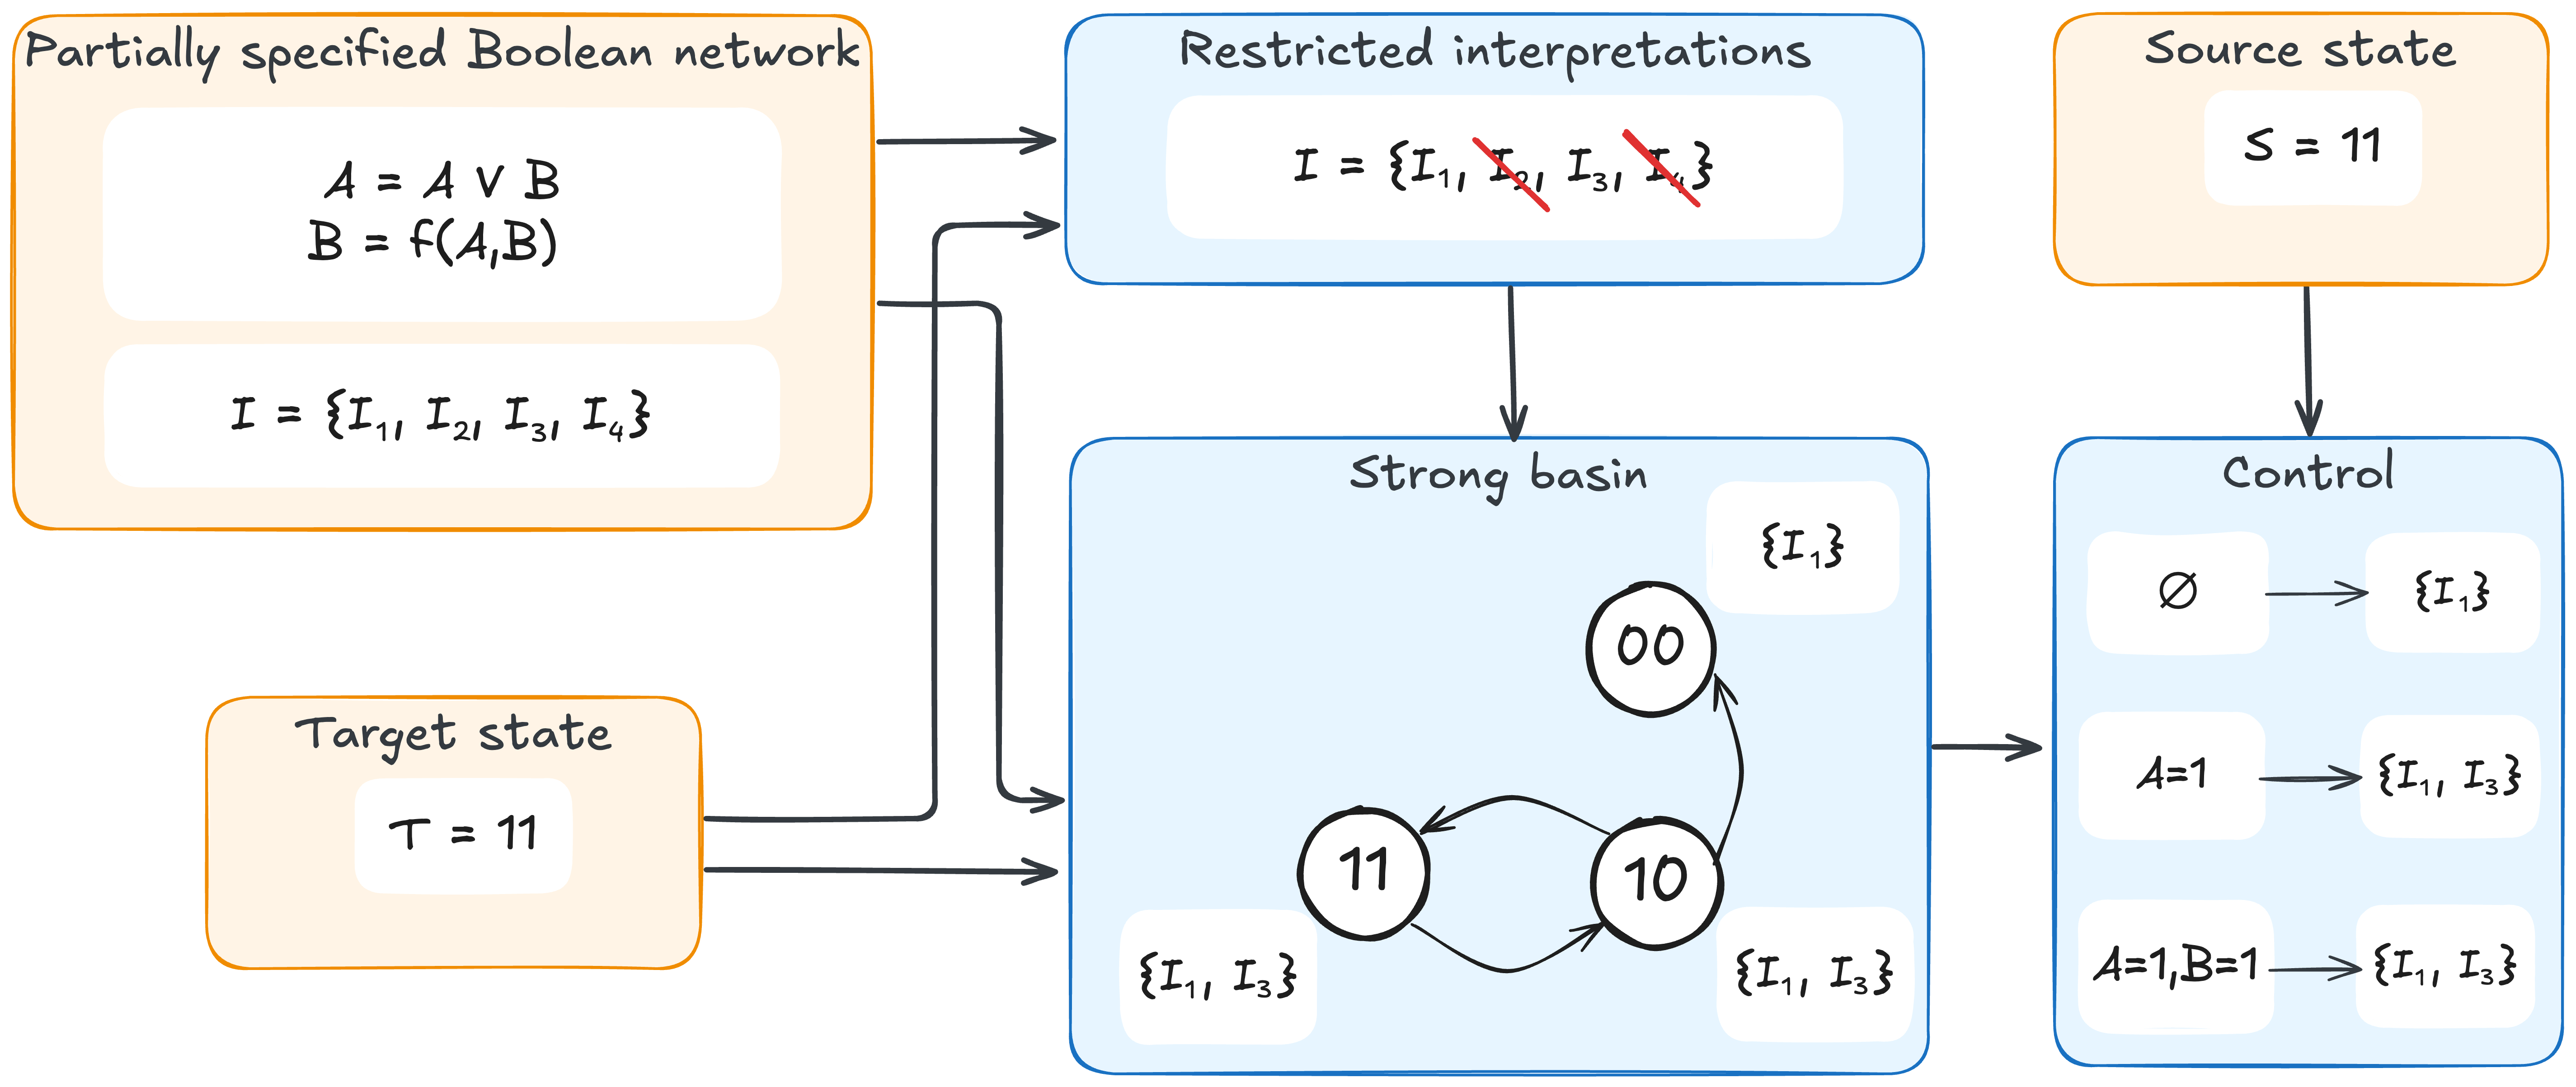
\includegraphics[width=\textwidth]{Figures/workflow.png}
	\caption{
		\textbf{Workflow of computing the source-target control problem.} Parts in the orange boxes represent inputs and blue boxes represent (intermediate) results.
	}
	\label{fig:workflow}
\end{minipage}%
}%
\end{figure}

% Is the 2nd subfigure (Restricted parametrisation Ap) correct?
% Authors: Yes.


Finally, we can compute the size and robustness of each control as we have all knowledge regarding the variables which need to be controlled and interpretations for which the controls work. If it is desired, we can construct a \emph{witness} \PBN{} instance for a perturbation $\perturbation$ (a fully specified BN where the given control works) by fixing the parameters from $\controlRelation_O(\perturbation)$.

In complex and highly unspecified models, it is not unusual for empty perturbation $\emptyset$ to control the network where in some interpretations and therefore no action would be needed to control the model. This is because, in some interpretations, the source might already be a part of the target's strong basin. If this case is considered unrealistic (since there is probably a need for control, thus these interpretations appear to be invalid), the interpretations $\interpretationSet_A(t)$ can be replaced with a custom set of~interpretations.

The resulting set of all available controls can be then used for e.g., cell reprogramming. However, we might obtain many possible controls, and we need to decide which one should be applied. To do that, we can decide based on the size of control or its robustness. The control set can be arbitrarily filtered discarding controls with size bigger than the trivial control (which always has 100\% robustness) or bigger than some set size. Similarly, the control relation can be pruned based on too low robustness. It is left to the actual application to decide which control would best suit its needs. Namely, whether it is more important for the control set to be small or to be robust, as typically, there is rarely available perturbation which would be optimal in both these factors.

% \enlargethispage*{5mm}
\subsection{Results}

\label{sec:results}
We evaluate our approach on two real-life BN models. We compare the performance of our approach using a different number of parameters implanted into the models, resulting in different size of relevant parameter space. We conducted all measurements using a machine equipped with AMD Ryzen Threadripper 2990 WX 32-Core Processor and 64 GB of~memory.

The first model is a \emph{cell-fate decision model}~\cite{Calzone2010}. The model provides a high-level view of possible different cell fates such as pro-survival, necrosis or apoptosis. We used an adapted version of this model, where only regulatory network is provided and all the functions are left unspecified. Then, we selected seven biologically relevant attractors and computed strong basins only for these attractors in several model instances differing in the number of unknown parameters (see \autoref{table:results}).

The second model, a \emph{myeloid differentiation network}~\cite{Krumsiek2011}, was designed to model a bone marrow tissue cell differentiation from common myeloid cell to specialised blood cells (megakaryocytes, erythrocytes, granulocytes, and monocytes). The original network has eleven nodes and six attractors. We derived several partially specified versions of the model by arbitrarily substituting update functions of the model for function symbols. Similarly to the previous case, we used only attractors of the original network when computing strong basins for partially specified versions of the model. 
%For both models, we computed the basins of the mentioned attractors. 
The results are again shown in \autoref{table:results}.

% % %\enlargethispage*{5mm}
% % \begin{specialtable}[H]
% %   \tablesize{\small}
	
% % 	%\setlength{\tabcolsep}{0.3em} % for the horizontal padding
% % 	%\renewcommand{\arraystretch}{1.1}% for the vertical padding
% % 	\setlength{\cellWidtha}{\columnwidth/6-2\tabcolsep-0.0in}
% % \setlength{\cellWidthb}{\columnwidth/6-2\tabcolsep-0.0in}
% % \setlength{\cellWidthc}{\columnwidth/6-2\tabcolsep+0.0in}
% % 	\setlength{\cellWidtha}{\columnwidth/6-2\tabcolsep+0.0in}
% % \setlength{\cellWidthb}{\columnwidth/6-2\tabcolsep+0.0in}
% % \setlength{\cellWidthc}{\columnwidth/6-2\tabcolsep+0.0in}
% % \scalebox{1}[1]{\begin{tabularx}{\columnwidth}{>{\PreserveBackslash\centering}m{\cellWidtha}>{\PreserveBackslash\centering}m{\cellWidthb}>{\PreserveBackslash\centering}m{\cellWidthc}>{\PreserveBackslash\centering}m{\cellWidtha}>{\PreserveBackslash\centering}m{\cellWidthb}>{\PreserveBackslash\centering}m{\cellWidthc}}
\begin{table}
	\footnotesize
	\caption{Results of strong basin computation. The values are stated as ranges because we computed strong basins of all attractors considered in the given models. The second column shows the number of model's parameters. The third column shows count ranges of interpretations which contain the given attractor. The fourth and fifth columns display ranges of the number of states in the weak (resp. strong) basins. The last column contains ranges of times needed to compute strong basins.}
	\label{table:results}
	\setlength{\tabcolsep}{4pt}
	\begin{tabular}{llllll}
		\toprule
		\textbf{Model} &  \boldmath$\mid \allFunSymbols \mid$  & \boldmath$\mid \interpretationSet_A(t) \mid$ & \textbf{\# WB States} & \textbf{\# SB States} & \textbf{Time} \\
		\midrule
		\multirow{3}{*}{Cell-Fate}  & 1 & 1 & 258,000--491,184 & 32--352 & 4.4--9.19 s \\ 
		& 8 & 1--4 & 258,000--491,464 & 21--79 & 4.63--13.42 s \\ 
		& 20 & 7--56 & 258,048--491,520 & 1632--262,144 & 5.82--26.59 s \\ 
		\midrule
		\multirow{4}{*}{Myeloid}   & 1 & 1 & 128--1152 & 64--384 & 8--30 ms \\ 
		& 32 & 63--2052 & 224--1984 & 64--1472 & 14--214 ms \\ 
		& 70 & \num{5.9e4}--\num{1.8e7} & 1512--2048 & 256--2048 & 147--1717 ms \\ 
		& 94 & \num{3.4e6}--\num{3.7e9} & 2008--2048 & 1024--2048 & 0.6--15.38 s \\ 
		\bottomrule
	\end{tabular}
\end{table}
% \end{tabularx}}
% \end{specialtable}

Next, we ``virtually'' compare our approach to a na\"ive approach based on an interpretation enumeration (i.e., computing results for each interpretation separately). In~\cite{Baudin2019}, a strong basin of (fully specified) asynchronous BNs is computed using a block decomposition method with 4 ms needed to finish the computation for the \emph{myeloid model}. Even if the reported hardware was slower than in our case, and we assume that the strong basin computation for one interpretation would last only 1 ms, the fully unspecified myeloid model contains an attractor which is present in \num{3.7e9} interpretations. Therefore, the expected time for computing a strong basin for all interpretations with 32-fold parallelization is more than a day compared to less than 27 s achieved using our semi-symbolic approach.

We evaluate the scalability of our approach on a fully unspecified myeloid model. The results are shown in \autoref{table:scalability}. The computation was restricted to the specified amount of CPUs. The final speed-up achieved on our machine, when using 32 CPUs compared to a non-parallel CPU usage was about 10-fold.

% %\enlargethispage*{5mm}
% \begin{specialtable}[H]
%  \tablesize{\small}
\begin{table}
	\caption{\textbf{Scalability of strong basin computation.} The strong basins are computed on attractors of myeloid model~\cite{Krumsiek2011}.}
	\setlength\tabcolsep{0pt}
	\begin{tabular*}{\linewidth}{@{\extracolsep{\fill}}lcccccc}
		\hline
		\textbf{CPUs} &  $\mathbf{\attractor_1}$  & $\mathbf{\attractor_2}$ & $\mathbf{\attractor_3}$ & $\mathbf{\attractor_4}$ & $\mathbf{\attractor_5}$ & $\mathbf{\attractor_6}$ \\
		\hline
		1 & 6.13 s & 99.31 s & 71.32 s & 130.17 s & 45.84 s & 136.65 s \\
		
		2 & 3.34 s & 54.32 s & 38.87 s & 71.31 s & 24.95 s & 74.29 s \\
		
		4 & 1.86 s & 31.3 s & 21.83 s & 40.31 s & 13.71 s & 42.26 s \\
		
		8 & 1.11 s & 19.34 s & 13.31 s & 24.68 s & 8.4 s & 26.49 s \\
		
		16 & 0.87 s & 14.03 s & 9.32 s & 17.56 s & 5.77 s & 18.86 s \\
		
		32 & 0.6 s & 10.98 s & 6.87 s & 13.22 s & 4.54 s & 15.38 s \\
		\bottomrule
	\end{tabular*}
	\label{table:scalability}
\end{table}

Now let us have a look at an example of how the results might be interpreted and a suitable control selected. Suppose that we want to reprogram an erythrocyte cell (attractor having factors \var{EKLF}=1 and \var{GATA-2}=0) into a monocyte cell (attractor having factors \var{cJun}=1 and \var{EgrNab}=1) of the myeloid model. First, we obtain a strong basin of the monocyte attractor having 1472 states yielding us 1472 possible control sets. We can observe that trivial, i.e., the most robust control strategy (setting variables so that we reach the attractor right after applying the control), has size 8. We can discard all controls with size 8 and larger as they are less optimal in all aspects than the trivial control. In our case, there are 1259 controls with a smaller size than the trivial one. 

Resulting smallest control sets have the size 1. However, the~best robustness among these controls is 46\%. Therefore, it is quite likely that it will not work in practice. If we allow the control to have size 2, we can use the control with 76.8\% robustness. Increasing the size further provides control with the size 3 and the robustness 92\% and so is highly likely to reprogram the cell's phenotype. 

To achieve only slightly more robustness (93.8\%), we may use a control of size 5. In this highly unspecified model, there is no control with 100\% robustness being smaller than the trivial one. It is not a rule of the thumb that with bigger size of control we obtain better robustness, for example, the control with the size 11 (the only one, with all variables, reversed compared to the original one) has the robustness of only 50\%. 

It can be seen that the unknown properties of \PBN{} make selection of one particular ``best`` control complicated. The smallest control has low chance to work in reality and while control of size 3 works has significantly better chance to work, the success of the control is not guaranteed and might be difficult to implement. This is why a careful in vitro experimentation is needed to verify the correctness of the control in reality. Nonetheless, the obtained control set still can help and highly reduce the exponential number of potential transcription factor combinations that could be theoretically tested in vitro.

\subsection{Summary}
In this section, we presented a semi-symbolic method for computing the source-target control of \PBN{} using one-step perturbations. The method is based on a fixed-point computation of the labelled strong basin of the target attractor. We demonstrated that our method is capable of controlling highly unspecified models in seconds, and is considerably faster than the na\"ive interpretation scan approach.
%\enlargethispage*{6mm}
% \textcolor{red}{We introduced the control problem for partially specified Boolean networks and we proposed an algorithm for solving the source-target variant of this problem using one-step perturbations. The core procedure of the algorithm is a fixed-point computation of the labelled strong basin of the given target. The method we proposed is semi-symbolic --- it relies on a unique integration of symbolic (based on BDD representation) and explicit (based on enumerative model checking) formal methods. We demonstrated  that our approach is capable if controlling highly unspecified models in seconds. Owing to the doubly exponential explosion of the number of possible parametrisations, such a result cannot be achieved with the na\"ive interpretation scan approach.}

\section{Symbolic method for one-step, temporary and permanent control}
\label{sec:ostp_symbolic}

In the previous section, we presented a method for computing the source-target control of \PBN{} using one-step perturbations. We have seen, that control size for one-step perturbations could be improved. To address this issue, we can consider more general types of perturbations, such as permanent or temporary perturbations. Moreover, in the meantime, the tool AEON was advanced to support symbolic representation of states as well~\cite{benevs2022bdd}, which allows us to explore the whole perturbation space in parallel. Therefore, we can now propose a fully symbolic method for computing the source-target control of \PBN{} using one-step, temporary, and permanent perturbations.

% Real-world partially specified Boolean networks can have a large number of parameters and variables (and consequently, many admissible perturbations). It is not possible to explore the STGs of such networks explicitly. We propose novel symbolic algorithms to address this issue for the problem of BN control. These algorithms are based on the existing approaches for control of fully specified BNs. However, the addition of function symbols introduces extra complexity which we need to address. 

% On the one hand, identifying a single minimal perturbation that is successful for \emph{some} interpretation of the PSBN is not sufficient, as the robustness of such a perturbation can be very low, making it unlikely to work in practice. On the other hand, requiring that the perturbation is effective for \emph{all} possible interpretations may result in unnecessarily large perturbations. To provide a reasonably reliable method, we need to consider a large set of perturbations. Consequently, for performance reasons, our algorithms cannot test only a single perturbation at a time, but need to explore the whole perturbation space symbolically.

\subsection{Symbolic computation model}

Similarly to the previous method, we employ symbolic representation using binary decision diagrams (BDDs)~\cite{Bryant86}. However, in this case, we extend the use of BDDs to represent not just interpretation space symbolically, but also the sets of states. The main advantage of BDDs is that a logical operation (e.g. a conjunction) can be performed directly on two operand graphs, maintaining the compact representation throughout the whole computation. Due to this correspondence, we do not differentiate between a BDD and the Boolean function that it represents. Furthermore, note that any set or relation $X$ consisting of Boolean vectors (e.g. $X \subseteq \bools^k$) can be represented by a Boolean function that returns $1$ exactly for the members of $X$ and $0$ otherwise. Therefore, any such $X$ can be also represented using a BDD. In particular, this includes subsets of network states ($X \subseteq \bools^n$), subsets of PSBN interpretations ($X \subseteq \bools^m$), and relations of the two ($X \subseteq \bools^n \times \bools^m$). Logical operations on BDDs then correspond to set operations (e.g. $\cap \equiv \land$, $\cup \equiv \lor$, etc.).

Another important aspect is that a perturbation $\perturbation$ is not a Boolean vector, but rather a vector over $\bools_\unspecified$. Fortunately, in our algorithms, we do not need to manipulate whole perturbations. Instead, we only encode which variables in the network are perturbed ($q_i = 0$ or $q_i = 1$) and which are free ($q_i = \unspecified$). For this task, subsets of $\bools^n$ are sufficient. To summarize, we use the following notation:
\begin{itemize}
	\item $\vertices \equiv \bools^n$ encodes network states (vertices of $\STG(\pbnMath)$);
	\item $\allInterpretations \equiv \bools^m$ encodes network interpretations (i.e. the set of all possible function symbols valuations);
	\item $\mathbb{L} \equiv \bools^n$ encodes sets of perturbed variables (without the actual perturbation value).
\end{itemize}

Similar to the previous method, target state $t$ may not be an attractor state in all interpretations of the given PSBN. Consequently, instead of $\allInterpretations$, we again consider a smaller subset of interpretations $\interpretationSet_A \subseteq \allInterpretations$ where $t$ is guaranteed to be a member of some attractor. As this requires no functional changes to the presented algorithms, we generally use the set $\interpretationSet_A$, with the implicit assumption that a smaller $\interpretationSet'$ can be also used when desired.

The reason why we do not have to encode full perturbations is because in our algorithms, we use a relation $X \subseteq \vertices \times \allInterpretations \times \mathbb{L}$ to encode the full state of the system. In such an $X$, we assume that if the network is perturbed, only the states that are compatible with the perturbation are permitted within $X$ (this invariant is maintained throughout the algorithms). Consequently, in a triple $(v, 
\interpretation, l) \in X$ where $l_i$ encodes whether a variable is perturbed, $v_i$ encodes either the state of the network (when $l_i = 0$, i.e. unperturbed) or the constant value of the perturbation (when $l_i = 1$, i.e. perturbed).

We then use $\mathbb{X} = \vertices \times \allInterpretations \times \mathbb{L}$ as a shorthand for this extended set of perturbable states and network interpretations. We also write that a pair $(v, l) \in \vertices \times L$ is \emph{equivalent} to a perturbation $\perturbation \in \bools_\unspecified^n$, $(v, l) \equiv \perturbation$, if $\perturbation_i = \unspecified$ when $l_i = 0$, and $\perturbation_i = v_i$ when $l_i = 1$.
% Therefore, to decode full perturbation from the resulting relation $X \subseteq V \times C \times L$, the pairs of $V \times L$ must be considered. 

\begin{figure}[htp]
	\begin{centering}
		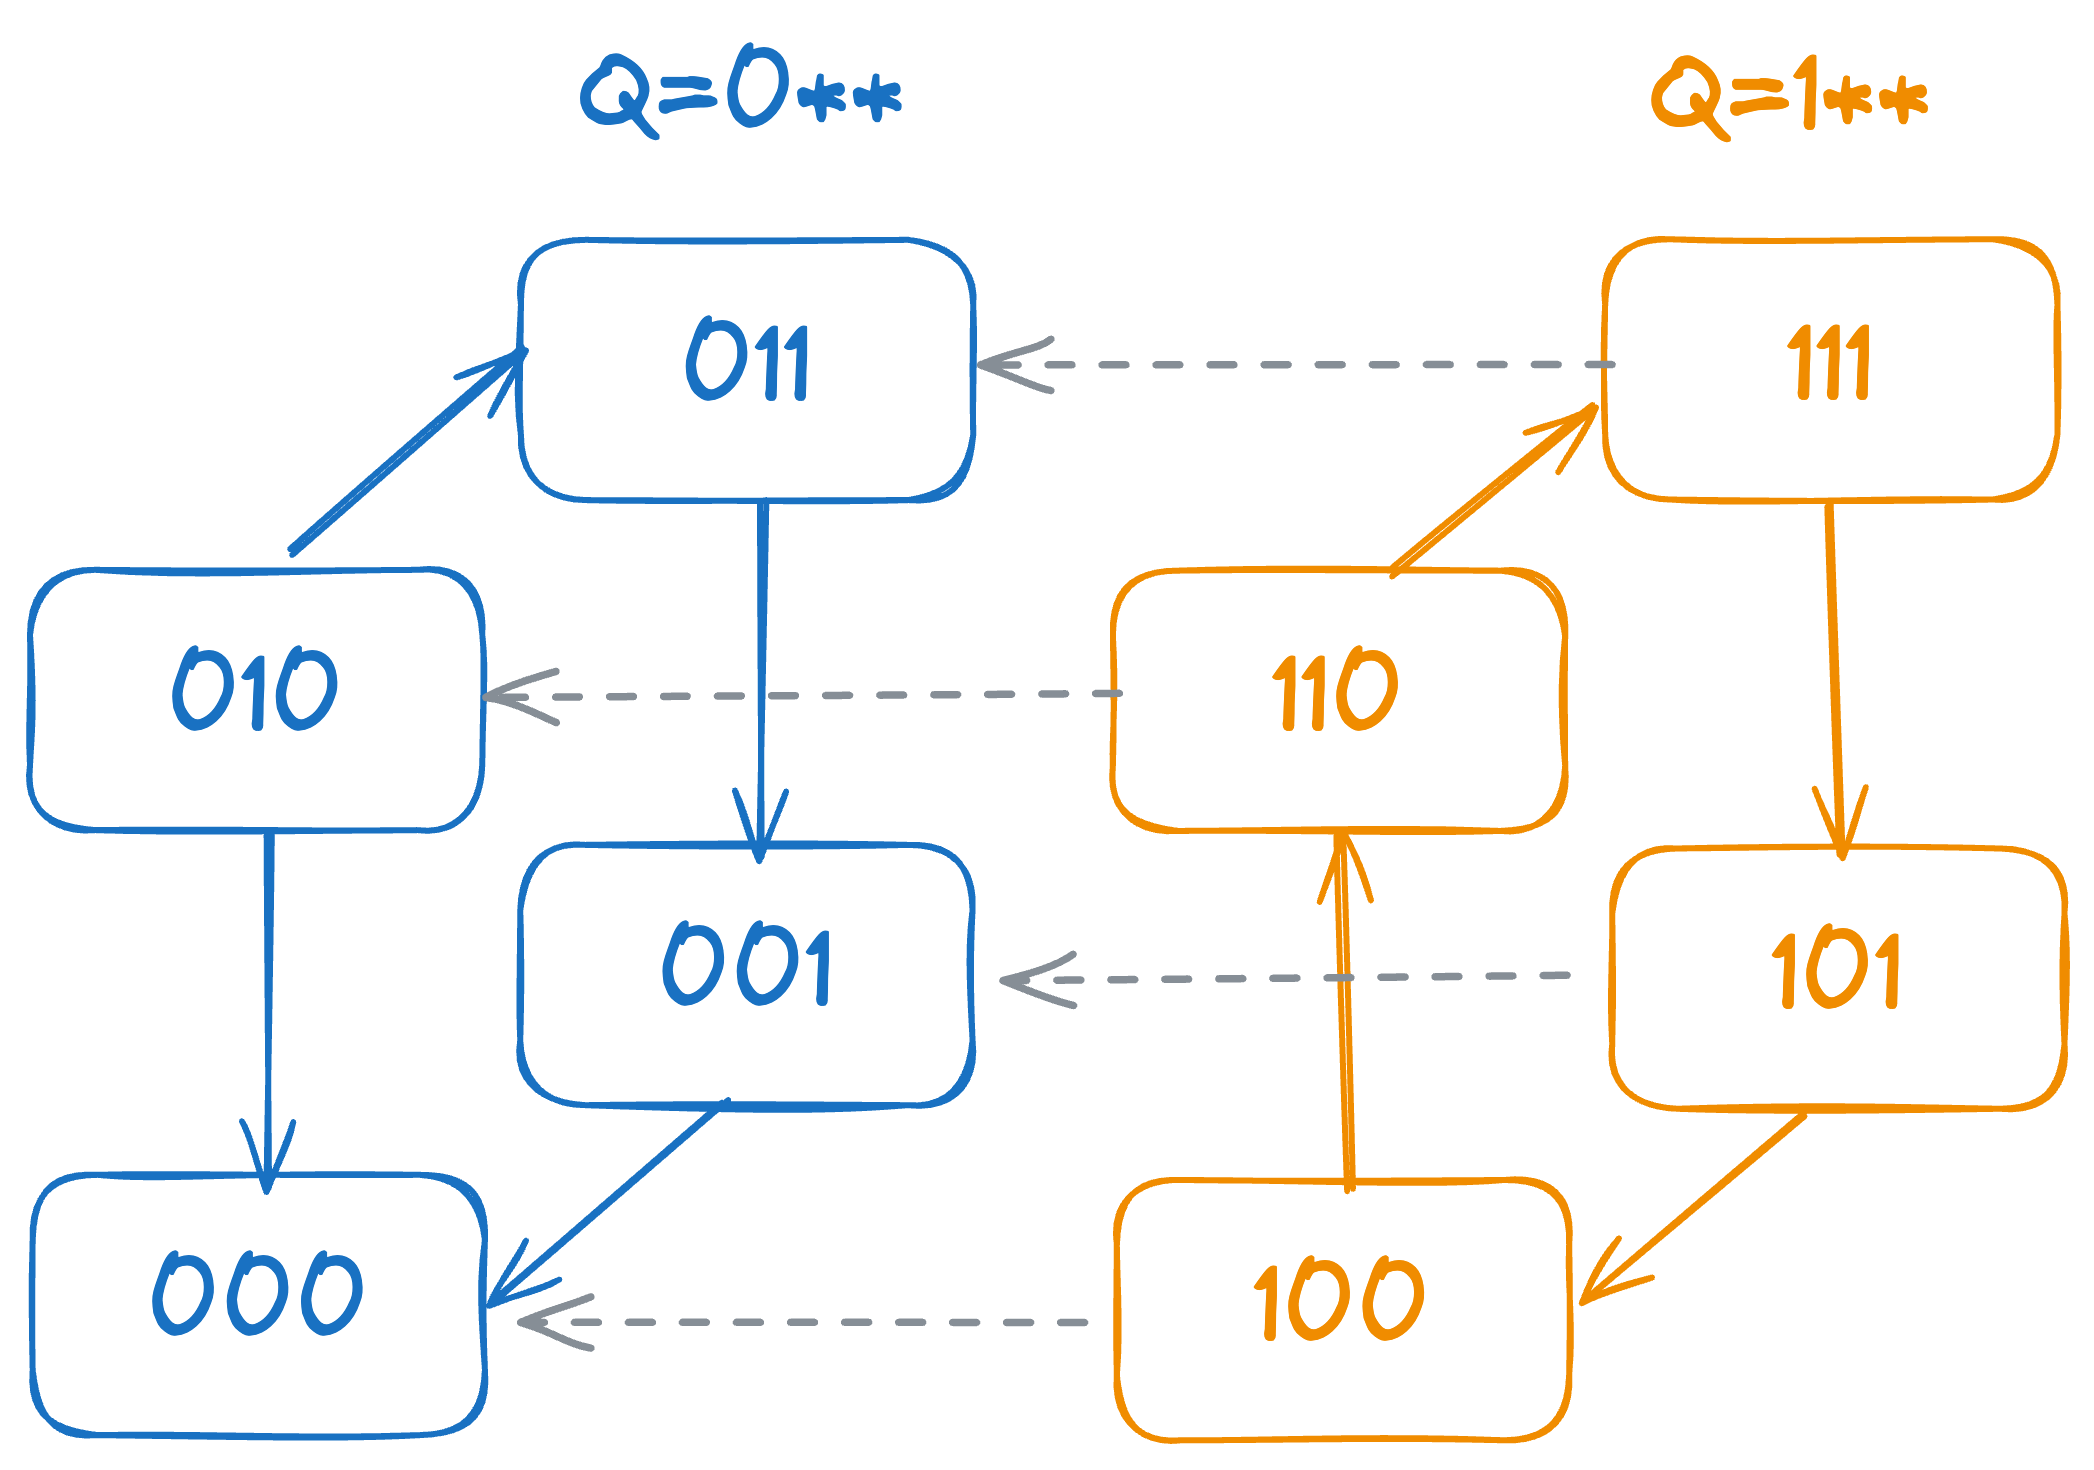
\includegraphics[width=.5\textwidth]{Figures/perturbation_encoding.png}	
		\caption{\textbf{Encoding of perturbations.} Illustration of how perturbations are encoded using pairs of network states and perturbation masks.}
		\label{fig:pert_encoding}
	\end{centering}
\end{figure}

Observe that this approach is more efficient than simply incorporating the set of all possible perturbations $\bools^n_*$ directly into the encoding. Each $\bools_*$ element would require more than one bit per network variable to encode, whereas our approach only adds one bit on top of the existing state space. The details of the decoding for the actual perturbations will be described in \autoref{subsec:supporting_algos}.

\subsection{Symbolic operations}
\label{subsec:symbolic_ops}

Aside from standard set operations ($\cap, \cup, \setminus, \times$, etc.), we also use $\exists_{\mathbb{L}}(X \subseteq \mathbb{X})$ to denote existential projection over the perturbed variables, i.e. $\exists_{\mathbb{L}}(X) = \{ (s, c) \mid \exists l \in \mathbb{L}~(s, c, l) \in X \}$. This can be implemented as a single operation on the directed graph of a BDD as well. Finally, we need a mechanism to symbolically explore the graph $\STG(\pbnMath)$ that is compliant with the applied variable perturbations. For this purpose, we define the following two operations:
\begin{align*}
      \pre(X \subseteq \mathbb{X}) =\; &\{ (s, \interpretation, l) \mid \exists (t, \interpretation, l) \in X \land s \not= t \\ &\land \exists i \in [1,n].t = s[i \mapsto f_i(s) \text{ of } \pbnMath(\interpretation)] \land  l_i = 0 \}\\
      \post(X \subseteq \mathbb{X}) =\; &\{ (t, \interpretation, l) \mid \exists (s, \interpretation, l) \in X \land s \not= t \\ &\land \exists i \in [1,n].t = s[i \mapsto f_i(s) \text{ of } \pbnMath(\interpretation)] \land l_i = 0 \}  
\end{align*}

Recall that the conditions above are almost exactly the condition under which $(v, \interpretation, u) \in E$ of $\STG(\pbnMath)$ (as per \autoref{def:psbn_perturbed_stg}). That is, $\pre$ and $\post$ compute the sets of predecessors and successors of the states in $X$ under their respective $\pbnMath$ interpretations. However, for each computed transition, we also require that $l_i = 0$, i.e. the $i$-th variable is \emph{not} perturbed. Hence values of the perturbed variables remain constant. For example, when $l_i = 1$ for all $i \in [1,n]$, no transition is possible. Meanwhile, when $l_i = 0$ for all $i \in [1,n]$, we get exactly the behaviour of $\STG(\pbnMath)$ without any perturbations. These two operations can also be implemented using BDDs, since $P_i$ is an expression over Boolean variables (which trivially corresponds to a Boolean function and hence a BDD). The rest are either pure logical operations or quantifications that can be realised as BDD operations.

\subsection{Supporting algorithms} 
\label{subsec:supporting_algos}

Our main algorithms rely on a collection of utility procedures defined in \autoref{algo:sb}. Before we proceed with the main result, we quickly explain the rationale behind these procedures. 

\begin{figure}[htp]
	\begin{centering}
		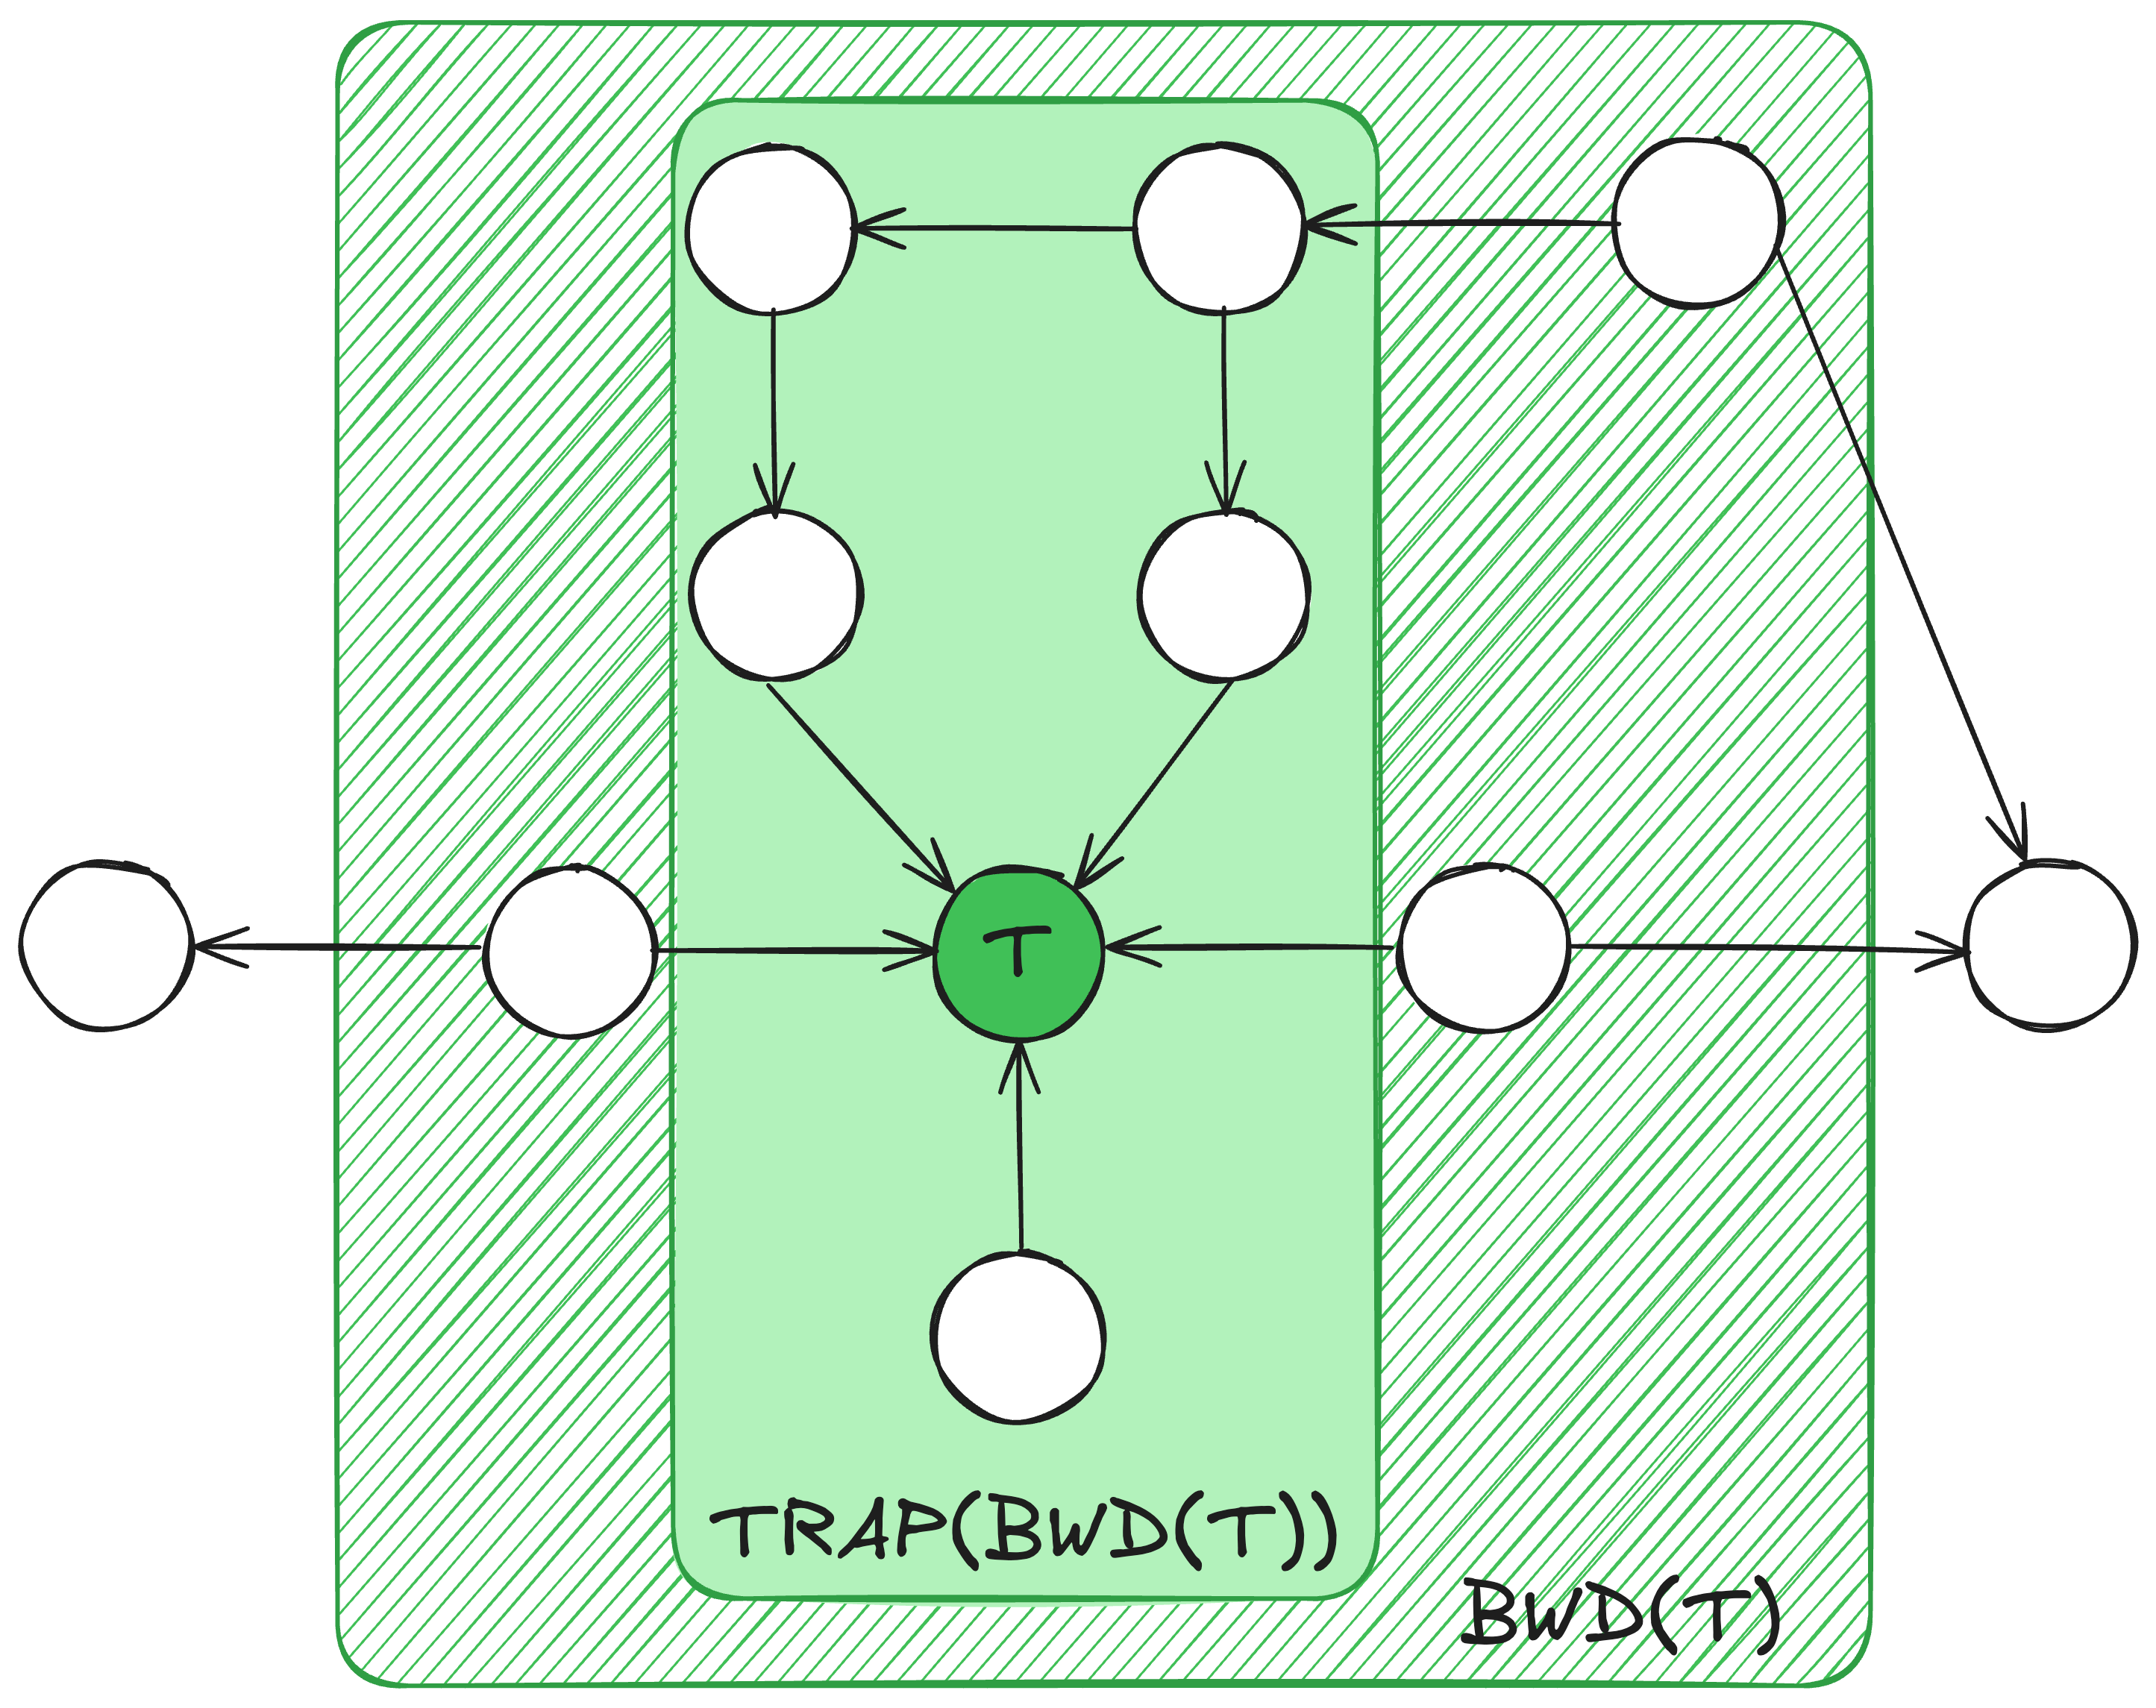
\includegraphics[width=.8\textwidth]{Figures/trap_bwd.png}	
		\caption{\textbf{$\bwd$ and $\fwdClosed$ procedures.} An intuitive example demonstrating the $\bwd$ and $\fwdClosed$ procedures from \autoref{algo:sb}. The highlighted dark green state is the target attractor state $T$. The shaded area represents the set of states $\bwd(\{T\})$ (weak basin of $T$). The solid green area represents the set $\fwdClosed(\bwd(\{T\}))$ (strong basin of $T$).}
		\label{fig:bn_trap_bwd}
	\end{centering}
\end{figure}

\paragraph{\bwd{}} This is a standard backward reachability procedure. That is, for the given set of initial states, it computes all transitive predecessors of these initial states. It also uses our modified notion of state space $\mathbb{X}$ which incorporates information about the perturbed variables. That is, if a variable is perturbed, it cannot be updates (recall our definition of $\textsc{Pre}$).

\paragraph{\fwdClosed{}} This procedure computes a generalized variant of \emph{trap sets} as defined in \autoref{section:boolean-networks}. The procedure takes a set of initial labelled states $X \subseteq \mathbb{X}$ and iteratively eliminates any components that have outgoing transitions leading out of $X$. For unperturbed components, this corresponds exactly to the notion of the trap set (grouped by possible interpretations encoded in the component $C$ of $\mathbb{X}$). For cases where the network is perturbed, the result is still a maximal subset of $X$ with no outgoing transitions, however, only with respect to the unperturbed variables.

\autoref{fig:bn_trap_bwd} shows an example demonstrating the use of $\bwd$ and $\fwdClosed$ (for simplicity, we do not consider multiple network interpretations or perturbations here). Given a target $t$ attractor state, the figure shows the set of all backwards reachable states $\bwd(\{t\})$ (weak basin of $t$). Set $\fwdClosed(\bwd(\{t\}))$ then depicts the maximal trap set contained within $\bwd(\{t\})$ (strong basin of $t$).

\paragraph{\textsc{CanPerturb}} %Finally, the most complex case is the procedure $\textsc{CanPerturb}$. 
Observe that while all procedures introduced so far \emph{respect} existing perturbations (by the means of the $\mathbb{L}$ component of $\mathbb{X}$), no procedure actually \emph{performs} the perturbation step from source $s$ to $\pertApply(s, \perturbation)$ as assumed by all three BN control approaches. However, since our control method works in a bottom up manner, we actually seek to answer a slightly modified question: given a set $T \subseteq \vertices$, what subset $T' \subseteq T$ is reachable from source $s$ by an admissible perturbation? Formally, the goal is to compute triples $(s, \interpretation, l) \in targets$ satisfying $\pertApply(source, \perturbation) = s$ for $\perturbation \equiv (s, l)$ (i.e. $\perturbation$ is the perturbation encoded within the $(s, \interpretation, l)$ triple).

\begin{algorithm}
	\SetKwProg{Fn}{Fn}{}{}
	\Fn{\upshape \bwd$(X \subseteq \mathbb{X})$}{
		\lRepeat{\upshape $X \textbf{ reaches fixpoint}$}{
			$X \gets X \cup \pre(X)$
		}
		\Return{$X$}\;
	} 
	\Fn{\upshape \fwdClosed$(X \subseteq \mathbb{X})$}{
		\tcc{Eliminate elements that escape from $X$ in one step.}
		\lRepeat{\upshape $X \textbf{ reaches fixpoint}$}{
			$X \gets X \setminus \pre(\post(X) \setminus X)$
		}
		\Return{$X$}\;
	}
	\Fn{\upshape \textsc{CanPerturb}$(\var{s} \in \vertices, \var{X} \subseteq \mathbb{X})$}{
		\For{$i \in \{ 1 \ldots n \}$}{
			$\var{diff}_i \gets \{~s' \in V \mid s'_i \not= \var{s}_i~\}$\; 
			$\var{unperturbed}_i \gets \{~l \in \mathbb{L} \mid l_i = 0~\}$\;
			$\var{X'} \gets \var{X} \setminus (\var{diff}_i \times \mathbb{L} \times \var{unperturbed}_i)$\;
		}
		\Return{\upshape $\var{X'}$}\;
	}
	\caption{Basic graph algorithms.}
	\label{algo:sb}x
\end{algorithm}    


To compute $\textsc{CanPerturb}(s, X)$, need we respect the following: Let $(s', \interpretation, l) \in X$ be a triple such that $s'_i \not= s_i$ and $l_i = 0$ for some $i \in [1,n]$. That is, source $s$ and $s'$ differ in the value of the $i$-th variable, but the variable is marked as unperturbed in $l$. Then, and only then we have that $\pertApply(s, \perturbation) \not= s'$ for $\perturbation \equiv (s, l)$. In other words, every $(s, c, l)$ for which such variable exists must be removed from $X$ when computing $\textsc{CanPerturb}$. \autoref{algo:sb} thus iterates through all network variables, constructing a symbolic representation of the set of triplets which violate the aforementioned condition, and subtracting this set from the original $X$. The result is a subset of the $X'$ relation where every member is reachable from source $s$ via its respective perturbation.

\subsection{Control algorithms}
\label{ss:control_algos_st_otp}

In \autoref{algo:permanent},  we describe the bottom-up procedures which compute the relations $\controlRelation_O$, $\controlRelation_P$, and $\controlRelation_T$. Each algorithm relies on the procedures from \autoref{algo:sb}, but incorporates specific adjustments to accommodate the temporal aspects of a specific control approach.

\begin{algorithm}
  \SetKwProg{Fn}{Fn}{}{}
  \Fn{\upshape \textsc{Permanent}$(\var{s} \in \vertices, \var{t} \in \vertices)$}{
    $\var{basin} \gets \fwdClosed(\bwd(\{ \var{t} \} \times \allInterpretations \times \mathbb{L}))$\;
    $\var{map} \gets \textsc{CanPerturb}(\var{s}, \var{basin})$\;
    \Return{\upshape $(\perturbation, \interpretation) \in \controlRelation_{P} \Leftrightarrow (s,\interpretation,l) \in \var{map} \land (s,l) \equiv \perturbation$}\;
  }
  \Fn{\upshape \textsc{OneStep}$(\var{s} \in \vertices, \var{t} \in \vertices)$}{
    $\var{basin} \gets \fwdClosed(\bwd(\{ \var{t} \} \times \allInterpretations \times \{ 0 \}^n))$\;
    $\var{basin} \gets \exists_\mathbb{L}(\var{basin}) \times \mathbb{L}$\;
    $\var{map} \gets \textsc{CanPerturb}(\var{s}, \var{basin})$\;
    \Return{\upshape $(\perturbation, \interpretation) \in \controlRelation_{O} \Leftrightarrow (\var{s},\interpretation,l) \in \var{map} \land (\var{s},l) \equiv \perturbation$}\;
  }
  \Fn{\upshape \textsc{Temporary}$(\var{s} \in \vertices, \var{t} \in \vertices)$}{
    $\var{basin} \gets \fwdClosed(\bwd(\{ \var{t} \} \times \allInterpretations \times \{ 0 \}^n))$\;
    $\var{basin} \gets \exists_\mathbb{L}(\var{basin}) \times \mathbb{L}$\;
    $\var{basin} \gets \fwdClosed(\bwd(\var{basin}))$\;
    $\var{map} \gets \textsc{CanPerturb}(\var{s}, \var{basin})$\;
    \Return{\upshape $(\perturbation, \interpretation) \in \controlRelation_{T} \Leftrightarrow (\var{s},\interpretation,l) \in \var{map} \land (\var{s},l) \equiv \perturbation$}\;
  }
  \caption{Control procedures.}
  \label{algo:permanent}
\end{algorithm}  

\paragraph{\textsc{Permanent}} The procedure for computing permanent control is the most straightforward. First, we use $\bwd(\{t\} \times \allInterpretations \times \mathbb{L})$ to determine all states that are able to reach $t$ across all possible PSBN interpretations ($\allInterpretations$) and combinations of perturbed variables ($\mathbb{L}$). Procedure $\fwdClosed$ then retains only the states from which all runs are guaranteed to eventually reach $t$. This follows from the fact that $t$ is a member of the only attractor within the initial set, hence fair runs that do not leave $\bwd(\{t\} \times \allInterpretations \times \mathbb{L})$ must eventually reach it. Finally, $\textsc{CanPerturb}$ is used to determine which of these cases are actually admissible under the given source $s$ . The result is a $\var{map} \subseteq \mathbb{X}$ which describes the control relation $\controlRelation_P$. As $\controlRelation_P$ is not a Boolean relation, it does not have a direct BDD representation---instead, the return statement describes how members of $\controlRelation_P$ correspond to the members of $map$. Intuitively, $map$ can be seen as a simple Boolean encoding of a non-Boolean relation $\controlRelation_P$. 

\paragraph{\textsc{One-step}} Since one-step control does not assume that perturbation is held over time, component $\mathbb{L}$ in the initial states is substituted for $\{ 0 \}^n$. This is a singleton set that only admits the case where no perturbation is applied. By computing $\fwdClosed(\bwd(\{t\} \times \allInterpretations \times \{0\}^n))$, we then get the combinations of states and interpretations which guarantee that $t$ is eventually reached (and visited infinitely often) in the unperturbed network. This corresponds to the strong basin of $t$.

Once $\var{basin}$ is computed, we cannot simply use $\textsc{CanPerturb}$ to identify possible perturbation candidates, as $basin$ only contains cases where the network is unperturbed. Instead, we use $\exists_{\mathbb{L}}(basin) \times \mathbb{L}$ to eliminate the $\{0\}^n$ component from the relation and substitute it for the full set $\mathbb{L}$. Intuitively, this enables all of the possible perturbations within the $basin$, allowing $\textsc{CanPerturb}$ to correctly select cases that are relevant for the given initial $s$ state.

\paragraph{\textsc{Temporary}} Finally, \textsc{Temporary} is conceptually a combination of both approaches: first, a $basin$ is computed with all perturbations disabled (i.e. $\{0\}^n$). At this point $basin$ represents the collection of possible states where lifting the perturbation guarantees that target $t$ is eventually visited infinitely often. Afterwards, $\{ 0 \}^n$ is exchanged for $\mathbb{L}$, which enables all possible perturbations in these $basin$ states. The combination of \bwd{} and \fwdClosed{} is then repeated, yielding a larger set of states that eventually always reach target $t$ even if the corresponding perturbation is initially applied, but eventually lifted (i.e. applied only temporarily). Finally, \textsc{CanPerturb} again limits this set to perturbations that are compatible with source $s$.

Note that under the assumption that $t$ is a member of an attractor for all $\interpretation \in \allInterpretations$, we have that the result of permanent control is always a subset of results for temporary control. Also note that for permanent control, if a combination of perturbed variables disturbs the attractor in which $t$ resides, the $\fwdClosed$ procedure ensures that such case is eliminated from the $basin$ relation entirely. This is because in this situation, all states (including $t$) can reach states that are not backwards reachable from $t$ and are thus eliminated.

Correctness of the procedures follows from the discussion above. All introduced procedures also surely terminate. The fixed-point procedures (\bwd{} and \fwdClosed{}) necessarily reach the fixed-point, because the superset $\mathbb{X}$ on which they operate is finite, and the resulting set can only grow (or shrink) in each iteration. The procedure \textsc{CanPerturb} is a straightforward for-loop over all BN variables. All control procedures are thus a composition of the described terminating operations or symbolic operations on BDDs.

\subsection{Evaluation}
\label{sec:control_evaluation}

To evaluate our methods, we have implemented algorithms from the previous section by using internal libraries of the tool AEON~\cite{aeon}. Our experiments were run using a computer with AMD Ryzen Threadripper 2990WX 32-Core Processor and 64GB of memory. We describe the software implementation and how to access it in the next chapter. %The repository also includes all auxiliary scripts we used for generating partially specified model versions, running the experiments, and visualizing their results.


\subsubsection{Benchmark model set} We use real-world biological BN models to evaluate our methods. The first model is a \emph{myeloid} differentiation network \cite{Krumsiek2011} which models a bone marrow tissue cell differentiation from common myeloid cells to specialised blood cells (megakaryocytes, erythrocytes, granulocytes and monocytes). The second model depicts heart development done by \emph{cardiac} kernel transcription factors~\cite{Waardenberg2014}. The third model explains regulatory interactions, which may cause \emph{ERBB} kinase over-expression -- a marker of breast cancer~\cite{Sahin2009}. The fourth model focuses on specific conditions which lead to a metastatic \emph{tumour}~\cite{Cohen2015}. The last model, the Mitogen-Activated Protein Kinase (\emph{MAPK}) network, consists of signalling pathways involved in diverse cellular processes, such as cell cycle, survival, apoptosis and differentiation~\cite{Grieco2013}. 

As our methods focus on the ability to handle systems with non-trivial unknown behaviour, we synthetically derive partially specified versions of the models listed above. We distinguish six model groups that differ in the number of interpretations (size of $\mid\allInterpretations\mid$). 

The numbers of interpretations corresponding to the individual groups are $[2^0,2^5], [2^6,2^{10}], \dots, [2^{26},2^{30}]$. For every class, we then generate 20 samples of partially specified networks by randomly removing some fully-specified functions. The arity of removed functions is limited to 5 to prevent intractable parameter explosion. This methodology approximates a uniform distribution of samples across an exponential scale of benchmark model sizes while still covering models with varying numbers and arity of uninterpreted functions. %tazky odsek :(

We then also randomly select the target and source attractor for every sampled model. However, we always verify that the actual number of model interpretations admitting the target attractor belongs to the given range. That is, for a model in class $2^{26}-2^{30}$, we guarantee that the target attractor is actually admissible for at least $2^{26}$ interpretations, even though the total number of all possible interpretations for the model can be higher. That is because we optimize control methods by restricting them to the interpretations where the attractor is present. As discussed in \autoref{ss:control_types_and_goal}, one-step and temporary controls are unable to stabilize a system in a state which is not part of any attractor. Since we want the results to be consistent for all methods and phenotypic variation is not the focus of this work, we pose the same constraint to permanent control.

\subsubsection{Scalability}

\begin{figure}[hbt!]
\checkoddpage
\edef\side{\ifoddpage l\else r\fi}
\makebox[\textwidth][\side]{% 
	\begin{minipage}{\fullwidth}
    \centering
    \subfloat[Myeloid (11 variables)~\cite{Krumsiek2011}]{
        \label{subfig:otp_results_a}
	\adjincludegraphics[trim={{0.75\width} 0 0 0},clip,width=0.33\textwidth]{Figures/myeloid_all.pdf}
    }
    \subfloat[Cardiac (15 variables)~\cite{Waardenberg2014}]{
        \label{subfig:otp_results_b}
	\adjincludegraphics[trim={{0.75\width} 0 0 0},clip,width=0.33\textwidth]{Figures/cardiac_all.pdf}
	}
    \subfloat[ERBB (20 variables)~\cite{Sahin2009}]{
        \label{subfig:otp_results_c}
	\adjincludegraphics[trim={{0.75\width} 0 0 0},clip,width=0.33\textwidth]{Figures/erbb_all.pdf}
	}
	\newline
    \subfloat[Tumour (32 variables)~\cite{Cohen2015}]{
        \label{subfig:otp_results_d}
	\adjincludegraphics[trim={{0.75\width} 0 0 0},clip,width=0.33\textwidth]{Figures/tumour_all.pdf}
	}
    \subfloat[MAPK (53 variables)~\cite{Grieco2013}]{
        \label{subfig:otp_results_e}
	\adjincludegraphics[trim={{0.75\width} 0 0 0},clip,width=0.33\textwidth]{Figures/mapk_all.pdf}
	}
    \caption{\textbf{Performance of the control methods.} Plots in every row show results for a different real-world model. The horizontal axis of all plots is showing the number of attractor colors (given by model instances from our benchmark set) and the vertical axis is for the duration (in ms) of the given method computation. Plots in the first three columns show all measurements for one-step, permanent and temporary controls using the colored markers which are surrounded by polygons to better visualize their disposition. The computations that did not finish computation within a threshold of 24 hours are not displayed in the figure. The last column displays scalability trends of all method results by interpolating logistic regression slope with $\log y = \log x$ function.} 
    \label{fig:otp_results}
	\end{minipage}
	}
\end{figure}

Our first experiment evaluates the performance and scalability of our method with respect to the model size (count of variables) and unknown knowledge (number of interpretations). We use the benchmark model set as described above. We list all results in \autoref{fig:otp_results}. All plots are showing the relation of method computation time to the number of considered attractor colors. The rows depict results for particular real-world models. In every column, there are results for different control methods (one-step, permanent, and temporary). The last column displays results from all methods in a single plot. To capture the scalability trends we use $\log y = \log x$ type of logistic regression (due to exponential scaling of colors as well as time). All computations had 24-hour time-out. Nonetheless, this case never occurred for one-step control and only in a MAPK model for permanent control (5 times). The temporary control yields more such cases, but only in the most demanding scenarios in ERBB (2 times), tumour (1 time) and MAPK (70 times) models. Note that as we disregard these results for compact logistic regression visualisation, the logistic regression might be slightly steeper in the reality.

% Our first experiment measures the performance of methods on five biological models with varying state space size (induced by the number of variables), number of interpretations, and possible number of perturbations. All these three components influence the size of the labelled graph under consideration. Whereas the number of vertices is equal to the number of states, the number of all STG instances is equivalent to the product of interpretations and possible perturbations. 

As described before, the symbolic representation is used to encode three types of entities: a set of the STG vertices, a set of interpretations (PSBN interpretations) which admit an edge in the STG, and a set of perturbations that permit the given edge. Therefore, when we increase the number of interpretations, only one dimension of the resulting symbolic representation grows. In opposition, when we increase the number of the system's variables, both the number of states and the number of available perturbations grow. Therefore, it is expected that increasing the model size has a bigger impact on the performance than increasing the number of model interpretations. This hypothesis is to some extent supported by our experiment captured in \autoref{fig:otp_results}. While the maximal increase of variables (myeloid vs. MAPK models) is just five-fold, we need to increase interpretations $10^7$ times to obtain the similar one-step control runtime of the myeloid model as the best-performing MAPK version. This difference is even amplified for other types of control. For example, in the case of temporary control, no myeloid model version performs as bad as the best-performing MAPK. 

Nonetheless, it must be highlighted that the impact of scaling up colours as well as variables is to some extent unpredictable. This is given by the intrinsic mechanics of the introduced STGs. As the nature of our method relies on fixed-point computation where each iteration eliminates only the direct predecessors of a particular set, in cases where e.g. a long path in the graph arises, our method will not be able to scale well: the algorithm will need many iterations to converge, each eliminating only a small fraction of the STG vertices. Another unforeseeable effect on the method's performance have the BDDs themselves. The ordering of the BDD diagram has a significant impact on the effectiveness of all operations and no single ordering strategy can perform best in all cases~\cite{Harlow2001}. Our observation is also supported by the experiment. 

Notice, the high variance of run times for the similar size of attractor interpretations shown in the plots. For example, in the case of temporary control in the ERBB model, compared to versions with fewest interpretations, some highest attractor interpretations (over $10^8$) cause just approximately $10$-times longer execution time while other cases with a similar number of interpretations result in time-outing computations, therefore the slow-down of over $10^7$. Or in the case of the myeloid model, even despite its somewhat smaller variable count than in the cardiac model, some computations take longer than in the bigger cardiac model, especially in the temporary control case. 

Another insight that can be obtained from \autoref{fig:otp_results} is how one-step, temporary and permanent controls differ in their complexity in terms of computational time. We can notice that one-step control is always over-performing other methods. This is because we do not need to consider perturbed state space when computing the trap set of the target attractor. In contrast, temporary control is usually by far the most computationally demanding compared to the other types of control. This should be given by the need to compute two trap sets. The first computed trap set is the same as in the case of one-step control and should be thus easy to compute. 

However, the seed for the second computed trap space is a much bigger vertex set, and therefore the resulting second trap space (which incorporates perturbations) of the first trap space (without perturbations) can generate much more complex symbolic structure and also gives more space for slowly converging fixed-points which were discussed previously. Nonetheless, in some rare cases with models containing few interpretations (myeloid and ERBB), the temporary control might over-perform the permanent one. This can be caused by the first (unperturbed) strong basin computed by temporary control being very similar to the second (perturbed one) while the first computation might be somewhat faster as it does not consider perturbations. We do not observe such scenarios in bigger models (tumor and MAPK)where the trends of one-step over-performing permanent control, and permanent over-performing temporary one look quite consistent.

\subsubsection{Robustness} 

Next, we conduct experiments evaluating the presented robustness metrics across different types of controls. In particular, we use maximal robustness $\rho_{max}$ and union robustness $\rho_{union}$ metrics which we measure on sets of fixed perturbation size. The results are shown in \autoref{fig:maximal_robustness} and \autoref{fig:total_robustness}. 

%For demonstration purposes, we selected just one arbitrary partially specified model instance for every real-world biological network from our benchmark model set, as the perturbation robustness across different randomized models is not directly comparable. 

\begin{figure}[htb!]
\checkoddpage
\edef\side{\ifoddpage l\else r\fi}
\makebox[\textwidth][\side]{% 
	\begin{minipage}{\fullwidth}
	\centering
	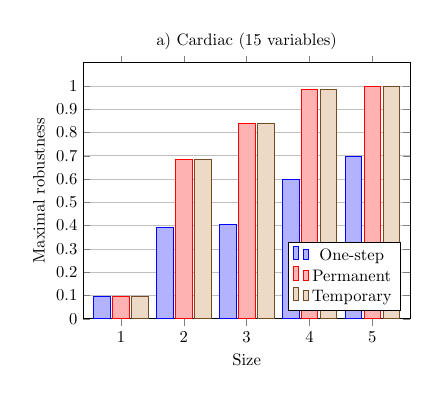
\begin{tikzpicture}[scale=0.6, transform shape]
	\begin{axis}[\axisStyle{a) Cardiac (15 variables)}{Maximal}]
		\addplot coordinates {(1,0.095)(2,0.393)(3,0.404)(4,0.599)(5,0.696)};
		\addplot coordinates {(1,0.095)(2,0.685)(3,0.841)(4,0.987)(5,1.0)};
		\addplot coordinates {(1,0.095)(2,0.685)(3,0.841)(4,0.987)(5,1.0)};
		\legend{One-step,Permanent,Temporary}
	\end{axis}
	\end{tikzpicture}
	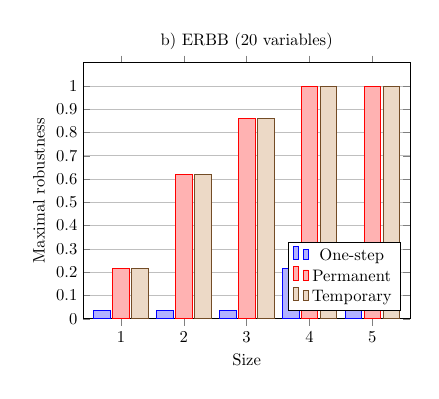
\begin{tikzpicture}[scale=0.6, transform shape]
	\begin{axis}[\axisStyle{b) ERBB (20 variables)}{Maximal}]
	\addplot coordinates {(1,0.034)(2,0.035)(3,0.036)(4,0.215)(5,0.240)};
	\addplot coordinates{(1,0.215)(2,0.621)(3,0.862)(4,1.0)(5,1.0)};
	\addplot coordinates{(1,0.215)(2,0.621)(3,0.862)(4,1.0)(5,1.0)};
	\legend{One-step,Permanent,Temporary}
	\end{axis}
	\end{tikzpicture}
	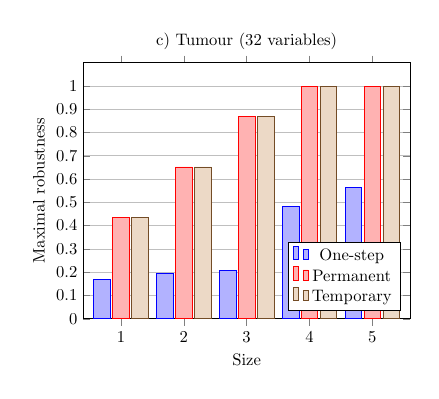
\begin{tikzpicture}[scale=0.6, transform shape]
	\begin{axis}[\axisStyle{c) Tumour (32 variables)}{Maximal}]
	\addplot coordinates {(1,0.169)(2,0.197)(3,0.209)(4,0.483)(5,0.563)};
	\addplot coordinates{(1,0.434)(2,0.652)(3,0.869)(4,1.0)(5,1.0)};
	\addplot coordinates{(1,0.434)(2,0.652)(3,0.869)(4,1.0)(5,1.0)};
	\legend{One-step,Permanent,Temporary}
	\end{axis}
	\end{tikzpicture}
	\caption{Maximal robustness $\rho_{max}$ per set of perturbations with a given size -- comparison between different types of controls. The horizontal axis shows the size of perturbations in the set and the vertical axis displays the maximal robustness. Each chart is showing robustness for a different model.}
	\label{fig:maximal_robustness}
	\end{minipage}
}
\end{figure}

\begin{figure}[htb!]
\checkoddpage
\edef\side{\ifoddpage l\else r\fi}
\makebox[\textwidth][\side]{% 
	\begin{minipage}{\fullwidth}
	\centering
	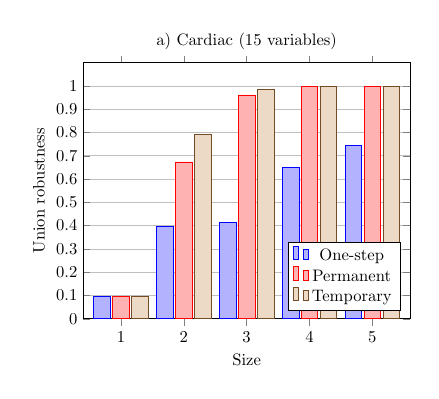
\begin{tikzpicture}[scale=0.6, transform shape]
	\begin{axis}[\axisStyle{a) Cardiac (15 variables)}{Union}]
	\addplot coordinates {(1,0.095)(2,0.395)(3,0.414)(4,0.649)(5,0.743)};
	\addplot coordinates {(1,0.095)(2,0.674)(3,0.962)(4,0.999)(5,1.0)};
	\addplot coordinates {(1,0.095)(2,0.792)(3,0.986)(4,0.999)(5,1.0)};
	\legend{One-step,Permanent,Temporary}
	\end{axis}
	\end{tikzpicture}
	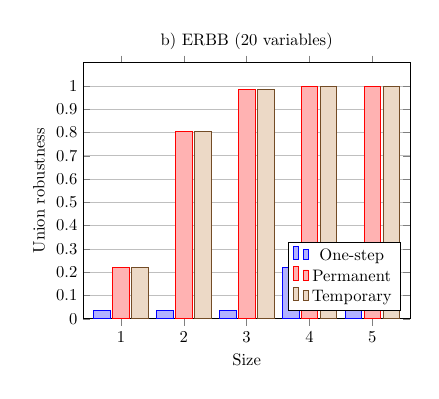
\begin{tikzpicture}[scale=0.6, transform shape]
	\begin{axis}[\axisStyle{b) ERBB (20 variables)}{Union}]
	\addplot coordinates {(1,0.035)(2,0.036)(3,0.036)(4,0.220)(5,0.252)};
	\addplot coordinates {(1,0.220)(2,0.806)(3,0.985)(4,1.0)(5,1.0)};
	\addplot coordinates {(1,0.220)(2,0.806)(3,0.985)(4,1.0)(5,1.0)};
	\legend{One-step,Permanent,Temporary}
	\end{axis}
	\end{tikzpicture}
	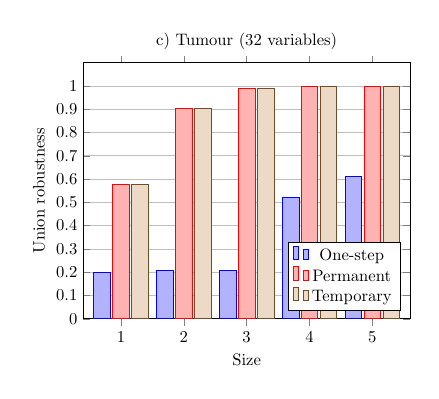
\begin{tikzpicture}[scale=0.6, transform shape]
	\begin{axis}[\axisStyle{c) Tumour (32 variables)}{Union}]
	\addplot coordinates {(1,0.198)(2,0.208)(3,0.209)(4,0.523)(5,0.610)};
	\addplot coordinates {(1,0.576)(2,0.902)(3,0.991)(4,1.0)(5,1.0)};
	\addplot coordinates {(1,0.576)(2,0.902)(3,0.991)(4,1.0)(5,1.0)};
	\legend{One-step,Permanent,Temporary}
	\end{axis}
	\end{tikzpicture}
	\caption{Union robustness $\rho_{\cup}$ per set of perturbations with a given size -- a comparison between different types of controls. The horizontal axis shows the size of perturbations in the set and the vertical axis displays the union robustness. Each chart is showing robustness for a different model.}
	\label{fig:total_robustness}
	\end{minipage}
}
\end{figure}

% Apart from the time-wise performance, we also compared the robustness of different types of control (see \autoref{fig:maximal_robustness} and \autoref{fig:total_robustness}). 

First, let us look at what particular types of global robustness metrics can tell us about the inspected systems. Under the assumption that the real biological system corresponds to a single ``correct'' interpretations of our partially specified BN model, what the maximal robustness tells us is how high the chance that \emph{a particular perturbation} will work in the real model. Alternatively, we use union robustness to evaluate a chance that there is \emph{some perturbation} of the given size that will work. For example, in the ERBB model (\autoref{fig:maximal_robustness}b and \autoref{fig:total_robustness}b), we can notice that there is a 60\% chance that the most robust perturbation (temporary or permanent) of size two will work for the real, fully specified model. However, even if this particular perturbation fails, we know that 80\% of the interpretations can be influenced by a perturbation of this size. This means that out of the 40\% of interpretations that cannot be influenced by the perturbation with the maximal robustness, half is still controllable by perturbing only two variables. For all three models, it is thus highly likely that a temporary perturbation of size no bigger than 3 exists which controls the network. That is a very small portion of the total model variables which could be possibly perturbed.

As the one-step control is subsumed by temporary control, it is expected that the temporary perturbations achieve the same or higher robustness than the one-step perturbations. This is also shown in the experiments, where we find no instance in which the one-step control could achieve higher maximal or union robustness. We can also observe that temporary and permanent controls mostly perform very similarly. 

Specifically, they achieve 100\% maximal robustness for perturbations of size three (in the case of the cardiac model) or four (in the case of other models). Therefore, we successfully computed perturbations which surely work even despite the missing knowledge we introduced into the models for the purpose of our experiments. This is also in line with previous research demonstrated by, e.g.,~\cite{Su2019CMSB, Su2020}, where the necessary size of temporary or permanent control is often very small.

The temporary control outperforms the permanent in the union robustness only in the cardiac model (\autoref{fig:total_robustness}a). This means there are some perturbations which work when applied temporarily as opposed to when applied permanently. The possible reasons for this were already discussed in the previous sections. Nonetheless, there are two admissible explanations. 

The first may be a simple fact that the trap set computed for temporary control is expected to be bigger since the seed of the trap set is not only the given target state but also its unperturbed trap set. The second explanation for this is a scenario when a permanent perturbation disrupts the BN dynamics in such a way that the target attractor becomes unreachable or completely ceases to exist. Our observation is also in line with~\cite{Su2019FM}, where the minimal temporary control also outperformed the permanent one in a few cases.


\subsubsection{Comparison of source-target methods}
\label{sec:comparison_source_target}

\begin{figure}[htbp!]
	\checkoddpage
	\edef\side{\ifoddpage l\else r\fi}
	\makebox[\textwidth][\side]{% 
	\begin{minipage}{\fullwidth}
    \centering
    \subfloat[Myeloid (11 variables)~\cite{Krumsiek2011}]{
        \label{subfig:benchmarks_os_a}
	\adjincludegraphics[trim={{0.66\width} 0 0 0},clip,width=0.33\textwidth]{Figures/myeloid_os.pdf}
    }
    \subfloat[Cardiac (15 variables)~\cite{Waardenberg2014}]{
        \label{subfig:benchmarks_os_b}
	\adjincludegraphics[trim={{0.66\width} 0 0 0},clip,width=0.33\textwidth]{Figures/cardiac_os.pdf}
	}
    \subfloat[ERBB (20 variables)~\cite{Sahin2009}]{
        \label{subfig:benchmarks_os_c}
	\adjincludegraphics[trim={{0.66\width} 0 0 0},clip,width=0.33\textwidth]{Figures/erbb_os.pdf}
	}
    \caption{\textbf{Comparison with existing semi-symbolic method from~\cite{Brim2021}.} Plots in every row show results for a different real-world model. The horizontal axis of all plots shows the number of attractor interpretations (given by model instances from our benchmark set) and the vertical axis is for the duration (in ms) of the given method computation. Both axes have logarithmic scaling. Plots in the first column show all measurements for the fully symbolic one-step method from this work. The second plot is showing results for the one-step control method from~\cite{Brim2021} using the colored markers. Plots display scalability trends of all methods by interpolating the results with the logistic regression slope of $\log y = \log x$ function.}
    \label{fig:benchmarks_os}
	\end{minipage}
}
\end{figure}

We also compare the symbolic and the semi-symbolic approach described in the previous \autoref{sec:target_semisymbolic} (from~\cite{Brim2021}) one-step controls. The results are captured in \autoref{fig:benchmarks_os}. We use the same benchmark model set as in the previous experiment. We also use a similar layout for plots in the figure. 

However, there are fewer rows as the semi-symbolic method was not able to compute any instance of tumor or MAPK models due to out-of-memory (OOM) errors. Also, some instances of ERBB model were not processed due to OOM rather than time-outs. The first column shows the results of the fully symbolic one-step control method while the second column shows the results of the previous semi-symbolic method. The plots in the last column compactly compare these two methods using the same logistic regression as in the previous experiment.



% Experiment 2 - A bridge to related work
Another insight of our experiments is a comparison of the novel symbolic approach to the semi-symbolic approach from~\cite{Brim2021}. The experiment captured in \autoref{fig:benchmarks_os} shows that the symbolic approach is performing better in all measured cases. As can be seen from the regression trends, the bigger the model, the bigger is also the margin by which the novel method over-performs the semi-symbolic one. However, in the highly parametrised cases, the parallelization of the semi-symbolic method might be faster than the fully symbolic one. This is also suggested by the linear regression trends where we can notice, that the semi-symbolic method has a less steep slope. Nonetheless, the greatest benefit of our novel method is the ability to process models with significantly bigger state space such as the tumor model or MAPK, as well as the highly unknown variants of the ERBB model, where the explicit state-space considered by the semi-symbolic approach completely fails to fit into the available memory.

\subsection{Summary}
\label{s:discussion}


 In this section we have presented novel fully symbolic methods for solving the source-target control problem for partially specified BNs. We have described the algorithms for computing one-step, temporary and permanent control relations. Finally, we have evaluated our methods on a benchmark set of real-world biological models with varying sizes and degrees of uncertainty. We have compared the performance of different types of control and also compared our one-step control method to the semi-symbolic approach from \autoref{sec:target_semisymbolic}. We have shown, that new symbolic methods are superior in both performance and scalability, as well as in the size of perturbations enabled by temporary and permanent control.

% In this work, we have developed methods and efficient algorithms to solve the source-target control problem for partially specified BNs using one-step, temporary and permanent state perturbations. The methods we proposed are entirely symbolic and are based on BDDs. We demonstrated that our approach is capable of controlling models with a high degree of uncertainty in a conveniently short time. Such a result
% cannot be achieved with the na\"ive scan over all BN parameters due to the doubly exponential explosion of the number of parameters representing the fully specified BN instances. We also showed that our novel methods are superior to the existing semi-symbolic one-step control approach~\cite{Brim2021}. We were also able to evaluate robustness between different types of control thanks to the metrics we introduced: maximal and union robustness.


% Related work
% Finally, let us compare our results with the related work discussed in \autoref{s:introduction}. It is important to note that the previously published methods other than~\cite{Brim2021} do not support partially specified BNs. Therefore, we deem our method incomparable to the previous line of research in terms of performance. Hypothetically, the other methods could be used to iteratively process all interpretations of a partially specified BN, resulting in a na\"ive parameter-scan approach. Nonetheless, as the number of interpretations grows exponentially, this approach cannot scale in the same way and thus quickly becomes infeasible. More than that, our approach allows easy evaluation of robustness, which would otherwise also be more complicated when the results are computed na\"ively. Considering other aspects of BN control, our method supports all types of static perturbations (one-step, temporary, permanent)~\cite{Su2020}. However, it does not support more complex, dynamical applications of sequential perturbations~\cite{Mandon2019CMSB, Su2020}. With sequential perturbations, it is possible to achieve minimal perturbations of even smaller sizes. However, we consider such an approach too computationally demanding for the case of partially specified BNs at the moment---the combinatorial space of available perturbations, colours, and attractors (each present only for a subset of colours) would be enormous. Finally, our method supports only source-target control. We leave other types of control, e.g., the target control~\cite{Su2020BCB} and the phenotype control~\cite{Fontanals2022b} for future work.


\chapter{Phenotype Control of Partially Specified Boolean Networks}
\label{chapter:phenotype_control_psbn}

% \begin{enumerate}
%     \item CMSB2023
%     \item What? why?
%     \item Robustness
%     \item Algorithm
%     \item Example
%     \item Performance/scalability
% \end{enumerate}


Finally, we can discuss the topic of phenotype control for PSBNs: we assume a set of phenotype states $P \subseteq \bools^n$ and the goal is to perturb the network such that it \emph{exhibits} this phenotype. In other words, after the perturbation is applied to the network, the network stabilizes in some attractor $A$ such that $A \subseteq P$. However, in the presence of partially unknown dynamics, this may not be achievable using a sufficiently small perturbation. In such cases, we rely on control \emph{robustness} to assess viability of possible perturbations.

\section{Problem Definition}
\label{s:phenotype_problem_definition}

As before, for simplicity, we first introduce some of the concepts for classical BNs and then expand these to PSBNs. First, to control the behaviour of a BN, we use the notion of variable perturbation:

\begin{definition}
	A \emph{variable perturbation} is a vector $Q \in \bools_\unspecified^n$. For every $Q_i = {\unspecified}$, we say that the $i$-th variable is \emph{unperturbed}, whereas for $Q_i = 0$ or $Q_i = 1$, we say the variable is \emph{perturbed} to either $0$ or $1$.
\end{definition}

We write $\mathit{fixed}(Q)$ and $\mathit{free}(Q)$ to denote the subset of perturbed and unperturbed variables, respectively. The \emph{size} of $Q$ is the size of the $\textit{fixed}(Q)$ set. Furthermore, a perturbation can again be seen as a \emph{subspace} of $\bools^n$. We then write that the states in this subspace are \emph{compliant} with $Q$.

For a particular $\mathbb{BN}$ and $Q$, we consider a \emph{perturbed} state-transition graph $\STG[Q](\mathbb{BN})$, which is a sub-graph of $\STG(\mathbb{BN})$ \emph{induced} by the states compliant with $Q$. Intuitively, the $\mathit{fixed}(Q)$ variables are restricted to their perturbed values, while $\mathit{free}(Q)$ variables are left to evolve without modification. 

%\begin{definition}
We say that a~permanent variable perturbation $Q \in \bools_\unspecified^n$ \emph{controls} Boolean network $\mathbb{BN}$ towards phenotype $P$ if and only if $\mathcal{A}(\STG[Q](\mathbb{BN})) \subseteq P$.
%\end{definition}
Intuitively, a perturbation represents an effective control strategy if it causes the network to only exhibit attractors from the desired phenotype $P$. However, note that $\mathcal{A}(\STG[Q](\mathbb{BN}))$ is not necessarily a subset of $\mathcal{A}(\STG(\mathbb{BN}))$. A permanent perturbation can disturb existing attractors or even introduce new ones.

This concept naturally applies to interpretations of PSBNs as well: given a $\mathbb{PSBN}$, an interpretation $\mathcal{I}$ and a perturbation $Q$, the interpretation has a perturbed $\STG[Q](\mathbb{PSBN}(\mathcal{I}))$. As such, a perturbation $Q$ controls $\mathbb{PSBN}$ under the interpretation $\mathcal{I}$ if it ensures $\mathcal{A}(\STG[Q](\mathbb{PSBN}(\mathcal{I}))) \subseteq P$.

\begin{example}
	Consider the network from \autoref{example:psbn}, a phenotype $P = 1 \unspecified \unspecified$ and a perturbation $Q = \unspecified 1  \unspecified$. \autoref{subfig:perturbed_stg} depicts the perturbed STGs of interpretations $\mathcal{I}_{0101}$ and $\mathcal{I}_{0110}$, with phenotype states highlighted in green. Perturbation $Q = \unspecified 1  \unspecified$ achieves control for interpretation $\mathcal{I}_{0101}$, but not for $\mathcal{I}_{0110}$.
\end{example}

\begin{definition}
	Assume a partially specified network $\mathbb{PSBN}$, a phenotype $P \subseteq \bools^n$ and a set of admissible perturbations $\mathcal{Q} \subseteq \bools_\unspecified^n$. The goal of the \emph{complete} phenotype control is to compute all pairs $(c, Q) \in \bools^m \times \bools_\unspecified^n$ such that $Q \in \mathcal{Q}$ and $Q$ controls $\mathbb{PSBN}(\mathcal{I}_c)$ towards phenotype $P$.
\end{definition}

Intuitively, the result of PSBN phenotype control are all combinations of colours and perturbations for which the perturbation necessarily stabilizes the associated network interpretation in the given phenotype. The set $\mathcal{Q}$ is in practice used to restrict the problem setting to perturbations of a certain size or to otherwise biologically feasible perturbations.

\paragraph{Perturbation size and robustness}

In practice, it is often unnecessary to compute the complete set of colour-perturbation pairs. The goal is instead to find the smallest functioning perturbation~\cite{Su2019CMSB,Su2020}. However, in partially specified networks, such minimal perturbation typically only works for a small subset of interpretations, making it potentially unreliable in practice. To address this, we consider robust phenotype control:

\begin{definition}
	The \emph{robustness} $\rho$ of a perturbation $Q \in \bools_\unspecified^n$ is defined as:
	\begin{align*}
		\rho(Q) = \frac{|\{ c \in \bools^{m} \mid Q~\text{\upshape controls}~\mathbb{PSBN}(\mathcal{I}_c) \}|}{|\bools^{m}|}
	\end{align*}
	Given a robustness threshold $r \in (0,1]$, the goal of \emph{robust} phenotype control is to compute the smallest perturbation (or perturbations) $Q$ s.t. $\rho(Q) \geq r$.
\end{definition}

Ideally, a suitable perturbation $Q$ with $\rho(Q) = 1$ achieves control for all interpretations of $\mathbb{PSBN}$. However, if no such perturbation exists, the parameter $r$ can be tuned to achieve a trade off between perturbation size and robustness.

\section{Methods}
\label{sec:Methods}

%TODO: Vyzdvihnut, co je rovnake z Biosystems2023

Partially specified Boolean networks suffer from both state and parameter space explosion, which in practice makes them hard to analyse exhaustively. In the context of control, this problem is further complicated by perturbation space explosion. To mitigate this, we employ symbolic state space exploration which allows us to analyse the full set of possible perturbed STGs within a single algorithm pass. This technique exploits similarities between the STGs of various network interpretations (and perturbations) to significantly speed up the exploration process compared to the naive enumeration~\cite{aeonpy,Brim2021}.

\subsection{Symbolic computation model}

A binary decision diagram (BDD)~\cite{Bryant86} is a directed acyclic graph which represents a Boolean function. A BDD-encoded function $f: \bools^k \to \bools$ can be used to encode a set (or relation) of Boolean vectors $X \subseteq \bools^k$, such that $f(x) = 1 \Leftrightarrow x \in X$. Since both network states ($\bools^n$) and interpretations ($\bools^m$ after normalisation) correspond to Boolean vectors, such sets have a direct BDD representation.

For sets of perturbations, a naive approach requires two Boolean variables per component, since their domain is $\bools_\unspecified$ instead of $\bools$. However, in~\cite{brim2022}, we introduce an alternative encoding suitable for representing perturbed state-transition systems that only requires one variable. This significantly improves the efficiency of the encoding, since fewer symbolic variables typically result in smaller BDDs.

\paragraph{Perturbed STG encoding} Observe that in the context of a state $x \in \bools^n$ which is \emph{compliant} with a perturbation $Q$, it is sufficient to know the set $\mathit{fixed}(Q)$ to fully reconstruct $Q$: we have $Q_i = x_i$ for every $i \in \mathit{fixed}(Q)$ and $Q_i = \unspecified$ otherwise. 

Consequently, a relation over states $x$, interpretations $\mathcal{I}_c$ and perturbations $Q$ where all states are compliant with their respective perturbations can be encoded as a relation over $\bools^n \times \bools^m \times \bools^n$. Here, the last component encodes the possible sets $\mathit{fixed}(Q)$. Since each perturbed $\STG[Q](\mathbb{BN})$ only admits states compliant with $Q$, such representation is suitable for collectively encoding dynamics of such perturbed STGs for different perturbations. 

To avoid confusion, we write $\mathcal{V} \equiv \bools^n$ to mean the set of network states, $\mathcal{C} \equiv \bools^m$ to mean the set of network interpretations (colours), and $\mathcal{L} \equiv \bools^n$ to mean the set of sets of perturbed variables $\mathit{fixed}(Q)$, collectively $\mathcal{S} = \mathcal{V} \times \mathcal{C} \times \mathcal{L}$. For $(x,l) \in \mathcal{V} \times \mathcal{L}$, we also write that $Q \equiv (x,l)$ when $Q_i = x_i$ for all $l_i = 1$ and $Q_i = \unspecified$ when $l_i = 0$ (i.e. $Q$ can be reconstructed based on the state $x$ and the set of perturbed variables $l$). 

When the goal is to symbolically represent a subset of perturbations $\mathcal{Q} \subseteq \bools_\unspecified^n$, we do this through a relation $S_{\mathcal{Q}} \subseteq \mathcal{V} \times \mathcal{L}$ where $S_{\mathcal{Q}}$ contains exactly \emph{all} states compliant with every $Q \in S$. Finally, in some cases, we may need to directly reference the Boolean BDD variables used in our encoding. We then use the notation $\mathcal{V}_i$, $\mathcal{C}_i$, resp. $\mathcal{L}_i$ to denote the $i$-th BDD variable that encodes the state, colour or perturbation component of $\mathcal{S}$.

\paragraph{Symbolic operations} Set operations ($\cap, \cup, \setminus$, etc.) on symbolic sets (or relations) are implemented through Boolean logical operators ($\land, \lor, \neg$, etc.) as is customary for BDDs. Furthermore, the following standard BDD operations are used:
\begin{align*}
	\textsc{Project}_{\mathcal{X}}(X \subseteq \mathbb{B}^k)&= \{ x \in \mathbb{B}^k \mid \exists b \in \bools.~x[\mathcal{X} \mapsto b] \in X \}\\
	\textsc{Select}_{\mathcal{X}=b}(X \subseteq \mathbb{B}^k)&= \{ x \in \mathbb{B}^k \mid x \in X \land x[\mathcal{X}] = b \}\\	
	\textsc{Restrict}_{\mathcal{X}=b}(X \subseteq \mathbb{B}^k)&=\textsc{Project}_{\mathcal{X}}(\textsc{Select}_{\mathcal{X}=b}(X))
\end{align*}

Here, $\mathcal{X}$ denotes a variable of the BDD encoding (e.g. $\mathcal{V}_3$). We can also use a list of conditions in the subscript of the method as a shorthand for multiple nested calls to the same method. Intuitively, $\textsc{Project}$ is equivalent to existential quantification, $\textsc{Select}$ is implemented through conjunction, and $\textsc{Restrict}$ is a combination of both. To explore the perturbed STGs, we use:
\begin{align*}
      \pre(X \subseteq \mathcal{S}) &= \{~(s, c, l) \mid \exists (t, c, l) \in X.~s \to_{c,Q}^{} t \text{ for } Q \equiv (s, l)~\}\\
      \post(X \subseteq \mathcal{S}) &= \{~(t, c, l) \mid \exists (s, c, l) \in X.~s \to_{c,Q}^{} t \text{ for } Q \equiv (s, l)~\}
\end{align*}
Here, $s \to_{c,Q} t$ denotes that $s \to t$ within the graph $\STG[Q](\mathbb{PSBN}(\mathcal{I}_c))$. Intuitively, $\pre$ and $\post$ compute the sets of predecessors and successors of the states in $X$ within $\mathbb{PSBN}$ under their respective interpretations $\mathcal{I}_c$ and perturbations $Q$. The implementation details of these operations can be found in~\cite{brim2022}.

We then rely on a method $\textsc{Trap}(X \subseteq \mathcal{S})$ which computes the \emph{maximal trap set} within the given set $X$. Naively, this method can be implemented as the greatest fixed point of $\textsc{Trap}(X) = X \cap \textsc{Trap}(X \setminus \textsc{Pre}(\textsc{Post}(X)))$. However, we use a more efficient implementation based on the technique called \emph{saturation}~\cite{benevs2022bdd}.

Finally, we use $\mathbb{VAL}_k^n$ to denote a BDD which encodes a function of $n$ inputs that is $\mathit{true}$ iff exactly $k$ inputs are $\mathit{true}$. To construct such BDD efficiently, we observe that $\mathbb{VAL}_0^n = \bigwedge_{i \in [1,n]} \neg x_i$, and that $\mathbb{VAL}_k^n = \bigvee_{i \in [1,n]} (\mathbb{VAL}_{k-1}^n \lor x_i)$.

\subsection{Control algorithm}

Our control approach is based on \autoref{algo:control} where we describe:

\begin{itemize}
	\item $\textsc{CompletePhenotypeControl}$: Core algorithm that iteratively computes the \emph{complete} control map for an admissible set $\mathcal{Q}$.
	\item $\textsc{RobustPhenotypeControl}$: A wrapper for the core algorithm that facilitates minimal control under the desired \emph{robustness}.
	\item $\textsc{Enumerate}$: An auxiliary method to enumerate all \emph{working} perturbations and find the maximum robustness.
\end{itemize}


\begin{algorithm}[ht!]
  \SetKwProg{Fn}{Fn}{}{}
	\Fn{\upshape \textsc{CompletePhenotypeControl}$(P \subseteq \mathcal{V}, \mathcal{Q} \subseteq \mathcal{V} \times \mathcal{L} ~(\text{encodes~}\bools_\unspecified^n))$}{
		$\var{universe} \gets \{~(x, c, l) \in \mathcal{S} \mid (x,l) \in \mathcal{Q}~\}$\;
		$\var{phenotype} \gets \var{universe} \cap (P \times \mathcal{C} \times \mathcal{L})$\;
		$\var{phenotype\_trap} \gets \textsc{Trap}(\var{phenotype})$\;
		$\var{non\_phenotype} \gets \var{universe} \setminus \var{phenotype\_trap}$\;
		$\var{cannot\_control} \gets \textsc{Trap}(\var{non\_phenotype})$\;
		\For{$i \in [1,n]$}{
			$\var{not\_perturbed} \gets \textsc{Project}_{\mathcal{V}_i}(\textsc{Select}_{\mathcal{L}_i = 0}(\var{cannot\_control}))$\;
			$\var{cannot\_control} \gets \var{not\_perturbed} \cup \textsc{Select}_{\mathcal{L}_i = 1}(\var{cannot\_control})$\;
		}
		$\var{control\_map} \gets \var{universe} \setminus \var{cannot\_control}$\;
		\Return{\upshape$\var{control\_map}$}\;
	}
	\Fn{\upshape \textsc{RobustPhenotypeControl}$(r, P \subseteq \mathcal{V}, \mathcal{Q} \subseteq \mathcal{V} \times \mathcal{L})$}{
		\For{$k \in [0,n]$}{
			$\mathcal{Q}_k \gets \mathcal{Q} \cap (\mathcal{V} \times \mathbb{VAL}_k^n)$\;
			$\var{control\_map} \gets \textsc{CompletePhenotypeControl}(P, \mathcal{Q}_k)$\;
			$\rho_{\var{best}}  \gets \textsc{Enumerate}(1, \var{control\_map})$\;
			\lIf{$\rho_{\var{best}} \geq r$}{\Return{}}
		}
	}
	\Fn{\upshape \textsc{Enumerate}$(i \in \mathbb{N}, \var{control\_map} \subseteq \mathcal{S}~(\text{encodes}~\bools^m \times \bools^n_\unspecified))$}{
		\lIf{\upshape$\var{control\_map} = \emptyset$}{\Return{$0$}}
		\lIf{$i > n$}{\Return{\upshape$\frac{|\{c \in \mathcal{C}\mid\exists (x,c,l) \in \mathcal{S}. (x, c, l) \in \var{control\_map}\}|}{|\mathcal{C}|}$}}
		$\var{not\_controlled} \gets \textsc{Restrict}_{\mathcal{L}_i = 0}(\var{control\_map})$\;
		$\var{controlled\_true} \gets \textsc{Restrict}_{\mathcal{L}_i = 1, \mathcal{V}_i = 1}(\var{control\_map})$\;
		$\var{controlled\_false} \gets \textsc{Restrict}_{\mathcal{L}_i = 1, \mathcal{V}_i = 0}(\var{control\_map})$\;
		$\var{best} \gets \textsc{Enumerate}(i+1, \var{not\_controlled})$\;
		$\var{best} \gets \mathit{max}(\var{best}, \textsc{Enumerate}(i+1, \var{controlled\_true}))$\;
		$\var{best} \gets \mathit{max}(\var{best}, \textsc{Enumerate}(i+1, \var{controlled\_false}))$\;		
		\Return{\upshape\var{best}}\;
	}
	\caption{Symbolic permanent phenotype control of PSBNs.}
	\label{algo:control}
\end{algorithm}

\paragraph{Complete control} The main idea behind \autoref{algo:control} is the following: A perturbation achieves phenotype control if and only if all attractors in the perturbed STG are within the phenotype subset $P$. Consequently, we want to \emph{discard} any perturbation that provably retains some attractor not contained in $P$. 

% A possible way of doing this would be to compute all attractors of the system under admissible perturbations and then discard perturbations where non-phenotype attractor state is detected. However, this approach can be problematic if the number of distinct attractors in different perturbations is too large.

% Instead, we compute a larger non-phenotype trap set that is guaranteed to contain all non-phenotype attractor states in it. To do so, we first compute a similar trap subset of the phenotype $P$ which is guaranteed to contain all phenotype attractors. Then, we invert this set and repeat the operation to obtain a trap which is a superset of all non-phenotype attractors.

Therefore, we compute a non-phenotype trap set that is guaranteed to contain all non-phenotype attractor states in it. First, we compute a similar trap subset of the phenotype $P$ which is guaranteed to contain all phenotype attractors. Then, we invert this set and repeat the operation to obtain a trap which is a superset of all non-phenotype attractors. Note that simply computing the largest trap set within $\mathcal{V} \setminus P$ would only cover attractors that are completely within $\mathcal{V} \setminus P$. The above-described process is necessary to also cover attractors that intersect $P$ but are not subsets of $P$.

The algorithm then iterates over all network variables and performs projection in cases where the variable is \emph{not perturbed}. Initially, the \var{cannot\_control} set contains at least one state of the perturbed STG of each $Q \in \mathcal{Q}$ that admits a non-phenotype attractor. After this operation, \var{cannot\_control} contains \emph{all} states of such perturbed STG. In other words: the resulting set can depend on variable $\mathcal{V}_i$ only if $\mathcal{L}_i = 1$ (i.e. the variable is perturbed). In such cases, the role of $\mathcal{V}_i$ is to encode the actual perturbed value of the $i$-th network variable. 

Finally, we invert the \var{cannot\_control} set to only retain perturbations where no non-phenotype attractor state exists.

\paragraph{Robust control}

To extend this algorithm to robust control, we test the perturbations of increasing size (using the $\mathbb{VAL}_{k}^{n}$ BDD) and use a recursive $\textsc{Enumerate}$ method to find perturbations with maximal robustness. Notice that the necessity of this step makes our algorithm \emph{semi-symbolic}. 

Instead of iterating through all possible control strategies of size $k$, procedure $\textsc{Enumerate}$ recursively branches into three cases for each variable $i$: $i$ is not perturbed, $i$ is perturbed to $\mathit{true}$, and $i$ is perturbed to $\mathit{false}$. Note that each call completely eliminates both $\mathcal{L}_i$ and $\mathcal{V}_i$ from \var{control\_map} (for the case of $\mathcal{L}_i = 0$, $\mathcal{V}_i$ was already eliminated by the core algorithm). As such, once $i > n$, the resulting \var{control\_map} only depends on variables $\mathcal{C}_i$ and we can use it to compute the robustness.

Note that for simplicity, we do not store the actual perturbations with maximal robustness explicitly in the algorithm. However, these can be easily reconstructed from the recursion path in the \textsc{Enumerate} algorithm. Furthermore, note that the recursion in the \textsc{Enumerate} algorithm can be replaced using \emph{projected iteration}, where we first project the \var{control\_map} to the admissible $l \in \mathcal{L}$, and then project only to the state variables perturbed within each such $l$. This approach can be faster as it uses fewer symbolic steps. However, it is also highly specific to each BDD library. As such, we chose to present the more widely applicable algorithm.


\begin{algorithm}[ht!]
	\SetKwProg{Fn}{Fn}{}{}
	  \Fn{\upshape \textsc{IsPhenotypeControlAux}$(\phenotype \subseteq \vertices, \var{osc\_allowed} \in \bools, \var{init\_states} \subseteq \vertices$}{
	  $\var{phenotype\_space} \gets$ \leIf{\upshape $\var{osc\_allowed}$}{$ \textsc{Bwd}(\phenotype)$}{\phenotype}
	  $\var{phenotype\_trap} \gets \textsc{Trap}(\phenotype)$\;
	  $\var{reachable} \gets \textsc{Fwd}(\var{init\_states})$\;
		  $\var{non\_phenotype} \gets \, \var{reachable} \setminus \var{phenotype\_trap}$\;
	  $\var{non\_phenotype\_trap} \gets \textsc{Trap}(\var{non\_phenotype})$\;
		  \Return{\upshape \leIf{$\var{non\_phenotype\_trap} = \emptyset$}{true}{false}}
	  }
	  \Fn{\upshape \textsc{IsPhenotypeControl}$(\phenotype \subseteq \vertices, \var{phen\_type} \in \{ stabilize, avoid, oscillate\}, \var{init\_states} \subseteq \vertices)$}{
	  \uIf{\upshape $\var{phen\_type} = stabilize$}{
		\Return{\textsc{IsPhenotypeControlAux}($\phenotype, false, \var{init\_states}$)}\;
	  }
	  \uElseIf{\upshape $\var{phen\_type} = avoid$}{
		$\phenotype' \gets \vertices \setminus \phenotype$\;
		\Return{\textsc{PhenotypeControlAux}($\phenotype', false, \var{init\_states}$)}\;
	  }
	  \uElseIf{\upshape $\var{phen\_type} = oscillate$}{
		$\phenotype' \gets \vertices \setminus \phenotype$\;
		$\var{in\_phen} \gets \textsc{PhenotypeControlAux}(\phenotype, true, \var{init\_states})$\;
		$\var{out\_phen} \gets \textsc{PhenotypeControlAux}(\phenotype', true, \var{init\_states})$\;
		\Return{\upshape$\var{in\_phen} \land \var{out\_phen}$}\;
	  }
	}
	  \caption{Phenotype verification algorithms}
	  \label{algo:control}
  \end{algorithm}
  
  Since we encode all network instances and perturbation variants into a single graph, our algorithm aims to verify whether the given network is fulfilling the control objective (i.e. the whole network has the given relationship toward the phenotype) or not. The main method for that is shown in \autoref{algo:control}. 
  
  Even though there are three types of relationships between a network and a phenotype, the core of our algorithm \textsc{IsPhenotypeControlAux} relies on two different relationships -- we see the oscillation as either allowed or forbidden. 
  
  
  \begin{figure}[ht!]
	\subfloat[BN not stabilizing in phenotype $\phenotype$ due to the non-phenotype attractor.]{
	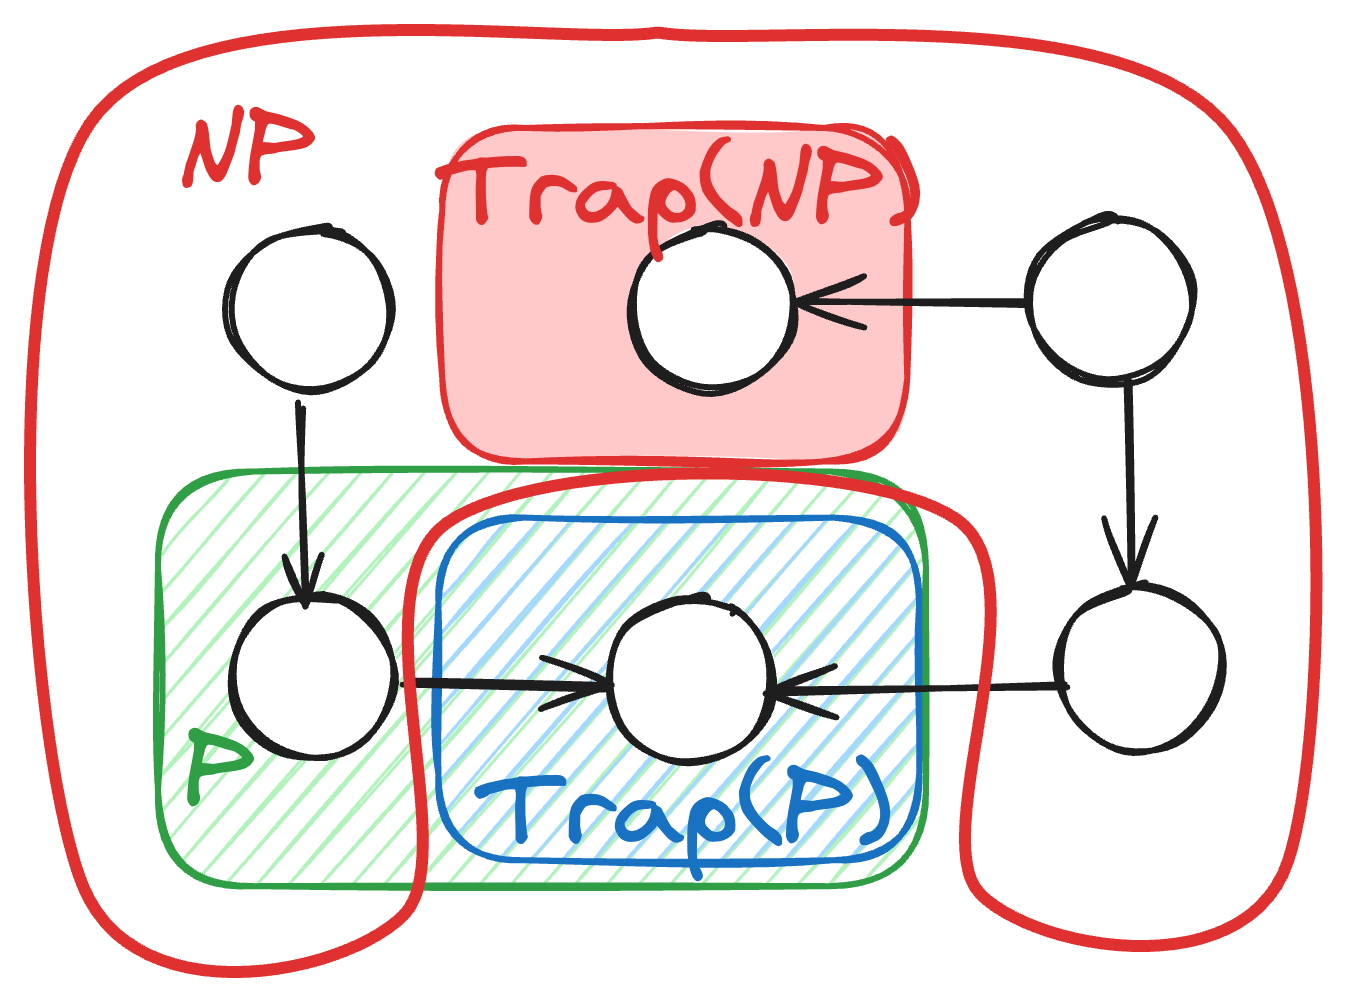
\includegraphics[width=0.45\textwidth]{Figures/algo_exp_a.png}
	\label{subfig:algo_a}
	}
	\hspace*{10pt}
	\subfloat[BN not stabilizing in phenotype $\phenotype$ due to the oscillating phenotype attractor.]{
	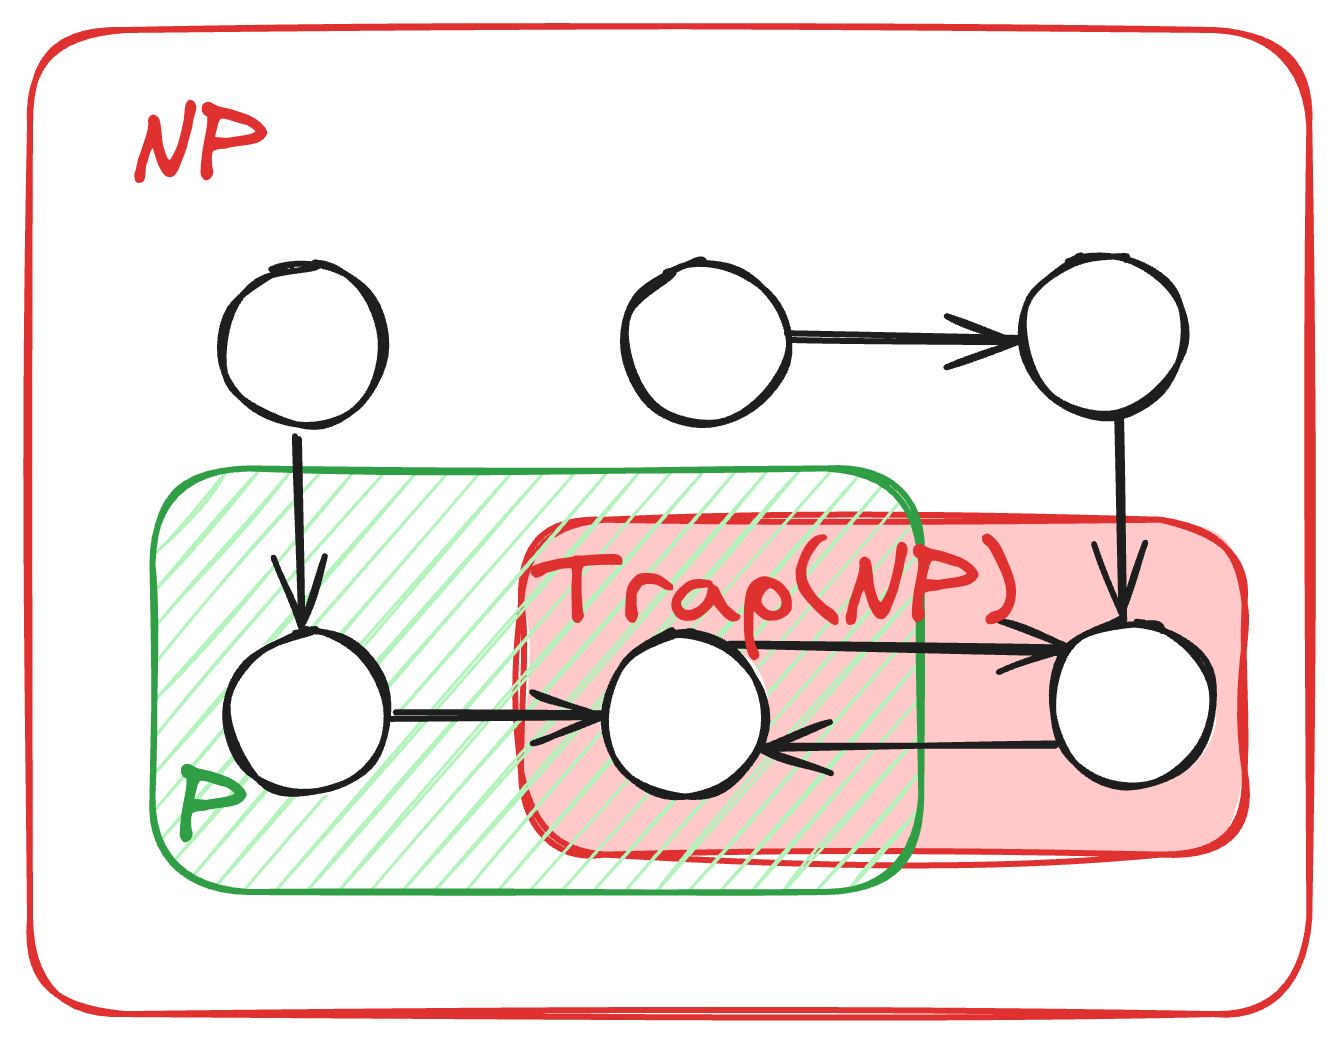
\includegraphics[width=0.45\textwidth]{Figures/algo_exp_b.png}
	\label{subfig:algo_b}
	} \newline
	\subfloat[BN exhibiting oscillating phenotype $\phenotype$ -- computation of $\phenotype$.]{
	\centering
	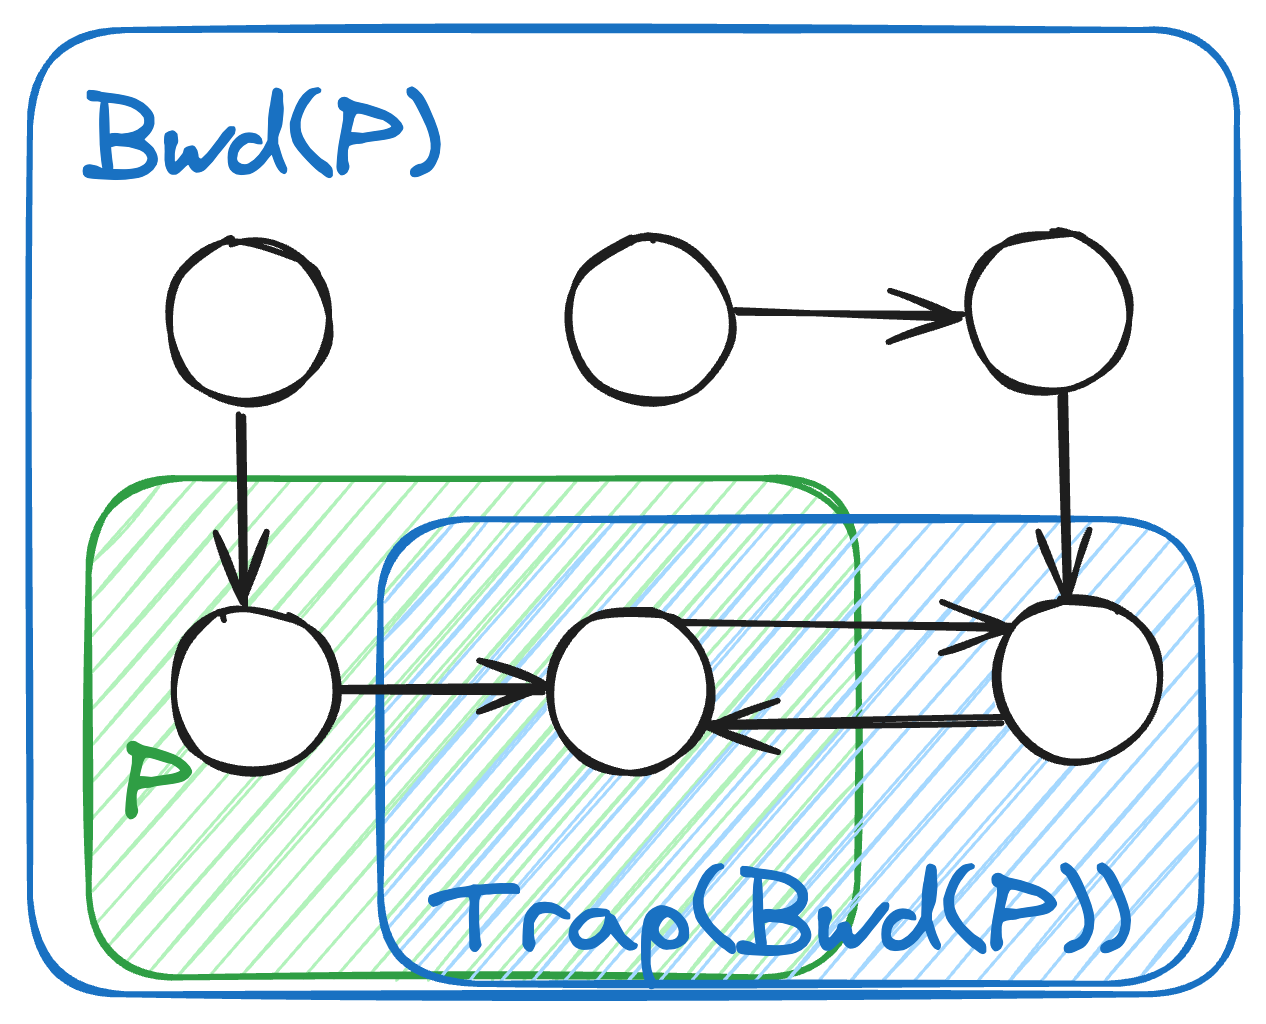
\includegraphics[width=0.45\textwidth]{Figures/algo_exp_c.png}
	\label{subfig:algo_c}
	}
	\hspace*{10pt}
	\subfloat[BN exhibiting oscillating phenotype $\phenotype$ -- computation of $\phenotype' = \vertices \setminus \phenotype$.]{
	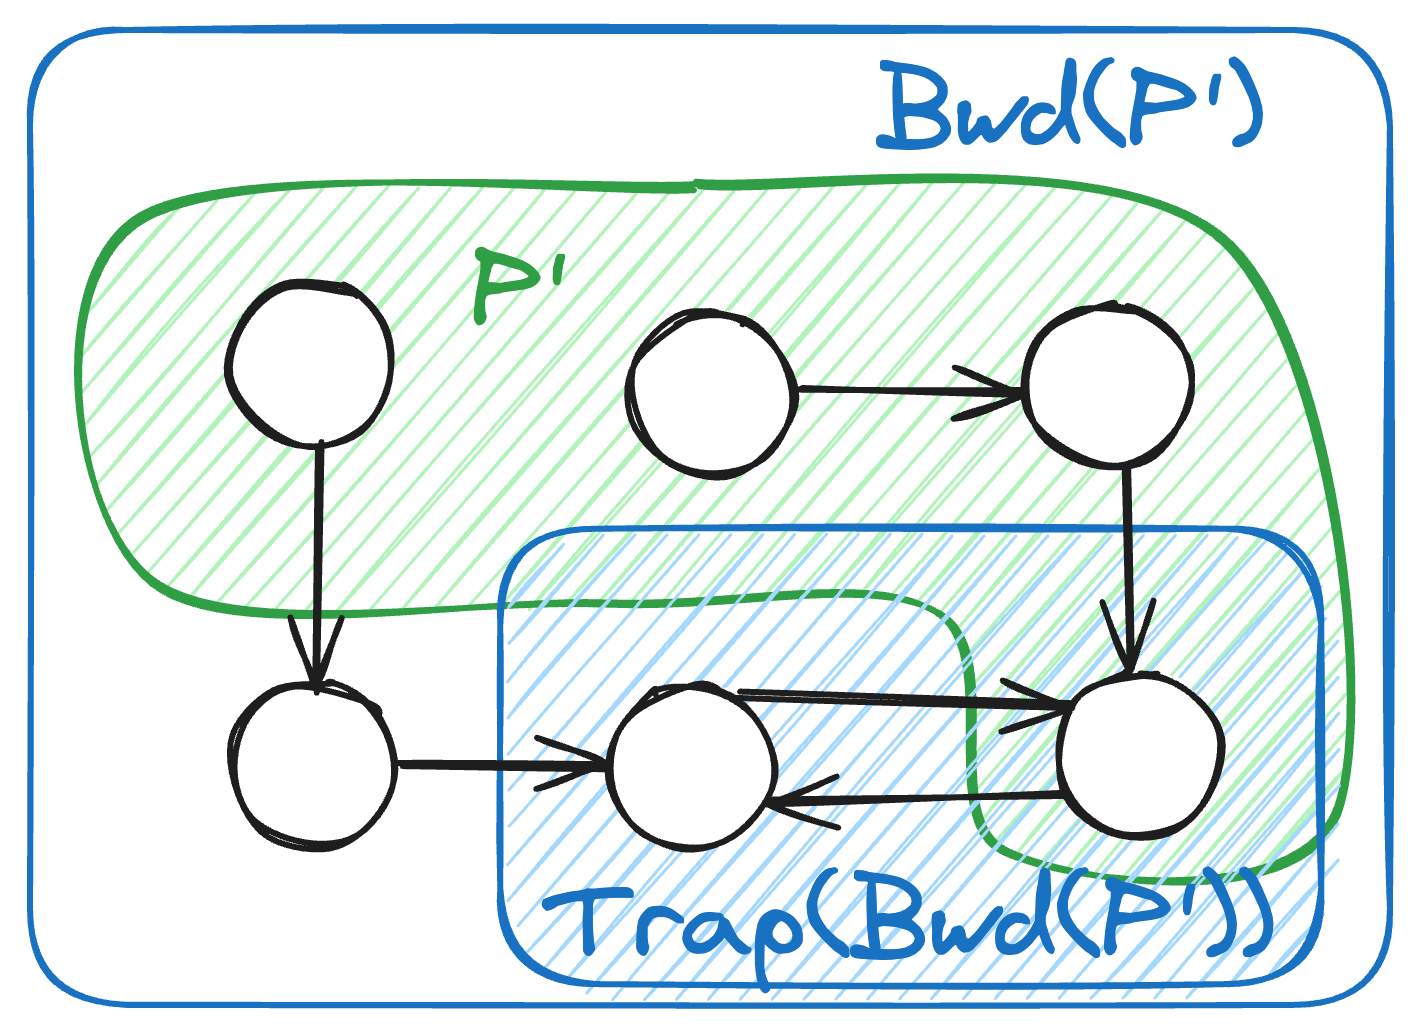
\includegraphics[width=0.45\textwidth]{Figures/algo_exp_d.png}
	\label{subfig:algo_d}
	} \newline
	\subfloat[BN not exhibiting oscillating \phenotype $\phenotype$ -- computation of $\phenotype$.]{
	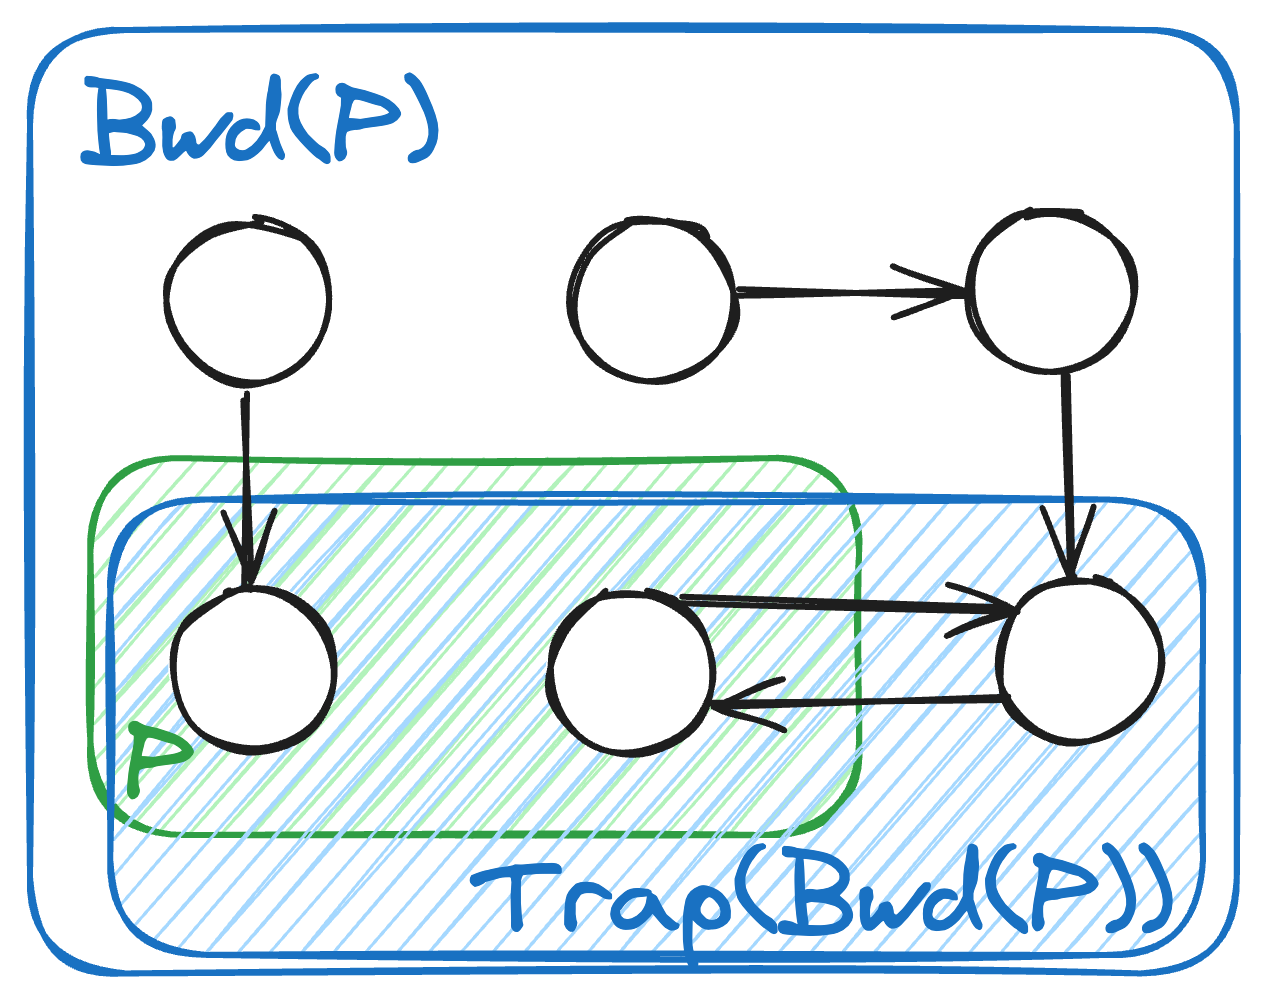
\includegraphics[width=0.45\textwidth]{Figures/algo_exp_e.png}
	\label{subfig:algo_e}
	}
	\hspace*{10pt}
	\subfloat[BN not exhibiting oscillating phenotype $\phenotype$ -- computation of $\phenotype' = \vertices \setminus \phenotype$.]{
	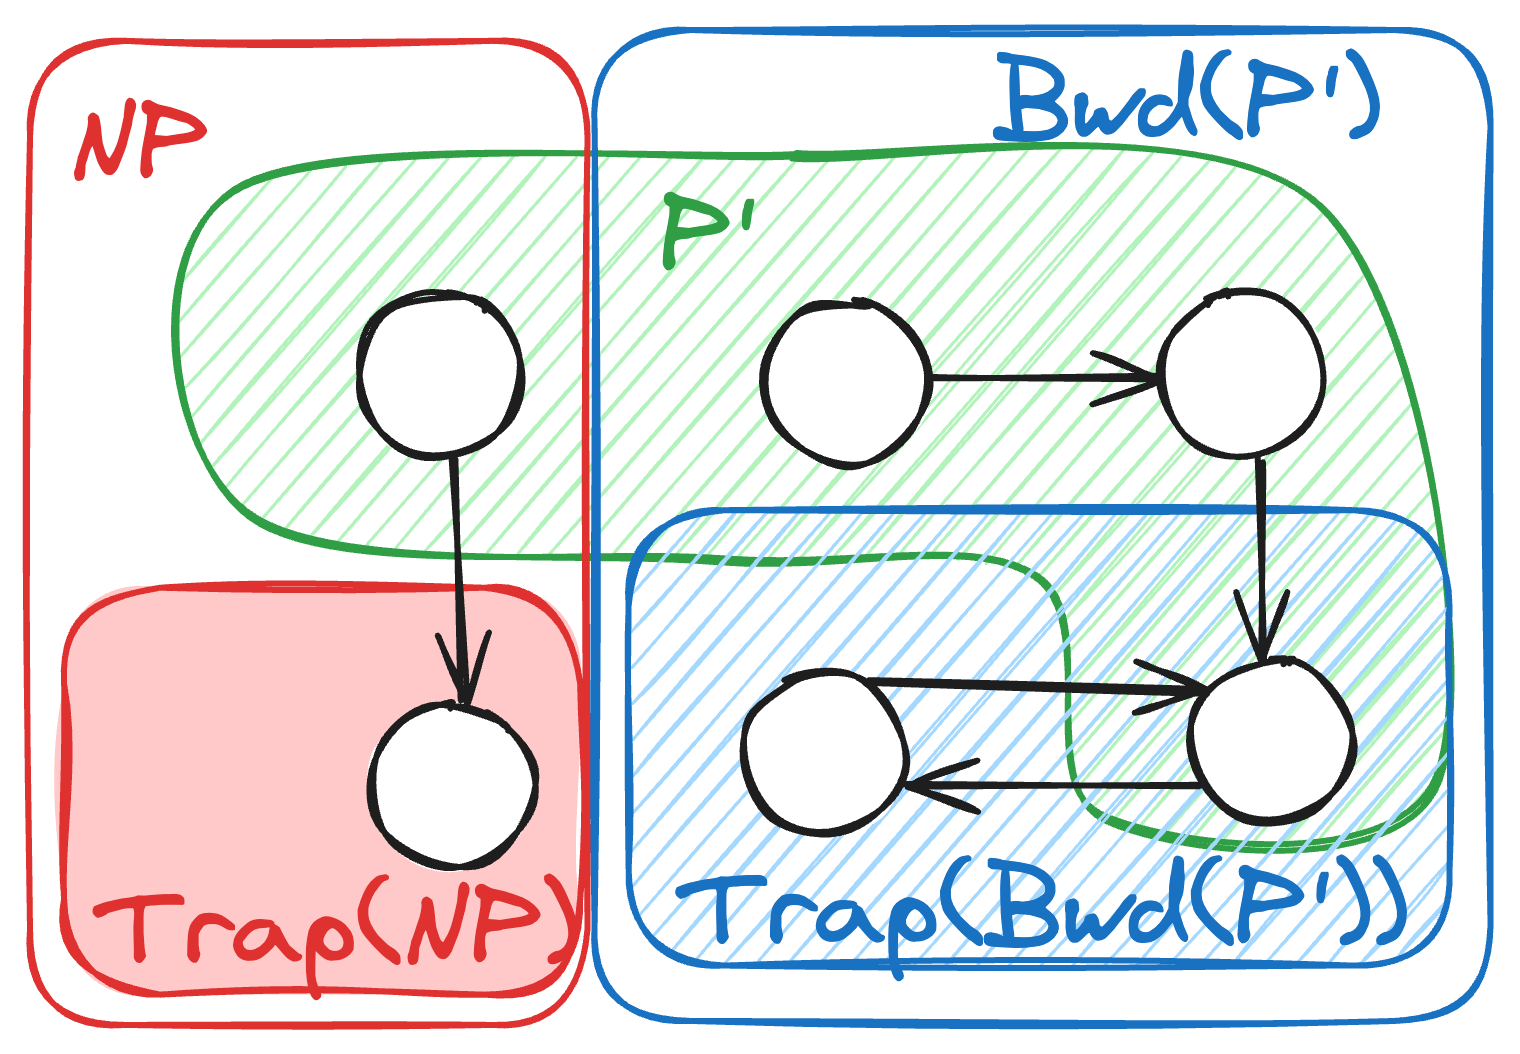
\includegraphics[width=0.45\textwidth]{Figures/algo_exp_f.png}
	\label{subfig:algo_f}
    }
	\caption{\textbf{Examples of \autoref{algo:control} progressions.} \autoref{sub@subfig:algo_a} and \autoref{sub@subfig:algo_b} show situations where BN does not stabilize in the given phenotype considering not allowed oscillation. \autoref{sub@subfig:algo_c} and \autoref{sub@subfig:algo_d} show the computation of the oscillating phenotype $\phenotype$ and its complement $\phenotype'$ for the BN exhibiting the oscillating phenotype. \autoref{sub@subfig:algo_e} and \autoref{sub@subfig:algo_f} show the same computation for the BN not exhibiting the phenotype.}
	\label{fig:algo_highlights}
  \end{figure}
  
  In the case of a non-oscillatory phenotype, we first find the maximal trap set in the phenotype space itself. Thus, we obtain a set of states that contain all attractors stabilizing in the phenotype. We do not need to compute the specific attractors, since it is not necessary for the phenotype control and such a specific attractor refinement might be costly for big networks. After that, we verify, whether remaining reachable space contains any trap set (which would surely contain at least one attractor). If the obtained trap set is empty, that means there are no other attractors than the ones which stabilize in the phenotype, and thus we can say, that the whole network stabilizes the phenotype. The example of an opposite situation can be seen in F\autoref{subfig:algo_a}. Also, as it can be seen from \autoref{subfig:algo_b}, the attractors only oscillating trough $\phenotype$ will be also detected as trap sets negating the phenotype, since they will not be included in $\textsc{Trap}(\phenotype)$.
  
  In order to allow also the oscillatory attractors, we extend the phenotype space by the states that are backward-reachable from the phenotype space. This way, attractors that only oscillate through the phenotype are captured by the trap set as well. Notice, that set $\textsc{Trap}(\textsc{Bwd}(\phenotype))$ cannot contain any attractors completely outside of $\phenotype$ (in $\textsc{Bwd}(\phenotype) \setminus \phenotype$). This is because attractor states, by definition, cannot include any states that are unreachable from themselves. This would contradict the method by which we obtained the set (the backward reachability from the phenotype itself). Therefore, by expanding the considered states for trap set computation, we obtain both - attractors that stabilize in the phenotype and attractors that oscillate through it.
  
  The function \textsc{IsPhenotypeControlAux} can be used as a stand-alone function when either just phenotype-stabilizing or both phenotype-stabilizing and oscillating networks are desired. Also, the phenotype avoidance algorithm is rather trivial, since it is sufficient to reverse the phenotype space as $\phenotype'= \vertices \setminus \phenotype$ and compute the control without allowing oscillation. However, the method \textsc{IsPhenotypeControlAux} on its own cannot guarantee that all attractors in the network are indeed oscillatory towards $\phenotype$.
  
  That is why we also introduce a wrapper function \textsc{IsPhenotypeControl} which exactly supports the defined network-phenotype relationships. The algorithm for phenotype stabilization and avoidance is rather trivial. For oscillatory phenotype also a rather straightforward approach is used -- we verify whether the network doesn't avoid both $\phenotype$ and $\phenotype'= \vertices \setminus \phenotype$ when the oscillation is allowed. These two steps of computation on a network that oscillates through a phenotype are illustrated in \autoref{subfig:algo_c} and \autoref{subfig:algo_d}. On the other hand, \autoref{subfig:algo_e} and \autoref{subfig:algo_f} show a scenario, where the network is not oscillating because of the presence of an attractor stabilizing in $\phenotype$. Notice, that such cases are not possible to detect with a single run of \textsc{IsPhenotypeControlAux}.
  
  In the end, the \textsc{IsPhenotypeControl} is done on all perturbed network instances simultaneously. To do that, we take advantage of our symbolic computational model. Since perturbed instances are expected to have similar STGs, this heuristic approach is expected to be more efficient than computing results on each of the graphs distinctively. The perturbed instances which do not satisfy phenotype control objectives are then discarded. As a result, we obtain a "semi-product", which we need to query, to decode the actual perturbation values and the final results as in \autoref{def:complete_phenotype_control}. The details of this algorithm part can be found in~\cite{Benes2023b}.

\section{Evaluation}
%TODO: Ak bude miesto, tak sa vymedzit voci Fontalnas - my riesime inputy inak

In this section, we evaluate our proposed semi-symbolic method. For the implementation, we use the Rust language and libraries of the AEON tool~\cite{aeon}. This prototype implementation is available as an open-source GitHub repository\footnote{\url{https://github.com/sybila/biodivine-pbn-control/}}. The repository also includes auxiliary scripts we used for the measurements and the raw results. All experiments were performed using a computer with AMD Ryzen Threadripper 2990WX 32-Core Processor and 64GB of memory.

\subsection{Performance}

\paragraph{Benchmark model set} We use real-world Boolean networks to evaluate our method. All tested networks contain input nodes which can be viewed as functionally equivalent to zero-arity uninterpreted functions in PSBNs. We thus treat these inputs as unknown external signal beyond our control. 

\begin{table}[t]
    \caption{Comprehensive overview of the tested real-world Boolean networks. The first four columns contain the model name and the counts of network inputs, all variables, and perturbable variables, respectively. Column $\mathcal{Q}_{\leq3}$ represents the number of all admissible perturbations of size up to three. Sixth column gives a reference to the literature that describes each model. Lastly, the seventh column contains variables that we do not allow to be perturbed.}\label{tab:models}
	\setlength{\tabcolsep}{4pt}
	% \renewcommand{\arraystretch}{1} 
	%\small
	\vspace{10pt}
    \centering
    \begin{tabular}{|l|c|c|c|c|c|p{3.9cm}|}
    \hline
        \textbf{Model} & \textbf{Ins} & \textbf{Vars} & \textbf{Per.} & $\mathcal{Q}_{\leq3}$ & \textbf{Ref.} & \textbf{Uncontrollable vars} \\ \hline
        Cardiac & 2 & 13 & 11 & 6,252 & \cite{Herrmann2012} & $\var{Tbx1}, \var{Tbx5}$ \\ \hline
        Red. MAPK & 4 & 14 & 11 & 25,008 & \cite{Grieco2013} & $\var{Apoptosis}, \var{Growth\_Arrest},$ $ \var{Proliferation}$ \\ \hline
        ERBB & 1 & 19 & 18 & 14,354 & \cite{Ito2012} & $\var{pRB1}$ \\ \hline
        Tumour & 2 & 30 & 24 & 69,380 & \cite{Cohen2015} & $\var{Apoptosis}, \var{Metastasis},$ $ \var{Invasion}, \var{Migration},$ $ \var{EMT}, \var{CellCycleArrest} $ \\ \hline
        Cell Fate & 2 & 31 & 26 & 88,612 & \cite{Calzone2010} & $\var{Apoptosis}, \var{Survival}, $ $ \var{Death}, \var{Division}, \var{NonACD}$ \\ \hline
        Full MAPK & 2 & 49 & 46 & 2,010,768 & \cite{Grieco2013} & $\var{Apoptosis}, \var{Growth\_Arrest},$ $ \var{Proliferation}$ \\ \hline
    \end{tabular}
\end{table}

\autoref{tab:models} lists all models and their relevant characteristics, including number of inputs, variables, perturbable variables, and reference to the original publication. We also state the number of admissible perturbations of size up to three. Previous work shows that such relatively small size is both realistic to implement in practice~\cite{borriello2021,Fontanals2022b,Su2019FM} and robust enough in the presence of partially unknown dynamics~\cite{brim2022}. This number therefore represents how many models would need to be explored in a brute-force based methods for the models of the given size. The table also lists variables which we explicitly do not allow to be perturbed. These variables are mostly outputs and they represent traits which induce individual phenotypes. Therefore, perturbing these variables would lead to trivial control which is neither viable nor interesting.

The first model illustrates cardiac progenitor cells differentiation into the first heart field (FHF) or second heart field (SHF)~\cite{Herrmann2012}. The second and sixth models represent Mitogen-Activated Protein Kinase (MAPK) network representing signalling pathways involved in diverse cellular processes including cancer deregulations. We use both the full and reduced versions of this model as stated in~\cite{Grieco2013}. The third model depicts the key event preceding breast cancer cells proliferation which is the hyper-phosphorylation and subsequent lack of pRB. This process is regulated by ERBB kinase, the lack of which is considered a~breast cancer marker~\cite{Sahin2009}. The fourth model focuses on specific conditions which lead to a metastatic tumour~\cite{Cohen2015}. Finally, the cell fate model provides a high-level understanding of the interplays between pro-survival, necrosis, and apoptosis pathways in response to death receptor-mediated signals~\cite{Calzone2010}.


\begin{table}[t]
\caption{Performance of PSBN control. The first two columns contain model and phenotype names. Then, for perturbations of the size up to three, we list the computation time and maximal robustness found in perturbations of this size. Last column gives the number of minimal perturbations with $\rho = 1.0$.}%
\label{tab:performance}
\setlength{\tabcolsep}{4pt}
% \renewcommand{\arraystretch}{1.1} 
\centering
\vspace{10pt}
\begin{tabular}{|l|l|cc|cc|cc|c|}
\hline
\multirow{2}{*}{Model}     & \multirow{2}{*}{Phenotype} & \multicolumn{2}{c|}{Size 1}  & \multicolumn{2}{c|}{Size 2} & \multicolumn{2}{c|}{Size 3} & {\# Min. per.} \\
\cline{3-8}
                           &                            & \MC{Time}  & $\rho$          & \MC{Time}  & $\rho$         & \MC{Time}      & $\rho$     & {($\rho=1.0$)} \\
\hline
\multirow{3}{*}{Cardiac}   & FHF                        & \MC{$<$1s} & 0.5             & \MC{$<$1s} & 1.0            & \MC{$<$1s}     & 1.0        & 4       \\
                           & SHF                        & \MC{$<$1s} & 0.5             & \MC{$<$1s} & 1.0            & \MC{$<$1s}     & 1.0        & 2       \\
                           & No mesoderm                & \MC{$<$1s} & 0.5             & \MC{$<$1s} & 1.0            & \MC{$<$1s}     & 1.0        & 3       \\
\hline
\multirow{4}{*}{Red. MAPK} & Apoptosis                  & \MC{$<$1s} & 1.0             & \MC{$<$1s} & 1.0            & \MC{$<$1s}     & 1.0        & 1       \\
                           & Growth arrest              & \MC{$<$1s} & 0.75            & \MC{$<$1s} & 1.0            & \MC{$<$1s}     & 1.0        & 1       \\
                           & No decision                & \MC{$<$1s} & 1.0             & \MC{$<$1s} & 1.0            & \MC{$<$1s}     & 1.0        & 1       \\
                           & Proliferation              & \MC{$<$1s} & 0.25            & \MC{$<$1s} & 1.0            & \MC{$<$1s}     & 1.0        & 3       \\
\hline
\multirow{2}{*}{ERBB}      & Phosphor.                  & \MC{$<$1s} & 1.0             & \MC{$<$1s} & 1.0            & \MC{$<$1s}     & 1.0        & 7       \\
                           & Non-phospor.               & \MC{$<$1s} & 1.0             & \MC{$<$1s} & 1.0            & \MC{$<$1s}     & 1.0        & 8       \\
\hline
\multirow{4}{*}{Tumour}    & Apoptosis                  & \MC{2s}    & 1.0             & \MC{8s}    & 1.0            & \MC{23s}       & 1.0        & 2       \\
                           & EMT                        & \MC{$<$1s} & 0.5             & \MC{3s}    & 1.0            & \MC{11s}       & 1.0        & 15      \\
                           & Hybrid                     & \MC{$<$1s} & 0.25            & \MC{5s}    & 1.0            & \MC{24s}       & 1.0        & 3       \\
                           & Metastasis                 & \MC{$<$1s} & 0.5             & \MC{$<$1s} & 1.0            & \MC{1s}        & 1.0        & 6       \\
\hline
\multirow{4}{*}{Cell Fate} & Apoptosis                  & \MC{$<$1s} & 0               & \MC{4s}    & 1.0            & \MC{58s}       & 1.0        & 24      \\
                           & Naive                      & \MC{$<$1s} & 0               & \MC{2s}    & 1.0            & \MC{29s}       & 1.0        & 8       \\
                           & Necrosis                   & \MC{$<$1s} & 1.0             & \MC{$<$1s} & 1.0            & \MC{11s}       & 1.0        & 1       \\
                           & Survival                   & \MC{$<$1s} & 1.0             & \MC{2s}    & 1.0            & \MC{21s}       & 1.0        & 1       \\
\hline
\multirow{4}{*}{Full MAPK} & Apoptosis                  & \MC{$<$1s} & 1.0             & \MC{7s}    & 1.0            & \MC{14min}     & 1.0        & 6       \\
                           & Growth arrest              & \MC{4s}    & 0.75            & \MC{4s}    & 1.0            & \MC{22min}     & 1.0        & 47      \\
                           & No decision                & \MC{3s}    & 0.81            & \MC{107s}  & 1.0            & \MC{22min}     & 1.0        & 45      \\
                           & Proliferation              & \MC{3s}    & 0.25            & \MC{3s}    & 1.0            & \MC{20min}     & 1.0        & 8       \\
\hline                
\end{tabular}
\end{table}



\paragraph{Performance evaluation on real-world models} In \autoref{tab:performance}, we show results of computing phenotype control on all our benchmark models from \autoref{tab:models}. We use real-world phenotypes as described in the source literature. These are typically subspaces obtained by fixing network outputs to the desired values. The details of exact phenotypes can be found in the git repository. 

For each model and its phenotype, we computed all working perturbations of size up to three. We then show the times needed for individual computations (including enumeration and robustness calculation), the highest robustness achieved for each case, and the number of minimal perturbations with 100\% robustness.

\begin{table}[!ht]
\caption{Minimal perturbations for reduced MAPK model. The first column is target phenotype while other columns contain minimal perturbations for unperturbed model, model with over-expressed \var{EGFR}, and model with \var{FGFR3} gain-of-function. Variables divided by $/$ stand for perturbing either of them. $\emptyset$ is used when no perturbation is necessary.}%
\label{tab:red_mapk}
% \setlength{\tabcolsep}{4pt}
% \renewcommand{\arraystretch}{1} 
%\footnotesize
\centering
\vspace{10pt}
\begin{tabular}{|c|p{3.4cm}|p{3.4cm}|p{3.4cm}|}
\hline
\textbf{Phenot.} & \textbf{Unperturbed} & \textbf{Perturbed} $\var{EGFR}{\shorteq}1$ & \textbf{Perturbed} $\var{FGFR3}{\shorteq}1$ \\ \hline
Apoptosis & $\var{DNA\_dmg}{\shorteq}1,\var{TGFBR\_st}{\shorteq}1,$ $\var{FRS2}{\shorteq}1$ & $\textcolor{OliveGreen}{\var{DNA\_dmg}{\shorteq}1},\textcolor{OliveGreen}{\var{TGFBR\_st}{\shorteq}1},$ $\var{ERK}{\shorteq}0,\var{p53}{\shorteq}1$ & $\textcolor{OliveGreen}{\var{DNA\_dmg}{\shorteq}1},\textcolor{OliveGreen}{\var{TGFBR\_st}{\shorteq}1},$ $\var{ERK}{\shorteq}0,\var{p53}{\shorteq}1$ \\ \hline
$\neg$Apoptosis & $\emptyset$ & $\textcolor{OliveGreen}{\var{AKT}{\shorteq}1},\var{ERK}{\shorteq}1,\var{MSK}{\shorteq}0,$ $\textcolor{OliveGreen}{\var{PTEN}{\shorteq}0},\textcolor{OliveGreen}{\var{p14}{\shorteq}0},\textcolor{OliveGreen}{\var{p53}{\shorteq}0}$ & $\textcolor{OliveGreen}{\var{AKT}{\shorteq}1},\var{ERK}{\shorteq}1,\var{MSK}{\shorteq}0,$ $\textcolor{OliveGreen}{\var{PTEN}{\shorteq}0},\textcolor{OliveGreen}{\var{p14}{\shorteq}0},\textcolor{OliveGreen}{\var{p53}{\shorteq}0}$ \\ \hline
Prolif. & $\var{ERK}{\shorteq}1$ & $\textcolor{OliveGreen}{\var{p14}{\shorteq}0},$ $\textcolor{OliveGreen}{\var{p53}{\shorteq}0}$& $\{\var{p14}/\var{p53}{\shorteq}0,\var{FRS2}{\shorteq}1\},$ $\{\var{p14}/\var{p53}{\shorteq}0,\var{PI3K}{\shorteq}1\},$ $\{\var{p14}/\var{p53}{\shorteq}0,\var{EGFR}{\shorteq}1\}$ \\ \hline
$\neg$Prolif. & $\emptyset$& $\textcolor{OliveGreen}{\var{DNA\_dmg}{\shorteq}1},\textcolor{OliveGreen}{\var{TGFBR\_st}{\shorteq}1},$ $\var{AKT}{\shorteq}0,\var{ERK}{\shorteq}0,\var{MSK}{\shorteq}0,$ $\var{PI3K}{\shorteq}0,\var{PTEN}{\shorteq}1,\var{p53}{\shorteq}1$& $\textcolor{OliveGreen}{\var{DNA\_dmg}{\shorteq}1},\textcolor{OliveGreen}{\var{TGFBR\_st}{\shorteq}1},$ $\var{AKT}{\shorteq}0,\var{ERK}{\shorteq}0,\var{MSK}{\shorteq}0,$ $\var{PI3K}{\shorteq}0,\var{PTEN}{\shorteq}1,\var{p53}{\shorteq}1$ \\ \hline
No decis. &  $\emptyset$ & $\var{MSK}{\shorteq}0$& $\var{MSK}{\shorteq}0$ \\ \hline
$\neg$No decis. & $\var{DNA\_dmg}{\shorteq}1, \var{TGFBR\_st}{\shorteq}1$ $\var{EGFR}{\shorteq}1,$ $\var{ERK}{\shorteq}1,$ $\var{FRS2}{\shorteq}1,$ $\var{p53}{\shorteq}1$& $\textcolor{OliveGreen}{\emptyset}$ & $\var{DNA\_dmg}{\shorteq}1,\var{TGFBR\_st}{\shorteq}1$ $\var{ERK}{\shorteq}1,\var{FRS2}{\shorteq}1,\var{p53}{\shorteq}1,$ $\var{PI3K}{\shorteq}1$  \\ \hline    
\end{tabular}
\end{table}

The performance of our method is almost instant for small-sized models which is very convenient for practical use. As for the bigger models, the method also performs sufficiently, nonetheless, due to complex unpredictable nature of PSBN dynamics, its performance may vary significantly from case to case. For example, even though Cell Fate model has only one more perturbable variable than the Tumour model, we can notice that perturbations of size three take on average twice longer to compute. The differences in PSBN dynamics can also have big impact within the same model for different phenotypes. Even though the phenotypes within the same model are all of the same size, we can notice that in any of the bigger models and perturbations of size three, the control takes much longer to compute. There are many factors which can contribute to these big performance differences such as fixed-point nature of the trap set algorithm (which might require numerous iterations in case of long paths with few neighbors) or heuristic BDD representation.


% TODO: pseudoporovnanie sa s brute-force? -> asi nie, vychadza to divne, je tazke ferovo urcit vypoctovy cas na 1 instance 

% Finally, we must also factor for the enumeration of possible perturbations and respective colours working for these perturbations. Again, due to heuristic BDD mechanics and unpredictable final results (i.e., number of working perturbations), it is not really possible to make good estimates of the final duration of this operation. Nonetheless, the resulting computational time is still within practically usable time frames. Here, we state how long this enumeration lasts for all possible perturbations with size up to three (the worst case for our setting), nonetheless, the enumeration could be terminated also earlier; for example, either after first working perturbation or after enumerating all working perturbations with minimal size. Any of these approaches would result into significantly shorter times for this part of computation.


% Please add the following required packages to your document preamble:
% \usepackage{multirow}


\chapter{Software}
\label{chapter:software}

In this chapter, we describe the technical details of the software tools we developed for the control of Boolean networks. We first give an overview of the software. Then we describe the implementation underlying backend details of the main components of the software. Finally, we describe the python package and the web application that we developed to make the software accessible to a wider audience.

\section{Software overview}
\label{sec:software_architecture}

The software for the control of \PBN{} networks was developed as part of the BioDivine tools\footnote{\url{https://sybila.fi.muni.cz/tools.html}} developed by the Sybila~\footnote{\url{https://sybila.fi.muni.cz/index.html}} (Systems Biology Laboratory) research group at Masaryk University. 

The tools were initially oriented on a ``colored model checking'' of parametrized continuous models of biological systems~\cite{Brim2015}. The approach was also later extended to hybrid models~\cite{Smijakova2020}. The main idea behind colored model checking was encoding the continuous models as discrete color-labelled transition systems, and then applying SMT model checking techniques to analyze their behavior. This approach also enabled solving the parameter synthesis and attractor bifurcation problems for these models~\cite{Benes2016,Benes2017}.

Building on top of the previous work, the group shifted focus from discretized continuous models to Boolean networks, which are a more direct ``natively'' discrete modeling formalism. The former parameters of continuous models and their paramters synthesis was reoriented from continuous values of parameters to unknown functions of the network structure.

At first, the tools were mostly focused on the bifurcation analysis of \PBN{}~\cite{Benes2019}. To nurture the adoption of the tool, a web application was developed to make the tool accessible to a wider audience~\cite{aeon}. The web application allowed users to upload their own partially specified Boolean network models, adjust them and run the bifurcation analysis. 

Since globally there was not a lot of tools supporting analysis of \PBN{} models, the Aeon tools were extended to support also other types of analysis. In particular, we implemented the control of \PBN{} models, which is the main topic of this thesis. The control of \PBN{} models was implemented as a new component of the software, and it was integrated into the web application as well. 

Later, to make the control of \PBN{} models more accessible to users who prefer working with code, we also implemented a python package that provides an interface to the control algorithms implemented in the software~\cite{aeonpy}. The tool also provides all underlying algorithms and data structures such as the symbolic representation of the state space, and the algorithms for computing the attractors and their basins of attraction. The tool is also being extended by higher-level algorithms for the analysis of \PBN{} models, such model checking of temporal properties, and the analysis of the structure of the state space~\cite{Benes2023,Benes2024bnclassifier}.

\begin{figure}[htbp]
    \centering
    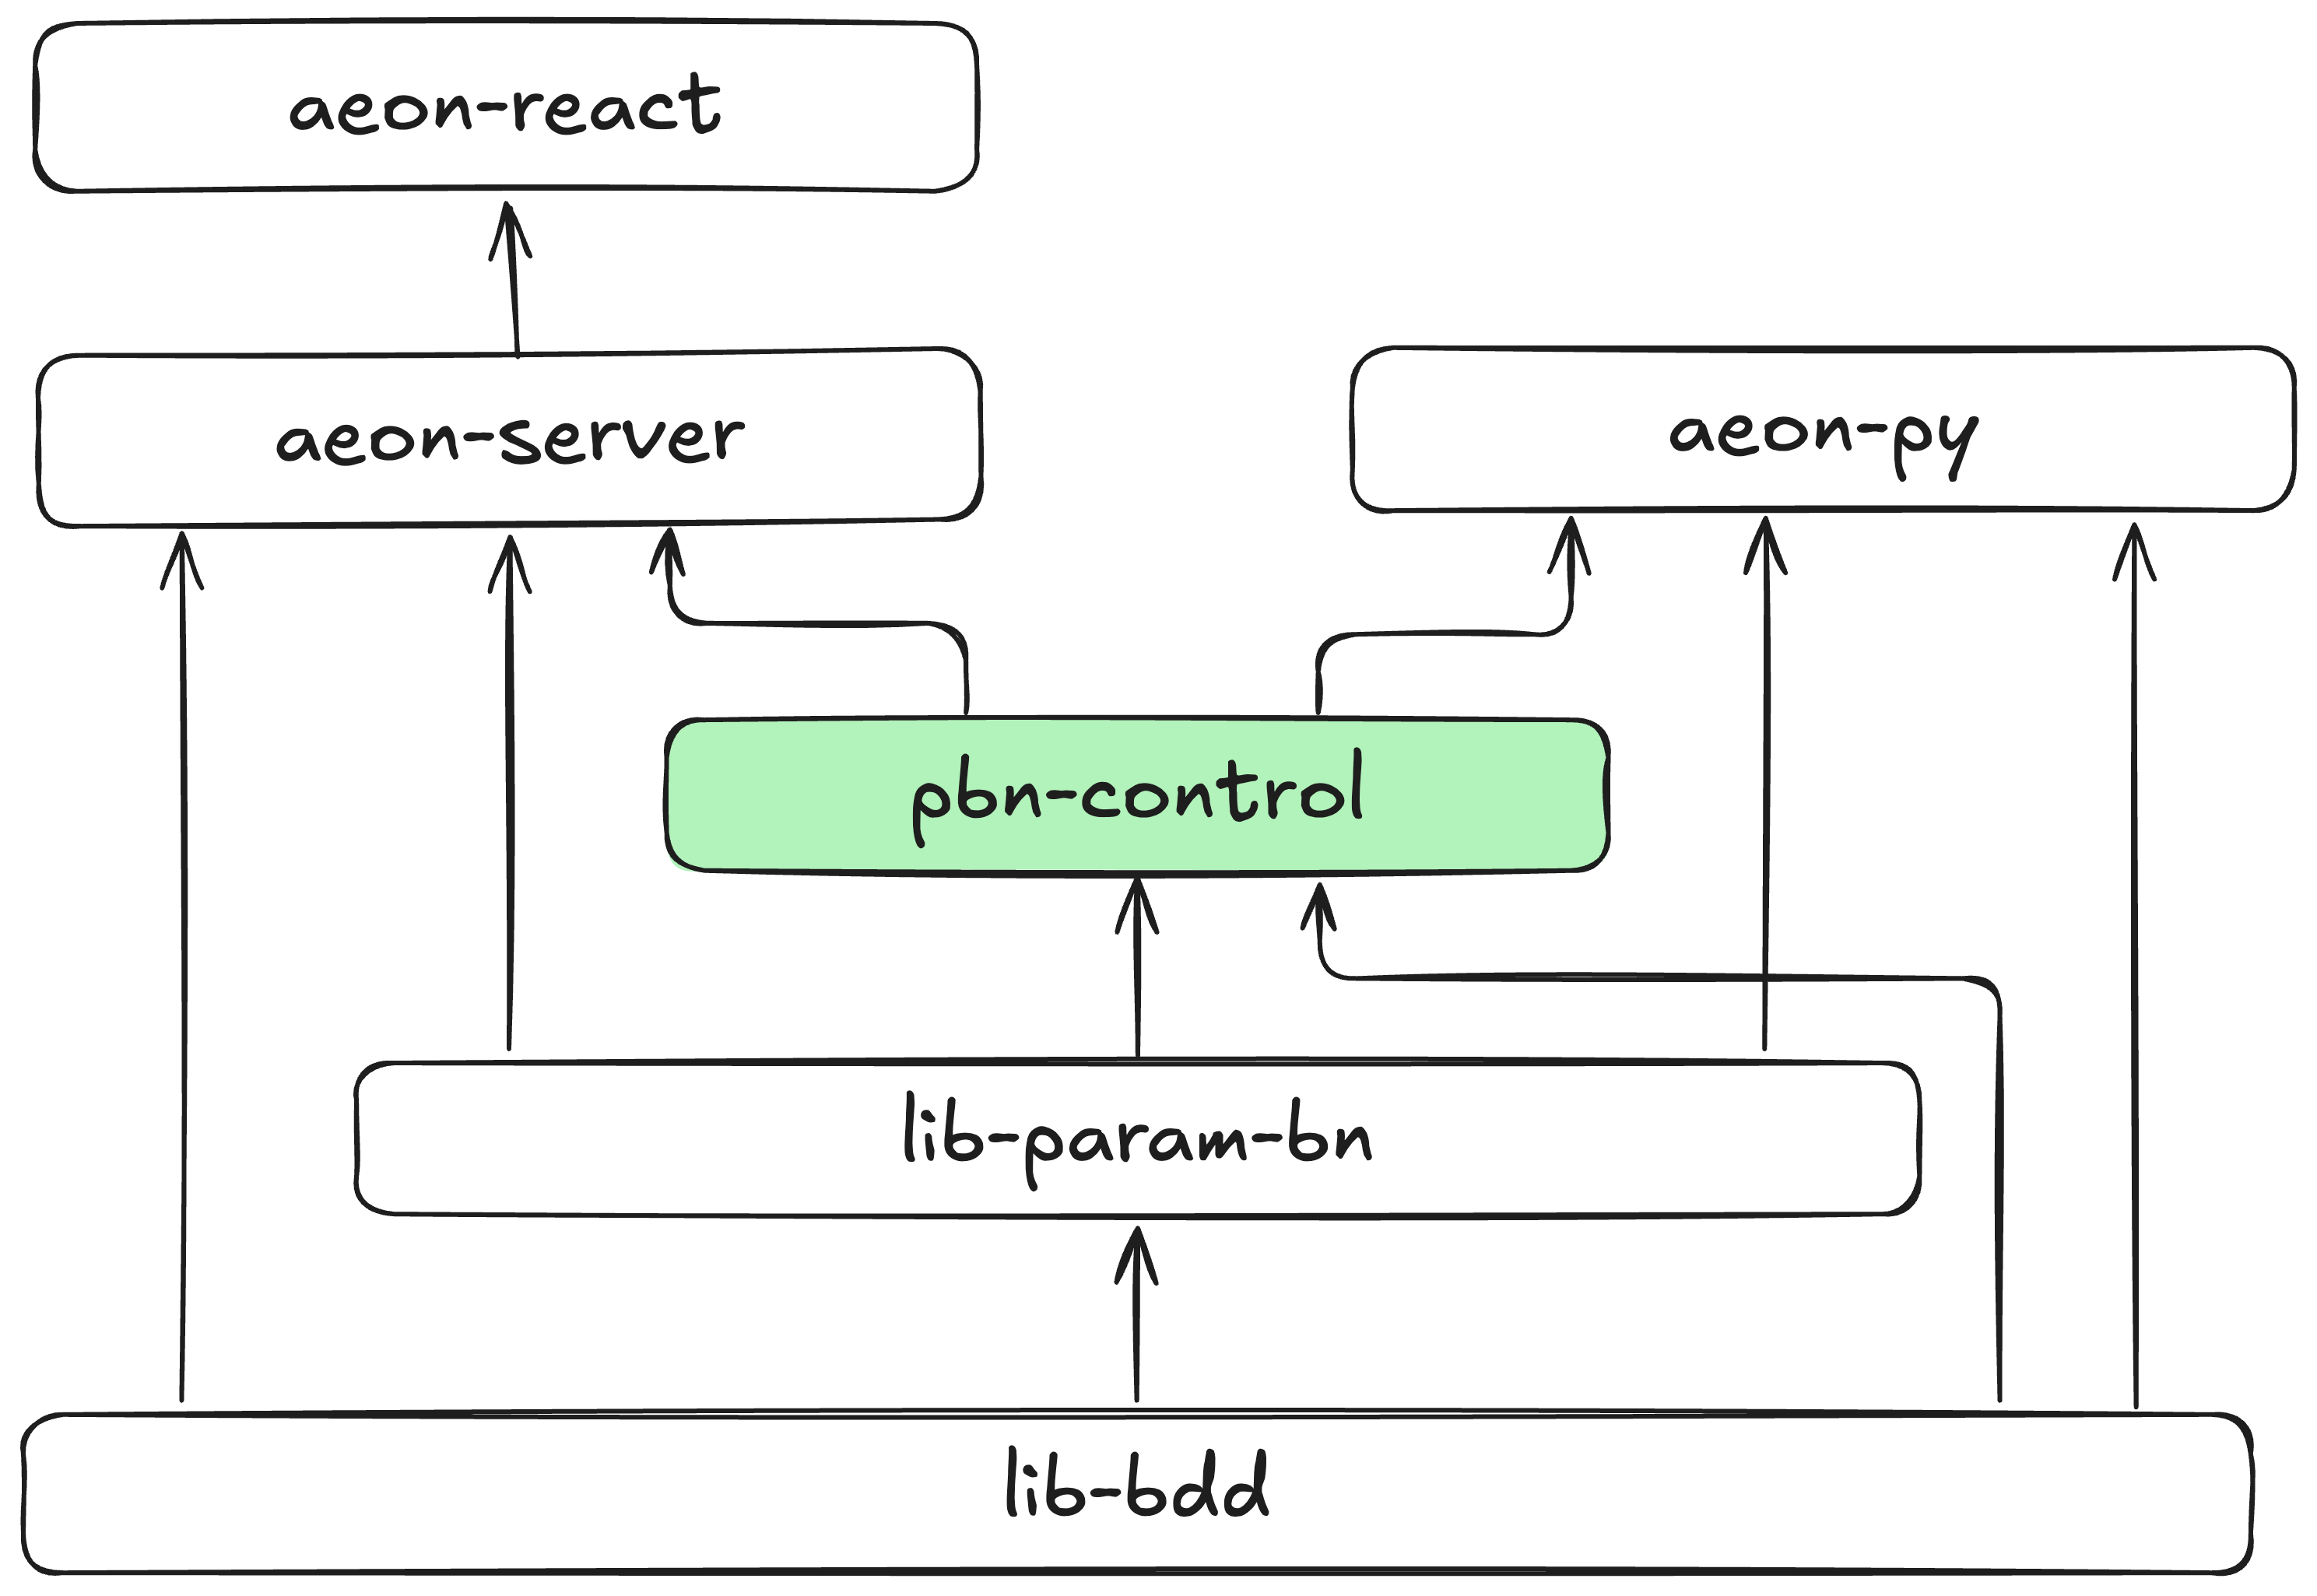
\includegraphics[width=0.8\textwidth]{Figures/sw_arch.png}
    \caption{
        \textbf{Biodivine Aeon software architecture overview.} The figure depicts components of the biodivine software related to the control of Boolean networks. The green box represents the main Rust library, which contains the core algorithms and data structures for Boolean network control. The arrows indicate the dependencies between the components. 
    }
    \label{fig:sw_arch}
\end{figure}

In \autoref{fig:sw_arch}, we give an overview of the software architecture of the Aeon tools. The core components are implemented in Rust language because of its performance, memory safety and mature developer experience. Component lib-bdd is the low-level library for the symbolic representation of the state space using binary decision diagrams (BDDs). It is independent of Boolean networks and can be used for any application that requires symbolic representation of state spaces. 

Component lib-param-bn is the main library for the performant analysis of \PBN{} models, which contains the algorithms for computing attractors, reachability algorithms and bifurcation. On top of the two libraries, we implemented the control of \PBN{} models as a new component of the software. Since the control of \PBN{} requires custom encoding of the perturbations it also relies on the lib-bdd library for the symbolic representation of the state space. The control component also relies on the lib-pbn library for computing the attractors and their basins of attraction, which are used in the control algorithms.

Finally, we implemented a web application that is built on top of all the rust components. Aeon-server provides a server functionality such as validation of the uploaded models and progress reporting to interact with the software through a web interface. The web application (aeon-react) than uses just the server component of the software, which provides an API for the users to interact with the software through the web interface. Later, also a python package aeon-py was implemented to provide a convenient python interface for all low-level algorithms and data structures. 

\section{Core packages}
\label{sec:core_packages}

\paragraph{lib-bdd} The lib-bdd library provides a symbolic representation of the state space using binary decision diagrams (BDDs). It provides basic operations for manipulating BDDs, such as conjunction, disjunction, negation, and quantification. 

Compared to many other implementations, each Binary Decision Diagram (BDD) instance manages its own memory. This design simplifies serialization and enables safe sharing between threads, which is particularly beneficial for applications that process large numbers of BDDs concurrently. It also aligns well with the ownership and safety principles emphasized in the Rust programming language.

The implementation provides support for a range of common operations on BDDs. These include standard logical operations, evaluation of Boolean expressions, and transformations between BDD representations and conjunctive or disjunctive normal forms. Additional functionality allows inspection of BDD structures, conversion back to Boolean expressions, and visualization through graph exports. The system also supports several relational-style operations commonly used in symbolic computation, such as projection and restriction. Note that these operations were used in \autoref{subsec:symbolic_ops} and \autoref{sec:phen_control_method} for the control of \PBN{} models.

\paragraph{lib-param-bn} The lib-param-bn library is the main library for the performant analysis of \PBN{} models, which contains the algorithms for computing attractors, reachability algorithms and bifurcation. In particular, it implements fully \emph{symbolic} representation of the state space of \PBN{} models using BDDs, that can combine interpretations and states in a single BDD. 

This library was used to provide all reachability, trap set and attractor computations for the control algorithms implemented in this thesis that are described in \autoref{subsec:supporting_algos} and \autoref{sec:phen_ctrl_algo}.

Previously the library used semi-symbolic representation of the state space, where only interpretations were represented symbolically, while states were represented explicitly. This approach was used in the initial version of the control algorithms implemented in this thesis, which are described in \autoref{ss:semi_symbolic_sb}.

\paragraph{pbn-control} The pbn-control library provides the necessary functionality for the control of \PBN{} models, including the implementation of various control strategies and algorithms.

In particular, it implements the encoding of perturbations as function symbols (parameters), that are added to the original \PBN{} model. This allows us to use the same symbolic representation of the state space for both the original model and the perturbations, which is crucial for the performance of the control algorithms. The library also implements the algorithms for computing the control and manipulating with the control map relations, which are used in the control algorithms described in \autoref{ss:control_algos_st_otp} and \autoref{sec:phen_ctrl_algo}.

Since we have shown, that symbolic one-step control is superior to semi-symbolic one-step control, the current version of the control algorithms implemented in the software relies on the fully symbolic representation of the state space provided by the lib-param-bn library. However, the initial version of the control algorithms implemented in this thesis, which are described in \autoref{ss:semi_symbolic_sb}, relied on the former semi-symbolic representation of the state space.

\section{Aeon web application}
\label{sec:aeon_web_app}

Aeon web application is a web-based interface for the analysis of \PBN{} models. It allows users to upload their own models, adjust them and run various analyses, including the control of \PBN{} models. The initial version of the web application was developed to make the bifurcation analysis of \PBN{} models accessible to a wider audience. The initial version was first released in 2020~\cite{aeon}. 

In version 0.5.0 of the web application, we integrated the control of \PBN{} models as a new component of the software~\cite{Vesely2025}. During implementation of the new control module, it was discovered, that technical debt in the codebase of the web application was making it difficult to implement the new control module. Therefore, it was decided to refactor the web application to make it more modular and maintainable. This has led to a major refactor of the web application, which was released in version 0.6.0 and which is also briefly presented here.

\begin{figure}[htbp]
    \label{fig:sw_load_model}
    \centering
    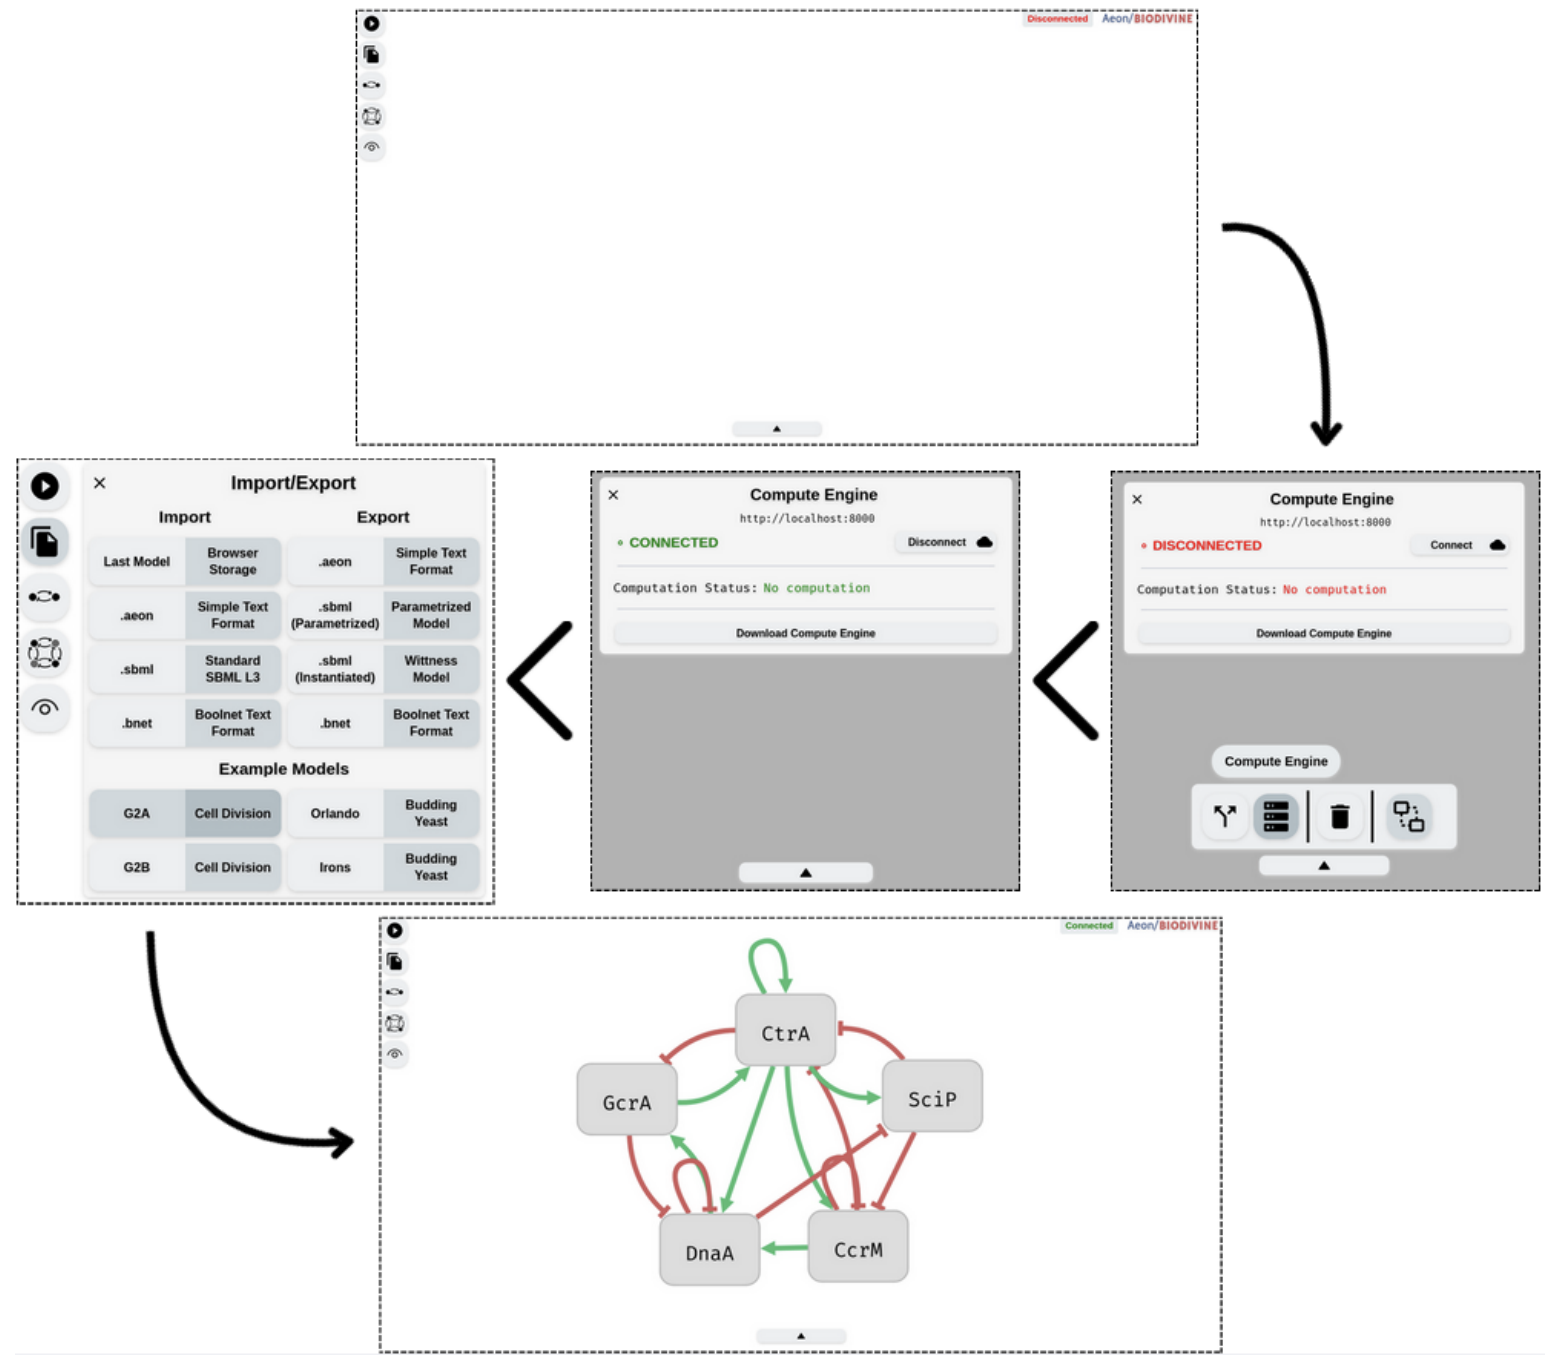
\includegraphics[width=\textwidth]{Figures/aeon_load_model.png}
    \caption{
        \textbf{Biodivine Aeon web application interface.} From~\cite{Vesely2026}. The figure shows the main interface of the Aeon web application, where users can upload and load their own \PBN{}.
    }
\end{figure}

AEON tool is available at \url{https://biodivine.fi.muni.cz/aeon/} as an online tool. Due to the potential high computational complexity of the analyses, SyBiLa group does not provide a public instance of the web application server, but instead provides a downloadable version of the server that users can run on their own machines.

The main flow of how a model can be uploaded and analyzed in the web application is shown in \autoref{fig:sw_load_model}. The user first needs to download and run the server component of the software on their own machine. Then, they can access the web application functionality through a web browser. The user can upload their own \PBN{} model in the form of a text file, which is then validated by the server or select one of the example models provided by the web application. Once the model is loaded, the user can adjust the model by changing the model functions, or by changing the regulations of the model.


\begin{figure}[htbp]
    \centering
    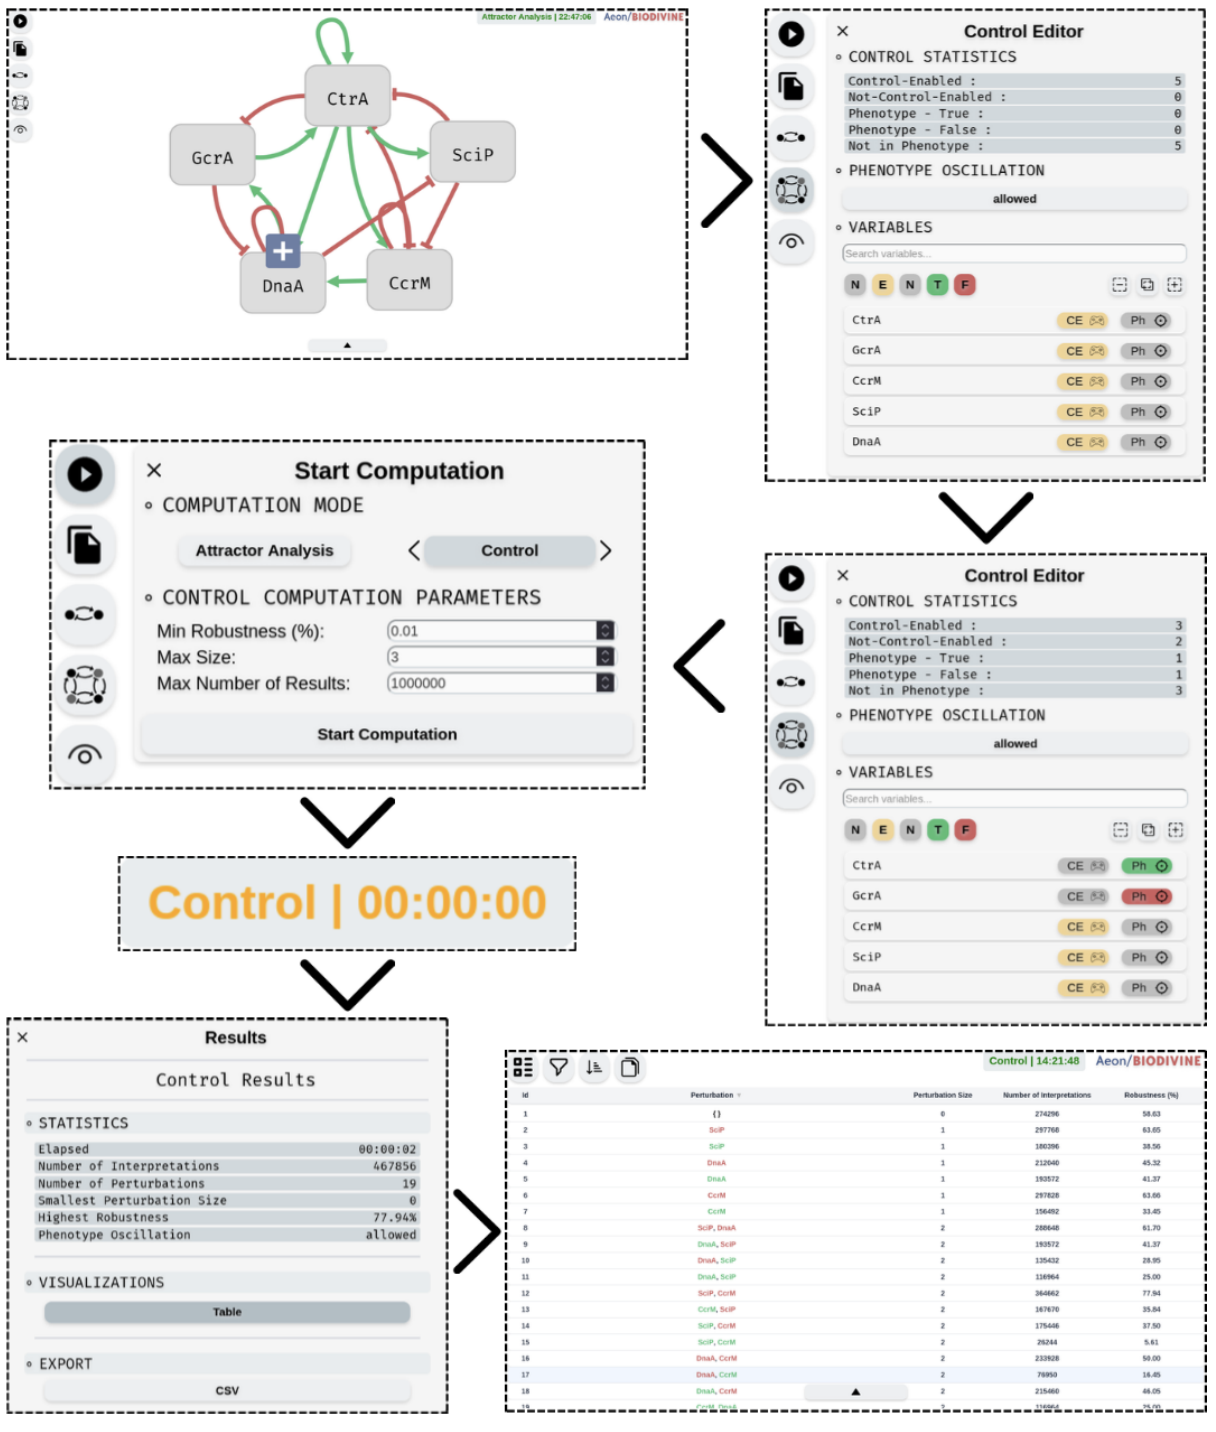
\includegraphics[width=\textwidth]{Figures/aeon_control.png}
    \caption{
        \textbf{Biodivine Aeon web application control interface.} From~\cite{Vesely2026}. The figure shows the control interface of the Aeon web application, where users can control their own \PBN{}.
    }
    \label{fig:sw_control}
\end{figure}


After the model is loaded, the user can run various analyses on the model, including the permanent phenotype control of \PBN{} models. The source-target control is not support via Aeon UI. It could be implemented later if there is a user interest. The control interface of the web application is shown in \autoref{fig:sw_control}. The user can select variables that can be perturbed, the type of the phenotype control (allowed, required or forbidden oscillation) and the target phenotype that they want to reach. The user can also adjust the parameters of the control algorithm, such as the minimal required robustness, maximum number of perturbations allowed or maximum number of results. 

After the control algorithm is run, the results are displayed in the web application, where the user can inspect the results and download in a CSV format for further analysis. The results include the comprehensive statistics about the control problem, such as elapsed time, number of interpretations that can be controlled, the number of perturbations found, highest robustness achieved, and other relevant information. Moreover, a full list of all possible perturbations that can be applied to reach the target phenotype is also available. The list can be filtered and sorted by various criteria, such as the number of perturbations, the robustness of the perturbation, or the variables that are perturbed. 

\section{Aeon.py}
\label{sec:python_package}

Since it can be difficult to develop a web application that covers all the functionality of the a very technical software, we also implemented a python package that provides an interface to the control algorithms implemented in the software~\cite{aeonpy}. The python package is available on PyPI and as part of the CoLoMoTo docker image~\cite{Naldi2015}. 

The CoLoMoTo toolset provides a robust and reproducible computational framework for the analysis of Boolean networks, enabling both qualitative and formal investigation of complex biological regulatory systems. Its Jupyter environment based on Docker ensures interoperability and reproducibility while facilitating scalable exploration of state-space dynamics under different updating schemes. Since it is widely used in the community of Boolean network modeling, we decided to make the Aeon control algorithms available as part of the CoLoMoTo docker image. This allows users who are already using the CoLoMoTo toolset to easily integrate the control algorithms into their existing workflows.

The python package provides a convenient interface for users who prefer working with code rather than a web application. It allows users to load their own \PBN{} models, adjust them and run the control algorithms directly from their python and run a large scale experiments programmatically.


\section{Summary}
In this chapter, we described the software tools we developed for the control of Boolean networks. We gave an overview of the software architecture and the main components of the software, including the core libraries for symbolic representation of state spaces and the control algorithms. We also described the web application that we developed to make the software accessible to a wider audience, and the python package that provides a convenient interface for users who prefer working with code. The software is available online and can be used by researchers interested in analyzing and controlling Boolean network models. In the next chapter, we will demonstrate the use of the software on a case studies with real-world applications.

\chapter{Applications}
\label{chapter:applications}

This chapter demonstrates the applicability of our method. First, we list practical examples of \PBN{} control in the field of regenerative medicine (cell reprogramming). We show the way the cell programming can be achieved on a specific example of a myeloid cell. Then we explain a holistic workflow of how the control of partially specified Boolean networks can be used to design a therapy or to refine the model. Finally, we show the full workflow on the second case study that is focused on the MAPK signalling pathway and demonstrates the control-guided model refinement.

\section{Motivation: cell reprogramming}
\label{sec:cell_reprogramming}

In nature, the most common process by which a cell acquires a different phenotype is \emph{cell differentiation}. A typical example is the differentiation of stem cells into specialised daughter cells in response to the organism's needs. The outcome of this process is often described as a \emph{cell fate} (or a cell-fate decision). Another natural mechanism is \emph{cell dedifferentiation} (or \emph{retrodifferentiation}), in which differentiated cells revert to an earlier developmental state. Dedifferentiation is observed in certain organisms, such as worms and amphibians~\cite{Jopling2011}. In addition, under specific conditions, differentiated cells can convert directly into a different differentiated cell type; this process is known as \emph{transdifferentiation}. These processes are illustrated in \autoref{fig:transdifferentiation}. The existence of such natural mechanisms has provided important inspiration for the emerging field of \emph{regenerative medicine}.

\begin{figure}
  \centering
  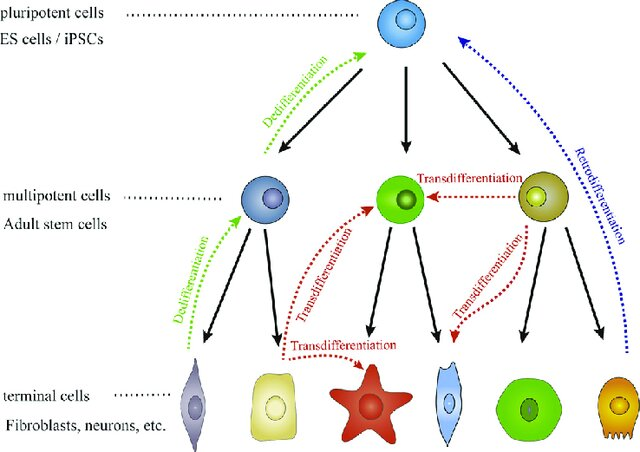
\includegraphics[width=0.65\textwidth]{Figures/transdifferentiation.jpg}
  \caption{\textbf{Cell differentiation.} From~\cite{Wang2012}. The figure illustrates examples of, and differences among, cell differentiation, dedifferentiation, and transdifferentiation.}
  \label{fig:transdifferentiation}
\end{figure}

The organism's need for cell differentiation is communicated via \emph{signalling pathways}~\cite{bradshaw2010}. These signals are transmitted via cascades of biochemical reactions, predominantly through protein phosphorylation catalyzed by protein kinases. Such signalling dynamics can be modelled using Boolean networks. If we can identify the signals that promote dedifferentiation or transdifferentiation, we may be able to emulate them and artificially induce the corresponding cellular transition. This procedure is known as \emph{cell reprogramming}. In this context, finding efficient perturbations for controlling BNs provides an abstract formulation of the signal-identification problem.

\emph{T-cells} are a central component of the human immune system. They must differentiate rapidly to mount an effective immune response. However, diseases affecting the  immune or haematopoietic system (e.g., leukaemia) can disrupt the signalling pathways that regulate T-cell differentiation, making treatment difficult. Cell reprogramming approaches may help identify dysregulated signals and support the development of therapeutic interventions~\cite{Miskov-Zivanovra97, Saadatpour2011, Zanudo2015}.

Another important target for cell reprogramming is \emph{embryonic stem cells}. Because these cells can differentiate into many cell types, they hold considerable clinical promise for applications such as the treatment of diabetes and heart disease, as well as modulation of tumour-related processes and undesired immune responses~\cite{Herberts2011, Singh2009, Takahashi2006, Young2011, Wernig2007}.

There are many additional potential applications of cell reprogramming. Examples include the conversion of white adipocytes to brown-like adipocytes as a potential therapy for obesity~\cite{zhu2015}, restoration of malfunctioning cells~\cite{motter2008}, and, potentially, regeneration or repair of organs~\cite{goligorsky2019}. For these reasons, we consider the \PBN{} control problem to be a timely and broadly applicable research direction.

\section{Myeloid case study}
\label{sec:myeloid_case_study}

\begin{figure}[htb]
\checkoddpage
\edef\side{\ifoddpage l\else r\fi}
\makebox[\textwidth][\side]{% 
	\begin{minipage}{\fullwidth}
    \centering
    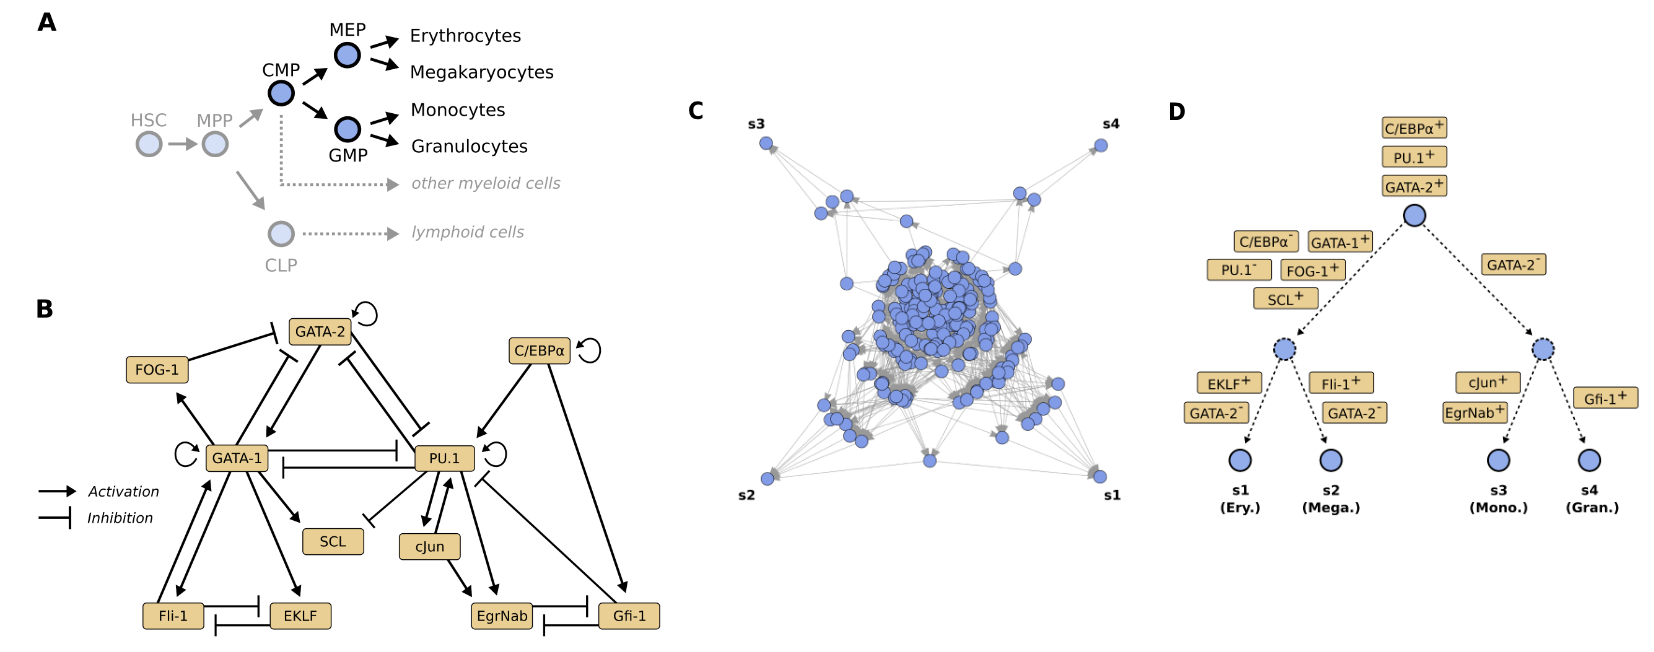
\includegraphics[width=\textwidth]{Figures/myeloid.png}
    \caption{\textbf{Myeloid cell differentiation.} From~\cite{Krumsiek2011}. The figure illustrates what differentiation process is exhibited by the model (A), the regulatory network of the model (B), a visualization of the state space of the model (C), and the deciding update factors driving a cell from common myeloid progenitor (CMP) to the specific phenotypes (D).}
    \label{fig:myeloid}
  	\end{minipage}
	}
\end{figure}

To demonstrate an example of how the control of \PBN{} can be applied to cell reprogramming, we consider a case study of myeloid cell differentiation. Myeloid cells are a type of blood cell that can differentiate into various cell types, including erythrocytes, megakaryocytes, monocytes, and granulocytes. Understanding the regulatory mechanisms underlying myeloid differentiation is crucial for developing therapies for diseases such as leukaemia and other blood disorders. We will be using model from~\cite{Krumsiek2011}. The model has 11 variables and its regulatory network along with the model semantics can be seen in the \autoref{fig:myeloid}. 

\sethlcolor{green!30}
\begin{table}[htbp!]
\small
\centering
\caption{\textbf{Attractor states of myeloid model}. All attractor sizes are 1 and represent four types of specialized blood cells. Values are binary and represent value assignments of model variables. The \hl{highlighted values} represent the differentiating factor for each cell type that is considered in the phenotype specification later.}
\label{tab:myeloid_attractors}
\begin{tabular}{p{1.3cm}w{c}{1.9cm}w{c}{2.3cm}w{c}{1.9cm}w{c}{1.9cm}}
\hline
 & \textbf{Erythrocyte} & \textbf{Megakaryocyte} & \textbf{Monocyte} & \textbf{Granulocyte} \\
\hline
CEBPa   & 0 & 0 & 0 & 1 \\
\cellcolor{green!30}EKLF    & \cellcolor{green!30}1 & 0 & 0 & 0 \\
EgrNab  & 0 & 0 & 1 & 0 \\
FOG1    & 1 & 1 & 0 & 0 \\
\cellcolor{green!30}Fli1    & 0 & \cellcolor{green!30}1 & 0 & 0 \\
GATA1   & 1 & 1 & 0 & 0 \\
GATA2   & 0 & 0 & 0 & 0 \\  
\cellcolor{green!30}Gfi1    & 0 & 0 & 0 & \cellcolor{green!30}1 \\
PU1     & 0 & 0 & 1 & 1 \\
SCL     & 1 & 1 & 0 & 0 \\
\cellcolor{green!30}cJun    & 0 & 0 & \cellcolor{green!30}1 & 0 \\
\hline
\label{tab:myeloid_attractors}
\end{tabular}
\end{table}

We use AEON.py~\cite{aeonpy} to do the analysis of the model and to compute the control. First, we do a standard attractor search to find the attractors of the model. The binary single-state attractors are shown in~\autoref{tab:myeloid_attractors}. Even though the tool does not tell us the semantics of the attractors, we can identify them by comparing the attractor states with the known phenotypes of the myeloid differentiation. The single differentiating factor for each cell type is highlighted in the table.

Since we have results from the attractor search, we can perform the source-target control for all the attractor pairs. The presumption is that eventually the cell converges to one of the possible attractors and that using source-target control we can find perturbations which can drive the cell from one attractor to another. The results of the control are shown in \autoref{tab:myeloid_st}. We can see that in some cases one-step perturbations are bigger than temporary or permanent perturbations. The worst case is reprogramming from megakaryocytes to granulocytes, where one-size perturbation needs to be of size 4 while temporary or permanent perturbation suffice with size 2. Also, even though temporary and permanent perturbation are of the same size, for some cases there are more options for temporary perturbations than for permanent ones.


\begin{table}[htb]
\centering
\footnotesize
\setlength{\tabcolsep}{4pt}
\checkoddpage
\edef\side{\ifoddpage l\else r\fi}
\makebox[\textwidth][\side]{% 
\begin{minipage}[t]{\fullwidth}
\caption{\textbf{Source-target control between attractors.} Perturbation values are written as $\var{x}\shorteq1$ (True) and $\var{x}\shorteq0$ (False). When a perturbation contains multiple assignments, they are grouped in braces $\{\cdot\}$.}
\resizebox{\textwidth}{!}{
\begin{tabular}{llp{4.6cm}p{4cm}p{4cm}}
\hline
\textbf{Source} & \textbf{Target} & \textbf{One-step} & \textbf{Temporary} & \textbf{Permanent} \\
\hline
Ery. & Mega.
& \{\var{EKLF}${\shorteq}0$,\var{Fli1}${\shorteq}1$\}
& \var{Fli1}${\shorteq}1$;\var{EKLF}${\shorteq}0$
& \var{Fli1}${\shorteq}1$;\var{EKLF}${\shorteq}0$ \\

Ery. & Mono.
& \var{PU1}${\shorteq}1$
& \var{PU1}${\shorteq}1$
& \var{PU1}${\shorteq}1$ \\

Ery. & Gran.
& \{\var{CEBPa}${\shorteq}1$,\var{GATA1}${\shorteq}0$,\var{Gfi1}${\shorteq}1$\}
& \{\var{CEBPa}${\shorteq}1$,\var{cJun}${\shorteq}0$\};\
& \{\var{CEBPa}${\shorteq}1$,\var{cJun}${\shorteq}0$,\var{Gfi1}${\shorteq}1$\}\\
& & & \{\var{CEBPa}${\shorteq}1$,\var{EgrNab}${\shorteq}0$\}; & \{\var{CEBPa}${\shorteq}1$,\var{EgrNab}${\shorteq}0$\}; \\
& & & \{\var{CEBPa}${\shorteq}1$,\var{Gfi1}${\shorteq}1$\} & \{\var{CEBPa}${\shorteq}1$,\var{Gfi1}${\shorteq}1$\}\\

Mega. & Ery.
& \{\var{EKLF}${\shorteq}1$,\var{Fli1}${\shorteq}0$\}
& \var{Fli1}${\shorteq}0$;\ \var{EKLF}${\shorteq}1$
& \var{Fli1}${\shorteq}0$;\ \var{EKLF}${\shorteq}1$ \\

Mega. & Mono.
& \var{PU1}${\shorteq}1$
& \var{PU1}${\shorteq}1$
& \var{PU1}${\shorteq}1$ \\

Mega. & Gran.
& \{\var{CEBPa}${\shorteq}1$,\var{Gfi1}${\shorteq}1$,\var{PU1}${\shorteq}1$,\var{SCL}${\shorteq}0$\}
& \{\var{CEBPa}${\shorteq}1$,\var{cJun}${\shorteq}0$\};\ 
& \{\var{CEBPa}${\shorteq}1$,\ \var{cJun}${\shorteq}0$\};\ \\

&  & \{\var{CEBPa}${\shorteq}1$,\var{Gfi1}${\shorteq}1$,\var{PU1}${\shorteq}1$,\var{GATA1}${\shorteq}0$\} & \{\var{CEBPa}${\shorteq}1$,\var{EgrNab}${\shorteq}0$\}; & \{\var{CEBPa}${\shorteq}1$,\var{EgrNab}${\shorteq}0$\};  \\
&  & \{\var{CEBPa}${\shorteq}1$,\var{Gfi1}${\shorteq}1$,\var{Fli1}${\shorteq}0$,\var{GATA1}${\shorteq}0$\} & \{\var{CEBPa}${\shorteq}1$,\var{Gfi1}${\shorteq}1$\} & \{\var{CEBPa}${\shorteq}1$,\var{Gfi1}${\shorteq}1$\} \\

Mono. & Ery.
& \{\var{EKLF}${\shorteq}1$,\var{GATA1}${\shorteq}1$,\var{PU1}${\shorteq}0$\}
& \{\var{Fli1}${\shorteq}0$,\ \var{GATA2}${\shorteq}1$,\ \var{PU1}${\shorteq}0\};\ \dots$
& \{\var{Fli1}${\shorteq}0$,\ \var{GATA2}${\shorteq}1$,\ \var{PU1}${\shorteq}0\};\ \dots$ \\
& & & $\dots$ \textit{5 more options} & \{\var{EKLF}${\shorteq}1$,\ \var{GATA2}${\shorteq}1$,\ \var{PU1}${\shorteq}0$\};\ \\

Mono. & Mega.
& \{\var{Fli1}${\shorteq}1$,\var{GATA1}${\shorteq}1$,\var{PU1}${\shorteq}0$\}
& \{\var{PU1}${\shorteq}0$,\ \var{Fli1}${\shorteq}1$\}
& \{\var{Fli1}${\shorteq}1$,\ \var{PU1}${\shorteq}0$\} \\

Mono. & Gran.
& \{\var{CEBPa}${\shorteq}1$,\var{EgrNab}${\shorteq}0$,\var{Gfi1}${\shorteq}1$\}
& \{\var{CEBPa}${\shorteq}1$,\ \var{cJun}${\shorteq}0$\};
& \{\var{CEBPa}${\shorteq}1$,\ \var{cJun}${\shorteq}0$\}; \\
& & & $\dots$ \textit{3 more options} & $\dots$ \textit{2 more options} \\

Gran. & Ery.
& \{\var{CEBPa}${\shorteq}0$,\var{EKLF}${\shorteq}1$,\var{GATA1}${\shorteq}1$,\var{PU1}${\shorteq}0$\} 
& \{\var{Fli1}${\shorteq}0$,\var{GATA2}${\shorteq}1$,\var{PU1}${\shorteq}0$\};\ $\dots$
& \{\var{Fli1}${\shorteq}0$,\var{GATA2}${\shorteq}1$,\var{PU1}${\shorteq}0$\};\  \\
& & & $\dots$ \textit{5 more options} & \{\var{EKLF}${\shorteq}1$,\var{GATA2}${\shorteq}1$,\var{PU1}${\shorteq}0$\} \\

Gran. & Mega.
& \{\var{CEBPa}${\shorteq}0$,\var{GATA1}${\shorteq}1$,\var{Fli1}${\shorteq}1$,\var{PU1}${\shorteq}0$\} 
& \{\var{PU1}${\shorteq}0$,\ \var{Fli1}${\shorteq}1$\} 
& \{\var{Fli1}${\shorteq}1$,\ \var{PU1}${\shorteq}0$\} \\

Gran. & Mono.
& \var{CEBPa}${\shorteq}0$ 
& \var{CEBPa}${\shorteq}0$ 
& \var{CEBPa}${\shorteq}0$ \\
\hline
\end{tabular}}
\label{tab:myeloid_st}
\end{minipage}}
\end{table}


\begin{figure}
  \centering
  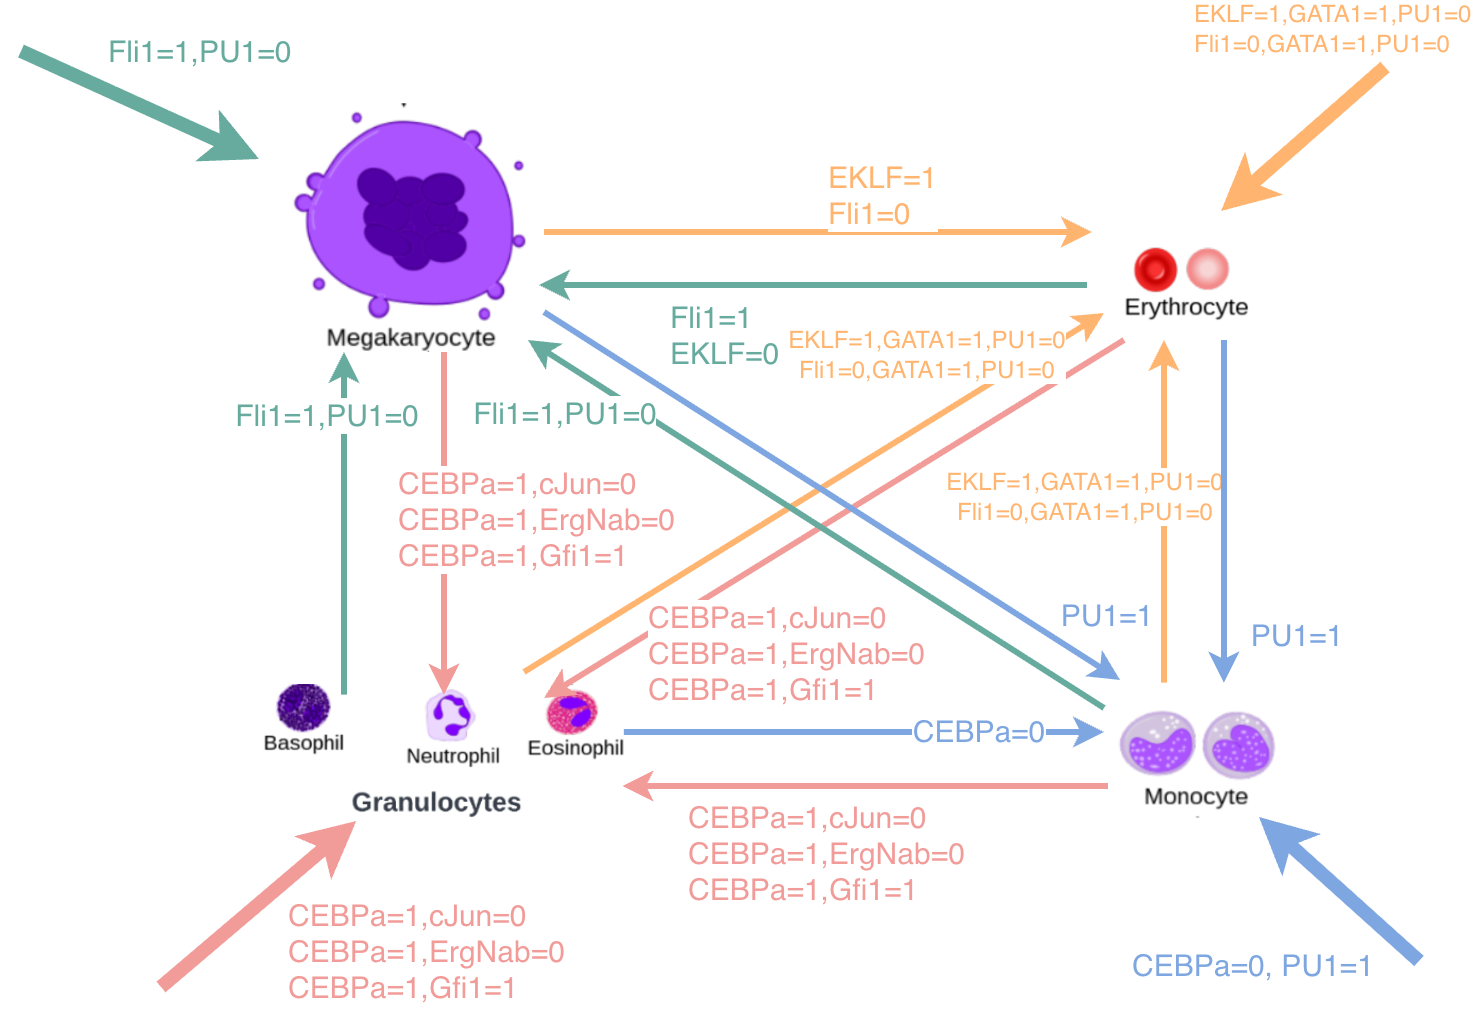
\includegraphics[width=0.9\textwidth]{Figures/myeloid_phenotype.png}
  \caption{\textbf{Control results for myeloid model.} The figure shows the results of control for each cell type in the myeloid model. The arrows going from one cell type to another represent results of permanent source-target control while the arrows going into a cell type (without any source) show results of phenotype control. Each row of the arrow label represents one perturbation. The color of each arrow depends on the control's target -- green for megakaryocytes, blue for monocytes, orange for erythrocytes and red for granulocytes.}
  \label{fig:myeloid_full_control}
\end{figure}

Next, we can also run phenotype control to find the perturbations that stabilize the network regardless of the source attractor. The results of the phenotype control are shown in \autoref{fig:myeloid_full_control}. We can see, that in some cases, like in case of megakaryocytes, the minimal perturbation size is the same for source-target and phenotype control, while with control to other cell types we can fine-tune the perturbation to the known source and use a subset of the complete phenotype perturbation. Nonetheless, the phenotype control is always a superset of the source-target control, which is consistent with the fact that the phenotype control is a more general problem.

Finally, we can briefly compare our results with the source paper of the model that is depicted in \autoref{fig:myeloid}. We can see, that our framework yielded results consistent with the original study, since no perturbation negates the perturbation evolution depicted in branches (the root is only initial state and it can be negated). Sometimes, the negation of factors that are driving to one cell type work as a driver to another cell type, which is consistent with the known biology of the system. For example, the perturbations to erythrocytes can be enabled either by over-expression of EKLF (as depicted in the original study) or by the knock-out of Fli1 which over-expression is driving to megakaryocytes.

\begin{table}[htbp!]
\small
\caption{\textbf{Functions of partially specified myeloid model.} The functions of the original model are shown in the second column, while the functions of the partially specified model are shown in the third column. The symbol `---' means, that the function is not changed. The new functions are defined as functions of the original variables and thus they are consistent with the original model.}
\centering
\begin{tabular}{lll}
\hline
\textbf{Variable} & \textbf{Function} & \textbf{New function}\\
\hline
\var{GATA2} & $\var{GATA2} \land \neg(\var{GATA1} \land \var{FOG1}) \land \neg{\var{PU1}}$ & $f(\var{GATA2}, \var{GATA1}, \var{FOG1}, \var{PU1})$ \\
\var{GATA1} & $(\var{GATA1} \lor \var{GATA2} \lor \var{Fli1}) \land \neg{\var{PU1}}$ &  --- \\
\var{FOG1} & $\var{GATA1}$ & --- \\
\var{EKLF} & $\var{GATA1} \land \neg\var{Fli1}$ & --- \\
\var{Fli1} & $\var{GATA1} \land \neg\var{EKLF}$ & --- \\
\var{SCL} & $\var{GATA1} \land \neg\var{PU1}$ & --- \\
\var{CEBPa} & $\var{CEBPa} \land \neg(\var{GATA1} \land \var{FOG1} \land \var{SCL})$ & $g(\var{CEBPa}, \var{GATA1}, \var{FOG1}, \var{SCL})$ \\
\var{PU1} & ($\var{CEBPa} \lor \var{PU1}) \land \neg(\var{GATA1} \lor \var{GATA2})$ & $h(\var{CEBPa}, \var{PU1}, \var{GATA1}, \var{GATA2})$ \\
\var{cJun} & $\var{PU1} \land \neg\var{Gfi1}$ & --- \\
\var{EgrNab} & $(\var{PU1} \land \neg\var{cJun}) \land \neg\var{Gfi1}$ & --- \\
\var{Gfi1} & $\var{CEBPa} \land \neg\var{EgrNab}$ & --- \\
\hline
\label{tab:myeloid_funs}
\end{tabular}
\end{table}

In order to fully demonstrate the capability of the developed methods, we decided to simulate partial specification of the model by arbitrarily introducing some unknown functions in the model. The model adjustments can be seen in \autoref{tab:myeloid_funs}.


\begin{figure}[htbp!]
  \centering
  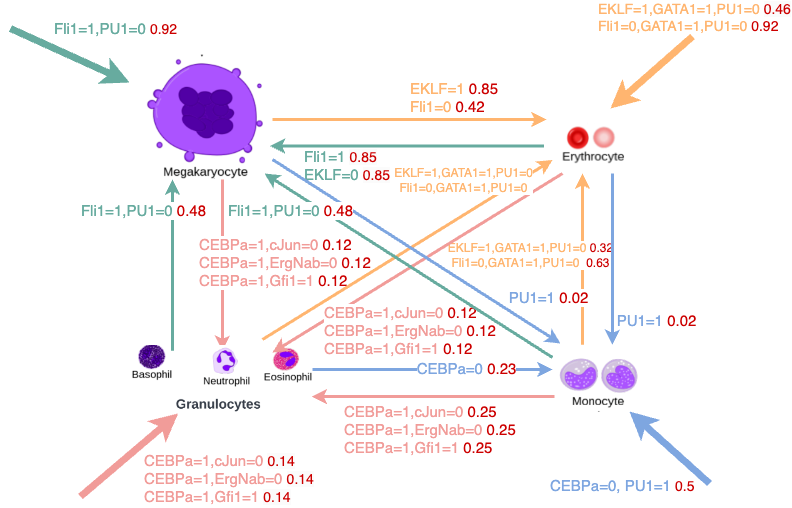
\includegraphics[width=\textwidth]{Figures/myeloid_perturbations_robustness.png}
  \caption{\textbf{Control results for partially specified myeloid model.} The figure shows the results from \autoref{fig:myeloid_full_control} in the partially specified model. The considered perturbations are the equal to the ones in the fully specified model, but they are also labelled with the robustness in the partially specified model.}
  \label{fig:myeloid_full_control_adjusted}
\end{figure}

However, attractor analysis of the partially specified model revealed that some attractors satisfy multiple phenotype specifications when phenotypes are defined by the expression of a single marker. For example, there was an attractor that had \var{EKLF}$\shorteq1$ and $\var{Gfi1}\shorteq1$, therefore it was shared between erythrocytes and granulocytes. To resolve this issue, we adjust the phenotype specification to require only one marker to be set to true, while other markers were required to be false. For example, the phenotype specification for erythrocytes was changed from $\var{EKLF}\shorteq1$ to $\var{EKLF}\shorteq1 \land \var{Fli1}\shorteq0 \land \var{Gfi1}\shorteq0 \land \var{cJun}\shorteq0$. This adjustment ensured that the phenotypes are disjoint, and thus we can perform the control analysis without any issues. The results of the control in the partially specified model are shown in \autoref{fig:myeloid_full_control_adjusted}. 

What is interesting, is that phenotype control in some cases, despite being global and therefore solving a harder problem in a sense has more robust perturbation than source-target control (for example, for megakaryocytes or monocytes). This is because the source-target control is more restrictive and requires stabilization in one specific state, while the phenotype control requires stabilization allows for stabilization in any state of the phenotype, which is more flexible and robust toward model uncertainty. This well illustrates the advantage of the phenotype control over the source-target control in the context of model uncertainty. 

In this section we have seen, that introducing uncertainty into the model can lead to unexpected behaviors of the model, such as shared attractors between phenotypes. This can be seen as an example of how the model uncertainty can lead to a loss of model precision. In the next section, we will show how the control can be used to guide the model refinement and thus to lower the model uncertainty and increase the model precision.


\section{Control workflow for therapy and model refinement}
\label{sec:control_workflow}

\begin{figure}[htbp!]
\checkoddpage
\edef\side{\ifoddpage l\else r\fi}
\makebox[\textwidth][\side]{% 
	\begin{minipage}{\fullwidth}
    \centering
    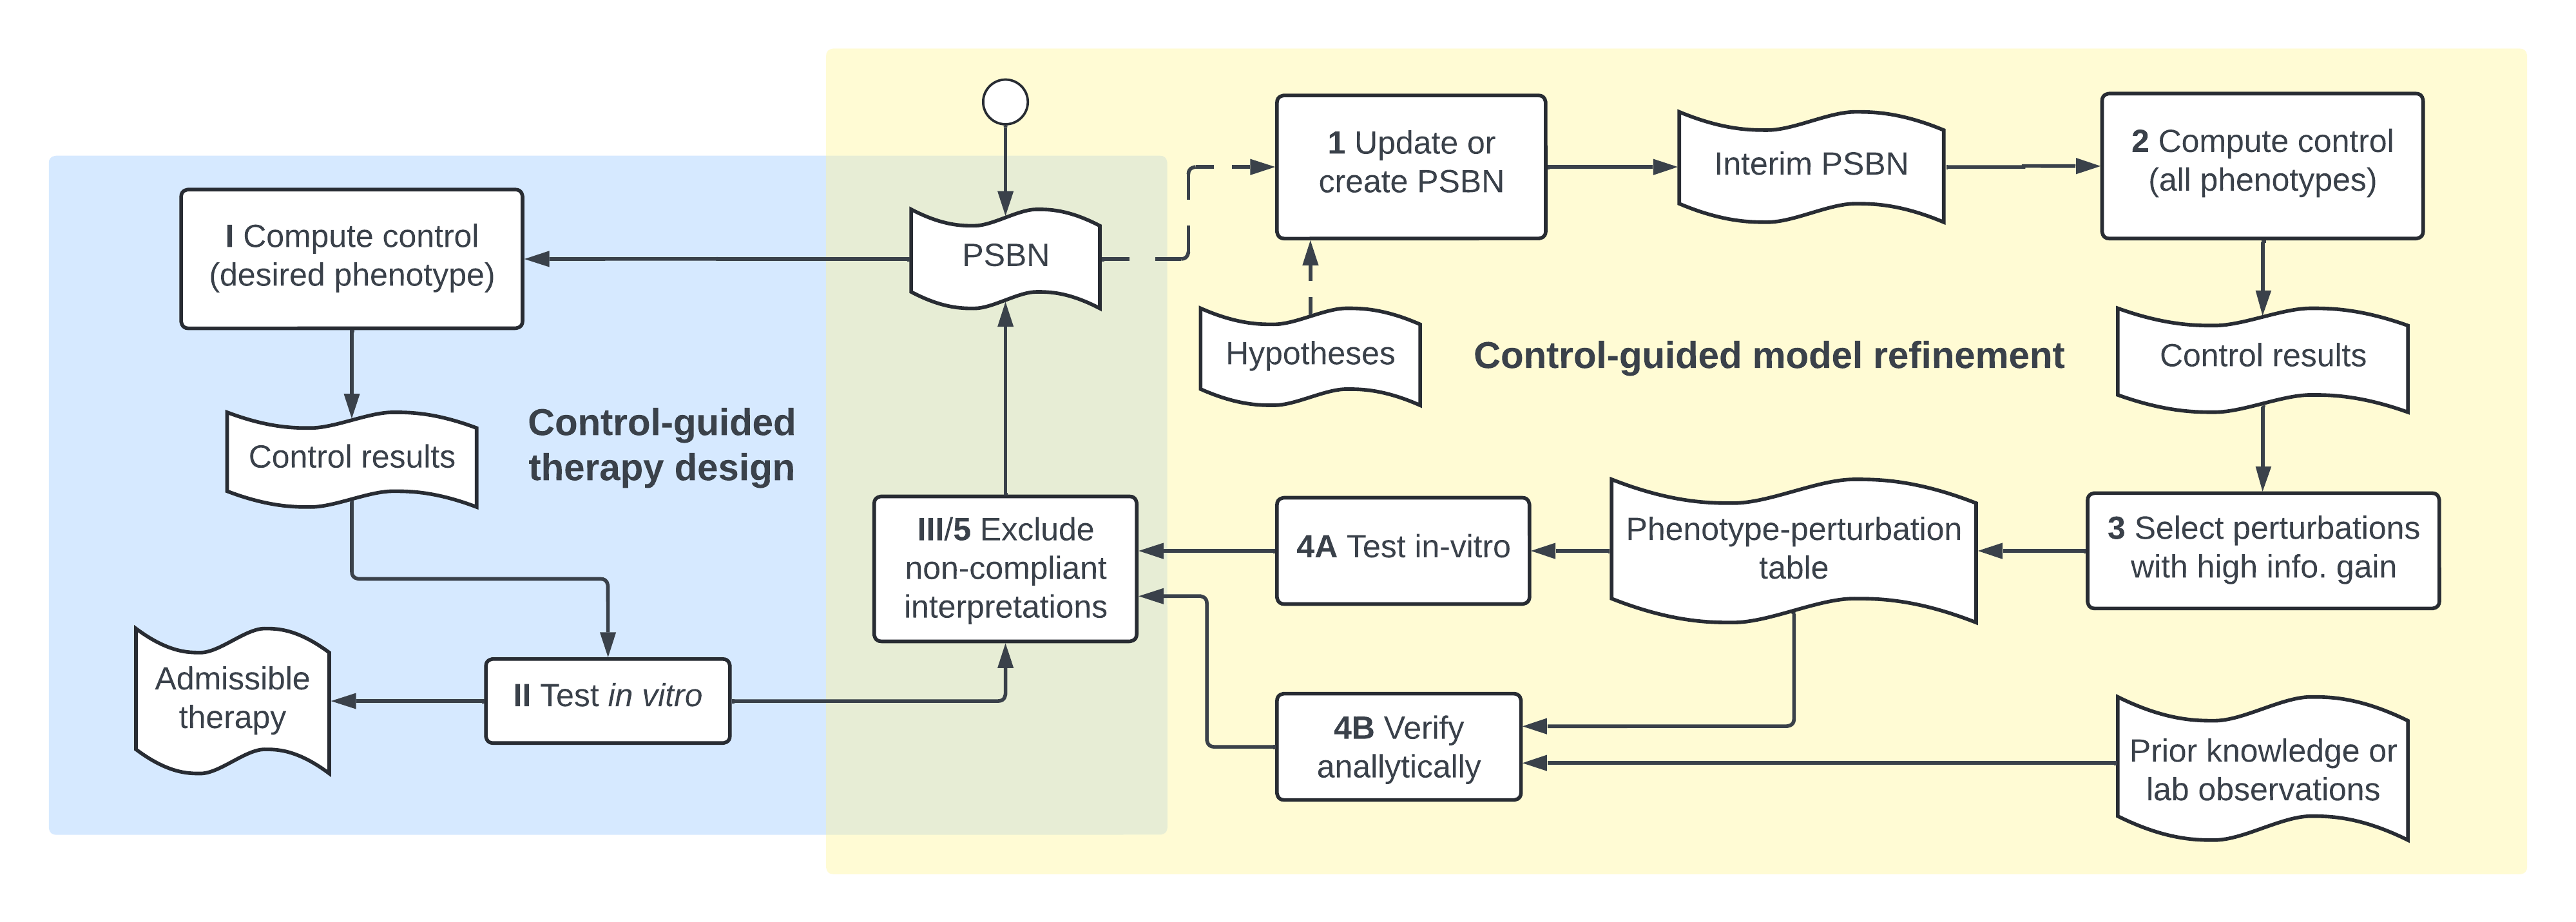
\includegraphics[width=\textwidth]{Figures/control_workflow3.png}
    \caption{\textbf{Workflows of control framework.} The diagram in the picture depicts two workflows of how the phenotype control can be used to achieve two different goals -- to find a therapy or to refine a PSBN model. The workflows can be combined or achieve each other's goals as a side effect (e.g., we might refine model after refuting that the obtained therapy works). The rectangle boxes represent the steps of the workflow, while the tape shaped boxes represent the artifacts obtained from the conducted steps.}
    \label{fig:control_workflow}
  	\end{minipage}
	}
\end{figure}

In this section, we will zoom in on the practical workflow of how the control of partially specified Boolean networks can be used to design a therapy or to refine the model. The workflow is depicted in \autoref{fig:control_workflow}. We will explain the two main branches of the workflow -- control-driven therapy design and control-guided model refinement. We will also show how these two branches can be combined and how they can benefit each other.

\subsection{Control-driven therapy design}

In the previous sections, we have demonstrated the application of \PBN{}  control in context of cell reprogramming. In general, we can refer to this process as \emph{therapy design} in case the goal is to find a suitable treatment which achieves a desired (healthy) system behavior~\cite{Bloomingdale2018, Kim2017, Mendez2017,Saadatpour2011, Zhu2016}. 

Also, as we have seen that such an objective can be directly translated to the phenotype control problem where the system behavior is described via PSBN and the target behavior via a phenotype. The output of the control problem is a set of perturbations which can be implemented back to the real-world, for example as gene knockouts and over-expressions. 


In an ideal case, the artifact obtained from this workflow is a therapy design that can be proven to work in in-vitro (or in-vivo) experiments. Usually, the preferred perturbations are the ones which are easiest to implement in practice (i.e., with the smallest perturbations or the ones which are the most biologically feasible)~\cite{Su2019CMSB}. The second criterion to consider is an expected chance of the therapy to work. This aspect is estimated by the model via a robustness metric of the perturbation~\cite{brim2022}. 

Nonetheless, since the model is imprecise to some extent, the designed therapy might not work in practice. In such case the observations from the experiment can be used to refine \PBN{} model. Usually, we can simply refute the interpretations which do not comply with obtained observation. For example, if we expected a perturbation \var{FGFR3}=1 to stabilize the network in a phenotype \var{ERK}=1 for 60\% of interpretations, but the real-world experiment do not stabilize this phenotype under \var{FGFR3} over-expression, we can conclude, that these 60\% of interpretations are not representing the studied system correctly, and thus we can discard them from the considered set of interpretations. This would complete the workflow cycle depicted on the left side of the diagram in \autoref{fig:control_workflow} and we can attempt to recompute the therapy design with the remaining interpretations.

\subsection{Control-guided model refinement}

In more complex cases, it is also possible, that the treatment is not replicated in vitro even for a perturbation with 100\% robustness. As a result, we might need to rework the model significantly, e.g., by introducing new model parts (regulations and variables) or by changing the existing components. Typically, these model adjustments significantly expand unknown parts of the model, since they are based on hypotheses and uncertainty. Then, a typical next step is verification of the hypotheses we posed as well as efforts to lower the introduced uncertainty. 

As shown on the right side of the diagram in \autoref{fig:control_workflow}, we use phenotype control to guide an experimental design of knockout or over-expression experiments for the model refinement~\cite{UdDean2016}. Let us zoom in to the details of this process.

\paragraph{Initial \PBN{} model}
We start with an initial \PBN{} model (Step 1; Fig. \autoref{fig:control_workflow}) and its phenotypes. Such \PBN{} can be constructed directly from prior knowledge and known assumptions about biological behavior, or it can be an extension of some existing model relying on new information (e.g., newly discovered regulations or pathways).

\paragraph{Screening admissible perturbations}
We analyze the feasible perturbations w.r.t. known phenotypes of the \PBN{} (Step 2; \autoref{fig:control_workflow}). In therapy design, we would seek perturbations of high robustness achieving our phenotype of interest. For refinement, perfect robustness (i.e., $\rho(Q) = 1.0$) is \emph{not} desirable as it means the perturbed interpretations are indistinguishable through phenotype observations. Similarly, if two perturbations achieve equivalent phenotypes across all interpretations, only one needs to be considered further.

\paragraph{Selection of perturbations using information-gain}

While the initial screening can significantly reduce the space of admissible perturbations, it likely still remains too large to explore \emph{in vitro}. We therefore prioritize perturbations using a \emph{normalized mutual information score} (NMIS; \cite{Kent83}), quantifying how well is the outcome of a perturbation explained by a specific unknown \emph{feature} of the \PBN{} (Step 3;  \autoref{fig:control_workflow}). We use the following formulas to compute the NMIS:

$$
IS(X; Y) = \sum_{x, y} P(x, y) \log \frac{P(x, y)}{P(x) P(y)}
$$
$$
H(X) = -\sum_{x} P(x) \log P(x)
$$
$$ 
NMIS(X; Y) = \frac{2 IS(X; Y)}{H(X) H(Y)} 
$$

To compute NMIS, we observe that interpretations $\allInterpretations$ can be partitioned into equivalence classes $\interpretationSet_1, \ldots, \interpretationSet_k$ based on their outcomes, with each class consisting of interpretations that are indistinguishable by any admissible perturbation. Each class is assigned a set of \emph{behavior labels} and \emph{feature values}. 

Here, behavior labels correspond to the phenotypes observed when subject to individual perturbations (collectively, we call these the \emph{behavior pattern} of $\interpretationSet_i$). Similarly, \emph{feature values} are based on selected properties of the underlying class of networks~$\interpretationSet_i$. These features are derived from the unknown elements of the \PBN{}, such as the uninterpreted update functions or properties of regulations (essentiality, monotonicity, canalization, etc.).

We use NMIS to express the mutual information between the behavior labels achieved by a perturbation $Q$ and the values given by a particular network feature, quantifying how well the network feature predicts the outcome of perturbation $Q$.

High NMIS for a feature-perturbation pair indicates that observing the perturbed phenotypes should (with high likelihood) either confirm or refute that network feature. The perturbation with the highest NMIS (for some network feature) is selected for \emph{in vitro} testing (Step 4A; Fig.~\ref{fig:control_workflow}). Alternatively, prior knowledge can be introduced to assert the expected phenotypes of the model under perturbation (Step 4B; Fig.~\ref{fig:control_workflow}).

Finally, model instances that do not conform to the expected behavior are excluded (Step 5; Fig.~\ref{fig:control_workflow}), allowing us to restart the workflow with an updated \PBN{}.


% As opposed to the therapy design, in this case, we typically focus on perturbations which are the most informative, i.e., the ones which will help us to distinguish between the interpretations the most. More specifically, a perturbation which works for exactly same interpretations is not very informative, since we expect, that it works for all interpretations and thus would not help us lower the model uncertainty (number of interpretations). 

\paragraph{Example of perturbation selection}

For example, let us suppose, that we consider some \PBN{} $\pbnMath$ \emph{similar} to the one from example in \autoref{fig:psbn} (i.e., a \PBN{} with multiple variables and functional symbols). The \PBN{} has 2820 interpretations. and that we compute stabilization in prolifertion (P) phenotype. The result of the control could be perturbations $\perturbation_A, \perturbation_B, \perturbation_C$, while the union of the interpretations for which they work is exactly $\allInterpretations(\pbnMath)$. The cardinality and intersection of the interpretations they cover are shown in \autoref{subfig:set_example}. 

\begin{figure}[ht!]
  \checkoddpage
  \edef\side{\ifoddpage l\else r\fi}
  \makebox[\textwidth][\side]{% 
	\begin{minipage}[t]{\fullwidth}
  \centering
  \subfloat[Interpretation sets controlled by perturb. $\perturbation_A, \perturbation_B, \perturbation_C$.]{
    \begin{minipage}[t]{0.35\textwidth}
      \label{subfig:set_example}
      \vspace{-50pt}% <-- forces top alignment
      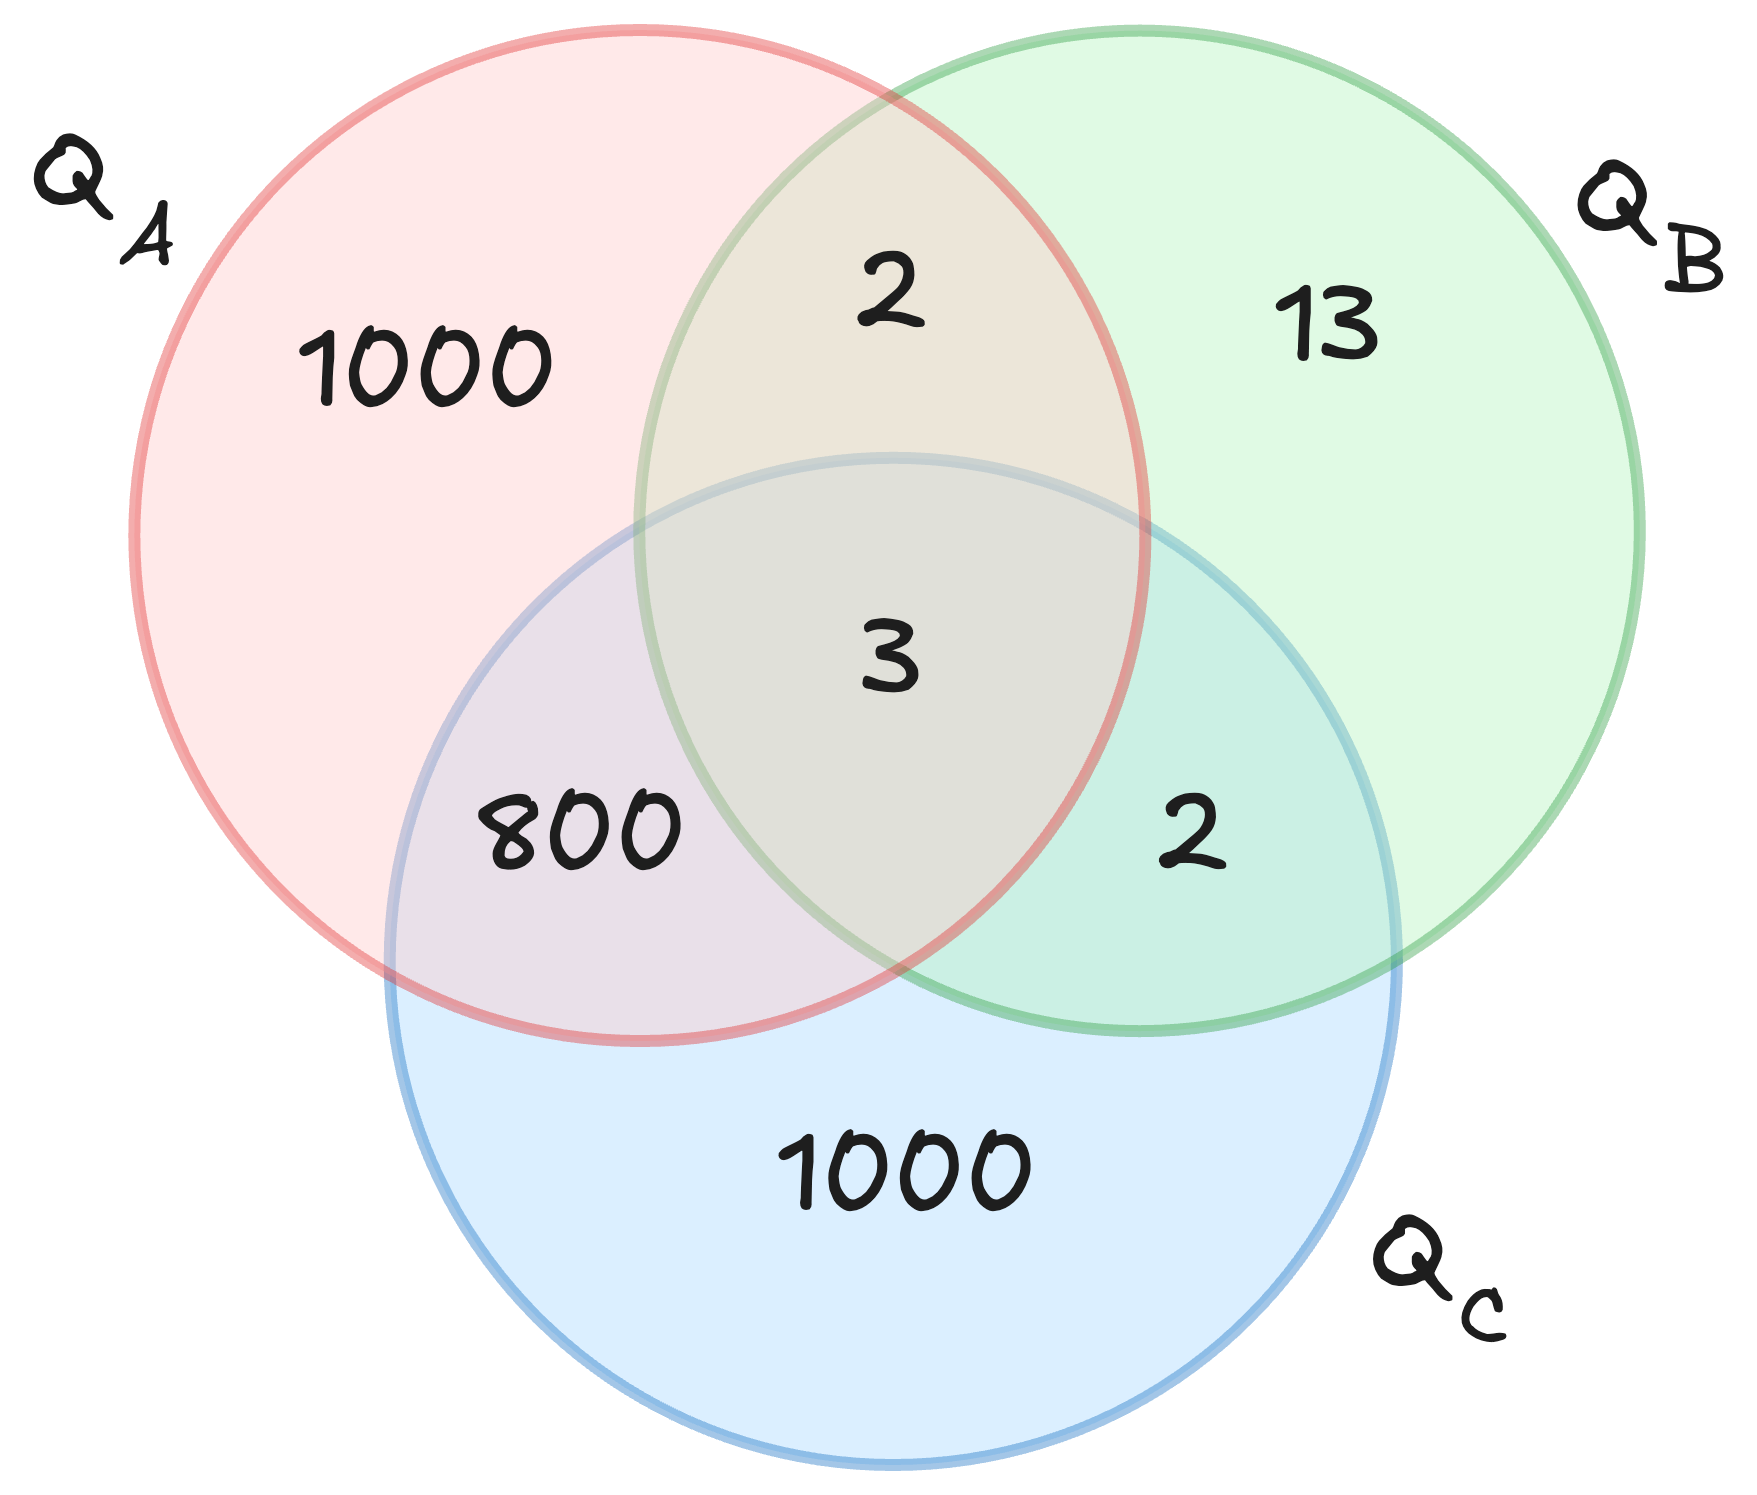
\includegraphics[width=\textwidth]{Figures/perturbations_venn_example.png}
    \end{minipage}
  }~~~~~~~~~~~~~~
  \subfloat[Phenotype-perturb. table for selection of $\perturbation_A$ and $\perturbation_B$.]{
    \begin{minipage}[b]{0.2\textwidth}
      \begin{tabular}{ccl}
      $Q_A$ & $Q_B$ & $\mid \interpretationSet \mid$ \\
      P     & P     & 5               \\
      P     & A  & 1800            \\
      A     & P    & 15              \\
      GA     & A    & 1000           
      \end{tabular}
    \end{minipage}
    \label{subfig:select_a_b}
  }~~~~~~~~~~~~~~
  \subfloat[Phenotype-perturb. table for selection of $\perturbation_A$ and $\perturbation_C$.]{
  \begin{minipage}[b]{0.2\textwidth}
    \begin{tabular}{ccl}
      $\perturbation_A$ & $\perturbation_C$ & $\mid \interpretationSet \mid$ \\
      P    & P & 803             \\
      P    & A  & 1002            \\
      A    & P   & 1002            \\
      A    & A  & 13             
      \end{tabular}
    \end{minipage}
    \label{subfig:select_a_c}
  }
  \vspace*{2mm}
  \caption{
    \textbf{An example of interpretations partitioning of working perturbations.} \autoref{sub@subfig:set_example} shows sets of interpretations and their intersections for some three distinct perturbations $\perturbation_A, \perturbation_B, \perturbation_C$. Then, the \autoref{sub@subfig:select_a_b} and \autoref{sub@subfig:select_a_c} show phenotype-perturbation matrices if perturbations $\perturbation_A$ and $\perturbation_B$ are selected or $\perturbation_A$ and $\perturbation_C$ respectively. Each row represents a set of interpretations. The values in the table cells contain a phenotype in which model stabilizes under the given perturbation one of proliferation (P), apoptosis (A) or growth arrest (GA). The last column contains cardinality of the relevant interpretation set.}
  \label{fig:perturbations_example}
  \end{minipage}
  }
\end{figure}

We can notice, that despite the perturbations $\perturbation_A$ and $\perturbation_C$ are working for exactly the same amount of interpretations, they might control very different sets of particular interpretations. If there would be multiple perturbations which work for exactly same interpretations as the perturbation $\perturbation_A$, it is not expected to be informative to use them all in the real-world experiments. Finally, we can see, that the perturbation $\perturbation_B$ is also covering distinct sets of perturbations, although their size is much smaller. 

If we were in the situation, when we would need to select only two perturbations for the real-world experiments (e.g, due to the high experiment price) we can consider the reduced interpretation sets in \emph{perturbation-phenotype tables} depicted in \autoref{subfig:select_a_b} and \autoref{subfig:select_a_c}. The rows of these tables represent non-overlapping interpretation \emph{classes} with distinct \emph{behavior patterns}, while column values show differing phenotype outcomes of these interpretations under the selected perturbations.

When deciding which two perturbations out of three should be kept, we would be probably inclined to select $\perturbation_A$ and $\perturbation_C$ since in the worst (and most probable) case we would reduce the model uncertainty to a third of the original interpretation cardinality. On the other hand, if we would select $\perturbation_A$ and $\perturbation_B$, there would be a chance, that we would reduce the model uncertainty to a very small fraction of the original one, but the expected chances of this are very low. Nonetheless, the in ideal scenario we would be able to try all three perturbations in the real-world experiments, or we would prefer the perturbations which are easier to implement. 

Notice, that in phenotype-perturbation matrix we may not just represent whether the perturbation works or not, but also which phenotype in particular it exhibits. This is particularly useful for the model refinement, since we can then distinguish behavior classes depending on the exhibited phenotype.

Therefore, this table can be then directly used for design of knock-out and over-expression experiments in the real world. Since rows of a table always contain a distinct combination of phenotypes, we expect to be able to match the results from the phenotypes observed in the real-world to one particular row of the phenotype-perturbation table and thus significantly reduce the model uncertainty.

Performing the designed experiments in vitro is an ideal approach to refine the model. However, the experiments are usually costly and might not always be possible to implement. In such cases, we can still observe which model mechanics allow or prevent a perturbation working for some interpretations. For this, purpose, we can infer \emph{features} of an interpretation sets split obtained in the previous step. 

\begin{table}[ht!] 
  \centering
  \begin{tabular}{l|cc|cc}
                  & \multicolumn{2}{c|}{\textbf{Perturbations}} & \multicolumn{2}{c}{\textbf{Features}}                                     \\
  $\mid \interpretationSet \mid$ & $\perturbation_A$ & $\perturbation_C$ & $\exists \interpretation \in \interpretationSet.$ \var{ERK} $\rightarrow$ \var{FRS2} & $\forall \interpretation \in \interpretationSet . \var{FGFR3} = 0$ \\
  \hline
   803  & P & P & 1 & 0 \\
   1002 & P & A & 0 & 1 \\
   1002 & A & P & 0 & 0 \\
   13   & A & A & 0 & 1                         
  \end{tabular}
  \caption{\textbf{Example of phenotype-perturbation tables with extracted features.} The table shows the binarized  phenotype-perturbation table for the perturbations $\perturbation_A$ and $\perturbation_C$ from \autoref{fig:perturbations_example}. The table is extended with features extracted from the interpretation sets.}
  \label{tab:perturbation_matrix}
  \end{table}

For example, consider \autoref{tab:perturbation_matrix}, where we have selected two perturbations from the previous example in \autoref{fig:perturbations_example}. In the table, we assume that we have selected perturbations $\perturbation_A$ and $\perturbation_C$. We might be interested in finding out \emph{why} a particular perturbation works for some interpretations and not for the others. For this purpose, we infer the features of the interpretation sets. The vector of phenotypes for perturbations can thus be considered as a \emph{label}, and we can observe their \emph{mutual information gain} metric to measure impact of a feature on the~\cite{Kent83}. Note, that since question we are interested in is whether a perturbation works or not, thus it is more advantageous to consider binary labels (yes/no) for the labels. 
Given a set of interpretations $\interpretationSet$, the features we consider are following:
\begin{itemize}
  \item A regulation is essential in all interpretations $\forall \interpretation \in \interpretationSet.$ \var{GRB2} $\rightarrow$ \var{FGFR3} is observable in \pbnMath(\interpretation).
  \item A regulation is essential in any interpretation $\exists \interpretation \in \interpretationSet.$ \var{GRB2} $\rightarrow$ \var{FGFR3} is observable in \pbnMath(\interpretation).
  \item A presence of a particular function instance in 
  all of the given interpretations ($\forall \interpretation \in \interpretationSet .$\var{FGFR3} $=$ \var{FGFR3\_stimulus} $\land$ $\neg$\var{GRB2}  in \pbnMath(\interpretation)). This way we learn, that a particular function is necessary for the phenotype control to work.
  \item A presence of a particular function instance in any of the given interpretations ($\exists \interpretation \in \interpretationSet.$ \var{FGFR3} $=$ \var{FGFR3\_stimulus} $\land$ $\neg$\var{GRB2} in \pbnMath(\interpretation)). This way we might find, that a particular function is preventing a perturbation from working.
\end{itemize}

Note, that the features can be combined in various ways as well as there might be other features to consider (e.g. monotonity of regulations, or particular values of the function symbols, etc.). A rule of the thumb is to refine as many potentially relevant features as possible. In our example, we can notice, that perturbation $\perturbation_C$ avoids proliferation exactly if an interpretation has update function $\var{FGFR3}$=0. This could be a surprising observation for the modeler since maybe they did not expect $\var{FGFR3}$ function to be so trivial, nor $\perturbation_C$ to have such effect on proliferation. If such is the case, approximately a third of the interpretations can be refuted using the analytical approach only.

In more complex cases, it becomes complicated to assess which single feature can completely predict the observed phenotypes. To quantify an extent to which the phenotype is dependent on a given feature we use the mutual information gain metric. Therefore, we consider a single vector of features at a time, and a single vector of phenotype labels yielded by a perturbation, in order to select features best describing each perturbation, to analytically evaluate mechanics of a given perturbation. Since there might be different cardinality for possible phenotype outcomes (i.e. models and perturbations might achieve different number of varying phenotypes), we use normalization for the mutual information gain~\cite{Vinh2009}. 

To summarize, the workflow in \autoref{fig:control_workflow} can be used to design a therapy, or guide the model refinement, or both. The cycle can be repeated any amount of times while having both of these goals in mind. The main difference between the two workflows is the selection of perturbations for the real-world experiments. In the therapy design, we are interested in the perturbations which are the most likely to work, while in the model refinement, we are interested in the perturbations which are the most informative.

\section{MAPK case study}
\label{sec:mapk_case_study}
% What is MAPK and why is it important
The Mitogen-Activated Protein Kinase (MAPK) signaling pathway is a critical cellular signaling pathway that transmits signals from the cell surface to the nucleus in response to various extracellular or internal stimuli, such as growth factors, cytokines, or DNA damage. This pathway regulates a wide range of cellular processes, including proliferation and apoptosis. The disruption of these regulations can lead to diseases, in particular various types of cancer.

We employ our methodology to analyze three models. First, a small-scale abstract model projecting the current knowledge of FGFR3-ERK signalling is considered. Several reported unknown facts are represented by means of a \PBN{} and control-guided refinement is applied to precise the model with respect to hypothesis suggested in literature. 

Second, we consider a larger-scale model~\cite{Grieco2013} of general MAPK signalling affecting cell proliferation, apoptosis, and growth arrest. Third, we embed FGFR3-ERK mechanism into the model~\cite{Grieco2013}, thus introducing the unknown details of the signalling logics. We explore the extended model further with the control-guided framework.

% % Technical details (AEON.py and notebooks in the appendix)
% All our experiments were conducted using the AEON.py Python package~\cite{aeonpy}, which also contains the implementation of the algorithms described in the previous section. The full source code containing all JuPyter notebooks used for the experiments along with the raw results are available at Zenodo doi \url{10.5281/zenodo.16886814}.

\subsection{Isolated FGFR3 pathway model}
\label{sec:mapk_case_study_isolated}

\begin{figure}[!htbp]
\checkoddpage
\edef\side{\ifoddpage l\else r\fi}
\makebox[\textwidth][\side]{% 
	\begin{minipage}{\fullwidth}
    \centering
  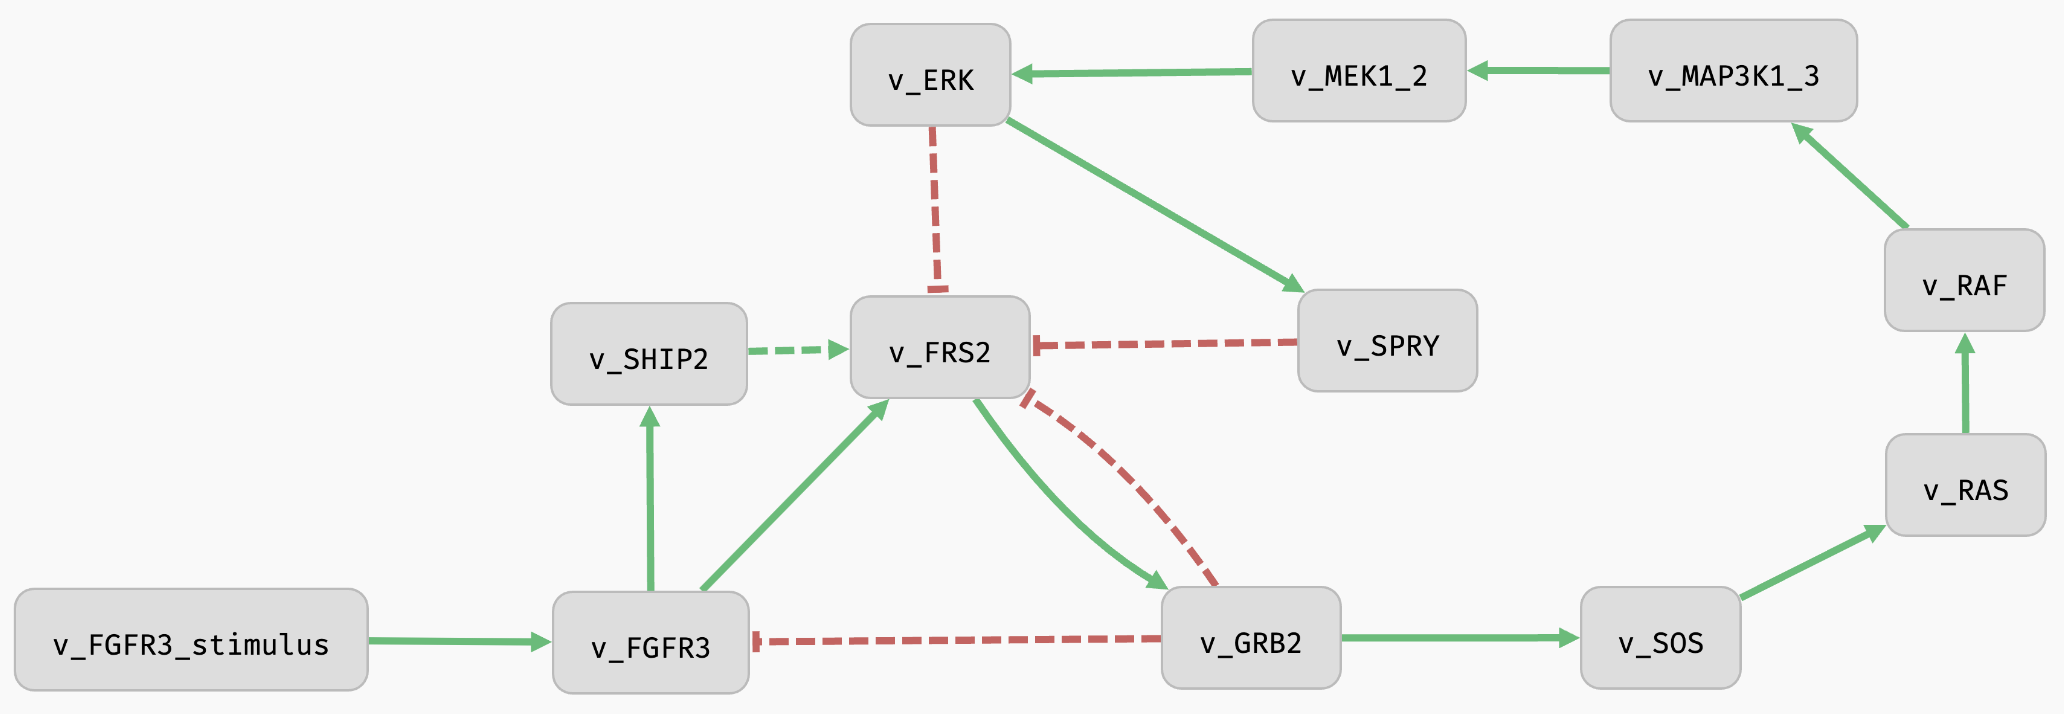
\includegraphics[width=\textwidth]{Figures/fgfr3_isolated.png}
  \caption{\textbf{An isolated FGFR3 pathway model.} The model consists of 12 variables and 16 regulatory interactions. The variables \var{FRS2} and \var{FGFR3}, are partially specified. The positive regulations are depicted in green color while negative regulations are red. The lines which are dashed represent regulations which are not required to be essential in the model interpretations. The model serves as an example for demonstrating the capabilities of our method.}
  \label{fig:fgfr3_isolated}
  \end{minipage}
  }
\end{figure}

Based on our previous research\cite{HSB}, we consider a minimalistic model representing an abstracted form of FGFR3-MAPK signaling pathway, focusing on the interactions among FGFR3, FRS2, SHIP2 and ERK proteins~\cite{Barnat2017}. The model is encoded as a PSBN consisting of 12 variables and 16 regulatory interactions. The model contains one input -- \var{FGFR3\_stimulus}, which is considered implicitly set to true to simulate constitutive activation of the pathway via suitable FGF ligands. This stimulus can be however disabled (perturbed to the value 0) with the phenotype control. The update logics of \var{FGFR3} and \var{FRS2} is partially specified reflecting the fact that the combined effect of variables regulating their activity as well as the presence of particular regulations is not well understood~\cite{Krejci2012,Santhana2023}. 

The dynamics of the final protein component ERK closing the isolated pathway forms the (model) phenotype. In particular, we consider three protein-level phenotypes targeting ERK activity: \var{ERK} stabilization, \var{ERK} avoidance, and \var{ERK} oscillation. Due to the introduced uncertainty, the FGFR3 model has 888 possible interpretations. 

%Using the following observations found in literature we perform control-guided model refinement (as depicted in \autoref{fig:control_workflow}) to exclude biologically inconsistent interpretations of the \PBN{}. Our hypotheses are based on the experimental evidence established with \emph{chondrocyte} cells. 

% \begin{enumerate}
%   \item Oscillation of ERK activity can be observed in some settings \cite{Raina2022}.
%   \item FGF stimulus must be present for ERK activation -- the presence of FGF ligands bond to FGFR3 is \emph{de facto} necessary for FGFR3 activation which in case of the isolated mechanism implies the activation of ERK \cite{Krejci2012}.
%   \item SHIP2 knock-out causes ERK activity to be down-regulated but not suppressed completely \cite{Fafilek2018}.
% \end{enumerate}

% We use these observations as accepted prior knowledge to reduce the number of admissible interpretations of the \PBN{}.

\begin{table}[]
\caption{\textbf{FGFR3 pathway model update functions.} The table shows the update functions of the FGFR3 pathway model. The variables \var{FGFR3} and \var{FRS2} are partially specified, while the rest of the variables are fully specified. The function symbols $f$, $g$ and $h$ are unary function symbols, while $\land$ and $\lor$ are binary logical operators.}
\centering
\begin{tabular}{ll}
\hline
\textbf{Variable}   & \textbf{Function}                                         \\
\hline
\var{FGFR3}      & $f(\var{FGFR3\_stimulus}, \var{GRB2})$                          \\
\var{GRB2}       & \var{FRS2}                                             \\
\var{FRS2}       & $\var{FGFR3} \land g(\var{ERK}, \var{GRB2}, \var{SPRY}) \lor (\var{FGFR3} \land h(\var{SHIP2}))$ \\
\var{ERK}        & \var{MEK1\_2}                                           \\
\var{SHIP2}      & \var{FGFR3}                                            \\
\var{SPRY}       & \var{ERK}                                              \\
\var{SOS}        & \var{GRB2}                                             \\
\var{RAS}        & \var{SOS}                                              \\
\var{RAF}        & \var{RAS}                                              \\
\var{MAP3K1\_3}  & \var{RAF}                                              \\
\var{MEK1\_2}    & \var{MAP3K1\_3}  \\
\hline
\end{tabular}
\label{tab:small_mapk_funs}
\end{table}

\begin{table}[ht!]
  \small
  \caption{\textbf{Phenotype control of the isolated FGFR3 pathway model.} The table shows the perturbations that control the model towards the ERK stabilization, avoidance and oscillation phenotypes. The symbol $\emptyset$ denotes an absence of perturbations. The robustness of each perturbation is of all interpretation of the original model is shown in the third column.}
  \centering
  \resizebox{\textwidth}{!}{
  \begin{tabular}{lll}
    \hline
    \textbf{Phenotype}                 & \textbf{Perturbation}                                                                                            & $\robustness$  \\ \hline
    \multirow{6}{*}{ERK stabilization} & \begin{tabular}[c]{@{}l@{}}\var{FRS2}=1, \var{GRB2}=1, \var{MAPK3K1\_3}=1, \var{MEK1\_2}=1, \\ \var{RAF}=1, \var{RAS}=1, \var{SOS}=1\end{tabular}          & 1                 \\[2.1ex]
                                      & \var{FGFR3}=1                                                                                                          & 0.94                \\[1ex]

                                       & \var{SPRY}=0                                                                                                          & 0.637                \\[1ex]
                                       & \O, \var{SHIP2}=1, \var{SPRY}=1                                                                                                     & 0.626           \\
                                       & \var{SHIP2}=0                                                                                    & 0.583             \\ \midrule
    \multirow{4}{*}{ERK avoidance}     & \begin{tabular}[c]{@{}l@{}}\var{FGFR3}=0, \var{FRS2}=0, \var{GRB2}=0, \var{MAPK3K1\_3}=0,\\ \var{MEK1\_2}=1, \var{RAF}=0, \var{RAS}=0, \var{SOS}=0\end{tabular} & 1             \\[2ex]
                                       & \var{FGFR3\_st.}=0                                                                                                & 0.667     \\[1ex]
                                       & \var{SPRY}=1                                                                                                           & 0.017                 \\ \midrule
    \multirow{8}{*}{ERK oscillation}   & \var{SHIP2}=0                                                                                                          & 0.41                \\[1ex]
                                       & \O, \var{SHIP2}=1                                                             & 0.374           \\[1ex]
                                       & \var{SPRY}=0                                                             & 0.363        \\[1ex]
                                       & \var{SPRY}=1                                                            & 0.357          \\[1ex] 
                                       & \var{FGFR3}=1                                                            & 0.061        \\[1ex] 
                                       & \var{FGFR3\_stimulus}=0                                                            & 0.333     \\[1ex] \midrule

    \end{tabular}}
  \label{tab:fgfr3_isolated}
  \end{table}



Let us we observe the non-perturbed behavior -- the ``natural'' phenotypes of the model. After running a simple algorithm for searching the attractors supported in AEON.py, we learn that the unperturbed model stabilizes in 2 types of attractors -- \var{ERK} stabilization (556 interpretations) and \var{ERK} oscillation (332 interpretations). The \var{ERK} avoidance phenotype was not observed in the non-perturbed version of the model. This is due to the presence of the \var{FGFR3\_stimulus} which we have set to true for our experiments. The stimulus transitively activates \var{ERK} via \var{FGFR3}, \var{FRS2} and other transitive variables.

\paragraph{Initial perturbation screening}

Next, we computed the phenotype control for all three considered phenotypes. The results are summarized in Table~\ref{tab:fgfr3_isolated}. Due to the small size of the model, we list only perturbations up to size one, since perturbations of bigger size did not achieve better results; not even in case of oscillation, where no perturbation has 100\% robustness. Even when perturbations of all sizes were computed, no perturbation achieved better robustness towards oscillation phenotype than \var{SHIP2}=0. This might be due to the incomplete model design, which we will discuss later.

\begin{figure}[ht!]
\captionsetup[subfigure]{justification=centering}
\checkoddpage
\edef\side{\ifoddpage l\else r\fi}
\makebox[\textwidth][\side]{% 
	\begin{minipage}{\fullwidth}
  \centering
  \subfloat[ERK stabilization.]{
    \label{subfig:true_upset}
    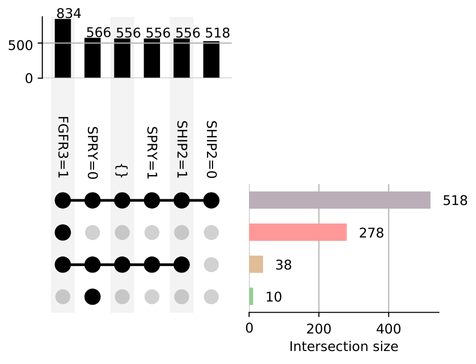
\includegraphics[width=0.5\textwidth]{Figures/fgfr3_isolated_exp/erk_true_upset_colors.png}
  }\hfill
  \subfloat[ERK stabilization - Venn diagram.]{
    \label{subfig:true_venn}
    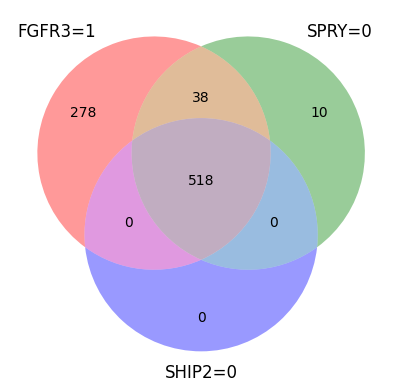
\includegraphics[width=0.4\textwidth]{Figures/fgfr3_isolated_exp/erk_true_venn.png}
  }\hfill
  \subfloat[ERK avoidance.]{
    \label{subfig:false_upset}
    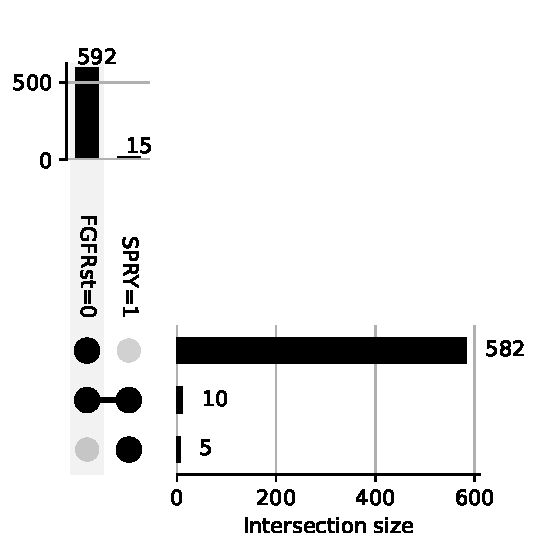
\includegraphics[width=0.35\textwidth]{Figures/fgfr3_isolated_exp/small_fgfr3_isolated_erk_avoidance_upset_full.pdf}
  }
  \subfloat[ERK oscillation.]{
    \label{subfig:oscillation_upset}
    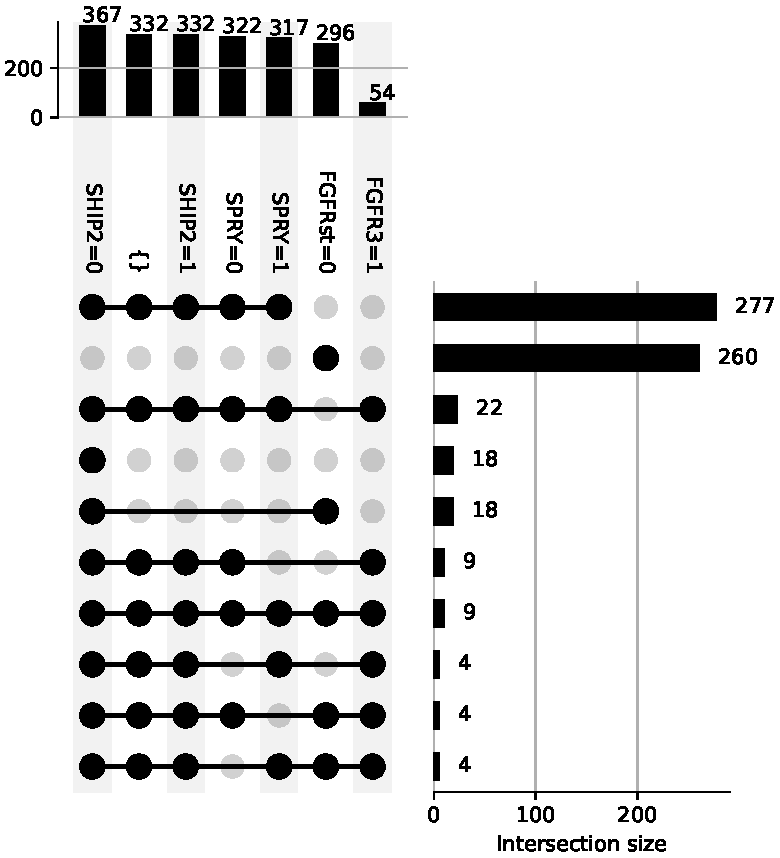
\includegraphics[width=0.6\textwidth]{Figures/fgfr3_isolated_exp/small_fgfr3_isolated_erk_oscillation_compact.pdf}
  }
  \caption{\textbf{Data informing selection of knockout and over-expression experiments to refine model uncertainty.} \autoref{subfig:true_upset},\autoref{subfig:false_upset}, and \autoref{subfig:oscillation_upset} use UpSet plots~\cite{Lex2014} to represent intersections between sets of interpretations controlled by particular perturbations into ERK stabilization, avoidance and oscillation. \autoref{subfig:true_venn} then represent intersections between controlled interpretations by perturbation candidates selected from \autoref{subfig:true_upset}.}
  \label{fig:fgfr3_isolated_exp}
  \end{minipage}
  }
\end{figure}


We can also notice, that perturbation of the same variable to both true and false may lead to the same phenotype (e.g. \var{SPRY} in case of oscillation). Similarly, the same perturbations can lead to multiple phenotypes (e.g. \var{SHIP2}=1). This is because in these cases the partially specified functions have a greater influence on the network dynamics, than the perturbation itself -- thus, another plausible explanation is, that the network behaves the same way as without any perturbations. In case, this is not expected behavior, this can be seen as a flaw introduced in some interpretations of the model which should be therefore refuted.

To probe further all the unexpected model behavior we use the framework of perturbation experiments. First, we need to observe which perturbations yield the most differing results in terms of controlled interpretations. To do this, we can depict intersections of the interpretation sets controlled by various perturbations with a robustness lesser than 100\%. The results of such an analysis are displayed in Fig.~\ref{fig:fgfr3_isolated_exp}. We use Upset plots for the visualization~\cite{Lex2014}.

We can see, that \var{ERK} avoidance case (Subfig.~\ref{subfig:false_upset}) gives us very straightforward answer of which perturbations should be selected, since there are only two perturbations (\var{FGFR3\_stimulus}=0 and \var{SPRY}=1) covering unique sets of interpretations (the same can be seen from Table~\ref{tab:fgfr3_isolated}). 

The case of \var{ERK} stabilization (Subfig.~\ref{subfig:true_upset}) is a bit more complicated, as there are multiple perturbations that could be selected. Nonetheless, we can notice, that \var{SPRY}=0 and \var{FGFR3}=1 should be selected, since they cover some unique set of interpretations. Similarly, \var{SHIP2}=0 should be selected, because it is missing some interpretations covered by all other perturbations (i.e, it is unique by interpretations which it is \emph{not} covering). Finally, as we can see in the Subfig.~\ref{subfig:true_venn}, these three perturbations are sufficient to cover all subset cases of the \var{ERK} stabilization.

Last but not least, we consider phenotype control to oscillating \var{ERK} (Subfig.~\ref{subfig:oscillation_upset}). We can notice, that we have already selected all other perturbations to be in the perturbation experiments apart from an empty perturbation and \var{SHIP2}=1. However, these two perturbations have exactly the same behavior, and thus we can arbitrarily choose any of them -- we choose an empty perturbation (since it would be expected to be easier to implement). The results of the perturbation experiments are summarized in Table~\ref{tab:fgfr3_isolated_interpretations}.

\begin{table}[htb!]
  \caption{\textbf{Information gain of interpretation features.} The table shows information gain of the three best performing features (four in case of exact match) per each labelling (assessment whether a perturbation is working). The features highlighted in blue were selected to be considered in the next experiment.}
  \centering
  \resizebox{\textwidth}{!}{
  \begin{tabular}{clc}
  \hline
  \textbf{Perturbation} & \textbf{Feature} & \textbf{NMIS} \\ \hline
  \multirow{3}{*}{$\emptyset$} & \textcolor{blue}{$\exists$\var{SPRY}$\rightarrow$\var{FRS2} ($\feature_1$)} & 0.364 \\
  & \textcolor{blue}{$\forall$\var{SPRY}$\rightarrow$\var{FRS2} ($\feature_2$)} & 0.279 \\
  & $\exists$\var{SPRY}$\rightarrow$\var{SHIP2} & 0.279 \\
  \midrule

  \multirow{3}{*}{\var{SPRY}=0} & \textcolor{blue}{$\exists$\var{FGFR3} = \var{FGFR3\_stimulus} $\land$ $\neg$\var{GRB2} ($\feature_3$)} & 0.529 \\
  & \textcolor{blue}{$\forall$\var{GRB2}$\rightarrow$\var{FGFR3} ($\feature_4$)} & 0.293 \\
  & $\forall$\var{FRS2} = \var{FGFR\_stimulus} & 0.293 \\
  \midrule

  \multirow{3}{*}{\var{SHIP2}=0}  & \textcolor{blue}{$\forall$\var{SPRY}$\rightarrow$\var{FRS2} ($\feature_2$)} & 0.855 \\
   & \textcolor{blue}{$\forall$\var{FRS2} = \var{FGFR3} $\land$ \var{SHIP2} ($\feature_5$)} & 0.735 \\ 
  & $\exists.$\var{FRS2} = \var{FGFR3} $\land$ \var{SHIP2} & 0.735 \\ 
   \midrule

  \multirow{2}{*}{\var{FGFR3\_stimulus}=0} & \textcolor{blue}{$\forall$\var{FGFR3} = $\neg$\var{GRB2} $\lor$ \var{FGFR3\_stimulus} ($\feature_6$)} & 1.000 \\
   & $\exists$\var{FGFR3} = $\neg$\var{GRB2} $\lor$ \var{FGFR3\_stimulus} & 1.000 \\ 
   \midrule

  \multirow{2}{*}{\var{SPRY}=1} & \textcolor{blue}{$\exists$\var{SPRY}$\rightarrow$\var{FRS2} ($\feature_1$)} & 0.485 \\
    & \textcolor{blue}{$\exists$\var{FRS2} = \var{FGFR3} $\land$ $\neg$\var{SPRY} ($\feature_7$)} & 0.437 \\ 
    \midrule

  \multirow{4}{*}{\var{FGFR3}=1} & \textcolor{blue}{$\forall$\var{SHIP2}$\rightarrow$\var{FRS2} ($\feature_8$)} & 0.562 \\
  & \textcolor{blue}{$\exists$\var{SPRY}$\rightarrow$\var{FRS2} ($\feature_1$)} & 0.562 \\
    & \textcolor{blue}{$\forall$\var{SPRY}$\rightarrow$\var{FRS2} ($\feature_2$)} & 0.442 \\ 
    & $\exists$\var{SHIP2}$\rightarrow$\var{FRS2} & 0.442 \\ \midrule
  \end{tabular}
  }
  \label{tab:fgfr3_isolated_features}
  \end{table}

Before diving into the results of the interpretation split and model behavior under differing perturbations we might first pose the question: ``Why a perturbation works for some particular set of interpretations and not for others?'' in order to better explain the observed model behavior. To inquire that, we can look into a set of common \emph{features} of the labelled interpretations, where \emph{label} is an assessment which phenotype (ERK avoidance, activation, or oscillation) is manifested by a given interpretation.

% \begin{table}[b!]
%   \footnotesize
%   \setlength{\tabcolsep}{4pt}
% \checkoddpage
% \edef\side{\ifoddpage l\else r\fi}
% \makebox[\textwidth][\side]{% 
% \begin{minipage}[t]{\fullwidth}
%   \caption{\textbf{Behavior of isolated FGFR3 pathway interpretations under perturbations.} Each row reflects interpretations sharing a particular behaviour pattern (ERK exhibiting specific phenotypes under considered perturbation experiments). The first column displays a row index while the second column indicates how many interpretations exhibit the displayed behavior pattern. The second column describes ERK phenotypes achieved under the listed knockout/over-expression experiments, in particular: no perturbation (\O), \var{SPRY}=0 ($\perturbation_1$), \var{SHIP2}=0 ($\perturbation_2$), \var{FGFR3\_stimulus}=0 ($\perturbation_3$), \var{SPRY}=1 ($\perturbation_4$), and \var{FGFR3}=1 ($\perturbation_5$). The values denote the phenotypes: \var{ERK} stabilization (1), avoidance (0), or oscillation (\oscil). The last column represents relevant model features, i.e., the fact whether all corresponding interpretations fullfill them: $\exists$\var{SPRY}$\rightarrow$\var{FRS2} ($F_1$), $\forall$\var{SPRY}$\rightarrow$\var{FRS2} ($F_2$), $\exists\var{FGFR3} = \var{FGFR3\_stim.} \land \neg $\var{GRB2} ($F_3$), \var{GRB2}$\rightarrow$\var{FGFR3} ($F_4$), $\forall$\var{FRS2} = \var{FGFR3} $\land$ \var{SHIP2} ($F_5$), $\forall$\var{FGFR3} = $\neg$\var{GRB2} $\lor$ \var{FGFR3\_stimulus} ($F_6$), $\forall$\var{FRS2} = \var{FGFR3} $\land$ $\neg$\var{SPRY} ($F_7$), and $\forall$\var{SHIP2}$\rightarrow$\var{FRS2} ($F_8$). Rows highlighted in \sethlcolor{lightgray}\hl{gray} allow non-trivial \var{ERK} activity even with \var{FGFR3\_stimulus=0}, violating our first assumption. The three \sethlcolor{green!30}\hl{green} rows are the rows which satisfy both of our control-guided assumptions.}
%     \centering
%   \begin{tabular}{|r|l|cccccc|cccccccc|}
% \hline
%      &    & \multicolumn{6}{c|}{ERK under perturbation}                 &  \multicolumn{8}{c|}{Features of $\interpretationSet$} \\ 
%   \# & $\mid\interpretationSet\mid$ & \O & $\perturbation_1$ & $\perturbation_2$ & $\perturbation_3$ & $\perturbation_4$ & $\perturbation_5$ & $\feature_1$ & $\feature_2$ & $\feature_3$ & $\feature_4$ & $\feature_5$ & $\feature_6$ & $\feature_7$ & $\feature_8$\\[1ex] \hline 
%   1  & 277 & \oscil & \oscil & \oscil & 0 & \oscil      & 1      & 0 & 1 & 1 & 1 & 0 & 0 & 0 & 1 \\
%   2  & 259 & 1      & 1      & 1      & 0      & 1      & 1      & 0 & 0 & 0 & 0 & 0 & 0 & 0 & 0 \\
%   \rowcolor{lightgray}  
%   3  & 259 & 1      & 1      & 1      & \oscil     & 1 & 1      & 0 & 0 & 0 & 1 & 0 & 1 & 0 & 0\\
%   4  & 22  & \oscil & \oscil & \oscil & 0 & \oscil      & \oscil & 0 & 1 & 1 & 1 & 0 & 0 & 0 & 0 \\
%   \rowcolor{green!30}
%   5  & 18  & 1      & 1      & \oscil      & 0 & 1      & 1      & 0 & 1 & 0 & 0 & 0 & 0 & 0 & 1 \\
%   \rowcolor{lightgray}  
%   6   & 18  & 1      & 1      & \oscil    & \oscil    & 1 & 1      & 0 & 1 & 0 & 1 & 0 & 1 & 0 & 1 \\
%   7  & 9   & \oscil & \oscil & \oscil     & 0 & 0      & \oscil & 1 & 1 & 1 & 1 & 0 & 0 & 1 & 0 \\
%    \rowcolor{lightgray}  
%   8  & 9   & \oscil & \oscil & \oscil & \oscil & \oscil & \oscil & 0 & 1 & 0 & 1 & 0 & 1 & 0 & 0 \\
%   9  & 4   & \oscil & 1      & \oscil & 0 & \oscil     & \oscil  & 1 & 1 & 0 & 0 & 0 & 0 & 0 & 0 \\
%    \rowcolor{lightgray}  
%   10 & 4   & \oscil & 1      & \oscil & \oscil & \oscil & \oscil & 1 & 1 & 0 & 1 & 0 & 1 & 0 & 0 \\
%    \rowcolor{lightgray}  
%   11 & 4   & \oscil & \oscil & \oscil  & \oscil & 0 & \oscil & 1 & 1 & 0 & 1 & 0 & 1 & 0 & 0 \\
%     \rowcolor{green!30}
%   12 & 1   & \oscil & \oscil  & 0  & 0 & \oscil     & 0 & 0 & 0 & 1 & 1 & 1 & 0 & 0 & 1 \\
%   \rowcolor{lightgray}  
%   13 & 1   & \oscil & 1      & \oscil      & \oscil & 0 & \oscil & 1 & 1 & 0 & 1 & 0 & 1 & 1 & 0 \\
%   \rowcolor{green!30}
%   14 & 1   & 1      & 1      & 0      & 0      & 1      & 1      & 0 & 0 & 0 & 0 & 1 & 0 & 0 & 1\\
%   \rowcolor{lightgray}  
%   15 & 1   & 1  &  1 &  0      & \oscil      & 1        & 1      & 0 & 0 & 0 & 1 & 1 & 1 & 0 & 1 \\
%   16 & 1   & \oscil & 1 & \oscil & 0      & 0      & \oscil     & 1 & 1 & 0 & 0 & 0 & 0 & 1 & 0 \\
%   \hline
%   \end{tabular}
%   \label{tab:fgfr3_isolated_interpretations}
%   \end{minipage}}
%   \end{table}

\paragraph{Feature-based perturbation selection}

\begin{table}
	\caption{\textbf{Mutual information score of interpretation features.} NMIS of the three best performing features (four in case of equal scores) per each labeling (assessment of phenotypes under perturbation). We then consider only non-redundant features (e.g., an existential feature is redundant if its universal variant has an equal or higher NMIS); these are assigned names $\feature_1, \ldots, \feature_8$.}
	\centering
	\vspace{4pt}
	\begin{tabular}{rlrlc}
		\hline
		&\textbf{Pert.} & & \textbf{Feature} & \textbf{NMIS} \\ \hline
		&\multirow{3}{*}{\O} & $\feature_1$ & $\forall$\var{SPRY}$\rightarrow$\var{FRS2} & 0.364 \\
		&& $\feature_2$ & $\exists$\var{SPRY}$\rightarrow$\var{FRS2} & 0.279 \\
		&& & $\forall$\var{SPRY}$\rightarrow$\var{SHIP2} & 0.279 \\
		\midrule
		
		\multirow{3}{*}{$Q_1$} & \multirow{3}{*}{\texttt{SPRY=0}} & $\feature_3$ & $\exists$\var{FGFR3} = \var{FGFR3\_st.} $\land$ $\neg$\var{GRB2} & 0.529 \\
		&& $\feature_4$ & $\exists$\var{GRB2}$\rightarrow$\var{FGFR3} & 0.293 \\
		&& & $\exists$\var{FRS2} = \var{FGFR3\_st.} & 0.293 \\
		\midrule
		
		\multirow{3}{*}{$Q_2$} &\multirow{3}{*}{\texttt{SHIP2=0}} & $\feature_2$ & $\exists$\var{SPRY}$\rightarrow$\var{FRS2} & 0.855 \\
		&& $\feature_5$ & $\forall$\var{FRS2} = \var{FGFR3} $\land$ \var{SHIP2} & 0.735 \\ 
		&& & $\exists$\var{FRS2} = \var{FGFR3} $\land$ \var{SHIP2} & 0.735 \\ 
		\midrule
		
		\multirow{2}{*}{$Q_3$} &\multirow{2}{*}{\texttt{FGFR3\_st.=0}} & $\feature_6$ & $\forall$\var{FGFR3} = $\neg$\var{GRB2} $\lor$ \var{FGFR3\_st.} & 1.000 \\ 
		&&& $\exists$\var{FGFR3} = $\neg$\var{GRB2} $\lor$ \var{FGFR3\_st.} & 1.000 \\  
		\midrule
		
		\multirow{2}{*}{$Q_4$} &\multirow{2}{*}{\texttt{SPRY=1}} & $\feature_1$ & $\forall$\var{SPRY}$\rightarrow$\var{FRS2} & 0.485 \\
		&& $\feature_7$ & $\exists$\var{FRS2} = \var{FGFR3} $\land$ $\neg$\var{SPRY} & 0.437 \\ 
		\midrule
		
		\multirow{4}{*}{$Q_5$} &\multirow{4}{*}{\texttt{FGFR3=1}} & $\feature_8$& $\exists$\var{SHIP2}$\rightarrow$\var{FRS2} & 0.562 \\
		&& $\feature_1$ & $\forall$\var{SPRY}$\rightarrow$\var{FRS2} & 0.562 \\
		&& $\feature_2$ & $\exists$\var{SPRY}$\rightarrow$\var{FRS2} & 0.442 \\ 
		&&& $\forall$\var{SHIP2}$\rightarrow$\var{FRS2} & 0.442 \\ \midrule
	\end{tabular}
	\label{tab:fgfr3_isolated_features}
	\vspace{-8pt}
\end{table}

To select the most relevant perturbations out of the 5 remaining, 
we consider which features of the PSBN best explain the perturbation outcomes. 
First, the candidate perturbations classify the 888 PSBN interpretations into 
16 equivalence classes based on the phenotypes of the perturbed model 
(i.e., \var{ERK} stabilisation, avoidance, or oscillation). 
We then assign each class a collection of feature values, 
corresponding to concrete properties of the candidate BNs. 
Each such feature can be either held universally by \emph{all} 
members of the class (denoted $\forall$), or existentially (denoted $\exists$) 
by \emph{some} members of the class (naturally, if a feature is universally held in a class, 
it is by definition also held existentially). 
Here, the specific set of features consists of (a) essentiality of the five uncertain regulations; 
(b) individual interpretations of the network's partially unknown update functions.

For every perturbation-feature pair, 
we compute the NMIS between the perturbation outcome and the feature. 
This score indicates which features correctly predict phenotypes of the perturbed model. 
The results of this analysis are presented in Table~\ref{tab:fgfr3_isolated_features}. 
Here, the most prominent perturbation is \var{FGFR3\_stimulus=0}, where the phenotypes are
 perfectly predicted by the choice of update function in \var{FGFR3} (NMIS is $1.0$). 
The second most prominent feature is the regulation 
 $\var{SPRY} \to \var{FRS2}$ when subject to perturbation \var{SHIP2=0} (NMIS is $0.855$). 
 Both \var{SHIP2} and \var{SPRY} are considered uncertain regulators of \var{FRS2} in our PSBN, 
 which is the second variable with a partially specified update function in our model. 
 Consequently, this indicates that the interplay of these two regulators is the most 
 important for determining the update function of \var{FRS2}.

\sethlcolor{lightgray}

\begin{table}
	\caption{\textbf{Behavior of the isolated FGFR3 pathway under perturbations.} Each row corresponds to a class of interpretations characterized by their perturbation response. Here, \# is the row index and $|\interpretationSet|$ is size of the interpretations class. Then, we describe \var{ERK} phenotypes achieved under specific perturbations, as listed in Table~\ref{tab:fgfr3_isolated_features} (phenotypes represent \var{ERK} stabilisation (1), avoidance (0), or oscillation (\oscil)). The last two columns represent selected model features (also listed in Table~\ref{tab:fgfr3_isolated_features}) representing guaranteed presence of regulations, and guaranteed update function specification. Rows highlighted in \sethlcolor{lightgray}\hl{gray} allow non-trivial \var{ERK} activity even with \var{FGFR3\_st.=0}, violating our first assumption. The three \sethlcolor{green!30}\hl{green} rows are the rows which satisfy both of our control-guided assumptions.}
	\centering
	\vspace{4pt}
	\scalebox{0.9}{\footnotesize
		\begin{tabular}{|r|l|cccccc|ccc|cc|}
			\hline
			&    & \multicolumn{6}{c|}{\var{ERK} under perturbation}                 &  \multicolumn{3}{c|}{$\exists\var{A} \rightarrow \var{B}$} & \multicolumn{2}{c|}{$\forall\var{A} = \var{ex.}$} \\ 
			\# & $\mid\interpretationSet\mid$ & \O & $\perturbation_1$ & $\perturbation_2$ & $\perturbation_3$ & $\perturbation_4$ & $\perturbation_5$ & $\feature_2$ & $\feature_4$ & $\feature_8$ & $\feature_5$ & $\feature_6$ \\ \hline 
			1  & 277 & \oscil & \oscil & \oscil & 0 & \oscil      & 1      & 1 & 1 & 1 & 0 & 0\\
			2  & 259 & 1      & 1      & 1      & 0      & 1      & 1      & 0 & 0 & 0 & 0 & 0 \\
			\rowcolor{lightgray}
			3  & 259 & 1      & 1      & 1      & \oscil     & 1 & 1      & 0 & 1 & 0 & 0 & 1 \\
			4  & 22  & \oscil & \oscil & \oscil & 0 & \oscil      & \oscil & 1 & 1 & 0 & 0 & 0 \\
			\rowcolor{green!30}
			5  & 18  & 1      & 1      & \oscil      & 0 & 1      & 1      & 1  & 0 & 1 & 0 & 0 \\
			\rowcolor{lightgray}
			6   & 18  & 1      & 1      & \oscil    & \oscil    & 1 & 1      & 1  & 1 & 1 & 0 & 1 \\
			7  & 9   & \oscil & \oscil & \oscil     & 0 & 0      & \oscil & 1 & 1 & 0 & 0 & 0\\
			\rowcolor{lightgray}
			8  & 9   & \oscil & \oscil & \oscil & \oscil & \oscil & \oscil & 1 & 1 & 0 & 0 & 1 \\
			9  & 4   & \oscil & 1      & \oscil & 0 & \oscil     & \oscil  & 1 & 0 & 0 & 0 & 0\\
			\rowcolor{lightgray}
			10 & 4   & \oscil & 1      & \oscil & \oscil & \oscil & \oscil & 1 & 1 & 0 & 0 & 1\\
			\rowcolor{lightgray}
			11 & 4   & \oscil & \oscil & \oscil  & \oscil & 0 & \oscil & 1 & 1 & 0 & 0 & 1\\
			\rowcolor{green!30}
			12 & 1   & \oscil & \oscil  & 0  & 0 & \oscil     & 1 & 0 & 1 & 1 & 1 & 0\\
			\rowcolor{lightgray}
			13 & 1   & \oscil & 1      & \oscil      & \oscil & 0 & \oscil & 1 & 1 & 0 & 0 & 1\\
			\rowcolor{green!30}
			14 & 1   & 1      & 1      & 0      & 0      & 1      & 1      & 0 & 0 & 1 & 1 & 0 \\
			\rowcolor{lightgray}
			15 & 1   & 1  &  1 &  0      & \oscil      & 1        & 1      & 0 & 1 & 1 & 1 & 1 \\
			16 & 1   & \oscil & 1 & \oscil & 0      & 0      & \oscil     & 1 & 0 & 0 & 0 & 0 \\
			\hline
	\end{tabular}}
	\label{tab:fgfr3_isolated_interpretations}
	\vspace{-8pt}
\end{table}

\paragraph{Model refinement}

Based on our results in Table~\ref{tab:fgfr3_isolated_features}, 
we consider \texttt{FGFR3\_stimulus=0} ($Q_3$) and \texttt{SHIP2=0} ($Q_2$) 
to be the most relevant for the identification of a concrete model refinement. 
We performed a literature search to identify plausible experimental results for these 
two most relevant perturbations, leading to the following assumptions: 
First, based on~\cite{KrejciReview2012}, we expect \var{FGFR3\_stimulus} 
to be \emph{necessary} to achieve \var{ERK} stabilisation or oscillation in this isolated model. 
Second, based on~\cite{Fafilek2018}, 
we observe that \var{SHIP2=0} knock-out causes down-regulation of \var{ERK} activity.

To put these assumptions into context, we prepared Table~\ref{tab:fgfr3_isolated_interpretations}, 
which partitions the PSBN interpretations into equivalence classes based on the effects of our five 
chosen perturbations on its phenotypes. Within this table, we can easily identify that only 9 equivalence classes 
(namely 1,2,4,5,7,9,12,14,16) adhere to our first assumption, completely eliminating \var{ERK} activity in response 
to \var{FGFR3\_stimulus=0} ($Q_3$) perturbation. Out of these nine options, the second assumption allows to select rows 
5, 12, and 14, as these are the only cases where the activity of \var{ERK} is plausibly down-regulated compared to 
the unperturbed network in response to \var{SHIP2=0} knock-out ($Q_2$), resulting in 20/888 candidate networks. 

To disambiguate between rows 5, 12, and 14, we would have to quantify the effects observed by~\cite{Fafilek2018}. 
However, based on the fact that~\cite{Fafilek2018} do not report \var{ERK} to be completely inactive, 
we can safely eliminate rows 12 and 14 (where \var{ERK} phenotype drops to 0). 
Furthermore, considering the fact that \var{ERK} is known to oscillate~\citep{Raina2022}, 
we prefer row 5 as the most likely option. 

Interestingly, the 18 networks left in the class at row~5 are completely indistinguishable both in terms of their 
unperturbed phenotypes and their phenotype response to single-variable perturbations. 
More importantly, in these 18 networks, it universally holds that \var{GRB2} does \emph{not} regulate
\var{FGFR3}, but \var{SHIP2} always regulates \var{FRS2} (other regulations remain undetermined). 

% Having a derived set of features and labels, we can compute \emph{normalized mutual information score} (NMIS)~\cite{Kent83} to see which of the features are the most informative per each labelling. We use the following formulas to compute NMIS:

% $$
% IS(X; Y) = \sum_{x, y} P(x, y) \log \frac{P(x, y)}{P(x) P(y)}
% $$
% $$
% H(X) = -\sum_{x} P(x) \log P(x)
% $$
% $$ 
% NMIS(X; Y) = \frac{2 IS(X; Y)}{H(X) H(Y)} 
% $$

% The best performing results of this analysis are shown in \autoref{tab:fgfr3_isolated_features}.
% % The full results can be found in \autoref{appendix:digi_attach}.
 
% For each perturbation in \autoref{tab:grieco_phenotypes_perturbations}, we select two features with the biggest NMIS, unless we obtain complete information (1.0) from a single feature. Therefore, we obtain eight distinct features in total, as can be seen in \autoref{tab:fgfr3_isolated_features}. 

% Next, we can analyse perturbation-phenotype table extended with most representative features in Table~\ref{tab:fgfr3_isolated_interpretations}. We can also demonstrate how analytical observations may easily narrow down sensible interpretations. For example, we may notice, that the rows \#2 and \#14 of the table never lead to the ERK oscillation which can happen only in the absence of cyclic regulations in the partially specified network. This is also reflected by absence of any regulation features for row \#2 as can be seen in detail in the full feature table~\ref{tab:fgfr3_isolated_features}. Even though the row \#14 contains one cycle inducing regulations, it is not sufficient to expose the oscillation behavior for any interpretation, and thus we refute this interpretation as well.

% Another types of interpretations which we refute are the ones where ERK oscillates under \var{FGFR3\_stimulus}=0 (rows \#3, 6, 8, 10, 11, 13, 15). The original intention of the model was, that \var{FGFR3\_stimulus} is required for any \var{ERK} activation. We can also see that exactly the oscillating rows are the ones which contain the feature \var{FGFR3} = $\neg$\var{GRB2} $\lor$ \var{FGFR3\_stimulus}. This shows, that $\neg$\var{GRB2} is sufficient to activate \var{FGFR3} and consequently \var{ERK}, what is in conflict with the intended design.

% Finally, we conducted a literature review in order to identify experimental biology results testing perturbations \var{SHIP2}=0 ($\perturbation_2$) and \var{FGFR3\_stimulus}=0 ($\perturbation_3$), since these perturbations have most prominent efects based on the analytic observations. Studying the recent biological literature related to these signalling components have lead us to declare the following assumptions: 
% First, based on~\cite{Krejci2012}, we expect \var{FGFR3\_stimulus} 
% to be \emph{necessary} to achieve \var{ERK} stabilization or oscillation in this isolated model. 
% Second, based on~\cite{Fafilek2018}, 
% we observe that \var{SHIP2=0} knock-out causes down-regulation of \var{ERK} activity.

% To put the literature-based assumptions into context, we can easily identify that only 9 equivalence classes 
% (namely 1,2,4,5,7,9,12,14,16) adhere to our first assumption, completely eliminating \var{ERK} activity in response 
% to \var{FGFR3\_stimulus=0} ($Q_3$) perturbation. Out of these nine options, the second assumption allows to select rows 
% 5, 12, and 14, as these are the only cases where the activity of \var{ERK} is plausibly down-regulated compared to 
% the unperturbed network in response to \var{SHIP2=0} knock-out ($Q_2$), resulting in 20/888 candidate networks. 

% To disambiguate between rows 5, 12, and 14, we would have to quantify the effects observed by~\cite{Fafilek2018}. 
% However, based on the fact that~\cite{Fafilek2018} do not report \var{ERK} to be completely inactive, 
% we can safely eliminate rows 12 and 14 (where \var{ERK} phenotype drops to 0). 
% Furthermore, considering the fact that \var{ERK} is known to oscillate~\cite{Raina2022}, 
% we prefer row 5 as the most likely option. 

\subsection{Grieco MAPK}

\begin{figure}[ht!]
\checkoddpage
  \edef\side{\ifoddpage l\else r\fi}
  \makebox[\textwidth][\side]{% 
	\begin{minipage}[t]{\fullwidth}
  \centering
  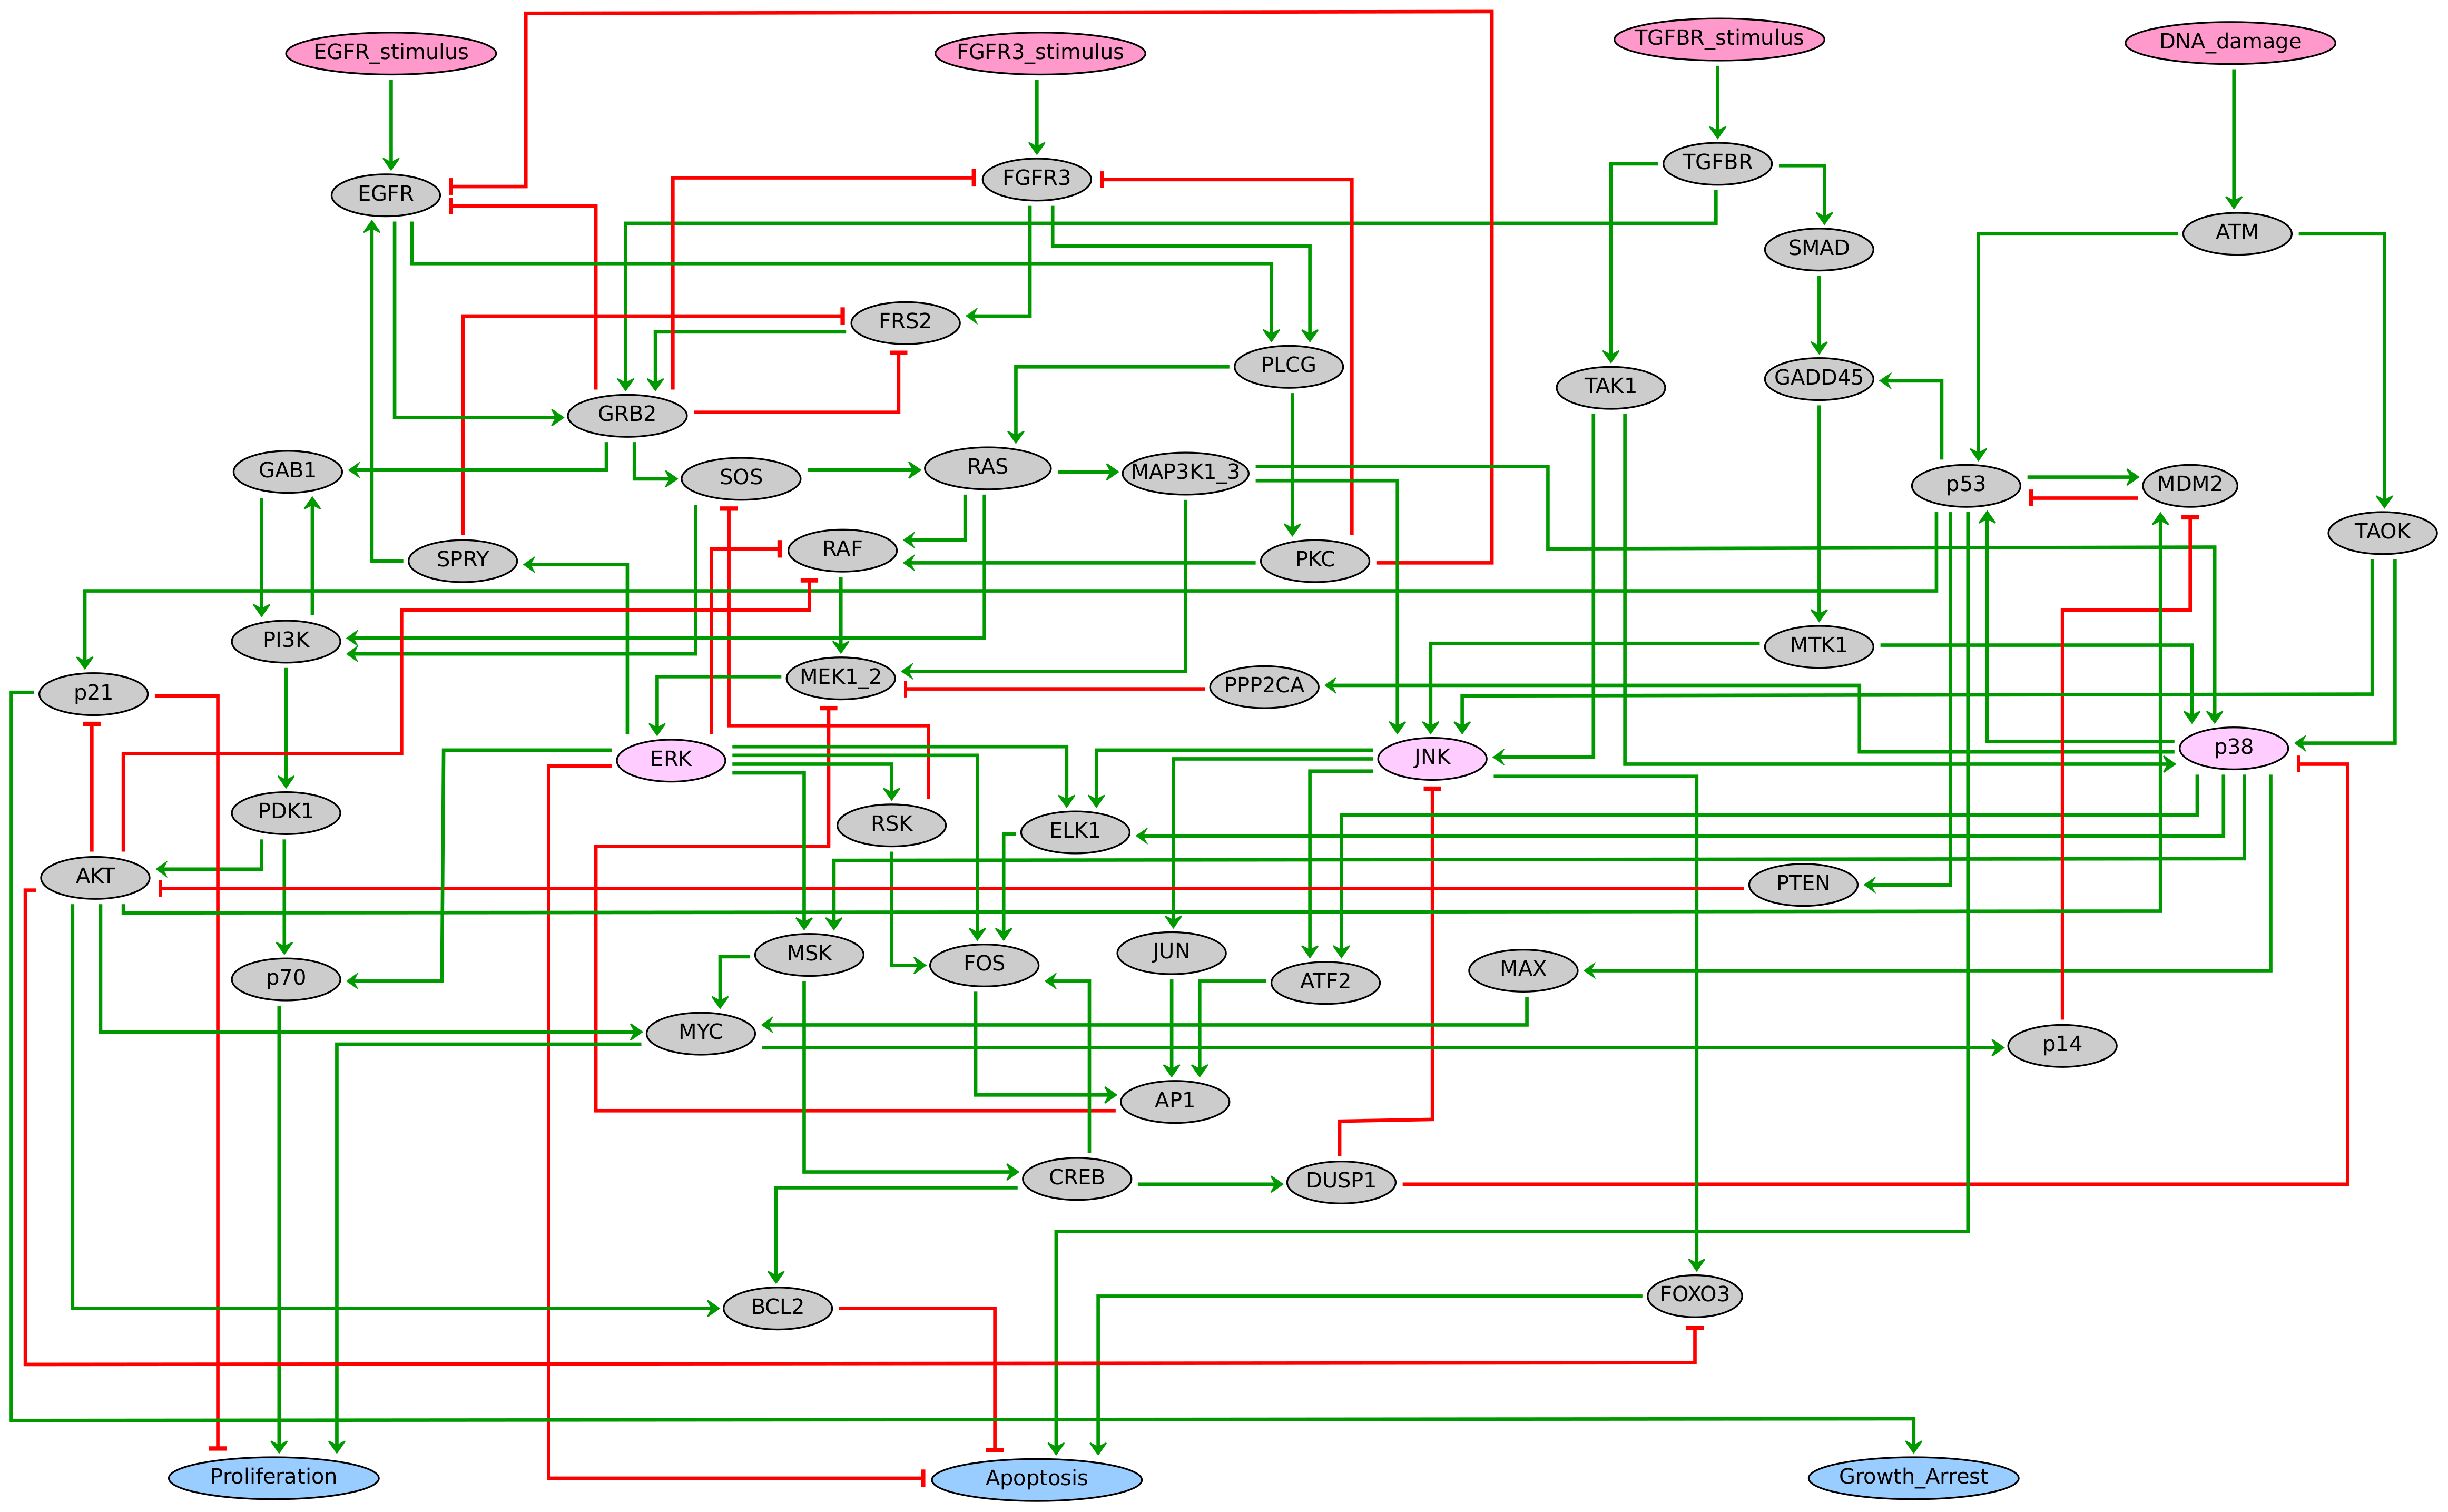
\includegraphics[width=\textwidth]{Figures/grieco_rg.png}
  \caption{\textbf{Regulatory network of the MAPK signalling pathway model.} The model consists of 53 variables and 104 regulatory interactions. The model is directly taken from~\cite{Grieco2013}}
  \label{fig:grieco_rn}
  \end{minipage}
}\end{figure}

% - Model introduction
% - Attractor (phenotype) classification
% - 0000 - control everything
%     - Former Grieco replication
% - ERK vs. (→) phenotypes ?

Another model we consider is the Grieco et al. version of MAPK model as presented in~\cite{Grieco2013}. This model represents a bladder cancer behavior using a combination of three pathways (FGFR3, EFGR, and TGFBR). The model has four inputs (a stimulus for each pathway and a DNA damage). We consider these inputs set to a constant false with an exception to FGFR3 which set to true (as in the previous model).

The regulatory network of the model can be found in \autoref{fig:grieco_rn}. The exact function definitions can be found in \autoref{appendix:digi_attach}.



% \begin{table}[]
% \checkoddpage
% \edef\side{\ifoddpage l\else r\fi}
% \makebox[\textwidth][\side]{% 
% \begin{minipage}[t]{\fullwidth}
% \scriptsize
% \caption{\textbf{Update functions of the isolated FGFR3 pathway modexl.} The table shows the update functions of the variables in the model as in~\cite{Grieco2013}. The variables are ordered alphabetically. The last four variables are inputs of the model.}
% \begin{tabular}{lp{15cm}}
% \hline
% \textbf{Variable} & \textbf{Function} \\
% \hline
% \var{AKT} & \var{PDK1} $\land$ \var{PTEN} \\
% \var{AP1} & \var{JUN} $\land$ (\var{ATF2} $\lor$ \var{FOS}) \\
% \var{ATF2} & \var{JNK} $\lor$ \var{p38} \\
% \var{ATM} & \var{DNA\_damage} \\
% \var{Apoptosis} & (\var{FOXO3} $\land$ \var{p53}) $\land$ $\neg$(\var{BCL2} $\lor$ \var{ERK}) \\
% \var{BCL2} & \var{CREB} $\land$ \var{AKT} \\
% \var{CREB} & \var{MSK} \\
% \var{DUSP1} & \var{CREB} \\
% \var{EGFR} & (\var{EGFR\_stimulus} $\land$ $\neg$(\var{PKC} $\lor$ \var{GRB2})) $\lor$ (\var{SPRY} $\land$ $\neg$(\var{PKC} $\lor$ \var{GRB2})) \\
% \var{ELK1} & (\var{JNK} $\lor$ \var{ERK}) $\lor$ \var{p38} \\
% \var{ERK} & \var{MEK1\_2} \\
% \var{FGFR3} & \var{FGFR3\_stimulus} $\land$ $\neg$(\var{PKC} $\lor$ \var{GRB2}) \\
% \var{FOS} & \var{ERK} $\land$ \var{RSK} $\land$ (\var{CREB} $\lor$ \var{ELK1}) \\
% \var{FOXO3} & \var{JNK} $\land$ $\neg$\var{AKT} \\
% \var{FRS2} & \var{FGFR3} $\land$ $\neg$(\var{GRB2} $\lor$ \var{SPRY}) \\
% \var{GAB1} & \var{PI3K} $\lor$ \var{GRB2} \\
% \var{GADD45} & \var{p53} $\lor$ \var{SMAD} \\
% \var{GRB2} & \var{EGFR} $\lor$ \var{TGFBR} $\lor$ \var{FRS2} \\
% \var{Growth\_Arrest} & \var{p21} \\
% \var{JNK} & (\var{TAOK} $\land$ \var{MAP3K1\_3}) $\lor$ (\var{TAK1} $\land$ $\neg$\var{DUSP1}) $\lor$ (\var{MAP3K1\_3} $\land$ \var{MTK1}) $\lor$ (\var{TAK1} $\land$ \var{MAP3K1\_3}) $\lor$ (\var{MAP3K1\_3} $\land$ $\neg$\var{DUSP1}) $\lor$ (\var{TAK1} $\land$ \var{v\_MTK1}) $\lor$ (\var{TAK1} $\land$ \var{TAOK}) $\lor$ (\var{TAOK} $\land$ \var{MTK1}) $\lor$ (\var{MTK1} $\land$ $\neg$\var{DUSP1}) $\lor$ (\var{TAOK} $\land$ $\neg$\var{DUSP1}) \\
% \var{JUN} & \var{JNK} \\
% \var{MAP3K1\_3} & \var{RAS} \\
% \var{MAX} & \var{p38} \\
% \var{MDM2} & (\var{AKT} $\land$ $\neg$\var{p14}) $\lor$ (\var{p53} $\land$ $\neg$\var{p14}) \\
% \var{MEK1\_2} & (\var{RAF} $\land$ $\neg$(\var{PPP2CA} $\lor$ \var{AP1})) $\lor$ (\var{MAP3K1\_3} $\land$ $\neg$(\var{PPP2CA} $\lor$ \var{AP1})) \\
% \var{MSK} & \var{p38} $\lor$ \var{ERK} \\
% \var{MTK1} & \var{GADD45} \\
% \var{MYC} & (\var{MSK} $\land$ \var{AKT}) $\lor$ (\var{MSK} $\land$ \var{MAX}) \\
% \var{PDK1} & \var{PI3K} \\
% \var{PI3K} & \var{GAB1} $\lor$ (\var{RAS} $\land$ \var{SOS}) \\
% \var{PKC} & \var{PLCG} \\
% \var{PLCG} & \var{EGFR} $\lor$ \var{FGFR3} \\
% \var{PPP2CA} & \var{p38} \\
% \var{PTEN} & \var{p53} \\
% \var{Proliferation} & \var{p70} $\land$ \var{MYC} $\land$ $\neg$\var{p21} \\
% \var{RAF} & (\var{PKC} $\land$ $\neg$(\var{ERK} $\lor$ \var{AKT})) $\lor$ (\var{RAS} $\land$ $\neg$(\var{ERK} $\lor$ \var{AKT})) \\
% \var{RAS} & \var{SOS} $\lor$ \var{PLCG} \\
% \var{RSK} & \var{ERK} \\
% \var{SMAD} & \var{TGFBR} \\
% \var{SOS} & \var{GRB2} $\land$ $\neg$\var{RSK} \\
% \var{SPRY} & \var{ERK} \\
% \var{TAK1} & \var{TGFBR} \\
% \var{TAOK} & \var{ATM} \\
% \var{TGFBR} & \var{TGFBR\_stimulus} \\
% \var{p14} & \var{MYC} \\
% \var{p21} & \var{p53} $\land$ $\neg$\var{AKT} \\
% \var{p38} & (\var{MAP3K1\_3} $\land$ \var{MTK1}) $\lor$ (\var{TAK1} $\land$ $\neg$\var{DUSP1}) $\lor$ (\var{TAOK} $\land$ \var{MAP3K1\_3}) $\lor$ (\var{MAP3K1\_3} $\land$ $\neg$\var{DUSP1}) $\lor$ (\var{TAK1} $\land$ \var{MAP3K1\_3}) $\lor$ (\var{TAOK} $\land$ $\neg$\var{DUSP1}) $\lor$ (\var{TAK1} $\land$ \var{MTK1}) $\lor$ (\var{TAK1} $\land$ \var{TAOK}) $\lor$ (\var{MTK1} $\land$ $\neg$\var{DUSP1}) $\lor$ (\var{TAOK} $\land$ \var{MTK1}) \\
% \var{p53} & (\var{p38} $\land$ $\neg$\var{MDM2}) $\lor$ (\var{ATM} $\land$ $\neg$\var{MDM2}) $\lor$ (\var{ATM} $\land$ \var{p38}) \\
% \var{p70} & \var{PDK1} $\land$ \var{ERK} \\
% \var{DNA\_damage} & \var{FALSE} \\
% \var{EGFR\_stimulus} & \var{FALSE} \\
% \var{FGFR3\_stimulus} & \var{TRUE} \\
% \var{TGFBR\_stimulus} & \var{FALSE} \\
% \hline
% \end{tabular}
% \label{tab:grieco_funs}
% \end{minipage}
% }
% \end{table}



Moreover, the MAPK model contains three outputs variables (apoptosis, growth arrest, proliferation). These outputs are then used to represent the four cardinal phenotypes of the model. These phenotypes and their exact configuration is depicted in \autoref{tab:grieco_phenotypes}.


\begin{table}[ht!]
  \checkoddpage
  \edef\side{\ifoddpage l\else r\fi}
  \makebox[\textwidth][\side]{% 
	\begin{minipage}[t]{\fullwidth}
  \small
  \caption{\textbf{MAPK phenotypes.} The cardinal phenotypes of the Grieco MAPK model which will be used throughout the experiments. The first two columns represent the full name and abbreviation of the phenotype. The last three columns represent the model output values which are representing a given phenotype.} 
  \centering
  \begin{tabular}{lc|ccc}
  \hline 
  \textbf{Phenotype} & \textbf{Abbreviation} & \textbf{Apoptosis} & \textbf{Growth arrest} & \textbf{Proliferation} \\
  \hline
  Apoptosis     & A & 1         & *             & 0             \\
  Growth arrest & GA & 0         & 1             & 0             \\
  Proliferation & P & 0         & 0             & 1             \\
  No decision   & ND & 0         & 0             & 0          \\
  \hline  \addlinespace
  \end{tabular}
  \label{tab:grieco_phenotypes}
  \end{minipage}
  }
\end{table}

\begin{table}[!htbp]
  \checkoddpage
  \edef\side{\ifoddpage l\else r\fi}
  \makebox[\textwidth][\side]{% 
	\begin{minipage}[t]{\fullwidth}
  \caption{\textbf{MAPK perturbations.} A list of perturbations of size up to 1 which drive the MAPK model to a phenotype given in the first column. An $\emptyset$ symbol stands for no perturbation while perturbations contained in the square brackets are needed to be combined in order to achieve the perturbation goal. The last column contains a count of unique smallest perturbations achieving the given phenotype.}
  \centering
  \begin{tabular}{lll}
  \textbf{Phenotype} & \textbf{Perturbations} & \textbf{\#}\\ \midrule
  Apoptosis & \begin{tabular}[c]{@{}l@{}}\blue{\var{ATM}=1; \var{CREB}=0; \var{DNA\_damage}=1; \var{DUSP1}=0; \var{FRS2}=1;} \blue{\var{GRB2}=1; \var{TAK1}=1;} \\ \blue{\var{TAOK}=1; \var{TGFBR}=1; \var{TGFBR\_st.}=1}\end{tabular} & 10 \\  [2ex]
  Growth arrest & \begin{tabular}[c]{@{}l@{}} [\var{AKT}=\var{p21}=1]; \blue{[\var{ATM}=\var{BCL2}=1]}; \blue{[\var{ATM}=\var{ERK}=1]}; \blue{$[$\var{ATM}=1,\var{FOXO3}=0]}; ... \end{tabular} & 85 \\ 
  No decision & \begin{tabular}[c]{@{}l@{}}\var{FGFR3}=0; \var{FGFR3\_st.}=0; \var{MAP3K1\_3}=0; \var{MSK}=0; \var{MYC}=0; \var{PKC}=1; \var{RAS}=0\end{tabular} & 7 \\ 
  Proliferation & \blue{\var{ERK}=1}; \var{MEK1\_2}=1; \var{RAF}=1 & 3\\ \midrule
  \begin{tabular}[c]{@{}l@{}}\oscil A-GA \end{tabular} & \var{p21}=1, \var{p38}=1, \var{p53}=1 & 3 \\ [1ex]
  \oscil A-ND & \begin{tabular}[c]{@{}l@{}} [\var{AP1}=1,\var{p21}=0]; [\var{ERK}=\var{p21}=0]; [\var{GRB2}=\var{p21}=0]; $[$\var{JNK}=1,\var{p21}=1]; ...\end{tabular} & 10 \\
  \oscil A-P & N/A & 0 \\ [1ex]
  \begin{tabular}[c]{@{}l@{}}\oscil GA-ND \end{tabular} & \begin{tabular}[c]{@{}l@{}} \blue{[\var{AP1}=\var{BCL2}=1]; [\var{AP1}=1,\var{FOXO3}=0]}; [\var{AP1}=1=\var{JNK}=0]; \blue{$[$\var{BCL2}=1,\var{ERK}=0]}; ... \end{tabular} & 26 \\
  \begin{tabular}[c]{@{}l@{}}\oscil GA-P \end{tabular} & N/A & 0 \\ [2ex]
  \begin{tabular}[c]{@{}l@{}}\oscil ND-P \end{tabular} & \begin{tabular}[c]{@{}l@{}} \var{AKT}=1; \var{CREB}=1; \var{DUSP1}=1; \var{MDM2}=1; \var{MSK}=1; \var{PTEN}=0; \var{p14}=0; \var{p21}=0; \\ \var{p38}=0; \blue{\var{p53}=0} \end{tabular} & 10 \\ \midrule
  \begin{tabular}[c]{@{}l@{}}\oscil A-GA-ND \end{tabular} & \begin{tabular}[c]{@{}l@{}} \var{AP1}=1; \var{ERK}=0; \var{GRB2}=0; \var{JNK}=1; \var{MEK1\_2}=0; \var{PDK1}=0; \var{PI3K}=0; \var{PPP2CA}=1;\\ \var{p70}=0 \end{tabular} & 9 \\ [2ex]
  \begin{tabular}[c]{@{}l@{}}\oscil A-GA-P \end{tabular} & N/A & 0 \\ [1ex]
  \begin{tabular}[c]{@{}l@{}}\oscil A-ND-P \end{tabular} & \begin{tabular}[c]{@{}l@{}} \var{p21}=0 \end{tabular} & 1 \\ [1ex]
  \begin{tabular}[c]{@{}l@{}}\oscil GA-ND-P \end{tabular} & \blue{\var{BCL2}=1}; \blue{\var{FOXO3}=0}; \var{JNK}=0 & 3 \\ \midrule
  \begin{tabular}[c]{@{}l@{}}\oscil $\forall$ \end{tabular} & $\emptyset$ & 1  \\ 
  \midrule
  \end{tabular}
      \label{tab:grieco_phenotypes_perturbations}
  \end{minipage}
  }
\end{table}

In the study~\cite{Grieco2013}, the full model version with 53 variables was presented. However, the simulations of knockout and over-expression experiments were performed on a reduced variant of the model (having only 17 variables) to observe how they impact the model phenotypes. Our novel approach allows us to consider the full model and all possible perturbations of the model at once, which helps us to obtain more comprehensive results. \autoref{tab:grieco_phenotypes_perturbations} shows the exhaustive enumeration of one-size perturbations which lead to any phenotype (as in \autoref{tab:grieco_phenotypes}), including all observed combinations of phenotype oscillations.


Stabilization in all phenotypes apart from growth arrest is possible with perturbations of size one. The unperturbed model behavior is an oscillation through all phenotypes. Moreover, disabling the only input set to true, \var{FGFR3\_stimulus}, causes the model to stabilize in the no-decision phenotype.

The results also highlight the influence of ERK, which represented the phenotype in the previous model. Since perturbing ERK leads to proliferation, ERK appears to be a strong driver of the proliferation phenotype. However, several previously observed drivers stabilizing ERK (from \autoref{sec:mapk_case_study_isolated}) are not present among the perturbations of the full model. This may be because the full model contains more variables, making their influence on ERK more complex.

% Last but not least, we can observe that the model as proposed in~\cite{Grieco2013} exhibits oscillations in numerous combinations of phenotypes under relatively small perturbations. Specifically, there are decisions containing oscillation between apoptosis and other phenotype. Such a behavior is difficult to interpret since a real-world system would be expected to continue in proliferation after committing to conduct the apoptosis. 

\subsection{Extended FGFR3 pathway MAPK}

To demonstrate our method on a larger-scale model, we extend the fully specified model~\cite{Grieco2013} that puts FGFR3-MAPK signalling into a broader context of protein interactions having the crucial impact on cell growth. The model has originally targeted bladder tissue cells. Our extension employs the PSBN framework allowing us to establish a partially specified model that incorporates mechanisms which are not yet understood well. In particular, based on Reactome~\cite{Milacic2023} and state-of-the-art knowledge~\cite{Fafilek2018,Fafilek2022} we compile an extended model bringing the updated FGFR3 activation mechanism to the Grieco model. 


\begin{table}[htbp!]
\checkoddpage
\edef\side{\ifoddpage l\else r\fi}
\makebox[\textwidth][\side]{% 
\begin{minipage}[t]{\fullwidth}
\caption{\textbf{Changes done to model MAPK model.} The table shows the changes done to the original model~\cite{Grieco2013} in order to obtain the extended model. The first column shows the variable and a type of the change. The second column shows the original list of regulations or functions. The third column shows the new list of regulations or functions with the changes highlighted in \textcolor{blue}{blue} font. The regulations marked with + are positives, - are negatives and ? denotes that regulation might not be present in an interpretation. Double ?? denotes that the regulation might be present in an interpretation as both positive and negative. Functions are denoted with $f$ and $g$ are the functions which are not specified in the model, but their instance must adhere to the listed regulations.}
\begin{tabular}{lll}
\hline
 &  \textbf{Original} & \textbf{New} \\
\hline
\var{FGFR3} reg. & \var{FGFR3\_stim}+, \var{GRB2}-, \var{PKC}- & \var{FGFR3\_stim}+, \var{GRB2}-\textcolor{blue}{?}, \var{PKC}-\textcolor{blue}{?} \\
 \var{FGFR3} def. & \var{FGFR3\_stim} $\land$ $\neg$(\var{GRB2} $\lor$ \var{PKC}) & \var{FGFR3\_stim} $\land$ \textcolor{blue}{$f$(\var{GRB2},\var{PKC})} \\
\var{FRS2} reg. & \var{FGFR3}+, \var{GRB2}-, \var{SPRY}- & \textcolor{blue}{\var{ERK}-?}, \var{FGFR3}+, \var{GRB2}-\textcolor{blue}{?}, \textcolor{blue}{\var{SHIP2}??}, \var{SPRY}-\textcolor{blue}{?} \\
\var{FRS2} def. & \var{FGFR3} $\land$ $\neg$(
\var{GRB2} $\lor$ \var{SPRY}) & \textcolor{blue}{$g$(\var{FGFR3},\var{ERK},\var{GRB2},\var{SHIP2},\var{SPRY})} \\
\hline
\end{tabular}
\label{tab:grieco_extension}
\end{minipage}
}
\end{table}

\begin{table}[htbp!]
\checkoddpage
\edef\side{\ifoddpage l\else r\fi}
\makebox[\textwidth][\side]{% 
\begin{minipage}[t]{\fullwidth}
\centering
\caption{\textbf{Extended MAPK model performance.} The table shows the performance of the extended MAPK model. The first column shows the phenotype, the second column shows the relation to the perturbation (standard, avoid, oscillation), and the third column shows the time of the computation. The computations were performed on a computer with AMD Ryzen Threadripper 2990WX 32-Core Processor and 64GB of memory.}
\begin{tabular}{llr}
\phenotype & \textbf{relation} & \multicolumn{1}{l}{\textbf{time}} \\
\hline
GA & standard & 00:02:45 \\
P & standard & 00:24:59 \\
A & standard & 00:35:59 \\
A & avoid & 00:39:26 \\
ND & avoid & 00:40:00 \\
GA & avoid & 00:41:56 \\
ND & standard & 01:13:09 \\
GA & oscillation & 01:17:13 \\
A & oscillation & 02:42:08 \\
P & avoid & 03:50:26 \\
ND & oscillation & 04:05:15 \\
P & oscillation & 13:09:52 \\
\hline
\end{tabular}
\label{tab:fgfr3extended_perf}
\end{minipage}
}
\end{table}




This is done by embedding the isolated FGFR3-MAPK pathway studied in previous section. At the level of regulations, the embedding brings in: 

\begin{enumerate}
  \item Addition of SHIP2 affecting the FRS2 adapter phoshorylation capabilities as discussed within the isolated model
  \item Addition of the positive feedback from ERK to FRS2 (experimentally studied mostly in the context of chondrocytes)
  \item Addition of the positive feedback from ERK to GRB2 (experimentally studied mostly in the context of chondrocytes)
\end{enumerate}

At the level of logical rules, the update functions of \var{FGFR3} and \var{FRS2} are made unspecified with the only constraint that \var{FGFR3\_stimulus} is left as a necessary precursor of \var{FGFR3} activation. The chosen level of abstraction reflects the fact that biochemical mechanisms specifying how the respective regulations affecting \var{FGFR3} and \var{FRS2} are combined are not currently known. Same as before, we consider the inputs to be fixed to 0, with an exception to FGFR3 stimulus. The resulting model contains 54 variables and four cardinal phenotypes as described in~\cite{Grieco2013} -- apoptosis (A), growth arrest (GA), no decision (ND), and proliferation (P). The exact overview of the model changes is available in the \autoref{tab:grieco_extension}.


\begin{figure}[htbp!]
  \centering
  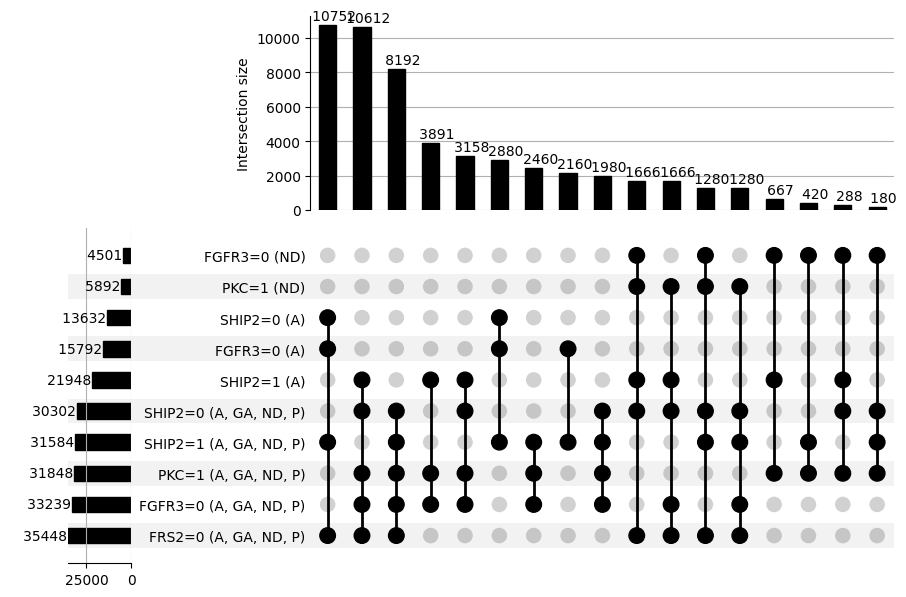
\includegraphics[width=\textwidth]{Figures/upset_extended.png}
  \caption{\textbf{Upset plot for the FGFR3 extended model.} The plot clearly shows, that each perturbation achieves a unique interpretation partitioning. Moreover, it is not possible to achieve two different phenotypes at once using the same perturbation. The perturbations are not unique, since we consider all phenotypes and perturbations at once.}
  \label{fig:extended_upset}
\end{figure}


The goal of the analysis is to apply control-guided refinement to identify perturbations that can reduce the set of possible interpretations of the extended PSBN. We consider the hypotheses on the FGFR3 signalling mechanisms stated in previous section and the pior knowledge based on~\cite{Grieco2013,Vaque2014,Stanislaus2012}.



First, we compute control for all phenotypes including oscillations among them. We restrict the results to perturbations of size up to 1. The performance results are shown in \autoref{tab:fgfr3extended_perf}. We can see, that our method was able to compute perturbations for all cardinal phenotypes in a reasonable time.

\sethlcolor{green!30}
\begin{table}[btph!]
  \caption{\textbf{Phenotype control of extended MAPK model.} The first column shows the (stable) phenotype or multiple oscillating phenotypes manifested by the model under perturbations listed in the second column. Perturbations in \textcolor{blue}{blue} font are working in the original~\cite{Grieco2013} model. Perturbations highlighted in \hl{green} are the reference perturbations we used for the model refinement. The third column displays the long-term ERK activity, and the last column shows the robustness of respective perturbations. The symbol '*' denotes that we observe amiguous ERK behavior under the given perturbations.}
  \centering
  \small
  \begin{tabular}{rlccc}
  \textbf{\phenotype} & \textbf{Perturbations} & ERK & $\robustness$ for $\allInterpretations$ & $\robustness$ for $\interpretationSet$ \\ \midrule
  A & \begin{tabular}[c]{@{}l@{}}\textcolor{blue}{\var{ATM}=1,\var{CREB}=0,\var{DNA\_dmg}=1,\var{DUSP1}=0},\\ \textcolor{blue}{\var{TAK1}=1,\var{TAOK}=1,\var{TGFBR}=1,\var{TGFBR\_st.}=1}\end{tabular} & 0 & 1 & 1\\
  & \varhl{PLCG}\hl{=0} & 0 & 0.80 & 1\\ 
  & \textcolor{blue}{\var{FRS2}=1,\var{GRB2}=1} & 0 & 0.64 & 1\\
  & \begin{tabular}[c]{@{}l@{}}\var{AP1}=1,\var{ERK}=0,\var{GADD45}=1,\var{JNK}=1,\var{JUN}=1,\\\var{MEK1\_2}=0,\var{MTK1}=1,\var{PPP2CA}=1,\var{SMAD}=1,\\ \var{p38}=1,\var{p53}=1,\var{SHIP2}=1,\var{SHIP2}=0,\var{PKC}=1,\\\O,\var{SPRY},\var{RSK}=0,\var{PKC}=0,\var{SPRY}=1 \end{tabular} & 0 & $<$0.6 & $<$0.5\\
  \midrule
  GA & \var{BCL2}=1,\var{FOXO3}=0,\var{JNK}=0 & 0 & 0.61 & 0 \\ 
  & \var{ERK}=1,\var{MEK1\_2}=0,\var{p21}=1 & 1 & $<$0.3 & 0 \\ 
  \midrule
  ND & \begin{tabular}[c]{@{}l@{}}\var{AKT}=1,\var{PTEN}=0;\var{p38}=0\end{tabular} & 0 & 0.61 & 0 \\ 
  & \begin{tabular}[c]{@{}l@{}}\textcolor{blue}{\var{MAP3K1\_3}=0,\var{MSK}=0,\var{MYC}=0,\var{RAS}=0} \end{tabular} & * & 0.50 & 1 \\ 
  & \begin{tabular}[c]{@{}l@{}}\var{AKT}=0,\textcolor{blue}{\var{FGFR3}=0},\var{GAB1}=0,\var{RSK}=1,\var{SOS}=0, \\ \textcolor{blue}{\var{FGFR3\_stimulus}=0},\var{p53}=0,\var{p70}=0, \\ \var{PDK1}=0,\var{PI3K}=0,\textcolor{blue}{\var{PKC}=1},\var{PLCG}=0,\var{PTEN}=1\end{tabular} & * & $<$0.3 & $<$0.2 \\ 
  \midrule
  P & \textcolor{blue}{\varhl{ERK}\hl{=1}, \var{MEK1\_2}=1} & 1 & 0.3 & 1 \\ 
  & \textcolor{blue}{\var{RAF}=1} & 1 & 0.19 & 1 \\ 
  & \begin{tabular}[c]{@{}l@{}}\var{GAB1}=1,\var{GADD45}=0,\var{MAX}=0,\var{MDM2}=1, \\ \var{MTK1}=0,\var{p14}=0,\var{p53}=0,\var{PDK1}=1,\var{PI3K}=1
  \end{tabular} & 1 & $<$0.1 & 0 \\
  \midrule

  A-GA & \textcolor{blue}{\var{p38}=1,\var{p53}=1} & 0 & 0.25 & 1 \\
  & \textcolor{blue}{\var{p21}=1} & * & 0.19 & 1 \\  

  ND-P & \begin{tabular}[c]{@{}l@{}} \textcolor{blue}{\var{p53}=0} \end{tabular} & \oscil & 0.55 & 1 \\ 
  & \begin{tabular}[c]{@{}l@{}} \textcolor{blue}{\var{MDM2}=1,\var{p14}=0},\textcolor{blue}{\var{AKT}=1,\var{CREB}=1,\var{DUSP1}=1,} \\ \textcolor{blue}{\var{MSK}=1,\var{PTEN}=0,\var{p38}=0} \end{tabular} & \oscil & $<$0.3 & 1 \\ 

  A-GA-ND & \begin{tabular}[c]{@{}l@{}} \textcolor{blue}{\var{AP1}=1,\var{ERK}=0,\var{JNK}=1,\var{MEK1\_2}=0,}\textcolor{blue}{\var{PPP2CA}=1}\end{tabular} & 0 & 0.25 & 1 \\ 
  & \begin{tabular}[c]{@{}l@{}}\textcolor{blue}{\var{GRB2}=0}\end{tabular} & \oscil & 0.2 & 0.6 \\   
  & \begin{tabular}[c]{@{}l@{}}\textcolor{blue}{\var{PDK1}=0, \var{PI3K}=0, \var{p70}=0}\end{tabular} & \oscil & $<$0.2 & 1 \\   


  A-ND-P & \begin{tabular}[c]{@{}l@{}} \textcolor{blue}{\var{p21}=0} \end{tabular} & \oscil & 0.19 & 1 \\  

  GA-ND-P & \textcolor{blue}{\var{BCL2}=1; \var{FOXO3}=0; \var{JNK}=0} & \oscil & 0.19 & 1 \\ \midrule
  \oscil $\forall$
  & \textcolor{blue}{\hl{\O}} & \oscil & 0.28 & 1 \\  
  \midrule
  \end{tabular}
  \label{tab:fgfr3extended}
\end{table}

\begin{table}[htb!]
  \caption{\textbf{Behavior of interpretations under perturbations of extended MAPK model.} The first column denotes the size of the interpretation set, while the next five columns denote the behavior of the interpretations under the selected perturbations. The $\mid$ separates possible bi-stability outcome while $\oscil$ denotes oscillation between all model phenotypes.}
\centering
  \begin{tabular}{r|ccccc}
  $\mid \interpretationSet \mid$ & \var{FGFR3}=0 & \var{FRS2}=0 & \var{PKC}=1 & \var{SHIP2}=0 & \var{SHIP2}=1 \\  \hline
  10752 & A        & $\oscil$         & A        & A             & $\oscil$         \\
  10612 & $\oscil$ & $\oscil$         & $\oscil$ & $\oscil$      & A                \\
  8192  & $\oscil$ & $\oscil$         & $\oscil$ & $\oscil$      & $\oscil$         \\
  3848  & $\oscil$ & A$\mid$ND$\mid$P & $\oscil$ & ND$\mid$P     & A                \\
  3158  & $\oscil$ & A$\mid$ND$\mid$P & $\oscil$ & $\oscil$      & A                \\
  2880  & A        & A$\mid$ND$\mid$P & A        & A             & $\oscil$         \\
  2430  & $\oscil$ & A$\mid$ND$\mid$P & $\oscil$ & ND$\mid$P     & $\oscil$         \\
  2160  & A        & A$\mid$ND$\mid$P & A        & A$\mid$ND$\mid$P & $\oscil$     \\
  1980  & $\oscil$ & A$\mid$ND$\mid$P & $\oscil$ & $\oscil$      & $\oscil$         \\
  1666  & ND       & $\oscil$         & ND       & $\oscil$      & A                \\
  1666  & $\oscil$ & $\oscil$         & ND       & $\oscil$      & A                \\
  1280  & ND       & $\oscil$         & ND       & $\oscil$      & $\oscil$         \\
  1280  & $\oscil$ & $\oscil$         & ND       & $\oscil$      & $\oscil$         \\
  624   & ND       & A$\mid$ND$\mid$P & $\oscil$ & ND$\mid$P     & A                \\
  390   & ND       & A$\mid$ND$\mid$P & $\oscil$ & ND$\mid$P     & $\oscil$         \\
  288   & ND       & A$\mid$ND$\mid$P & $\oscil$ & $\oscil$      & A                \\
  180   & ND       & A$\mid$ND$\mid$P & $\oscil$ & $\oscil$      & $\oscil$         \\
  43    & ND       & A$\mid$ND$\mid$P & $\oscil$ & A$\mid$ND$\mid$P & A            \\
  43    & $\oscil$ & A$\mid$ND$\mid$P & $\oscil$ & A$\mid$ND$\mid$P & A            \\
  30    & $\oscil$ & A$\mid$ND$\mid$P & $\oscil$ & A$\mid$ND$\mid$P & $\oscil$     \\
  30    & ND       & A$\mid$ND$\mid$P & $\oscil$ & A$\mid$ND$\mid$P & $\oscil$     \\
  \end{tabular}
  \label{tab:fgfr3extended_phenotypes}
  \end{table}

The results are shown in \autoref{tab:fgfr3extended}. We can see, that perturbations can achieve all the four cardinal phenotypes as well as achievable oscillations among them. We can also observe the correlation between the ERK activity and the proliferation phenotype -- in particular, the ERK stabilization is required for the proliferation phenotype, while apoptosis phenotype drives ERK avoidance.

The results highlighted in blue correspond with the perturbations computed on the original model~\cite{Grieco2013} (see \autoref{tab:grieco_phenotypes_perturbations}). Moreover, the results include several perturbations that have not been observed before. Notably, there is the perturbation \var{PLCG}=0 which leads to apoptosis stabilization. This perturbation is not present in the original model, however, it has been observed in~\cite{Vaque2014,Stanislaus2012} that PLCG is a driver for cell proliferation while its inhibition can lead to apoptosis. This is a strong evidence that this perturbation is indeed valid, and we can use it for our model refinement.

Based on the discussion above, the perturbations \var{ERK}=1 (achieving proliferation) and \var{PLCG}=0 (leading to apoptosis) are strongly affecting the long-term behavior of the model. To that end, we use this knowledge to complete the first iteration of the control-guided refinement procedure.



Analogously to the isolated model case study, we compute the new control results shown in the last column of \autoref{tab:fgfr3extended}. 


Next, we select perturbations achieving partitioning to distinct behavior patterns. Due to a big number of viable perturbations with non-100\% robustness, we first cross-compared all combinations of perturbations and phenotypes they achieve, to obtain a set of perturbation equivalence classes. Such equivalence classes were 10 having 1-3 members. Then, we selected one perturbation from each equivalence class. To verify, that they are indeed unique, we show their intersections in \autoref{fig:extended_upset}. Since we consider all phenotypes and perturbations at once, the perturbations are not unique. With upset diagram, we confirmed that all perturbations help with the interpretation classes partitioning unique and, that no perturbation achieves two different phenotypes at once what is expected for the correctness of our method. 


As a result we obtain only five distinct perturbations promising for the model refinement. The perturbations are shown in \autoref{tab:fgfr3extended_phenotypes}. The table displays the admissible perturbations that can be considered for \emph{in vitro} perturbation experiments design leading to potential exclusion of non-complying interpretations of the PSBN. The wet lab testing is necessary to complete the second iteration of the model refinement process, as illustrated in \autoref{fig:control_workflow}. 

\section{Summary}

In this chapter, we have demonstrated the applicability of our method on two case studies. The primary application of control was to make cell reprogramming perturbations. This type of application is commonly used for therapy design, where the goal is to find perturbations that can drive the system from a diseased state to a healthy one. We have shown the application on a myeloid differentiation model, where we have found perturbations that can drive the system between different types of cell differentiations.

Next, we have shown a framework for the model refinement using control. We have applied this framework on a MAPK model variants where we demonstrated how to use the control results to refine the model and reduce the set of possible interpretations either analytically or searching for perturbations that can be used for the wet lab experiments design.

\cleardoublepage

% Visually separate conclusions from other chapters in TOC

\chapter*{Conclusions}
\label{chapter:conclusion}
\addcontentsline{toc}{chapter}{\textsc{Conclusions}}
\addtocontents{toc}{\protect\bigskip}

Conclude here...

\cleardoublepage

%----------------------------------------------------------------------------------------
%	THESIS CONTENT - APPENDICES
%----------------------------------------------------------------------------------------

\appendix


\chapter{Notation}
\label{app:notation}

\begin{longtable}{@{}ll@{}}
    \multicolumn{2}{c}{\textbf{Boolean algebra related symbols}} \\
    $b$ & Boolean value (true or false) \\
    \bools & Set of Boolean values (true or false) \\
    \unspecified & Undefined Boolean value (might be true or false) \\ 
    $f$ & A function \\
    $\bools_{\unspecified}$ & Set of Boolean values including the undefined value \\
    $x[i \mapsto b]$ & A vector $x$ with the $i$-th element replaced by $b$ \\[2ex]
    \multicolumn{2}{c}{\textbf{Networks - common}} \\
    $n$ & Size of a network (number of its nodes -- variables) \\
    $\rnMath$ & Regulatory network \\
    $\vertices$ & Vertices of a network \\
    $\edges$ & Edges of a network \\
    \subspace & Subspace of a network \\
    \bnMath & Boolean network instance \\
    $\STG$ & Asynchronous state transition graph \\
    \run & A run (trajectory) of a (partially specified) Boolean network \\
    \essential(\var{var1, var2}) & Influence of \var{var1} on \var{var2} is observable in \STG \\
    \var{var} & A font for variable names \\
    \attractor & An attractor of a (partially specified) Boolean network \\
    $\allAttractors$ & Set of all attractors of a (partially specified) Boolean network \\
    \character & An observed character of a network \\
    \trait & A trait of a network \\
    \phenotype & A phenotype of a network \\ [2ex]
    \multicolumn{2}{c}{\textbf{Partially specified Boolean networks}} \\
    \pbnMath & Partially specified Boolean network \\
    $\funSymbol$ & A function symbol of a partially specified Boolean network \\
    $\allFunSymbols$ & Set of all function symbols of a partially specified Boolean network \\
    $\expr$ & An expression of a partially specified Boolean network \\
    $\interpretation$ & An interpretation of a partially specified Boolean network \\
    $\interpretationSet$ & A set of interpretations \\
    $\allInterpretations$ & Set of all interpretations of a partially specified Boolean network \\ [2ex]
    \multicolumn{2}{c}{\textbf{Control}} \\
    $\perturbation$ & A perturbation of a network \\
    $\allPerturbations$ & A set of all admissible perturbations \\
    $\robustness$ & Robustness of a perturbation towards considered set of interpretations \\
\end{longtable}

\chapter{Digital Attachments}

Lorem Ipsum..

%----------------------------------------------------------------------------------------
%	POST-CONTENT THESIS PAGES
%----------------------------------------------------------------------------------------

\cleardoublepage\include{FrontBackMatter/Bibliography} % Bibliography

%\cleardoublepage% Acknowledgements

\pdfbookmark[1]{Declaration}{Acknowledgements} % Bookmark name visible in a PDF viewer

\begingroup

\let\clearpage\relax
\let\cleardoublepage\relax
\let\cleardoublepage\relax

\chapter*{Declaration}
\addcontentsline{toc}{chapter}{\textsc{Declaration}}

Hereby I declare that this thesis is my original authorial work, which I have worked out on my own. All sources, references, and literature used or excerpted during the elaboration of this work are properly cited and listed in completed reference to the due source.
During the preparation of this thesis, I used the following AI tools
to improve the clarity and style of my writing:
\begin{itemize}
    \item Grammarly
    \item ChatGPT
    \item GitHub Copilot
\end{itemize}
Additionally, I used the following tool to assist with software development:
\begin{itemize}
    \item GitHub Copilot
\end{itemize}
I declare that I used these tools in accordance with the principles of
academic integrity. I checked the content and took full responsibility
for it.


\vspace*{1cm}

\hspace*{0pt}\hfill Eva Šmijáková


\endgroup

 % Declaration

%\cleardoublepage\include{FrontBackMatter/Colophon} % Colophon

%----------------------------------------------------------------------------------------

\end{document}
